\documentclass[12pt,twoside,openright,a5paper]{book}
\usepackage[margin=0.75in]{geometry}
\usepackage{layout}
\usepackage{pgffor}
\usepackage{tocloft}
\usepackage[table, dvipsnames]{xcolor}
\usepackage{fontspec}
\usepackage{fancybox}
\usepackage[skins]{tcolorbox}
\usepackage{fancyhdr}
\usepackage{setspace}
\usepackage[utf8]{inputenc}
\usepackage{emptypage}
\usepackage[vskip=0pt,rightmargin=0cm]{quoting}
\usepackage{sectsty}
\usepackage{polyglossia}
\usepackage{changepage}%
\usepackage{imakeidx}
\usepackage{setspace}
\usepackage{longtable,array}
\usepackage{tikz} % Package for drawing
\usepackage{tikzpagenodes}
\usepackage[toc,acronym]{glossaries}
\usepackage{fontawesome5}
\usepackage{marvosym}
\usepackage[totoc, font=footnotesize]{idxlayout}
\usepackage{eso-pic} % background image in titlepage
\usepackage{anyfontsize} % any font size



%\newcommand{\slcol}[1]{{\color{MidnightBlue}{#1}}}
%\newcommand{\cquote}[1]{\begin{quoting}{\color{darkgray}{#1}}\end{quoting}}
%\newcommand\Chapter[2]{
%  \chapter[#1]{#1\\\large#2}
%}
\newcommand\Chapter[2]{
  \chapter[#1 #2]{#1\\\Large{#2}}
  \vspace{-10mm}
  \newpgfornamentfamily{vectorian}
  \begin{center}
    
    \pgfornament[anchor=center,ydelta=0pt,width=5cm, color=black]{84}
  \end{center}
  %print different header for each chapter
  \fancyhead[RO]{\footnotesize \kanfont ಗೀತಾ ಮನನಂ} %Odd page Right
  \fancyhead[LO]{\footnotesize #1} % Odd page Left
  \fancyhead[LE]{\footnotesize \kanfont ಗೀತಾ ಮನನಂ} %Even page Left
  \fancyhead[RE]{\footnotesize #1} %Even page Right
}

\newcommand\NewHeader[1]{
  %print different header for each chapter
  \fancyhead[RO]{\footnotesize \kanfont ಗೀತಾ ಮನನಂ} %Odd page Right
  \fancyhead[LO]{\footnotesize #1} % Odd page Left
  \fancyhead[LE]{\footnotesize \kanfont ಗೀತಾ ಮನನಂ} %Even page Left
  \fancyhead[RE]{\footnotesize #1} %Even page Right
}
%
%\addto\captionskannada{\renewcommand{\contentsname}{\color{blue}{ವಿಷಯ ಸೂಚಿ}}}
%
% Font definitions
%
%\newfontfamily\mananamfont[Script=Kannada]{NudiUni08k}
%\newfontfamily\mananamtext[Script=Kannada]{AdishilaVedic}
%\newfontfamily\engfont[Script=Kannada]{Arial Unicode MS}
%
%
%\newcommand{\chapindexpage}{\thechapter-\arabic{page}}
%\renewcommand{\thepage}{\chapindexpage}
%\newcommand{\chapIndex}{\thechapter-\thepage}
%\newcommand\Index[1]{#1\index{#1, \thechapter}}
%\newcommand{\Index}[1]{#1\index{#1|chapIndex}}
\newcommand\chapEnd{
  \begin{center}
    \newpgfornamentfamily{vectorian}
    \pgfornament[anchor=center,ydelta=0pt,width=5cm, color=black]{85}  
  \end{center}
}
\newcommand{\chapEndSloka}[1]{
  \begin{center}
    {\color{black}\small
    ಇತಿ ಶ್ರೀಮದ್ಭಗವದ್ಗೀತಾ  ರೂಪೀ ಉಪನಿಷತ್, ಬ್ರಹ್ಮವಿದ್ಯಾ, ಯೋಗಶಾಸ್ತ್ರ\\ ವಿಷಯವಾಗಿ ಶ್ರೀಕೃಷ್ಣ ಹಾಗೂ ಅರ್ಜುನರ ಸಂವಾದದಲ್ಲಿ, \\‘#1’ ಎಂಬ ಅಧ್ಯಾಯ  ಸಂಪೂರ್ಣ}
  \end{center}
  \chapEnd
}
\newskip\linepagesep \linepagesep 5pt\relax
\renewcommand\footrulewidth{0.5pt}
\def\vfootline{%
    \begingroup
        \color{blue}\rule[-990pt]{20pt}{1000pt}
    \endgroup}


\newfontfamily\aksharfont[Script=Kannada]{Arial Unicode MS}
\setmainfont[Script=Kannada]{Arial Unicode MS}
\setmainlanguage{kannada}
\setotherlanguages{english}
\newfontfamily\kannadafont[Script=Kannada]{Arial Unicode MS}
\newfontfamily\kannadafontsf[Script=Kannada]{Arial Unicode MS}
\newfontfamily\kanfont[Script=Kannada]{Arial Unicode MS}

\fancyhf{}
  \fancyfoot[RO]{\vfootline\hskip\linepagesep\thepage}
  \fancyfoot[LE]{\thepage\hskip\linepagesep\vfootline}
  \fancyhead[RO]{\small\kanfont ದಿನಾಂಕ ..../..../.....}
  \fancyhead[LO]{\small\kanfont ಗೀತಾ ಮನನಂ}
  \fancyhead[LE]{\small\kanfont ಗೀತಾ ಮನನಂ}
  \fancyhead[RE]{\small\kanfont ದಿನಾಂಕ ..../..../.....}
  \renewcommand\headrulewidth{1pt}
  \fancypagestyle{plain}{%
    \fancyhf{}
    \fancyfoot[RO]{\vfootline\hskip\linepagesep\thepage}
    \fancyfoot[LE]{\thepage\hskip\linepagesep\vfootline}
    \renewcommand\headrulewidth{0pt}
  }
\quotingsetup{font={itshape,footnotesize}}
\title{\Huge \kanfont ಗೀತಾ ಮನನಂ\\Gita Mananam\\\small(ದೈನಂದಿನ ಸ್ಪೂರ್ತಿ ಹಾಗೂ ಆತ್ಮಾವಲೋಕನಕ್ಕಾಗಿ)}
\author{\large \kanfont ಸ್ವಾಮಿ ನಿರ್ಗುಣಾನಂದಗಿರಿ\\Swamy Nirgunanandagiri}

\renewcommand*\contentsname{\kanfont ವಿಷಯ ಸೂಚಿ}
\addto{\captionsenglish}{\renewcommand*{\contentsname}{\kanfont ವಿಷಯ ಸೂಚಿ}}

% Reduce space between TOC
\setlength\cftparskip{-2pt}
\setlength\cftbeforechapskip{2pt}
\setcounter{secnumdepth}{-1}
\chapterfont{\color{blue}}  % sets colour of chapters
\setlength\parindent{0pt} % no-indent for entire file
\date{} % clear date
\makeindex
\indexsetup{othercode=\small}


\newcommand\Linepage[1][0.40in]{% Change to suit
  \vbox to \dimexpr\textheight-\pagetotal-#1\relax {% Let TeX do the work...
    \leaders\hbox to \linewidth{\rule{0pt}{#1}\hrulefill}\vfil
  }%
}

\newtcolorbox{inspiration}[2][]{%
  floatplacement=b,float, 
  enhanced,colback=white,colframe=purple,coltitle=black,
  sharp corners,boxrule=1pt, width=\textwidth,
  fonttitle=\sffamily\scshape\color{teal},
  rightrule=3mm,
  fontupper=\itshape,
  fontlower=\tiny,
  attach boxed title to top left={yshift=-0.5\baselineskip-0.4pt,xshift=2mm},
  boxed title style={tile,size=minimal,left=0.5mm,right=0.5mm,
    colback=white,before upper=\strut},
  title=#2,#1
}
\newtcolorbox{mananam}[2][fontlower=\small]{%
  enhanced,colback=white,colframe=teal,coltitle=black,
  sharp corners,boxrule=1pt, width=\textwidth,
  fonttitle=\sffamily\scshape\color{purple},
  leftrule=3mm,
  fontupper=\itshape,
  fontlower=\tiny,
  attach boxed title to top left={yshift=-0.5\baselineskip-0.4pt,xshift=4mm},
  boxed title style={tile,size=minimal,left=0.5mm,right=0.5mm,
    colback=white,before upper=\strut},
  title=#2,#1
}

\newcommand\Index[1]{#1\index{#1}}

\newcommand\wave{%
  \begin{tikzpicture}[overlay,remember picture]
    \fill[red,line width=.5mm,draw=red] (current page.north west) circle (3mm);
    \def\max{20}
    \foreach \i in {4,...,\max} {
      \draw[red,line width=.5mm,draw opacity={(\max-\i)/(\max-4)}]
      (current page.north west) ++(\i mm,0)
      arc[start angle=0,end angle=-90,radius=\i mm];
    }
  \end{tikzpicture}%
}

\definecolor{pastelblue}{rgb}{0.68, 0.78, 0.81}

% commands
\definecolor{aurometalsaurus}{rgb}{0.43, 0.5, 0.5}

\begin{document}
\pagenumbering{roman}
\begin{titlepage}
	%\pagecolor{pastelblue}
	%\AddToShipoutPictureBG*{%
    %\AtPageLowerLeft{%
    %    \includegraphics[width=\paperwidth,height=\paperheight]{./images/krishna4.jpg}%
    %}%
%}
    \begin{center}
        \vspace*{0.5cm}
            
        {\Huge
        \textbf{\color{blue}\fontsize{50}{60}\selectfont ಗೀತಾ ಮನನಂ}}
        \textbf{\\ \small \color{black}ದೈನಂದಿನ ಸ್ಪೂರ್ತಿ ಹಾಗೂ ಆತ್ಮಾವಲೋಕನಕ್ಕಾಗಿ}    
        \vspace{3.0cm}\\
        \textbf{{\Large \color{blue}\mananamfont ಸ್ವಾಮಿ ನಿರ್ಗುಣಾನಂದ ಗಿರಿ}}\\    
        
		
            
        \vfill
            
        
            
        \vspace{0.1cm}
        {\color{black}    
		
		{{\large \color{blue}ಹೃಷೀಕೇಶ, ಉತ್ತರಾ ಖಂಡ}\\\normalsize ಭಾರತ}
        }
    \end{center}
\end{titlepage}
\nopagecolor% Use this to restore the color pages to white


\thispagestyle{empty}
Copyright \textcopyright\ Swamy Nirgunanandagiri\\
\\
All rights reserved\\
\\
Edition - First, 2024\\
\vfill
Without written permission of the author it is forbidden to reproduce or adapt in any form or by any means any part of this  publication.\\
\\
Rishikesh, India\\
\newpage
\thispagestyle{empty}
\tableofcontents

\begin{tikzpicture}[remember picture,overlay]
\node[anchor=east,inner sep=0pt] at (current page text area.east|-0cm,13.5cm) {\includegraphics[height=4cm]{./images/pic1.jpg}};
\end{tikzpicture}
\thispagestyle{empty}
\thispagestyle{empty}
\pagestyle{fancy}
\chapter{\kanfont ಮುನ್ನುಡಿ}

%\thispagestyle{empty}
\begin{onehalfspace} 
\chapter{\kanfont ಪ್ರಸ್ತಾವನೆ}
\textit{\indent ನಾವೆಲ್ಲರೂ ಜೀವನದ ಹೋರಾಟಗಳನ್ನು ಎದುರಿಸಬೇಕು. ಕುರುಕ್ಷೇತ್ರ ಯುದ್ಧದಲ್ಲಿ ಶ್ರೀ ಕೃಷ್ಣ ಪರಮಾತ್ಮ ತನ್ನ ವೇದನೆಯುಕ್ತ ಶಿಷ್ಯ ಅರ್ಜುನನಿಗೆ ಅಧ್ಯಾತ್ಮಿಕ ಹಾದಿಯಲ್ಲಿ ಆಚರಣೆಗೆ ತರುವಂತ ಬಹಳ ಪವಿತ್ರವಾದ ಬೋಧನೆಗಳನ್ನು ಕೊಟ್ಟಿದ್ದಾನೆ. ಈ ಶ್ರೇಷ್ಠವಾದ ಉಪನಿಷತ್ತುಗಳ ಸತ್ವಗಳನೊಳಗೊಂಡ  ಬೋಧನೆಗಳನ್ನು ಪವಿತ್ರವಾದ ಭಗವದ್ಗೀತೆಯನ್ನು ಸಂತ ವೇದವ್ಯಾಸರು ನಮ್ಮ ಕೈಗೆ ನೀಡಿದ್ದಾರೆ.\\
\\
 ಅರ್ಜುನನು ಇದ್ದ ಪರಿಸ್ಥಿತಿಗೂ ನಾವು ಇರುವ ಪರಿಸ್ಥಿತಿ ಮತ್ತು ಸಂಘರ್ಷಗಳಿಗೂ ವ್ಯತ್ಯಾಸಗಳಿರಬಹುದು. ಸಾರ್ವರ್ತಿಕ ಉಪದೇಶಗಳು ಸತ್ಯಾನ್ವೇಷಣೆ ಮಾಡಲು ಬಯಸುವ ಎಲ್ಲರಿಗೂ ಆತ್ಮೋನತಿ  ಮತ್ತು ಅಧ್ಯಾತ್ಮಿಕ ಪ್ರಗತಿ ಸಾಧಿಸಲು ಬೇಕಾಗುವ ಮಾದರಿಯಾಗಿದೆ.\\
\\
 ಭಗವದ್ಗೀತೆಯ ಉಪದೇಶಗಳು ಕೇವಲ ಆಧ್ಯಾತ್ಮಿಕ ಅನ್ವೇಷಣೆ ಮಾಡುವವರಿಗೆ ಸಮರ್ಪಿತವಾದದ್ದು ಮಾತ್ರವಲ್ಲದೆ ಜೀವನದಲ್ಲಿ ಬೇಕಾಗುವ ಅತ್ಯಮೂಲ್ಯವಾದ ಕೈಪಿಡಿಯಾಗಿದೆ. ಯಾರು ಕೆಲಸದ ಸಮತೋಲನ ಮತ್ತು ಕೌಟುಂಬಿಕ ಜವಾಬ್ದಾರಿಗಳನ್ನು ಮಾನಸಿಕ ನೆಮ್ಮದಿ ಮತ್ತು ಒತ್ತಡ ರಹಿತವಾಗಿ ಮಾಡಲು ಬಯಸುತ್ತಾರೋ ಅವರಿಗೆ ಈ ಬೋಧನೆಗಳು ತುಂಬಾ ಮಹತ್ವದ್ದಾಗಿ ಕಾಣುತ್ತದೆ.\\
\\
 ಅನೇಕ ಗುರುಗಳು ಮತ್ತು ವಿದ್ವಾಂಸರು ಆಗಲೇ ಮಾಡಿರುವಂತೆ ಈ ದಿನಚರಿ ಪುಸ್ತಕ ಮತ್ತು ನಿಯತಕಾಲಿಕವು, ಗೀತೆಯ ಬೋಧನೆಗಳನ್ನು ತಿಳಿಸುವ ಪ್ರಯತ್ನ ಅಥವಾ ವ್ಯಾಖ್ಯಾನ ಕೊಡುವುದಾಗಿಲ್ಲ. ಈ ಗೀತಾ ಮನನವು ಬೋಧನೆಗಳ ಚಿಂತನೆ ಮಾಡುವುದು ಮತ್ತು ಅದನ್ನು ನಮ್ಮ ಸ್ವಂತದ್ದನ್ನಾಗಿ ಮಾಡಿಕೊಳ್ಳುವುದಾಗಿದೆ. ದೇವ ನಾಗರಿಯಲ್ಲಿರುವ `ಮನನ` ಎಂಬ ಪದವು ಆಗಲೇ ಕೇಳಿದ್ದನ್ನು ಅಥವಾ ಓದಿದ್ದನ್ನು ಚಿಂತನೆ ಮಾಡುವ ಕಾರ್ಯವಿಧಾನವನ್ನು ಅನ್ವಯಿಸುವುದಾಗಿದೆ.\\
\\
 ಈ ದಿನಚರಿ ಪುಸ್ತಕವನ್ನು ನೀವು ನಿಮ್ಮ ಮನಸ್ಸಿನ ಇಂಗಿತವನ್ನು ಸ್ವಾತಂತ್ರ್ಯವಾಗಿ ವ್ಯಕ್ತಪಡಿಸಲು ದಾರಿ ಮಾಡಿಕೊಳ್ಳುವುದಕ್ಕೆ ಮತ್ತು ನಿಮ್ಮ ಜೀವನದಲ್ಲಿ ಅಳವಡಿಸಿಕೊಳ್ಳಲು ಉದ್ದೇಶದಿಂದ ರೂಪಿಸಲಾಗಿದೆ. ಗೀತೆಯಲ್ಲಿರುವ ಶ್ಲೋಕಗಳಲ್ಲಿನ ಪ್ರಶ್ನೆಗಳು ಈ ಬೋಧನೆಗಳ ಸನ್ನಿವೇಶಕ್ಕೆ ಸಂಬಂಧಿಸಿದಂತೆ, ನಿಮ್ಮ ವೈಯಕ್ತಿಕ ಅರ್ಥಗಳನ್ನು ಹುಡುಕಲು ಮತ್ತು ಅದರಿಂದ ಜೀವನದ ಸಂದರ್ಭದೊಳಗೆ ನಿಶ್ಚಲವಾದ ಸ್ಪಷ್ಟನೆ ಹುಡುಕಲು ರೂಪಿಸಲಾಗಿದೆ.ಶ್ರೀ ಕೃಷ್ಣ ಪರಮಾತ್ಮನು ಹೇಗೆ ಅರ್ಜುನನಿಗೆ ನ್ಯಾಯವಾದ ಯುದ್ಧವನ್ನು ಮಾಡಲು ಪ್ರೇರೇಪಿಸಿದಂತೆ ನಿಮ್ಮ ಜೀವನದ ಕರ್ತವ್ಯಗಳನ್ನು ಈ ಗೀತೆ ಎಂಬ ಕೆಲಸದಿಂದ,ಆ ಭಗವಂತ ನಿಮಗೂ ಪ್ರೇರೇಪಿಸಲಿ ಎಂದು ನಂಬುತ್ತೇನೆ. ನಿಮ್ಮ ಕರ್ತವ್ಯಗಳನ್ನು ಕುಶಲತೆಯಿಂದ ಯಶಸ್ವಿಯಾಗಿ ನಿರ್ವಹಿಸಲು ನಿಮ್ಮ ಅಂತರಂಗದ ಶಾಂತಿಯನ್ನು ಉಪಯೋಗಿಸದೆ ವೈಯಕ್ತಿಕ ಪ್ರಗತಿ ಮತ್ತು ದೈವತ್ವಕ್ಕೆ ನಂಬಿಕೆಯಿಂದ ಇರುವ ನಿರಂತರ ಉದ್ದೇಶದಿಂದ ಕೂಡಿರುವುದೇ ಈ ದಿವ್ಯವಾದ ಗೀತೆ.}

\end{onehalfspace}
\Chapter{\kanfont ೧ ಅರ್ಜುನ ವಿಶಾದ ಯೋಗ}{ಅಥ ಪ್ರಥಮೋऽಧ್ಯಾಯಃ}
\pagenumbering{arabic}
ಅಥ ಪ್ರಥಮೋऽಧ್ಯಾಯಃ ।\\
ಮೊಟ್ಟ ಮೊದಲನೆಯ ಶ್ಲೋಕವೇ ನಮಗೆ ಚಿಂತನೆ, ಮನನ ಪ್ರಾರಂಭಿಸಲು ಬೇಕಾಗುವ ಸೂಕ್ಷ್ಮವಾದ ಸಂದೇಶವನ್ನು ಕೊಡುತ್ತದೆ.\\
\slcol{ಧೃತರಾಷ್ಟ್ರ ಉವಾಚ ।\\
ಧರ್ಮಕ್ಷೇತ್ರೇ ಕುರುಕ್ಷೇತ್ರೇ ಸಮವೇತಾ ಯುಯುತ್ಸವಃ ।\\
ಮಾಮಕಾಃ ಪಾಂಡವಾಶ್ಚೈವ ಕಿಮಕುರ್ವತ ಸಂಜಯ ॥ 1 ॥}
\cquote{ಧೃತರಾಷ್ಟ್ರನು ಹೇಳಿದನು,\\
ಸಂಜಯನೇ, ಯುದ್ಧದ ಬಯಕೆಯಿಂದ ಧರ್ಮಭೂಮಿಯಾದ ಕುರುಕ್ಷೇತ್ರದಲ್ಲಿ ಕಲೆತ ನನ್ನ ಮಕ್ಕಳೂ ಪಾಂಡವರೂ ಏನು ಮಾಡಿದರು?\\}
\slcol{ಸಂಜಯ ಉವಾಚ ।\\
ದೃಷ್ಟ್ವಾ ತು ಪಾಂಡವಾನೀಕಂ ವ್ಯೂಢಂ ದುರ್ಯೋಧನಸ್ತದಾ ।\\
ಆಚಾರ್ಯಮುಪಸಂಗಮ್ಯ ರಾಜಾ ವಚನಮಬ್ರವೀತ್ ॥ 2 ॥}
\cquote{ಸಂಜಯನು ಹೇಳಿದನು,\\
ಪಾಂಡವರ ದಂಡು ಸಜ್ಜಾಗಿ ನಿಂತಿದ್ದುದನ್ನು ನೋಡಿದ ಅರಸನಾದ ದುರ್ಯೋಧನನು ಗುರುಗಳಾದ ದ್ರೋಣರ ಬಳಿಗೆ ಬಂದು ಹೀಗೆ ಹೇಳಿದನು. \\}
\begin{inspiration}{\kanfont ಸ್ಪೂರ್ತಿ}
ನಿನಗೆ ನೀನು ಸತ್ಯವಾಗಿರು ಮತ್ತು ನೀನು ಉನ್ನತಿಯತ್ತ ಬದಲಾಗುವೆ. ಜೀವನದಲ್ಲಿ ಜಾಣನಿಗೆ ಅವಶ್ಯಕವಾದುದು ಪಕ್ಷಪಾತ ರಹಿತ ಅವಲೋಕನ. ನಮ್ಮನ್ನು ನಾವು ಬದಲಾಯಿಸಿಕೊಳ್ಳಲು ಕೇವಲ ಬಯಕೆ ಇದ್ದರೆ ಮಾತ್ರ ಸಾಲದು. ಜ್ಞಾನಿಗಳ ಮಹತ್ವದ, ಉನ್ನತವಾದ ಬೋಧನೆಗಳಿಂದ ನಮ್ಮ ಯೋಚನೆಗಳು, ಮಾತುಗಳು ಮತ್ತು ಕೃತಿಗಳನ್ನು ತಹಬಂದಿಗೆ ತಂದು, ಪ್ರತಿದಿನವೂ ನಮ್ಮನ್ನು ನಾವು ಆತ್ಮ ವಿಮರ್ಶೆ ಮಾಡಿಕೊಳ್ಳಲೇಬೇಕು.
\end{inspiration}
\newpage
\begin{mananam}{\kanfont ಮನನ}
ನನ್ನ ಜೀವನದ ದೈನಂದಿನ ನಿತ್ಯಕರ್ಮದಲ್ಲಿ ಯಾವಾಗ ನನ್ನ ದೇಹವು, ಆಸೆ, ಕೋಪ, ಭಯ, ಮತ್ಸರ ಇತ್ಯಾದಿಗಳಲ್ಲಿ ಒಲವು ತೋರುವುದನ್ನು ಗುರುತಿಸಿತು, ಅವುಗಳನ್ನು ಸ್ವಾತಂತ್ರ್ಯವನ್ನು ಆಳವಾಗಿ ಪ್ರೇರೇಪಿಸುವ ನನ್ನನ್ನು ಪ್ರತಿಭಟಿಸುವಂತೆ ಮಾಡುವ ಮತ್ತು ಸನಾತನ ಗ್ರಂಥ ಮತ್ತು ಬೋಧಕರಿಂದ ಪಡೆದ ಜ್ಞಾನವನ್ನು ಯಾವ ಬಲವನ್ನು ಅನುಸರಿಸಿದೆ? ನನ್ನ ಹಂಬಲ ಮತ್ತು ಸಂಕಲ್ಪಗಳನ್ನು ತಳ್ಳಿಹಾಕುವ ನನ್ನ ದುರಭ್ಯಾಸಗಳು ಮತ್ತು ಅಪಾಯಕಾರಿ ನಡವಳಿಕೆಗಳಿಂದಾಗಿ ನನ್ನ ನಿತ್ಯ ಜೀವನದಲ್ಲಿ ಏನೇನು ಕಷ್ಟ ಪಡಬೇಕಾಯಿತು?
\end{mananam}
\Linepage
\newpage

\slcol{ಪಶ್ಯೈತಾಂ ಪಾಂಡುಪುತ್ರಾಣಾಮಾಚಾರ್ಯ ಮಹತೀಂ ಚಮೂಮ್ ।\\
ವ್ಯೂಢಾಂ ದ್ರುಪದಪುತ್ರೇಣ ತವ ಶಿಷ್ಯೇಣ ಧೀಮತಾ ॥ 3 ॥}
\cquote{ಗುರುಗಳೇ, ದೃಪದರಾಜನ ಮಗ ನಿಮ್ಮ ಶಿಷ್ಯ, ಬುದ್ಧಿಶಾಲಿಯಾದ ದೃಷ್ಟದ್ಯುಮ್ನ ಪಾಂಡವರ ಈ ದೊಡ್ಡ ದಂಡನ್ನು ಸಜ್ಜುಗೊಳಿಸಿರುವುದನ್ನು ನೋಡಿರಿ.\\}
\slcol{ಅತ್ರ ಶೂರಾ ಮಹೇಷ್ವಾಸಾ ಭೀಮಾರ್ಜುನಸಮಾ ಯುಧಿ ।\\
ಯುಯುಧಾನೋ ವಿರಾಟಶ್ಚ ದ್ರುಪದಶ್ಚ ಮಹಾರಥಃ ॥ 4 ॥}
\cquote{ಈ ದಂಡಿನಲ್ಲಿ ಹೋರಾಟದಲ್ಲಿ ಭೀಮಾರ್ಜುನರಿಗೆ ಸರಿ ಜೋಡಿಯಾದ ಶೂರರಾಗಿ ದೊಡ್ಡ ದೊಡ್ಡ ಬಿಲ್ಲುಗಳನ್ನು ಹಿಡಿದುಕೊಂಡು ಕಾದುವುದರಲ್ಲಿ ಕುಶಲರಾದ ಸಾತ್ಯಕಿ ವಿರಾಟರಿದ್ದಾರೆ. ಸಹಸ್ರ ಜನರೊಡನೆ ಏಕಾಂಗಿಯಾಗಿ ಹೋರಾಡಬಲ್ಲ ದ್ರುಪದನಿದ್ದಾನೆ.\\}
\slcol{ಧೃಷ್ಟಕೇತುಶ್ಚೇಕಿತಾನಃ ಕಾಶಿರಾಜಶ್ಚ ವೀರ್ಯವಾನ್ ।\\
ಪುರುಜಿತ್ಕುಂತಿಭೋಜಶ್ಚ ಶೈಬ್ಯಶ್ಚ ನರಪುಂಗವಃ ॥ 5 ॥}
\cquote{ದೃಷ್ಟಕೇತು, ಚೀಕಿತಾನ, ವೀರನಾದ ಕಾಶಿರಾಜ, ಮತ್ತು ಮನುಷ್ಯರಲ್ಲಿ ಶ್ರೇಷ್ಠನಾದ ಶೈಭ್ಯ ಇವರೆಲ್ಲ ಇದ್ದಾರೆ. \\} 
\slcol{ಯುಧಾಮನ್ಯುಶ್ಚ ವಿಕ್ರಾಂತ ಉತ್ತಮೌಜಾಶ್ಚ ವೀರ್ಯವಾನ್ ।\\
ಸೌಭದ್ರೋ ದ್ರೌಪದೇಯಾಶ್ಚ ಸರ್ವ ಏವ ಮಹಾರಥಾಃ ॥ 6 ॥}
\cquote{ಬಲಶಾಲಿಯಾದ ಯುಧಾಮನ್ಯು, ವೀರನಾದ ಉತ್ತಮೌಜ, ಸುಭದ್ರೆಯ ಮಗ ಅಭಿಮನ್ಯು ಮತ್ತು ದ್ರೌಪದಿಯ ಮಕ್ಕಳು ಇದ್ದಾರೆ. ಎಲ್ಲರೂ ಒಬ್ಬೊಬ್ಬರು ಹತ್ತು ಸಹಸ್ರ ಜನರೊಡನೆ ಹೋರಾಡಬಲ್ಲ ಮಹಾರುತರು. \\}
\slcol{ಅಸ್ಮಾಕಂ ತು ವಿಶಿಷ್ಟಾ ಯೇ ತಾನ್ನಿಬೋಧ ದ್ವಿಜೋತ್ತಮ ।\\
ನಾಯಕಾ ಮಮ ಸೈನ್ಯಸ್ಯ ಸಂಙ್ಞಾರ್ಥಂ ತಾನ್ಬ್ರವೀಮಿ ತೇ ॥ 7 ॥}
\cquote{ಬ್ರಾಹ್ಮಣ ಶ್ರೇಷ್ಠರೇ, ನಮ್ಮ ಕಡೆಯಲ್ಲಿರುವ ವೀರರನ್ನು ನೆನಪಿಗೆ ತಂದುಕೊಳ್ಳಿ. ತಮಗೆ ನೆನಪಾಗಲೆಂದು ಅವರ ಹೆಸರುಗಳನ್ನು ಹೇಳುತ್ತೇನೆ.\\} 
\slcol{ಭವಾನ್ಭೀಷ್ಮಶ್ಚ ಕರ್ಣಶ್ಚ ಕೃಪಶ್ಚ ಸಮಿತಿಂಜಯಃ ।\\
ಅಶ್ವತ್ಥಾಮಾ ವಿಕರ್ಣಶ್ಚ ಸೌಮದತ್ತಿಸ್ತಥೈವ ಚ ॥ 8 ॥}
\cquote{ತಾವು ಭೀಷ್ಮ ಕರ್ಣ ಜಯಶೀಲನಾದ ಕೃಪಾ, ಅಶ್ವತ್ಥಾಮ, ವಿಕರ್ಣ ಸೋಮದತ್ತನ ಮಗನಾದ ಭೂರಿಶ್ರವ ಮತ್ತು ಜಯದ್ರಥ. \\}
\slcol{ಅನ್ಯೇ ಚ ಬಹವಃ ಶೂರಾ ಮದರ್ಥೇ ತ್ಯಕ್ತಜೀವಿತಾಃ ।\\
ನಾನಾಶಸ್ತ್ರಪ್ರಹರಣಾಃ ಸರ್ವೇ ಯುದ್ಧವಿಶಾರದಾಃ ॥ 9 ॥}
\cquote{ಇನ್ನೂ ಅನೇಕ ಶೂರರು ನನಗಾಗಿ ಜೀವ ತೆರಲು ಸಿದ್ದರಾಗಿ ಇದ್ದಾರೆ. ಎಲ್ಲರೂ ಎಲ್ಲ ಬಗಯ ಆಯುಧಗಳನ್ನು ಉಪಯೋಗಿಸಬಲ್ಲವರು ಮತ್ತು ಯುದ್ಧದಲ್ಲಿ ಗಟ್ಟಿಗರು.\\}
\slcol{ಅಪರ್ಯಾಪ್ತಂ ತದಸ್ಮಾಕಂ ಬಲಂ ಭೀಷ್ಮಾಭಿರಕ್ಷಿತಮ್ ।\\
ಪರ್ಯಾಪ್ತಂ ತ್ವಿದಮೇತೇಷಾಂ ಬಲಂ ಭೀಮಾಭಿರಕ್ಷಿತಮ್ ॥ 10 ॥}
\cquote{ಭೀಷ್ಮರ ರಕ್ಷಣೆಗೆ ಒಳಪಟ್ಟಿರುವ ನಮ್ಮ ದೊಡ್ಡ ಆ ದಂಡು ಸಾಲದೇನೋ ಎನಿಸುತ್ತದೆ. ಭೀಮನ ರಕ್ಷಣೆಗೆ ಒಳಪಟ್ಟಿರುವ ಪಾಂಡವರ ಈ ಸೇನೆ ಸಾಕಷ್ಟು ಸಮರ್ಥವಾಗಿದೆ.\\}
\slcol{ಅಯನೇಷು ಚ ಸರ್ವೇಷು ಯಥಾಭಾಗಮವಸ್ಥಿತಾಃ ।\\
ಭೀಷ್ಮಮೇವಾಭಿರಕ್ಷಂತು ಭವಂತಃ ಸರ್ವ ಏವ ಹಿ ॥ 11 ॥}
\cquote{ನೀವೆಲ್ಲರೂ ದಂಡಿನ ಬೇರೆ ಬೇರೆ ಮಾರ್ಗಗಳಲ್ಲಿ ನಿಮ್ಮ ನಿಮ್ಮ ಪಾಲಿಗೆ ಬಂದ ಕಡೆ ಇದ್ದುಕೊಂಡು ಭೀಷ್ಮನನ್ನು ರಕ್ಷಿಸಿರಿ.\\}
\slcol{ತಸ್ಯ ಸಂಜನಯನ್ಹರ್ಷಂ ಕುರುವೃದ್ಧಃ ಪಿತಾಮಹಃ ।\\
ಸಿಂಹನಾದಂ ವಿನದ್ಯೋಚ್ಚೈಃ ಶಂಖಂ ದಧ್ಮೌ ಪ್ರತಾಪವಾನ್ ॥ 12 ॥}
\cquote{ಹೀಗೆಂದು ಹೇಳಿದ ದುರ್ಯೋಧನನಿಗೆ ಹರ್ಷ ಉಂಟಾಗುವಂತೆ ಆಗ ಕುರುವಂಶದ ಹಿರಿಯ ಕೌರವರ ಅಜ್ಜ, ಪರಾಕ್ರಮಶಾಲಿ ಭೀಷ್ಮನು ಗಟ್ಟಿಯಾಗಿ ಸಿಂಹನಾದ ಮಾಡಿ ಶಂಖವನ್ನು ಊದಿದನು.\\}
\slcol{ತತಃ ಶಂಖಾಶ್ಚ ಭೇರ್ಯಶ್ಚ ಪಣವಾನಕಗೋಮುಖಾಃ ।\\
ಸಹಸೈವಾಭ್ಯಹನ್ಯಂತ ಸ ಶಬ್ದಸ್ತುಮುಲೋऽಭವತ್ ॥ 13 ॥}
\cquote{ಆಮೇಲೆ ಒಮ್ಮೆಲೆ ಶಂಖಗಳು, ಭೇರಿಗಳು, ಮೃದಂಗಗಳು, ನಗಾಡಿಗಳು, ರಣ ಸಿಂಹಗಳು ಒಳಗಿದವು. ಆ ಗದ್ದಲವು ಎಲ್ಲೆಲ್ಲಿಯೂ ತುಂಬಿತು.\\}
\slcol{ತತಃ ಶ್ವೇತೈರ್ಹಯೈರ್ಯುಕ್ತೇ ಮಹತಿ ಸ್ಯಂದನೇ ಸ್ಥಿತೌ ।\\
ಮಾಧವಃ ಪಾಂಡವಶ್ಚೈವ ದಿವ್ಯೌ ಶಂಖೌ ಪ್ರದಘ್ಮತುಃ ॥ 14 ॥}
\cquote{ಆಮೇಲೆ ಬಿಳಿ ಕುದುರೆಯನ್ನು ಹೂಡಿದ ದೊಡ್ಡ ತೇರಿನ ಮೇಲೆ ಕುಳಿತಿದ್ದ ಕೃಷ್ಣನೂ ಅರ್ಜುನನೂ ಹೆಸರುವಾಸಿಯಾದ ದಿವ್ಯವಾದ ತಮ್ಮ ಶಂಖಗಳನ್ನು ಊದಿದರು.\\}
\slcol{ಪಾಂಚಜನ್ಯಂ ಹೃಷೀಕೇಶೋ ದೇವದತ್ತಂ ಧನಂಜಯಃ ।\\
ಪೌಂಡ್ರಂ ದಧ್ಮೌ ಮಹಾಶಂಖಂ ಭೀಮಕರ್ಮಾ ವೃಕೋದರಃ ॥ 15 ॥}
\cquote{ಕೃಷ್ಣನು ಪಾಂಚಜನ್ಯವನ್ನೂ ಅರ್ಜುನನ್ನು ದೇವದತ್ತವನ್ನೂ, ಶತ್ರುಗಳನ್ನು ಎದೆಗೂಡಿಸುವ ಭೀಮನು ಪೌಂಡ್ರವೆಂಬ ದೊಡ್ಡ ಶಂಖವನ್ನು ಓದಿದನು.\\}
\slcol{ಅನಂತವಿಜಯಂ ರಾಜಾ ಕುಂತೀಪುತ್ರೋ ಯುಧಿಷ್ಠಿರಃ ।\\
ನಕುಲಃ ಸಹದೇವಶ್ಚ ಸುಘೋಷಮಣಿಪುಷ್ಪಕೌ ॥ 16 ॥}
\cquote{ಕುಂತಿಯ ಹಿರಿಯ ಮಗ, ಅರಸನಾದ ಧರ್ಮರಾಯನು ಅನಂತ ವಿಜಯವನ್ನೂ ನಕುಲನೂ ಸುಘೋಷವನ್ನೂ ಸಹದೇವನು ಮಣಿಪುಷ್ಪಕವನ್ನೂ ಊದಿದರು. \\}
\slcol{ಕಾಶ್ಯಶ್ಚ ಪರಮೇಷ್ವಾಸಃ ಶಿಖಂಡೀ ಚ ಮಹಾರಥಃ ।\\
ಧೃಷ್ಟದ್ಯುಮ್ನೋ ವಿರಾಟಶ್ಚ ಸಾತ್ಯಕಿಶ್ಚಾಪರಾಜಿತಃ ॥ 17 ॥\\
ದ್ರುಪದೋ ದ್ರೌಪದೇಯಾಶ್ಚ ಸರ್ವಶಃ ಪೃಥಿವೀಪತೇ ।\\
ಸೌಭದ್ರಶ್ಚ ಮಹಾಬಾಹುಃ ಶಂಖಾಂದಧ್ಮುಃ ಪೃಥಕ್ಪೃಥಕ್ ॥ 18 ॥}
\cquote{ಓ ಧೃತರಾಷ್ಟ್ರ ಕೇಳು, ಹಿರಿಯ ಬಿಲ್ಲೋಜ ಕಾಶಿರಾಜ, ಮಹಾರಥನಾದ ಶಿಖಂಡಿ, ಧೃಷ್ಟದ್ಯುಮ್ನ,  ವಿರಾಟ, ಸೋಲರಿಯದ ಸಾತ್ಯಕಿ, ದ್ರುಪದ, ದ್ರೌಪದಿಯ ಮಕ್ಕಳು, ಮಹಾಬಾಹುವಾದ ಅಭಿಮನ್ಯು ಹೀಗೆ ಎಲ್ಲರೂ ತಮ್ಮ ತಮ್ಮ ಶಂಖಗಳನ್ನು ಊದಿದರು.\\}
\slcol{ಸ ಘೋಷೋ ಧಾರ್ತರಾಷ್ಟ್ರಾಣಾಂ ಹೃದಯಾನಿ ವ್ಯದಾರಯತ್ ।\\
ನಭಶ್ಚ ಪೃಥಿವೀಂ ಚೈವ ತುಮುಲೋ ವ್ಯನುನಾದಯನ್ ॥ 19 ॥}
\cquote{ಆ ಗದ್ದಲವು ಭೂಮಿಯಲ್ಲಿಯೂ ಆಕಾಶದಲ್ಲಿಯೂ ತುಂಬಿ ಪ್ರತಿಧ್ವನಿಯನ್ನು ಹಬ್ಬಿಸಿ ಕೌರವರ ಎದೆ ಬಿರಿಯುವಂತೆ ಮಾಡಿತು.\\}
\slcol{ಅಥ ವ್ಯವಸ್ಥಿತಾಂದೃಷ್ಟ್ವಾ ಧಾರ್ತರಾಷ್ಟ್ರಾನ್ಕಪಿಧ್ವಜಃ ।\\
ಪ್ರವೃತ್ತೇ ಶಸ್ತ್ರಸಂಪಾತೇ ಧನುರುದ್ಯಮ್ಯ ಪಾಂಡವಃ ॥ 20 ॥\\
ಹೃಷೀಕೇಶಂ ತದಾ ವಾಕ್ಯಮಿದಮಾಹ ಮಹೀಪತೇ ।}
\cquote{ಓ ಧೃತರಾಷ್ಟ್ರ, ಸಜ್ಜಾಗಿ ಎದುರಿಗೆ ನಿಂತಿರುವ ಕೌರವರನ್ನು ನೋಡಿ ಕಪಿಧ್ವಜನಾದ ಅರ್ಜುನನು ಹೊಡೆದಾಟಕ್ಕೆ ಮೊದಲು ಮಾಡಬೇಕಾದ ಆ ಸಮಯದಲ್ಲಿ ಗಾಂಡೀವವನ್ನು ಕೈಗೆ ತೆಗೆದುಕೊಂಡು ಕೃಷ್ಣನನ್ನು ಕುರಿತು ಈ ಮಾತನ್ನು ಹೇಳಿದನು.\\}
\slcol{ಅರ್ಜುನ ಉವಾಚ ।\\
ಸೇನಯೋರುಭಯೋರ್ಮಧ್ಯೇ ರಥಂ ಸ್ಥಾಪಯ ಮೇऽಚ್ಯುತ ॥ 21 ॥}
\cquote{ಅರ್ಜುನನ್ನು ಹೇಳಿದನು, ಕೃಷ್ಣ, ಎರಡು ದಂಡುಗಳ ನಡುವೆ ನನ್ನ ರಥವನ್ನು ನಿಲ್ಲಿಸು.\\}
\slcol{ಯಾವದೇತಾನ್ನಿರೀಕ್ಷೇऽಹಂ ಯೋದ್ಧುಕಾಮಾನವಸ್ಥಿತಾನ್ ।\\
ಕೈರ್ಮಯಾ ಸಹ ಯೋದ್ಧವ್ಯಮಸ್ಮಿನ್ರಣಸಮುದ್ಯಮೇ ॥ 22 ॥}
\cquote{ಕಾದಬೇಕೆಂದು ನಿಂತಿರುವವರನ್ನು, ಈ ಯುದ್ಧದಲ್ಲಿ ನಾನು ಯಾರೊಡನೆ ಕಾದಬೇಕಾಗಿದೆ ಎಂಬುದನ್ನು ಒಮ್ಮೆ ನೋಡುತ್ತೇನೆ.\\}
\slcol{ಯೋತ್ಸ್ಯಮಾನಾನವೇಕ್ಷೇऽಹಂ ಯ ಏತೇऽತ್ರ ಸಮಾಗತಾಃ ।\\
ಧಾರ್ತರಾಷ್ಟ್ರಸ್ಯ ದುರ್ಬುದ್ಧೇರ್ಯುದ್ಧೇ ಪ್ರಿಯಚಿಕೀರ್ಷವಃ ॥ 23 ॥}
\cquote{ದುರ್ಬುದ್ಧಿಯ ದುರ್ಯೋಧನನಿಗೆ ಈ ಯುದ್ಧದಲ್ಲಿ ನೆರವಾಗಬೇಕೆಂದು ಕಾದುವುದಕ್ಕಾಗಿ ಯಾರು ಯಾರು ಇಲ್ಲಿಗೆ ಬಂದಿರುತ್ತಾರೆ ಎಂಬುದನ್ನು ನಾನೊಮ್ಮೆ ನೋಡುತ್ತೇನೆ.\\}
\slcol{ಸಂಜಯ ಉವಾಚ ।\\
ಏವಮುಕ್ತೋ ಹೃಷೀಕೇಶೋ ಗುಡಾಕೇಶೇನ ಭಾರತ ।\\
ಸೇನಯೋರುಭಯೋರ್ಮಧ್ಯೇ ಸ್ಥಾಪಯಿತ್ವಾ ರಥೋತ್ತಮಮ್ ॥ 24 ॥\\
ಭೀಷ್ಮದ್ರೋಣಪ್ರಮುಖತಃ ಸರ್ವೇಷಾಂ ಚ ಮಹೀಕ್ಷಿತಾಮ್ ।\\
ಉವಾಚ ಪಾರ್ಥ ಪಶ್ಯೈತಾನ್ಸಮವೇತಾನ್ಕುರೂನಿತಿ ॥ 25 ॥}
\cquote{ಸಂಜಯನು ಹೇಳಿದನು,\\
ಧೃತರಾಷ್ಟ್ರನೇ, ಅರ್ಜುನನು ಹೀಗೆ ಹೇಳಿದಾಗ ಕೃಷ್ಣನು ಭೀಷ್ಮ ದ್ರೋಣರ ಮತ್ತು ಎಲ್ಲಾ ಅರಸರ ಎದುರಿಗೆ ಎರಡು ದಂಡುಗಳ ನಡುವೆ ರಥವನ್ನು ನಿಲ್ಲಿಸಿ ‘ಅರ್ಜುನನೇ ಇಲ್ಲಿ ನೆರೆದಿರುವರನ್ನು ನೋಡು’ ಎಂದು ಹೇಳಿದನು.\\}
\slcol{ತತ್ರಾಪಶ್ಯತ್ಸ್ಥಿತಾನ್ಪಾರ್ಥಃ ಪಿತೂನಥ ಪಿತಾಮಹಾನ್ ।\\
ಆಚಾರ್ಯಾನ್ಮಾತುಲಾನ್ಭ್ರಾತೂನ್ಪುತ್ರಾನ್ಪೌತ್ರಾನ್ಸಖೀಂಸ್ತಥಾ ॥ 26 ॥}
\cquote{ಅರ್ಜುನು ಅಲ್ಲಿ ನಿಂತಿರುವ ಪಿತೃತುಲ್ಯರು, ಅಜ್ಜಂದಿರು, ಗುರುಗಳು, ಸೋದರ ಮಾವಂದಿರು, ಅಣ್ಣತಮ್ಮಂದಿರು, ಮಕ್ಕಳು, ಮೊಮ್ಮಕ್ಕಳು, ಜೊತೆಗಾರರು, ಮಾವಂದಿರು, ಸ್ನೇಹಿತರು- ಹೀಗೆ ಎಲ್ಲ ಬಗೆಯ ಬಂಧುಗಳನ್ನು ಎರಡು ಕಡೆಯ ದಂಡಿನಲ್ಲಿ ಕಂಡನು.\\}
\slcol{ಶ್ವಶುರಾನ್ಸುಹೃದಶ್ಚೈವ ಸೇನಯೋರುಭಯೋರಪಿ ।\\
ತಾನ್ಸಮೀಕ್ಷ್ಯ ಸ ಕೌಂತೇಯಃ ಸರ್ವಾನ್ಬಂಧೂನವಸ್ಥಿತಾನ್ ॥ 27 ॥}
\cquote{ಹೀಗೆ ಅಲ್ಲಿ ನೆರೆದಿರುವ ಬಂಧುಗಳನ್ನೆಲ್ಲ ನೋಡಿ ಅರ್ಜುನನು ತುಂಬಾ ಕನಿಕರಗೊಂಡು ವಿಷಾದದಿಂದ ಈ ಮಾತನ್ನು ಹೇಳಿದನು.\\}
\slcol{ಕೃಪಯಾ ಪರಯಾವಿಷ್ಟೋ ವಿಷೀದನ್ನಿದಮಬ್ರವೀತ್ ।\\
ಅರ್ಜುನ ಉವಾಚ ।\\
ದೃಷ್ಟ್ವೇಮಂ ಸ್ವಜನಂ ಕೃಷ್ಣ ಯುಯುತ್ಸುಂ ಸಮುಪಸ್ಥಿತಮ್ ॥ 28 ॥\\
ಸೀದಂತಿ ಮಮ ಗಾತ್ರಾಣಿ ಮುಖಂ ಚ ಪರಿಶುಷ್ಯತಿ ।\\
ವೇಪಥುಶ್ಚ ಶರೀರೇ ಮೇ ರೋಮಹರ್ಷಶ್ಚ ಜಾಯತೇ ॥ 29 ॥}
\cquote{ಅರ್ಜುನನು ಹೇಳಿದನು,\\
ಕೃಷ್ಣ, ಕಾದುವುದಕೆಂದು ನೆರೆದಿರುವ ಈ ನನ್ನವರನ್ನು ನೋಡಿ ನನ್ನ ಅವಯವಗಳು ಸೊರುಗುತ್ತಿವೆ. ಬಾಯಿ ಒಣಗುತ್ತಿದೆ. ನನ್ನ ಮೈಯಲ್ಲಿ ನಡುಕ ಮೂಡಿ ರೋಮ ನಿಗುರಿ ನಿಂತಿದೆ.\\}
\begin{inspiration}{\kanfont ಸ್ಪೂರ್ತಿ}
ನಿಮ್ಮ ಯೋಚನೆಗಳ ಬಗ್ಗೆ ಎಚ್ಚರ ವಹಿಸಬೇಕು.ನಿಮ್ಮ ಮಾನಸಿಕ ಸ್ಥಿತಿ ನಿಮ್ಮ ದೇಹದ ಮೇಲೆ ಪರಿಣಾಮ ಬೀರುತ್ತದೆ. ಪ್ರತಿನಿತ್ಯದ ಒತ್ತಡದಿಂದ ಮನಸ್ಸನ್ನು ಸ್ವಾತಂತ್ರ್ಯಗೊಳಿಸಲು ಕೆಲವು ಸರಳ ಯೋಗದ ಮತ್ತು ಉಸಿರಾಟದ ಪ್ರಕ್ರಿಯೆಗಳು ಸಹಕಾರಿಯಾಗುತ್ತವೆ.\\
\end{inspiration}
\newpage
\begin{mananam}{\kanfont ಮನನ - \textenglish{28,29,30}}
ನನ್ನ ಜೀವನದಲ್ಲಿ ಎದುರಿಸಿದ ಭಯಂಕರವಾದ ಉದ್ವೇಗಗಳನ್ನು ಎದುರಿಸಬೇಕಾದ ಸಂದರ್ಭದಲ್ಲಿ ಪರ್ಯಾಲೋಚಿಸುತ್ತೇವೆ. ಮತ್ತು ಹೊರಗಿನ ಸನ್ನಿವೇಶಗಳಿಂದಾಗಿ ನನ್ನೊಳಗೆ ಮಿತಿಮೀರಿದವು ಇರುವಂತಾಯಿತು.ಜೀವನದ ಅಂತಹ ಸಂದರ್ಭಗಳಲ್ಲಿ ನನ್ನ ಮಾನಸಿಕ ಭಯಗಳಿಂದಾಗಿ ನನ್ನ ದೈಹಿಕ ಸ್ಥಿತಿ ಕುಂಟಿತ ವಾಯಿತೆಂಬುದನ್ನು ನಾನು ಅರಿತಿದ್ದೇನೆಯೇ? ನಾನು ನನ್ನ ಜೀವನದಲ್ಲಿನ ಉದ್ವೇಗ ಮತ್ತು ಭಯವನ್ನು ಹೇಗೆ ಎದುರಿಸಲಿ?\\
\end{mananam}
\Linepage
\newpage
\slcol{ಗಾಂಡೀವಂ ಸ್ರಂಸತೇ ಹಸ್ತಾತ್ತ್ವಕ್ಚೈವ ಪರಿದಹ್ಯತೇ ।\\
ನ ಚ ಶಕ್ನೋಮ್ಯವಸ್ಥಾತುಂ ಭ್ರಮತೀವ ಚ ಮೇ ಮನಃ ॥ 30 ॥}
\cquote{ಕೈಯಿಂದ ಗಾಂಡೀವ ಧನುಸ್ಸು ಕುಸಿಯುತ್ತಿದೆ. ಚರ್ಮವು ಸುಡುತ್ತಿದೆ. ನನಗೆ ನಿಲ್ಲುವುದಕ್ಕೂ ಆಗುವುದಿಲ್ಲ. ನನ್ನ ಮನಸ್ಸು ತಳಮಳಗೊಂಡಿದೆ.\\}
\slcol{ನಿಮಿತ್ತಾನಿ ಚ ಪಶ್ಯಾಮಿ ವಿಪರೀತಾನಿ ಕೇಶವ ।\\
ನ ಚ ಶ್ರೇಯೋऽನುಪಶ್ಯಾಮಿ ಹತ್ವಾ ಸ್ವಜನಮಾಹವೇ ॥ 31 ॥}
\cquote{ಕೃಷ್ಣ, ಕೆಟ್ಟ ಅಪಶಕುನಗಳನ್ನು ಕಾಣುತ್ತಿದ್ದೇನೆ. ಯುದ್ಧದಲ್ಲಿ ನನ್ನವರನ್ನು ಕೊಂದರೆ ಒಳ್ಳೆಯದಾದೀತೆಂದು ನನಗೆ ಅನ್ನಿಸುವುದಿಲ್ಲ.\\}
\slcol{ನ ಕಾಂಕ್ಷೇ ವಿಜಯಂ ಕೃಷ್ಣ ನ ಚ ರಾಜ್ಯಂ ಸುಖಾನಿ ಚ ।\\
ಕಿಂ ನೋ ರಾಜ್ಯೇನ ಗೋವಿಂದ ಕಿಂ ಭೋಗೈರ್ಜೀವಿತೇನ ವಾ ॥ 32 ॥}
\cquote{ಕೃಷ್ಣ, ನನಗೆ ಗೆಲ್ಲುವ ಬಯಕೆ ಇಲ್ಲ. ನನಗೆ ರಾಜ್ಯವು ಬೇಡ, ಸುಖಗಳೂ ಬೇಡ. ಗೋವಿಂದ, ಇಂಥ ರಾಜ್ಯದಿಂದಾಗಲಿ ಭೋಗದಿಂದಾಗಲಿ ಬದುಕಿನಿಂದಲೆ ಆಗಲಿ ಏನು ಪ್ರಯೋಜನ?\\}
\slcol{ಯೇಷಾಮರ್ಥೇ ಕಾಂಕ್ಷಿತಂ ನೋ ರಾಜ್ಯಂ ಭೋಗಾಃ ಸುಖಾನಿ ಚ ।\\
ತ ಇಮೇऽವಸ್ಥಿತಾ ಯುದ್ಧೇ ಪ್ರಾಣಾಂಸ್ತ್ಯಕ್ತ್ವಾ ಧನಾನಿ ಚ ॥ 33 ॥}
\cquote{ಯಾರಿಗಾಗಿ ನಾವು ರಾಜ್ಯವನ್ನೂ ಭೋಗಗಳನ್ನೂ ಸುಖಗಳನ್ನೂ ಬಯಸಿದೆವೋ, ಆ ಜನರೆಲ್ಲ ಜೀವದಾಸೆಯನ್ನೂ ಸಿರಿಯನ್ನೂ ತೊರೆದು ಇಲ್ಲಿ ಕಾದುವುದಕ್ಕೆ ನಿಂತಿದ್ದಾರೆ.\\}
\slcol{ಆಚಾರ್ಯಾಃ ಪಿತರಃ ಪುತ್ರಾಸ್ತಥೈವ ಚ ಪಿತಾಮಹಾಃ ।\\
ಮಾತುಲಾಃ ಶ್ವಶುರಾಃ ಪೌತ್ರಾಃ ಶ್ಯಾಲಾಃ ಸಂಬಂಧಿನಸ್ತಥಾ ॥ 34 ॥}
\cquote{ಗುರುಗಳು, ಪಿತೃತುಲ್ಯಯರು, ಮಕ್ಕಳು, ಅಜ್ಜಂದಿರು, ಸೋದರ ಮಾವಂದಿರು, ಮಾವಂದಿರು, ಮೊಮ್ಮಕ್ಕಳು, ಭಾವ ಮೈದುನರು, ಅದರಂತೆ ಬೇರೆ ಬೇರೆ ಸಂಬಂಧವುಳ್ಳವರು ಇಲ್ಲಿ ಎದುರು ನಿಂತಿದ್ದಾರೆ.\\}
\slcol{ಏತಾನ್ನ ಹಂತುಮಿಚ್ಛಾಮಿ ಘ್ನತೋऽಪಿ ಮಧುಸೂದನ ।\\
ಅಪಿ ತ್ರೈಲೋಕ್ಯರಾಜ್ಯಸ್ಯ ಹೇತೋಃ ಕಿಂ ನು ಮಹೀಕೃತೇ ॥ 35 ॥}
\cquote{ಕೃಷ್ಣ, ಅವರಿಂದ ನಾನು ಸತ್ತರೂ ಸರಿ. ಮೂರು ಲೋಕಗಳೇ ದೊರೆಯುವುದೆಂದರೂ ಇವರನ್ನು ಸಾಯಿಸಲಾರೆ. ಇನ್ನು ಈ ನೆಲಕ್ಕಾಗಿ ಹೊಡೆದೇನೆ?\\}
\slcol{ನಿಹತ್ಯ ಧಾರ್ತರಾಷ್ಟ್ರಾನ್ನಃ ಕಾ ಪ್ರೀತಿಃ ಸ್ಯಾಜ್ಜನಾರ್ದನ ।\\
ಪಾಪಮೇವಾಶ್ರಯೇದಸ್ಮಾನ್ಹತ್ವೈತಾನಾತತಾಯಿನಃ ॥ 36 ॥}
\cquote{ಕೃಷ್ಣ, ಕೌರವರನ್ನು ಕೊಂದು ನಮಗೇನು ತೃಪ್ತಿ? ಈ ಕೇಡಿಗಳನ್ನು ಕೊಲ್ಲುವುದರಿಂದ ನಮಗೆ ಪಾಪವೇ ಗಂಟುಬಿದ್ದೀತು.\\}
\slcol{ತಸ್ಮಾನ್ನಾರ್ಹಾ ವಯಂ ಹಂತುಂ ಧಾರ್ತರಾಷ್ಟ್ರಾನ್ಸ್ವಬಾಂಧವಾನ್ ।\\
ಸ್ವಜನಂ ಹಿ ಕಥಂ ಹತ್ವಾ ಸುಖಿನಃ ಸ್ಯಾಮ ಮಾಧವ ॥ 37 ॥}
\cquote{ಆದ್ದರಿಂದ ನಮ್ಮವರಾದ ಕೌರವರನ್ನು ನಾವು ಕೊಲ್ಲಬಾರದು, ಮಾಧವ ನಮ್ಮವರನ್ನೇ ಕೊಂದು ನಾವು ಹೇಗೆ ಸುಖಿಗಳಾಗಿರುವೆವು?\\}
\slcol{ಯದ್ಯಪ್ಯೇತೇ ನ ಪಶ್ಯಂತಿ ಲೋಭೋಪಹತಚೇತಸಃ ।\\
ಕುಲಕ್ಷಯಕೃತಂ ದೋಷಂ ಮಿತ್ರದ್ರೋಹೇ ಚ ಪಾತಕಮ್ ॥ 38 ॥}
\cquote{ಆಸೆಗೆ ಬಲಿಯಾಗಿ ಬುದ್ಧಿ ಕಳಕೊಂಡ ಈ ಜನ ಕುಲನಾಶದ ಕೆಟ್ಟ ಪರಿಣಾಮವನ್ನೂ ಗೆಳೆಯರಿಗೆ ಮೋಸ ಮಾಡಿದ ಪಾಪವನ್ನೂ ಅರ್ಥಮಾಡಿಕೊಳ್ಳುತ್ತಿಲ್ಲ, ನಿಜ.\\}
\slcol{ಕಥಂ ನ ಙ್ಞೇಯಮಸ್ಮಾಭಿಃ ಪಾಪಾದಸ್ಮಾನ್ನಿವರ್ತಿತುಮ್ ।\\
ಕುಲಕ್ಷಯಕೃತಂ ದೋಷಂ ಪ್ರಪಶ್ಯದ್ಭಿರ್ಜನಾರ್ದನ ॥ 39 ॥}
\cquote{ಆದರೆ ಓ ಜನಾರ್ಧನ, ಕುಲನಾಶದ ದುರಂತವನ್ನು ತಿಳಿದ ನಮಗೆ ಈ ಪಾಪದಿಂದ ಹಿಮ್ಮೆಟ್ಟಬೇಕೆಂದು ತಿಳಿಯದಿರುವುದು ಹೇಗೆ? \\}
\slcol{ಕುಲಕ್ಷಯೇ ಪ್ರಣಶ್ಯಂತಿ ಕುಲಧರ್ಮಾಃ ಸನಾತನಾಃ ।\\
ಧರ್ಮೇ ನಷ್ಟೇ ಕುಲಂ ಕೃತ್ಸ್ನಮಧರ್ಮೋऽಭಿಭವತ್ಯುತ ॥ 40 ॥}
\cquote{ಕುಲ ನಾಶವಾದರೆ ಬಹು ಕಾಲದಿಂದ ನಡೆದು ಬಂದ ಕುಲ ಧರ್ಮಗಳೆಲ್ಲ ಹೋಗಿ ಬಿಡುವು. ಕುಲಧರ್ಮ ಹಾಳಾದರೆ ಕುಲವನ್ನೆಲ್ಲ ಅಧರ್ಮವು ಆಕ್ರಮಿಸಿ ಬಿಡುವು.\\}
\slcol{ಅಧರ್ಮಾಭಿಭವಾತ್ಕೃಷ್ಣ ಪ್ರದುಷ್ಯಂತಿ ಕುಲಸ್ತ್ರಿಯಃ ।\\
ಸ್ತ್ರೀಷು ದುಷ್ಟಾಸು ವಾರ್ಷ್ಣೇಯ ಜಾಯತೇ ವರ್ಣಸಂಕರಃ ॥ 41 ॥}
\cquote{ಕೃಷ್ಣ, ಅಧರ್ಮದ ಆಕ್ರಮಣದಿಂದ ಕುಲೀನ ಹೆಂಗಸರು ಕೆಡುವರು. ಹೆಂಗಸರು ಕೆಟ್ಟರೆ ಸಮಾಜ ಬಣ್ಣಗೆಡುತ್ತದೆ. \\}
\begin{inspiration}{\kanfont ಸ್ಪೂರ್ತಿ}
ಜೀವನದ ಸ್ಪರ್ಧೆಗಳಿಗೆ ಎದ್ದು ನಿಲ್ಲಬೇಕು. ನಮ್ಮದೇ ಸ್ವಂತ ಜೀವನಕ್ಕಾಗಿ ಜವಾಬ್ದಾರಿಗಳನ್ನು ತೆಗೆದುಕೊಳ್ಳಬೇಕು. ನಿಷ್ಕಾರುಣ್ಯವಾಗಿ, ಎಲ್ಲಾ ಋಣಾತ್ಮಕ ಸಹವಾಸಗಳಿಂದ ಮತ್ತು ಪರಿಸರಗಳಿಂದ ದೂರವಾಗಿರಬೇಕು. ಇನ್ನೊಬ್ಬರ ಕೈಯಿಂದ ನಿಮ್ಮ ಮಾನಸಿಕ ನೆಮ್ಮದಿಯನ್ನು ಕಳೆದುಕೊಳ್ಳುವಂತಹದರ ಬಗ್ಗೆ ರಾಜಿ ಮಾಡಿಕೊಳ್ಳಬಾರದು. ಭೂತಕಾಲವನ್ನು ಹೋಗಲು ಬಿಡಬೇಕು ಮತ್ತು ವರ್ತಮಾನದಲ್ಲಿ ಉತ್ತಮವಾದದ್ದನ್ನು ಮಾಡಬೇಕು. ಉತ್ತಮವಾದ ಭವಿಷ್ಯ ನಿಮ್ಮ ಹಿಡಿತದಲ್ಲಿರುವುದು. 
\end{inspiration}
\newpage
\begin{mananam}{\kanfont ಮನನ}
ಯಾವ ಸಮಯದಲ್ಲಾದರೂ ಜವಾಬ್ದಾರಿಯ ಕೊರತೆಯಿಂದಾಗಿ ನಾನು ನನ್ನ ಕ್ರಿಯೆ ಮತ್ತು ನಿಷ್ಕ್ರಿಯೆಗಳನ್ನು ಸಮರ್ಥಿಸಿಕೊಳ್ಳುತ್ತೇನೆಯೇ? ಪೊಳ್ಳು ಅರ್ಥದ ಅನುಕಂಪದಿಂದ ನನ್ನನ್ನು ಅಧ್ಯಾತ್ಮದಿಂದ ಕೆಳಗೆ ತಳ್ಳುವವರು ಮತ್ತು ಋಣಾತ್ಮಕವಾಗಿ ಪ್ರಭಾವ ಬೀರುವವರಿಂದ ಸಂಬಂಧ ಕಡಿದುಕೊಳ್ಳುವ ಭಯ ನನಗಿದೆಯೇ? ನನ್ನ ಆಧ್ಯಾತ್ಮಿಕ ಜೀವನಕ್ಕೆ ಉಪಯೋಗವಿಲ್ಲದ ಜನರಿಗೆ ಮತ್ತು ಆಹ್ವಾನಕ್ಕೆ `ಇಲ್ಲ` ಅಥವಾ ಬೇಡ ಎಂದು ಹೇಳಲಾರದಷ್ಟು ದುರ್ಬಲನೆ ನಾನು?\\
\end{mananam}
\Linepage
\newpage


\slcol{ಸಂಕರೋ ನರಕಾಯೈವ ಕುಲಘ್ನಾನಾಂ ಕುಲಸ್ಯ ಚ ।\\
ಪತಂತಿ ಪಿತರೋ ಹ್ಯೇಷಾಂ ಲುಪ್ತಪಿಂಡೋದಕಕ್ರಿಯಾಃ ॥ 42 ॥}
\cquote{ಇಂಥ ಬೆರಕೆ ಸಮಾಜ ಕುಲವನ್ನು ಕುಲಕಂಠಕರನ್ನೂ ಜನತೆಯನ್ನು ನರಕಕ್ಕೆ ತಳ್ಳುತ್ತದೆ. ಅದರಿಂದ ಇಂಥವರಿಂದ ಹಿರಿಯರು ಪಿಂಡಪ್ರದಾನ, ಜಲತರ್ಪಣ ಇಲ್ಲದವರಾಗಿ ಕೆಳಕ್ಕೆ ಬೀಳುವರು.\\}
\slcol{ದೋಷೈರೇತೈಃ ಕುಲಘ್ನಾನಾಂ ವರ್ಣಸಂಕರಕಾರಕೈಃ ।\\
ಉತ್ಸಾದ್ಯಂತೇ ಜಾತಿಧರ್ಮಾಃ ಕುಲಧರ್ಮಾಶ್ಚ ಶಾಶ್ವತಾಃ ॥ 43 ॥}
\cquote{ಸಮಾಜದ ವ್ಯವಸ್ಥೆಯನ್ನು ಕೆಡಿಸುವ ಇಂತ ಈ ಕುಲನಾಶಕರ ದೋಷಗಳಿಂದಾಗಿ ನಿರಂತವಾಗಿ ನಡೆದು ಬಂದ ಜಾತಿಧರ್ಮಗಳೂ ಕುಲ ಧರ್ಮಗಳೂ ನಿರ್ಮೂಲವಾಗುತ್ತವೆ.\\}
\slcol{ಉತ್ಸನ್ನಕುಲಧರ್ಮಾಣಾಂ ಮನುಷ್ಯಾಣಾಂ ಜನಾರ್ದನ ।\\
ನರಕೇऽನಿಯತಂ ವಾಸೋ ಭವತೀತ್ಯನುಶುಶ್ರುಮ ॥ 44 ॥}
\cquote{ಜನಾರ್ದನ, ಕುಲಕರ್ಮಗಳನ್ನೆಲ್ಲ ಹಾಳು ಮಾಡಿಕೊಂಡ ಮನುಷ್ಯರು ಯಾವಾಗಲೂ ನರಕದಲ್ಲಿರಬೇಕಾಗುವುದೆಂದು ಕೇಳಿದ್ದುಂಟು.\\}
\slcol{ಅಹೋ ಬತ ಮಹತ್ಪಾಪಂ ಕರ್ತುಂ ವ್ಯವಸಿತಾ ವಯಮ್ ।\\
ಯದ್ರಾಜ್ಯಸುಖಲೋಭೇನ ಹಂತುಂ ಸ್ವಜನಮುದ್ಯತಾಃ ॥ 45 ॥}
\cquote{ರಾಜ್ಯದಿಂದ ಲಭಿಸುವ ಸುಖದ ಮೋಹದಿಂದ ನಮ್ಮವರನ್ನೇ ಕೊಲ್ಲ ಹೊರಟಿರುವ ನಾವು ಆಹಾ! ಎಂಥ ದೊಡ್ಡ ಪಾಪವನ್ನು ಮಾಡುವುದಕ್ಕೆ ಹೊರಟಿರುವೆವು.\\}
\slcol{ಯದಿ ಮಾಮಪ್ರತೀಕಾರಮಶಸ್ತ್ರಂ ಶಸ್ತ್ರಪಾಣಯಃ ।\\
ಧಾರ್ತರಾಷ್ಟ್ರಾ ರಣೇ ಹನ್ಯುಸ್ತನ್ಮೇ ಕ್ಷೇಮತರಂ ಭವೇತ್ ॥ 46 ॥}
\cquote{ಒಂದು ವೇಳೆ ಹೋರಾಡಬಯಸದೆ ನಿರಾಯುಧನಾಗಿ ನಿಂತ ನನ್ನನ್ನು ಆಯುಧ ಪಾಣಿಗಳಾದ ಕೌರವರು ಯುದ್ಧದಲ್ಲಿ ಕೊಂದರೆ ಅದು ನನಗೆ ಹೆಚ್ಚಿನ ಒಳ್ಳೆಯದೇ ಆದೀತು.\\}
\slcol{ಸಂಜಯ ಉವಾಚ ।\\
ಏವಮುಕ್ತ್ವಾರ್ಜುನಃ ಸಂಖ್ಯೇ ರಥೋಪಸ್ಥ ಉಪಾವಿಶತ್ ।\\
ವಿಸೃಜ್ಯ ಸಶರಂ ಚಾಪಂ ಶೋಕಸಂವಿಗ್ನಮಾನಸಃ ॥ 47 ॥ }
\cquote{ಸಂಜಯನು ಹೇಳಿದನು,\\
ದುಃಖದಿಂದ ತಳಮಳಗೊಂಡ ಅರ್ಜುನನು ಹೀಗೆ ಹೇಳಿ, ಬಿಲ್ಲು ಬಾಣಗಳನ್ನು ಕೆಳಕ್ಕೆ ಚೆಲ್ಲಿ ರಣರಂಗದಲ್ಲಿ ರಥದಲ್ಲಿ ಕುಳಿತುಬಿಟ್ಟನು.\\}
\begin{center}
{\tiny\color{brown}
ಓಂ ತತ್ಸದಿತಿ ಶ್ರೀಮದ್ಭಗವದ್ಗೀತಾಸೂಪನಿಷತ್ಸು \\
ಬ್ರಹ್ಮವಿದ್ಯಾಯಾಂ ಯೋಗಶಾಸ್ತ್ರೇ ಶ್ರೀಕೃಷ್ಣಾರ್ಜುನಸಂವಾದೇ\\
ಅರ್ಜುನವಿಷಾದಯೋಗೋ ನಾಮ ಪ್ರಥಮೋऽಧ್ಯಾಯಃ ॥1॥\\}
\end{center}
\makeatletter\@openrightfalse
\Chapter{\kanfont ೨ ಸಾಂಖ್ಯ ಯೋಗ}{ಅಥ ದ್ವಿತೀಯೋऽಧ್ಯಾಯಃ}
\begin{center}
{\textbf{ಅಥ ದ್ವಿತೀಯೋऽಧ್ಯಾಯಃ ।}\\}
\end{center}
ಸಂಜಯ ಉವಾಚ ।\\
\slcol{\Index{ತಂ ತಥಾ ಕೃಪಯಾವಿಷ್ಟ}ಮಶ್ರುಪೂರ್ಣಾಕುಲೇಕ್ಷಣಮ್ ।\\
ವಿಷೀದಂತಮಿದಂ ವಾಕ್ಯಮುವಾಚ ಮಧುಸೂದನಃ ॥ 1 ॥}
\cquote{ಸಂಜಯನು ಹೇಳಿದನು,  ಧೃತರಾಷ್ಟ್ರ ಮಹಾರಾಜ ಕೇಳು. 
ಈ ಪ್ರಕಾರ ಕಣ್ಣಿನಲ್ಲಿ ನೀರು ತುಂಬಿ ದುಃಖಿಸುತ್ತಿರುವ  ಅರ್ಜುನನನ್ನು ನೋಡಿ ಮಧುಸೂದನನು ಕೃಪೆಯಿಂದ ಈ ವಿಧವಾಗಿ ಹೇಳಿದನು.\\}
\slcol{ಶ್ರೀಭಗವಾನುವಾಚ ।\\
\Index{ಕುತಸ್ತ್ವಾ ಕಶ್ಮಲಮಿದಂ} ವಿಷಮೇ ಸಮುಪಸ್ಥಿತಮ್ ।\\
ಅನಾರ್ಯಜುಷ್ಟಮಸ್ವರ್ಗ್ಯಮಕೀರ್ತಿಕರಮರ್ಜುನ ॥ 2 ॥}
\cquote{ಶ್ರೀ ಭಗವಂತನು ಹೇಳಿದನು, ಅರ್ಜುನ, ಬಲ್ಲವರು ಮೆಚ್ಚಿದ ಸ್ವರ್ಗಕ್ಕೆ ಒಯ್ಯದ ಮತ್ತು ಕೆಟ್ಟ ಹೆಸರನ್ನು ತರುವ ಈ ದೌರ್ಬಲ್ಯ ನಿನಗೆ ಬರಬಾರದ ಕಡೆ ಹೇಗೆ ಬಂದಿತು?\\}
\slcol{\Index{ಕ್ಲೈಬ್ಯಂ ಮಾ ಸ್ಮ ಗಮಃ }ಪಾರ್ಥ ನೈತತ್ತ್ವಯ್ಯುಪಪದ್ಯತೇ ।\\
ಕ್ಷುದ್ರಂ ಹೃದಯದೌರ್ಬಲ್ಯಂ ತ್ಯಕ್ತ್ವೋತ್ತಿಷ್ಠ ಪರಂತಪ ॥ 3 ॥}
\cquote{ಅರ್ಜುನ, ಎದೆಗೆಡಬೇಡ. ನಿನಗೆ ಇದು ತರವಲ್ಲ. ಶತ್ರುಗಳನ್ನು ಗದಗುಟ್ಟಿಸುವ ವೀರನೇ, ಕೀಳಾದ ಅಳುಕನ್ನು ಕೊಡವಿಹಾಕಿ ಎದ್ದೇಳು.\\}
\slcol{ಅರ್ಜುನ ಉವಾಚ ।\\
\Index{ಕಥಂ ಭೀಷ್ಮಮಹಂ} ಸಾಂಖ್ಯೇ ದ್ರೋಣಂ ಚ ಮಧುಸೂದನ ।\\
ಇಷುಭಿಃ ಪ್ರತಿಯೋತ್ಸ್ಯಾಮಿ ಪೂಜಾರ್ಹಾವರಿಸೂದನ ॥ 4 ॥}
\cquote{ಅರ್ಜುನನು ಹೇಳಿದನು, ನನ್ನಿಂದ ಪೂಜೆಗೊಳ್ಳುವುದಕ್ಕೆ ತಕ್ಕವರಾದ ಭೀಷ್ಮನನ್ನು ದ್ರೋಣನನ್ನು ನಾನು ಯುದ್ಧದಲ್ಲಿ ಹೇಗೆ ಬಾಣಗಳಿಂದ  ಹೊಡೆಯಲಿ? ಮಧುಸೂದನ.\\}

\newpage
\begin{mananam}{\mananamfont ಮನನ ಶ್ಲೋಕ - \textenglish{2, 3}}
\footnotesize \mananamtext ನಾನು ನನ್ನ ಮೇಲಿನ ಅನುಕಂಪದಿಂದ ಅದರಲ್ಲಿಯೇ ಹೊರಳಾಡುತ್ತಿರುವೆನಾ? ನನ್ನ ಕೆಲವು ಬಾಹ್ಯ ಪರಿಸ್ಥಿತಿಗಳು ಮತ್ತು ಆಂತರಿಕ ಪ್ರಚೋದನೆಗಳು ನನ್ನ ಶಕ್ತಿಯನ್ನು ಕುಂದಿಸಿ ನಾನು ದುರ್ಬಲನಾಗುತ್ತಿರುವೆನಾ? ಗುರುಗಳು ಹಿತೈಷಿಗಳು ಮಾಡಿದ ಸದುಪದೇಶಗಳನ್ನು ಅಳವಡಿಸಿಕೊಳ್ಳಲಾರದಷ್ಟು ಸಂವೇದನಶೀಲನಾಗಿದ್ದೇನಾ?
\end{mananam}
\WritingHand\enspace\textbf{ಆತ್ಮ ವಿಮರ್ಶೆ}\\
\begin{inspiration}{\mananamfont ಸ್ಪೂರ್ತಿ}
\footnotesize \mananamtext ಸವಾಲುಗಳನ್ನು ಎದುರಿಸಲು ನೀವು ಎಂದಿಗೂ ದುರ್ಬಲರಲ್ಲ. ಯಾವುದೇ ತರಹದ ಪ್ರಲೋಭನೆ ಸ್ವಯಂ ಅನುಕಂಪ ಮತ್ತು ಅನುಮಾನಗಳಿಗೆ ಒಳಗಾಗಬೇಡಿ. ಜೀವನದ ಅತ್ಯುನ್ನತ ಗುರಿ ಮತ್ತು ಆಕಾಂಕ್ಷೆಗಳೊಂದಿಗೆ ಮುಂದುವರೆಯಿರಿ. ನೀವು ಒಂದು ದೃಢ ಸಂಕಲ್ಪ ಮಾಡಿದಾಗ ಇಡೀ ಬ್ರಹ್ಮಾಂಡದ ಎಲ್ಲಾ ಸಕಾರಾತ್ಮಕ ಶಕ್ತಿಗಳು ನಿಮ್ಮನ್ನು ಬಲಪಡಿಸಿ ಬೆಂಬಲಿಸುತ್ತವೆ.
\end{inspiration}
\newpage

\slcol{\Index{ಗುರೂನಹತ್ವಾ ಹಿ} ಮಹಾನುಭಾವಾನ್ಶ್ರೇಯೋ \\ಭೋಕ್ತುಂ ಭೈಕ್ಷ್ಯಮಪೀಹ ಲೋಕೇ ।\\
ಹತ್ವಾರ್ಥಕಾಮಾಂಸ್ತು ಗುರುನಿಹೈವ \\ಭುಂಜೀಯ ಭೋಗಾನ್ऽರುಧಿರಪ್ರದಿಗ್ಧಾನ್ ॥ 5 ॥}
\cquote{ಮಹಾತ್ಮರಾದ ಗುರುಗಳನ್ನು ಕೊಲ್ಲುವ ಬದಲು ಈ ಲೋಕದಲ್ಲಿ ತಿರಿದು ತಿನ್ನುವುದಾದರೂ ಮೇಲು. ದುಡ್ಡಿನ ಆಸೆಯಿಂದ ಯುದ್ಧಕ್ಕೆ ನಿಂತಿರುವ ಗುರುಗಳನ್ನು ಕೊಂದು ಅವರ ನೆತ್ತರಿನಿಂದ ತೋಯ್ದ ರಾಜ ಭೋಗವನ್ನು ನಾನಿಲ್ಲಿ  ಹೇಗೆ ಉಣ್ಣಬೇಕು.\\}
\slcol{\Index{ನ ಚೈತದ್ವಿದ್ಮಃ ಕತರನ್ನೋ} ಗರೀಯೋ ಯದ್ವಾ \\ಜಯೇಮ ಯದಿ ವಾ ನೋ ಜಯೇಯುಃ ।\\
ಯಾನೇವ ಹತ್ವಾ ನ ಜಿಜೀವಿಷಾಮಸ್ತೇऽವಸ್ಥಿತಾಃ \\ಪ್ರಮುಖೇ ಧಾರ್ತರಾಷ್ಟ್ರಾಃ ॥ 6 ॥}
\cquote{ಯಾವುದು ಸರಿಯೋ ಯಾವುದು ತಪ್ಪೋ ಗೊತ್ತಿಲ್ಲ. ನಾವು ಗೆಲ್ಲುವೆವೂ ಅಥವಾ ಅವರೇ ನಮ್ಮನ್ನು ಗೆಲ್ಲುವರೋ ಅದು ಸಹ ಗೊತ್ತಿಲ್ಲ. ಯಾರನ್ನು ಕೊಂದು ನಾವು ಬದುಕ ಬಯಸುವುದಿಲ್ಲವೋ ಅಂತಹ ಕೌರವರೇ ಎದುರಿಗೆ ನಿಂತಿದ್ದಾರೆ.\\}
\slcol{\Index{ಕಾರ್ಪಣ್ಯದೋಷೋಪ}ಹತಸ್ವಭಾವಃ \\ಪೃಚ್ಛಾಮಿ ತ್ವಾಂ ಧರ್ಮಸಂಮೂಢಚೇತಾಃ ।\\
ಯಚ್ಛ್ರೇಯಃ ಸ್ಯಾನ್ನಿಶ್ಚಿತಂ ಬ್ರೂಹಿ ತನ್ಮೇ \\ಶಿಷ್ಯಸ್ತೇऽಹಂ ಶಾಧಿ ಮಾಂ ತ್ವಾಂ ಪ್ರಪನ್ನಮ್ ॥ 7 ॥}
\cquote{ಧೈರ್ಯದಿಂದ ಕಂಗೆಟ್ಟಿದ್ದೇನೆ. ಧರ್ಮದ ಬಗೆಗೆ ಮನಸ್ಸು ನಿರ್ಧರಿಸಲಾರದಾಗಿದೆ. ಆದ್ದರಿಂದ ನಿನ್ನನ್ನು ಕೇಳಿಕೊಳ್ಳುತ್ತೇನೆ, ಯಾವುದು ಸರಿ ಎಂಬುದನ್ನು ನೀನೆ ನನಗೆ ತಿಳಿ ಹೇಳಬೇಕು. ನಾನೇ ನಿನ್ನ ಶಿಷ್ಯ. ಶರಣು ಬಂದಿರುವ ನನಗೆ ನೀನೇ ದಾರಿ ತೋರಬೇಕು.\\}
\slcol{\Index{ನ ಹಿ ಪ್ರಪಶ್ಯಾಮಿ ಮಮಾಪ}ನುದ್ಯಾದ್ಯಚ್ಛೋಕಮು\\ಚ್ಛೋಷಣಮಿಂದ್ರಿಯಾಣಾಮ್ ।\\
ಅವಾಪ್ಯ ಭೂಮಾವಸಪತ್ನಮೃದ್ಧಂ \\ರಾಜ್ಯಂ ಸುರಾಣಾಮಪಿ ಚಾಧಿಪತ್ಯಮ್ ॥ 8 ॥}
\cquote{ಶತ್ರುಗಳಿಲ್ಲದ  ಸಮೃದ್ಧವಾದ ಇಡಿಯ ಭೂಮಂಡಲದ ಒಡೆತನ ಅಥವಾ ದೇವಲೋಕದ ಒಡೆತನವೇ ದೊರೆತರೂ ನನ್ನ ಇಂದ್ರಿಯಗಳನ್ನೆಲ್ಲ ಸೊರಗಿಸುವ ಈ ದುಃಖವನ್ನು ಕಳೆದೀತೆಂದು ನನಗೆ ಕಾಣುವುದಿಲ್ಲ.\\}
\slcol{ಸಂಜಯ ಉವಾಚ ।\\
\Index{ಏವಮುಕ್ತ್ವಾ ಹೃಷೀಕೇಶಂ} ಗುಡಾಕೇಶಃ ಪರಂತಪ ।\\
ನ ಯೋತ್ಸ್ಯ ಇತಿ ಗೋವಿಂದಮುಕ್ತ್ವಾ ತೂಷ್ಣೀಂ ಬಭೂವ ಹ ॥ 9 ॥}
\cquote{ಸಂಜಯನು ಹೇಳಿದನು, ಶತ್ರು ಗಳನ್ನು ಗದಗುಟ್ಟಿಸುವ ಅರ್ಜುನನು ಕೃಷ್ಣನನ್ನು ಕುರಿತು ಹೀಗೆ ಹೇಳಿ, ನಾನು ಕಾದಲಾರೆ ಎಂದು ಸುಮ್ಮನಾದನು.}

\begin{mananam}{\mananamfont ಮನನ ಶ್ಲೋಕ - \textenglish{7}}
\footnotesize \mananamtext ನಮ್ಮ ದೌರ್ಬಲ್ಯ ಮತ್ತು ಮಿತಿಗಳ ಬಗ್ಗೆ ಅರಿವು, ಅದನ್ನು ಸರಿಯಾಗಿ ಅಥೈಸಿಕೊಳ್ಳುವುದರಿಂದ ನಮ್ಮ ಜೀವನದಲ್ಲಿ ಅಧ್ಯಾತ್ಮ ಲಕ್ಷಣಗಳಾದ ನಮ್ರತೆ ಗೌರವವನ್ನು ಪಡೆಯಬಹುದು. ನನಗೇನು ಗೊತ್ತಿಲ್ಲ ಎಂದು ತಿಳಿದುಕೊಳ್ಳುವಷ್ಟು ವಿನಮ್ರನಾಗಿದ್ದೇನೆಯೇ?
\end{mananam}
\WritingHand\enspace\textbf{ಆತ್ಮ ವಿಮರ್ಶೆ}
\begin{inspiration}{\mananamfont ಸ್ಪೂರ್ತಿ}
\footnotesize \mananamtext ಶಿಷ್ಯನು ಸಿದ್ಧವಾದಾಗ, ಅವನ ಬಳಿ ಗುರು ಬಂದೇ ಬರುತ್ತಾನೆ ಎಂಬುದು ಎಲ್ಲಾ ಅಧ್ಯಾತ್ಮಿಕ ಅನ್ವೇಷಕರಿಗೆ ಹೇಳುವ ಗಾದೆಯಾಗಿದೆ. ಇಲ್ಲಿ ಸಿದ್ಧವಾಗಿರುವುದು ಎಂದರೆ ಸಮಯವನ್ನು ಆಧರಸಿರುವುದಲ್ಲ ಆದರೆ ಶಿಷ್ಯನ ಮಾನಸಿಕ ಸ್ಥಿತಿಗಳಾದ ಮುಕ್ತ ಮನಸ್ಸು ಮತ್ತು ಗ್ರಹಿಕಾ ಶಕ್ತಿಯಾಗಿದೆ. ನಿಜವಾದ ನಮ್ರತೆಯು ನಮ್ಮ ದೌರ್ಬಲ್ಯವಲ್ಲ ಅದು ಶ್ರೇಷ್ಠತೆ.
\end{inspiration}
\newpage

\slcol{\Index{ತಮುವಾಚ ಹೃಷೀಕೇಶಃ} ಪ್ರಹಸನ್ನಿವ ಭಾರತ ।\\
ಸೇನಯೋರುಭಯೋರ್ಮಧ್ಯೇ ವಿಷೀದಂತಮಿದಂ ವಚಃ ॥ 10 ॥}
\cquote{ದೃತರಾಷ್ಟ್ರನೇ, ಎರಡು ದಂಡುಗಳ ನಡುವೆ ವ್ಯಥೆಗೊಳ್ಳುತ್ತಿರುವ ಅರ್ಜುನನ್ನು ಕುರಿತು ಕೃಷ್ಣನು ಮುಗುಳು ನಗುತ್ತಲೇ ಹೀಗೆ ಹೇಳಿದನು.\\}
\slcol{ಶ್ರೀಭಗವಾನುವಾಚ ।\\
\Index{ಅಶೋಚ್ಯಾನನ್ವಶೋಚಸ್ತ್ವಂ} ಪ್ರಙ್ಞಾವಾದಾಂಶ್ಚ ಭಾಷಸೇ ।\\
ಗತಾಸೂನಗತಾಸೂಂಶ್ಚ ನಾನುಶೋಚಂತಿ ಪಂಡಿತಾಃ ॥ 11 ॥}
\cquote{ಶ್ರೀ ಭಗವಂತನು ಹೇಳಿದನು,\\
ನೀನು ಯಾರಿಗಾಗಿ ಅಳಬಾರದೊ ಅವರಿಗಾಗಿ ಅಳುತ್ತಿ, ಜಾಣನಂತೆ ಮಾತುಗಳನ್ನು ಆಡುತ್ತಿ, ತಿಳಿದವರು ಸತ್ತವರಿಗಾಗಲಿ ಸಾಯುವವರಿಗಾಗಲಿ ಅಳುವುದಿಲ್ಲ.\\}
\slcol{\Index{ನ ತ್ವೇವಾಹಂ ಜಾತು} ನಾಸಂ ನ ತ್ವಂ ನೇಮೇ ಜನಾಧಿಪಾಃ ।\\
ನ ಚೈವ ನ ಭವಿಷ್ಯಾಮಃ ಸರ್ವೇ ವಯಮತಃ ಪರಮ್ ॥ 12 ॥}
\cquote{ನಾನು, ನೀನು, ಈ ಅರಸರು ಹಿಂದೆಂದೂ ಇಲ್ಲವೆಂದಾದುದಿಲ್ಲ. ಮುಂದೆಯೂ ನಾವೆಲ್ಲರೂ ಇಲ್ಲವಾಗಲಾರೆವು.\\}
\slcol{\Index{ದೇಹಿನೋऽಸ್ಮಿನ್ಯಥಾ ದೇಹೇ} ಕೌಮಾರಂ ಯೌವನಂ ಜರಾ ।\\
ತಥಾ ದೇಹಾಂತರಪ್ರಾಪ್ತಿರ್ಧೀರಸ್ತತ್ರ ನ ಮುಹ್ಯತಿ ॥ 13 ॥}
\cquote{ಜೀವನಿಗೆ ಈ ದೇಹದಲ್ಲಿ ಹುಡುಗತನ, ಪ್ರಾಯ, ಮುಪ್ಪು ಹೇಗೆಯೋ, ಹಾಗೆ ಬೇರೆ ದೇಹ ಬರುವುದು.ಈ ವಿಷಯದಲ್ಲಿ ಜಾಣರು ಕಂಗೆಡುವುದಿಲ್ಲ.\\}
\slcol{\Index{ಮಾತ್ರಾಸ್ಪರ್ಶಾಸ್ತು ಕೌಂತೇಯ} ಶೀತೋಷ್ಣಸುಖದುಃಖದಾಃ ।\\
ಆಗಮಾಪಾಯಿನೋऽನಿತ್ಯಾಸ್ತಾಂಸ್ತಿತಿಕ್ಷಸ್ವ ಭಾರತ ॥ 14 ॥}
\cquote{ಕುಂತಿಪುತ್ರ, ಇಂದ್ರಿಯಗಳು ವಿಷಯಗಳೊಂದಿಗೆ ಕೂಡಿದಾಗ ಶೀತೋಷ್ಣ ಸುಖ ದುಃಖಗಳು ಸಂಭವಿಸುತ್ತವೆ. ಆ ಕೂಡಿಕೆ ಸ್ಥಿರವಲ್ಲ. ಬಂದು ಹೋಗುತ್ತಿರುತ್ತವೆ. ಆದುದರಿಂದ ಭಾರತ ವೀರನೇ ಸಹಿಸಿಕೋ.\\}
\slcol{\Index{ಯಂ ಹಿ ನ ವ್ಯಥಯಂತ್ಯೇತೇ} ಪುರುಷಂ ಪುರುಷರ್ಷಭ ।\\
ಸಮದುಃಖಸುಖಂ ಧೀರಂ ಸೋऽಮೃತತ್ವಾಯ ಕಲ್ಪತೇ ॥ 15 ॥}
\cquote{ ಅರ್ಜುನ, ಸುಖ-ದುಃಖಗಳಲ್ಲಿ ಒಂದೇ ತರನಾಗಿರುವ ಯಾವ ಧೀರನನ್ನು ಇವು ವ್ಯಥೆಗೊಳಿಸುವುದಿಲ್ಲವೋ ಅವನು ಮೋಕ್ಷಕ್ಕೆ ಯೋಗ್ಯನಾಗುತ್ತಾನೆ .\\}
\slcol{\Index{ನಾಸತೋ ವಿದ್ಯತೇ ಭಾವೋ} ನಾಭಾವೋ ವಿದ್ಯತೇ ಸತಃ ।\\
ಉಭಯೋರಪಿ ದೃಷ್ಟೋऽಂತಸ್ತ್ವನಯೋಸ್ತತ್ತ್ವದರ್ಶಿಭಿಃ ॥ 16 ॥}
\cquote{ ಇಲ್ಲದ ಅಸತ್ ಪದಾರ್ಥಕ್ಕೆ ಇರುವಿಕೆ ಇಲ್ಲ. ಇರುವ ಸದ್ ವಸ್ತುವಿಗೆ ಇಲ್ಲದಿರುವಿಕೆ ಇಲ್ಲ.  ಈ ಎರಡು ತತ್ವಗಳ ನಿರ್ಣಯವನ್ನು ತತ್ವಜ್ಞಾನಿಗಳು ಬಲ್ಲರು.}

\newpage
\begin{mananam}{\mananamfont ಮನನ ಶ್ಲೋಕ - \textenglish{11}}
\footnotesize \mananamtext ನನ್ನ ಅಂತಃಸ್ಪುರಣೆ ಮತ್ತು ಬುದ್ಧಿವಂತಿಕೆಯ ಮೇಲೆ ನಾನು ನಿಲುವುಗಳನ್ನು ತೆಗೆದುಕೊಳ್ಳುತ್ತೇನೆಯೇ? ಅಥವಾ ನನ್ನ ನಿಲುವುಗಳೇ ಸರಿ ಎಂದು ಅದನ್ನು ಅನುಮೋದಿಸಲು ಅಧಿಕೃತ ಬೋಧನೆಗಳನ್ನು ದುರುಪಯೋಗಪಡಿಸಿಕೊಳ್ಳುತ್ತೇನಾ?
\end{mananam}
\WritingHand\enspace\textbf{ಆತ್ಮ ವಿಮರ್ಶೆ}
\begin{inspiration}{\mananamfont ಸ್ಪೂರ್ತಿ}
\footnotesize \mananamtext ನನ್ನ ಪ್ರಿಯ ಜನರ ಸದ್ಗುಣಗಳನ್ನು ಗಮನಿಸಲು ಕಲಿಯುತ್ತೀನಾ? ಅವರ ಮರಣದ ನಂತರ ಅವರ ಚೈತನ್ಯವನ್ನು ಗೌರವಿಸುತ್ತಾ ಅವರ ಜೀವನ ಮೌಲ್ಯಗಳನ್ನು ನನ್ನ ಜೀವನದಲ್ಲಿ ಅಳವಡಿಸಿಕೊಳ್ಳುತ್ತೇನಾ? 
\end{inspiration}
\newpage

\begin{mananam}{\mananamfont ಮನನ ಶ್ಲೋಕ - \textenglish{13}}
\footnotesize \mananamtext ನನ್ನ ಜೀವನದಲ್ಲಿ ಬದಲಾವಣೆಗಳನ್ನು ವಿರೋಧಿಸುತ್ತೇನೆಯೇ? ನನ್ನಲ್ಲಿ ಉತ್ತಮ ಆರೋಗ್ಯ ಮತ್ತು ಯೌವ್ವನದ ಶಕ್ತಿ ಇರುವಾಗ ಮನಸ್ಸು ಉಲ್ಲಾಸವಾಗಿರುತ್ತದೆ, ಮತ್ತು ಶಕ್ತಿ ಕುಂದಿದಾಗ ಅನಾರೋಗ್ಯ ಇರುವಾಗ ಮನಸ್ಸು ಅಸಮಾಧಾನ ಗೊಳ್ಳುತ್ತದೆಯೇ? ಈ ಪ್ರಕೃತಿಯಲ್ಲಿ ಎಲ್ಲವೂ ನಿರಂತರ ಬದಲಾವಣೆಗೆ ಒಳಪಟ್ಟಿದೆ ಎಂದು ತಿಳಿದು ಕೂಡ ನನಗೆ ದೈಹಿಕ ಬದಲಾವಣೆಗಳಾದಾಗ ಮನಸ್ಸು ವಿಚಲಿತವಾಗದೇ ದೃಢವಾಗಿಟ್ಟುಕೊಳ್ಳಬಲ್ಲನೆ? ನನ್ನ ದೈಹಿಕ ಲಕ್ಷಣಗಳು ಮತ್ತು ಮನಸ್ಸಿನ ಆಧಾರದ ಮೇಲೆ ನನ್ನ ಜೀವನದ ಮಿತಿಗಳನ್ನು ನನ್ನ ಮೇಲೆ ಹೇರಿಕೊಳ್ಳಲು ಸಾಧ್ಯವೇ?
\end{mananam}
\WritingHand\enspace\textbf{ಆತ್ಮ ವಿಮರ್ಶೆ}
\begin{inspiration}{\mananamfont ಸ್ಪೂರ್ತಿ}
\footnotesize \mananamtext ಬಾಲ್ಯ, ಯೌವ್ವನ, ವೃದ್ಯಾಪ್ಯ ಈ ದೇಹದ ನೈಸರ್ಗಿಕ ಪ್ರಕ್ರಿಯೆಯಾಗಿದೆ. ಯೌವನದಲ್ಲಿರುವ ಸೌಂದರ್ಯವೇ ಸತ್ಯ ಎಂದುಕೊಂಡರೆ ದುಃಖ ಖಚಿತ. ಮನಸ್ಸಿನ ನಿರ್ಮಲತೆ, ಶುದ್ಧತೆ ದೈಹಿಕ ಸೌಂದರ್ಯಕ್ಕಿಂತ ಶ್ರೇಷ್ಠವಾಗಿದೆ. ಬದಲಾವಣೆಯಾಗದೆ ಇರುವ ಆತ್ಮವೂ ಈ ದೇಹದೊಂದಿಗಿದೆ. ಈ ಆತ್ಮ ಸೌಂದರ್ಯವೂ ಅತ್ಯಂತ ಶ್ರೇಷ್ಠವಾಗಿದೆ. ಪರಮಾತ್ಮನ ಕೌಶಲದಿಂದ ವಿನ್ಯಾಸವಾಗಿರುವ ಈ ದೇಹವು ಸದಾ ಬದಲಾವಣೆಗೆ ಒಳಪಟ್ಟಿದೆ. ಇದರಿಂದ ನಮ್ಮ ದೈಹಿಕ ಸ್ಥಿತಿಯನ್ನು ಮೀರಿ ಯಾವಾಗಲೂ ಬದಲಾಗದೇ ಇರುವ ಆತ್ಮದ ಬಗ್ಗೆ ಅರಿತುಕೊಳ್ಳಬಹುದಾಗಿದೆ.
\end{inspiration}
\newpage

\begin{mananam}{\mananamfont ಮನನ ಶ್ಲೋಕ - \textenglish{14}}
\footnotesize \mananamtext ನಮ್ಮ ದೇಹದಂತೆಯೇ ಮಾನಸಿಕ ಸ್ಥಿತಿಯೂ ಕೂಡಾ ಬದಲಾಗುತ್ತಲೇ ಇರುತ್ತದೆ. ನಾವು ನಮ್ಮ ಮಾನಸಿಕ ಸ್ಥಿತಿಯನ್ನು ಒಳ್ಳೆಯದು ಅಥವಾ ಕೆಟ್ಟದ್ದು ಎಂದು ನಿರ್ಣಯಿಸದೆ, ನಮ್ಮ ಮನಸ್ಸಿನ ಸ್ಥಿತಿಯ ಬಗ್ಗೆ ಅರಿಯಬಹುದೇ? ಮನಸ್ಸಿನಲ್ಲಿ ಬರುವ ಕೋಪ, ಭಯ, ದುಃಖ ಅಥವಾ ಉದ್ವೇಗ, ತೃಪ್ತಿ ಮತ್ತು ಸಂತೋಷ ಇವೆಲ್ಲದರ ಹಿಂದೆ ದೃಢವಾಗಿರುವ ಸೂಕ್ಷ್ಮ ಹಿನ್ನೆಲೆಯನ್ನು  ಗಮನಿಸಬಹುದೇ?\\
ನಾನು ಇನ್ನು ಏನನ್ನೂ ಸಹಿಸಲು ಸಾಧ್ಯವಿಲ್ಲ ಎಂದು ಭಾವಿಸಿದ್ದೇನೆಯೇ? ನಾನು ಸುಲಭವಾಗಿ ತಾಳ್ಮೆ ಕಳೆದುಕೊಳ್ಳುತ್ತೀನಾ? ಸಿಡಿಮಿಡಿ ಗೊಳ್ಳುತ್ತಿದ್ದೀನಾ?  ಹಾಗಾದರೆ ನಾನು ಈ ಜೀವನದಲ್ಲಿ ನನ್ನ ಮನಸ್ಸಿನಲ್ಲಿ ಸುಳಿಯುವ ವಿಚಾರಗಳನ್ನೇ ಶಾಶ್ವತ ಎಂದುಕೊಂಡಿದ್ದೇನೆ.
\end{mananam}
\WritingHand\enspace\textbf{ಆತ್ಮ ವಿಮರ್ಶೆ}
\begin{inspiration}{\mananamfont ಸ್ಪೂರ್ತಿ}
\footnotesize \mananamtext ಈ ನಮ್ಮ ಜೀವನವು ಹಳೆಯ ನೆನಪುಗಳನ್ನು ಸ್ಮರಿಸುತ್ತಾ ಬದುಕಲು ವಿನ್ಯಾಸವಾಗಿಲ್ಲ. ಇದು ನಾವು ಮರೆತುಹೋಗಿರುವ ನಮ್ಮ ಆತ್ಮದ ಸಹಜ ಸ್ವಭಾವದ ಬಗ್ಗೆ ಸ್ಮರಿಸಬೇಕಾಗಿದೆ. ಕ್ಷಣಿಕ ಸಂತೋಷ ಕೊಡುವ ಸಣ್ಣಪುಟ್ಟ ಅನುಭವಗಳಿಗೋಸ್ಕರ ನಿಮ್ಮ ಸಮಯವನ್ನು ವ್ಯರ್ಥಮಾಡಬೇಡಿ.  ಆನಂದವು ನಿಮ್ಮ ಜನ್ಮ ಸಿದ್ಧ ಹಕ್ಕು.
\end{inspiration}
\newpage

\begin{mananam}{\mananamfont ಮನನ ಶ್ಲೋಕ - \textenglish{15}}
\footnotesize \mananamtext ನಾನು ಸಂತೋಷವನ್ನು ಎಲ್ಲಿ ಅನುಭವಿಸುತ್ತೇನೆ? ನಾನು ದುಃಖವನ್ನು ಎಲ್ಲಿ ಅನುಭವಿಸುತ್ತೇನೆ? ಇವೆಲ್ಲವೂ ಕೇವಲ ಮಾನಸಿಕ ಸ್ಥಿತಿಗಳು ಎಂದು ನನ್ನ ಒಳನೋಟದಲ್ಲಿ ನಾನು ನೋಡಬಹುದೇ? ನಿಮ್ಮ ಜೀವನದಲ್ಲಿ ಕೆಲವೊಂದು ಸನ್ನಿವೇಶಗಳಲ್ಲಿ ಒಂದು ವಸ್ತು ನಿಮಗೆ ದುಃಖವನ್ನು ತರುತ್ತದೆ ಆದರೆ ಅದೇ ವಸ್ತುವು ಬೇರೆಯವರಿಗೆ ಸಂತೋಷವನ್ನು ತರುತ್ತದೆ. ಅದು ಆಹಾರ, ಹವಾಮಾನ ಅಥವಾ ಇನ್ಯಾವುದೇ ಆಗಿರಬಹುದು ಎಂಬುದನ್ನು ಗಮನಿಸಿ. ಇದಲ್ಲದೆ ನಿಮ್ಮ ಮಾನಸಿಕ ಸ್ಥಿತಿಗಳ ಅರಿವನ್ನು ನೀವು ಗಮನಿಸಬಹುದೇ? ಅದು ಬಂದು ಹೋಗುತ್ತದೆಯೇ?
\end{mananam}
\WritingHand\enspace\textbf{ಆತ್ಮ ವಿಮರ್ಶೆ}
\begin{inspiration}{\mananamfont ಸ್ಪೂರ್ತಿ}
\footnotesize \mananamtext ಜೀವನದಲ್ಲಿ ಪ್ರತಿಯೊಂದು ಜೀವಿಗೂ ಸಾವಿನ ಭಯವಿರುವಂತೆಯೇ ಅಮರತ್ವವೂ ಕೂಡ ರಹಸ್ಯ ಬಯಕೆಯಾಗಿದೆ. ಆತ್ಮವು ಈ ದೇಹವನ್ನು ಮನಸ್ಸನ್ನು ಮೀರಿದುದಾಗಿದೆ ಎಂದು ಯಾರು ಅರಿತುಕೊಳ್ಳುವರೋ ಅವರು ಬದಲಾಗುವ ಸ್ಥಿತಿಗಳಿಂದ ತೊಂದರೆಗೆ ಒಳಗಾಗುವುದಿಲ್ಲ. ಈ ತತ್ವವನ್ನು ತಿಳಿದ ವ್ಯಕ್ತಿಯು ಅಮರನಾಗುತ್ತಾನೆ. ಅವನು ಅಥವಾ ಅವಳು ತನ್ನ ಚೈತನ್ಯವು ಎಂದೆಂದಿಗೂ ಅಮರ ಎಂದು ಅರಿತುಕೊಳ್ಳುತ್ತಾನೆ.
\end{inspiration}

\newpage
\begin{mananam}{\mananamfont ಮನನ ಶ್ಲೋಕ - \textenglish{16}}
\footnotesize \mananamtext ಈ ಜೀವನದಲ್ಲಿ ಪ್ರತಿಯೊಂದು ಸನ್ನಿವೇಶದಲ್ಲೂ ಯಾವುದು ವಾಸ್ತವ ಮತ್ತು ಯಾವುದು ಅವಾಸ್ತವ ಎಂದು ತಿಳಿಯುವಷ್ಟು ಧೈರ್ಯವಿದೆಯೇ? ನನ್ನ ಹಿಂದಿನ ಅನುಭವಗಳು, ಸಾಮಾಜಿಕ ನಂಬಿಕೆಗಳು, ಸಾಂಸ್ಕೃತಿಕ ರೂಢಿಗಳು ಇತ್ಯಾದಿಗಳಿಂದ ಜನರು ಮತ್ತು ಸನ್ನಿವೇಶಗಳ ಬಗ್ಗೆ ನನ್ನ ಗ್ರಹಿಕೆ ರೂಪಗೊಂಡಿದೆಯೇ? ನನ್ನ ನಂಬಿಕೆ ಮತ್ತು ತಾರ್ಕಿಕ ನಿಲುವುಗಳನ್ನು ಪ್ರಶ್ನಿಸಲು ಒಪ್ಪುತ್ತೇನೆಯೆ? ಋಷಿಗಳು ಕಂಡುಕೊಂಡ ಪರಮ ಸತ್ಯವನ್ನು, ನನ್ನನ್ನು ನಾನು ಅರಿಯಲು ಜೀವನದ ಉನ್ನತ ವಾಸ್ತವವನ್ನು ಅರಿತುಕೊಂಡು ಜೀವನ್ಮುಕ್ತನಾಗಲು ಅವರು ಹೇಳಿದ ಪರಮ ಸತ್ಯವನ್ನು ಅಳಪಡಿಸಿಕೊಳ್ಳಲು ಒಪ್ಪಿಕೊಂಡಿರುವೆನಾ? ಸತ್ಯ ಮತ್ತು ವಾಸ್ತವದ ಅನ್ವೇಷಣೆಗೆ ನನ್ನ ಜೀವನವನ್ನು ಮುಡಿಪಾಗಿಡಲು ನಾನು ಸಿದ್ಧನಿದ್ದೇನಾ?
\end{mananam}
\WritingHand\enspace\textbf{ಆತ್ಮ ವಿಮರ್ಶೆ}
\begin{inspiration}{\mananamfont ಸ್ಪೂರ್ತಿ}
\footnotesize \mananamtext ಸಾಪೇಕ್ಷೆ ಸತ್ಯಗಳ ವಿವಿಧ ಹಂತಗಳಿವೆ. ಆದರೆ ಒಂದೇ ಒಂದು ಅಂತಿಮ ಸತ್ಯವಿದೆ. ಪರಮ ಸತ್ಯವನ್ನು ಕಂಡುಕೊಂಡವರು ಮಾತ್ರ ಮುಕ್ತರಾಗುವರು. ಉಳಿದವರೆಲ್ಲಾ ಅದರ ಸ್ವರೂಪವನ್ನು ಅರಿಯದೇ ಆ ಸ್ವಾತಂತ್ರ್ಯವನ್ನು ಬಯಸುತ್ತಿರುವವರು. ಒಮ್ಮೆ ನೀವು ನಿಮ್ಮ ಜೀವನವನ್ನು ಈ ಸತ್ಯದ ಅನ್ವೇಷಣೆಗೆ ಮುಡಿಪಾಗಿಟ್ಟರೆ, ರಾಜ ಹರಿಶ್ಚಂದ್ರ ಮತ್ತು ಭಗವಾನ್ ರಾಮನಂತೆ ಮಾನಸಿಕ ಬಲ ಮತ್ತು ಅತ್ಯುನ್ನತ ಶಕ್ತಿಯನ್ನು ಪಡೆಯುವಿರಿ.
\end{inspiration}
\newpage

\slcol{\Index{ಅವಿನಾಶಿ ತು ತದ್ವಿದ್ಧಿ} ಯೇನ ಸರ್ವಮಿದಂ ತತಮ್ ।\\
ವಿನಾಶಮವ್ಯಯಸ್ಯಾಸ್ಯ ನ ಕಶ್ಚಿತ್ಕರ್ತುಮರ್ಹತಿ ॥ 17 ॥}
\cquote{ಈ ಸಮಸ್ತ ವಿಶ್ವವನ್ನು ತುಂಬಿಕೊಂಡಿರುವ ಆತ್ಮನು ನಾಶವಾಗುವವನಲ್ಲ. ಆ ಆತ್ಮನನ್ನು ನಾಶಗೊಳಿಸಲು ಯಾರೂ ಸಮರ್ಥರಲ್ಲ.\\}
\slcol{\Index{ಅಂತವಂತ ಇಮೇ ದೇಹಾ} ನಿತ್ಯಸ್ಯೋಕ್ತಾಃ ಶರೀರಿಣಃ ।\\
ಅನಾಶಿನೋऽಪ್ರಮೇಯಸ್ಯ ತಸ್ಮಾದ್ಯುಧ್ಯಸ್ವ ಭಾರತ ॥ 18 ॥}
\cquote{ಈ ದೇಹಗಳು ಒಂದಲ್ಲ ಒಂದು ದಿನ ಹೋಗಲೇಬೇಕು. ಒಳಗಿರುವ ಜೀವ ಮಾತ್ರ ನಿತ್ಯ. ಪೂರ್ಣನಾದ ಭಗವಂತನಂತೆ ಅವನಿಗೂ ನಾಶವಿಲ್ಲ. ಆದ್ದರಿಂದ ನಿತ್ಯಪೂರ್ಣನಾದ ಭಗವಂತನ ಪೂಜೆಯೆಂದು, ಓ ಅರ್ಜುನ ಯುದ್ಧ ಮಾಡು.\\}
\slcol{\Index{ಯ ಏನಂ ವೇತ್ತಿ ಹಂತಾರಂ} ಯಶ್ಚೈನಂ ಮನ್ಯತೇ ಹತಮ್ ।\\
ಉಭೌ ತೌ ನ ವಿಜಾನೀತೋ ನಾಯಂ ಹಂತಿ ನ ಹನ್ಯತೇ ॥ 19 ॥}
\cquote{ಜೀವನನ್ನು ಯಾರಾದರೂ ಕೊಲ್ಲಬಹುದು ಎಂದಾಗಲಿ ಆಗ ಜೀವ ಸಾಯುತ್ತಾನೆ ಎಂದಾಗಲಿ ತಿಳಿದವರು ಏನನ್ನು ತಿಳಿದಿಲ್ಲ. ಏಕೆಂದರೆ ಜೀವ ಕೊಲ್ಲಲೂ ಆರ ಸಾಯಲು ಆರ.\\}
\slcol{\Index{ನ ಜಾಯತೇ ಮ್ರಿಯತೇ ವಾ} ಕದಾಚಿನ್ನಾಯಂ \\ಭೂತ್ವಾ ಭವಿತಾ ವಾ ನ ಭೂಯಃ ।\\
ಅಜೋ ನಿತ್ಯಃ ಶಾಶ್ವತೋऽಯಂ ಪುರಾಣೋ \\ನ ಹನ್ಯತೇ ಹನ್ಯಮಾನೇ ಶರೀರೇ ॥ 20 ॥}
\cquote{ಈ ಆತ್ಮ ಎಂದಿಗೂ ಹುಟ್ಟುವುದು ಇಲ್ಲ, ಸಾಯುವುದು ಇಲ್ಲ. ಈ ಆತ್ಮನು ಮೊದಲು ಇದ್ದವನೆನಿಸಿಕೊಂಡು, ಆಮೇಲೆ ಇಲ್ಲದವನು ಆಗುವುದಿಲ್ಲ. ಈ ಆತ್ಮನು ಹುಟ್ಟಿಲ್ಲದವನು, ಸಾವಿಲ್ಲದವನು, ಬೇರೆ ಬಗೆಗಳಾಗದವನು, ಪುರಾತನನು, ದೇಹವನ್ನು ಕೊಂದರು ಅವನು ಸಾಯುವುದಿಲ್ಲ.\\}
\slcol{\Index{ವೇದಾವಿನಾಶಿನಂ ನಿತ್ಯಂ} ಯ ಏನಮಜಮವ್ಯಯಮ್ ।\\
ಅಥಂ ಸ ಪುರುಷಃ ಪಾರ್ಥ ಕಂ ಘಾತಯತಿ ಹಂತಿ ಕಮ್ ॥ 21॥}
\cquote{ಅರ್ಜುನ, ಈ ಜೀವ ಯಾವ ಕಾರಣಕ್ಕು ನಾಶವಾಗದ, ಹುಟ್ಟದ, ರೂಪಾಂತಗೊಳ್ಳದ ನಿತ್ಯ ವಸ್ತು ಎಂದು ತಿಳಿದ ಮನುಷ್ಯ ಯಾರನ್ನಾದರೂ ಹೇಗೆ ಕೊಲ್ಲಿಸುವುದು? ಹೇಗೆ ಕೊಲ್ಲುವುದು?\\}
\slcol{\Index{ವಾಸಾಂಸಿ ಜೀರ್ಣಾನಿ ಯಥಾ} ವಿಹಾಯ ನವಾನಿ ಗೃಹ್ಣಾತಿ ನರೋऽಪರಾಣಿ ।\\
ತಥಾ ಶರೀರಾಣಿ ವಿಹಾಯ ಜೀರ್ಣಾನ್ಯನ್ಯಾನಿ ಸಂಯಾತಿ ನವಾನಿ ದೇಹೀ ॥ 22 ॥}
\cquote{ಮನುಷ್ಯ ಉಟ್ಟ ಬಟ್ಟೆ ಹಳತಾದಾಗ ಅವುಗಳನ್ನು ಬಿಟ್ಟು ಹೊಸತನ್ನು ತೊಟ್ಟುಕೊಳ್ಳುತ್ತಾನೆ. ಹಾಗೆಯೇ ಜೀವನವು ತನ್ನ ದೇಹ ಜೀರ್ಣವಾದಾಗ ಅದನ್ನು ತೊರೆದು ಇನ್ನೊಂದು ದೇಹವನ್ನು ಸೇರುತ್ತಾನೆ.\\}

\newpage
\begin{mananam}{\mananamfont ಮನನ ಶ್ಲೋಕ - \textenglish{20, 21}}
\footnotesize \mananamtext ನನ್ನ ಬಗ್ಗೆ ನನ್ನ ಭಾವನೆಯು ಈ ಭೌತಿಕ ದೇಹಕ್ಕೆ ಮಾತ್ರ ಸೀಮಿತವಾಗಿದೆಯೇ? ನಾನು ಇತರರ ಬಗ್ಗೆ ನನ್ನ ಗ್ರಹಿಕೆಯನ್ನು ಅವರ ಭೌತಿಕ ಅಸ್ತಿತ್ವಕ್ಕೆ ಮಾತ್ರ ಸೀಮಿತಗೊಳಿಸುತ್ತೇನೆಯೇ? ಈಗಾಗಲೇ ಕಾಲವಾಗಿ ಹೋಗಿರುವ ಮಹಾಪುರುಷರ ಚೈತನ್ಯ ಮತ್ತು ಯೋಚನೆಗಳಿಗೆ ಸ್ಪಂದಿಸಲು ಪ್ರಯತ್ನಿಸಬಹುದೇ? ನಿತ್ಯ ಬದಲಾಗುವ ದೇಹ ಮತ್ತು ಮನಸ್ಸನ್ನು ಮೀರಿ ಯಾವಾಗಲೂ ಬದಲಾಗದೇ ಇರುವ ತತ್ವವನ್ನು ಗ್ರಹಿಸಬಹುದೇ?
\end{mananam}
\WritingHand\enspace\textbf{ಆತ್ಮ ವಿಮರ್ಶೆ}
\begin{inspiration}{\mananamfont ಸ್ಪೂರ್ತಿ}
\footnotesize \mananamtext ಹುಟ್ಟಿದವರೆಲ್ಲ ಮರಣ ಹೊಂದುತ್ತಾರೆ ಎಂಬುದು ನಮ್ಮೆಲ್ಲರ ಭಾವನೆಯಾಗಿದೆ. ನಮ್ಮಲ್ಲಿ ಪರಿಪೂರ್ಣ ಜ್ಞಾನ ಉದಯಿಸಿದಾಗ ನಮ್ಮ ಈ ಅಂತಃಸತ್ವವು ಆತ್ಮವು ಹುಟ್ಟು ಸಾವಿಗೆ ಮೀರಿದ್ದಾಗಿದೆ ಮತ್ತು ಅದು ಎಂದೂ ಜನಿಸಿಲ್ಲ ಎಂಬ ವಾಸ್ತವಿಕತೆ ಅರಿವಾಗುತ್ತದೆ.
\end{inspiration}
\newpage

\begin{mananam}{\mananamfont ಮನನ ಶ್ಲೋಕ - \textenglish{22}}
\footnotesize \mananamtext ನಮ್ಮ ಸಮಾಜದಲ್ಲಿ ಒಬ್ಬ ವ್ಯಕ್ತಿಯನ್ನು ಬಾಹ್ಯ ರೂಪದಿಂದ ಅಳೆಯುತ್ತೇವೆ. ಒಬ್ಬ ನಟನಾದವನು ತನ್ನ ಪಾತ್ರಕ್ಕೋಸ್ಕರ ವಿಧವಿಧವಾದ ಉಡುಪುಗಳನ್ನು ಧರಿಸಿಕೊಂಡರೂ ಅವನು ಒಳಗಿನಿಂದ ಅದೇ ವ್ಯಕ್ತಿಯಾಗಿರುತ್ತಾನೆ. ಒಬ್ಬ ವ್ಯಕ್ತಿಯನ್ನು ಅವನು ಹೇಗಿದ್ದಾನೆಯೋ ಹಾಗೆ ನೋಡಲು ಕಲಿಯಬಹುದಾ? ಎಲ್ಲರಲ್ಲೂ ಏನೇ ನ್ಯೂನ್ಯತೆಗಳು ದೌರ್ಬಲ್ಯಗಳಿದ್ದರೂ ಅವರಲ್ಲಿರುವ ಶುದ್ಧ ಆತ್ಮ ತತ್ವವನ್ನು ನೋಡಲು ಕಲಿಯಬಹುದಾ?
\end{mananam}
\WritingHand\enspace\textbf{ಆತ್ಮ ವಿಮರ್ಶೆ}
\begin{inspiration}{\mananamfont ಸ್ಪೂರ್ತಿ}
\footnotesize \mananamtext ಸೂಕ್ಷ್ಮದೃಷ್ಟಿ ಇರುವವನು ಒಬ್ಬ ವ್ಯಕ್ತಿಯನ್ನೇ ಅವನ ಬಾಹ್ಯರೂಪದಿಂದ ಅಳೆಯುವುದಿಲ್ಲ. ಅವರು ಅವನ ಅಥವಾ ಅವಳ ವ್ಯಕ್ತಿತ್ವದಿಂದ ಅಳೆಯುತ್ತಾರೆ. ಒಬ್ಬ ಸಂತನು ಪ್ರತಿಯೊಬ್ಬನನ್ನು ತನ್ನ ಆತ್ಮದ ಪ್ರತಿರೂಪ ಎಂದು ನೋಡುತ್ತಾನೆ.
\end{inspiration}
\newpage

\slcol{\Index{ನೈನಂ ಛಿಂದಂತಿ ಶಸ್ತ್ರಾಣಿ} ನೈನಂ ದಹತಿ ಪಾವಕಃ ।\\
ನ ಚೈನಂ ಕ್ಲೇದಯಂತ್ಯಾಪೋ ನ ಶೋಷಯತಿ ಮಾರುತಃ ॥ 23 ॥}
\cquote{ಇವನನ್ನು ಆಯುಧಗಳು ತುಂಡರಿಸಲಾರವು. ಬೆಂಕಿ ಸುಡಲಾರದು. ನೀರು ನೆನೆಸಲಾರದು. ಗಾಳಿ ಒಣಗಿಸಲು ಆರದು.\\}
\slcol{\Index{ಅಚ್ಛೇದ್ಯೋऽಯಮದಾಹ್ಯೋऽಯಮ}ಕ್ಲೇದ್ಯೋऽಶೋಷ್ಯ ಏವ ಚ ।\\
ನಿತ್ಯಃ ಸರ್ವಗತಃ ಸ್ಥಾಣುರಚಲೋऽಯಂ ಸನಾತನಃ ॥ 24 ॥}
\cquote{ಏಕೆಂದರೆ ಇವನು ತುಂಡಾಗದವನು, ಬೇಯದವನು, ನೆನೆಯದವನು ಮತ್ತು ಒಣಗದವನು. ಏಕೆಂದರೆ ಈ ಜೀವ ಎಂದೆಂದೂ ಎಲ್ಲೆಡೆಯೂ ತುಂಬಿರುವ ನಿರ್ವಿಕಾರನೂ, ಅಚಲನೂ ಸನಾತನನೂ ಆದ ಭಗವಂತನ ಪಡಿನೆಳಲು.\\}
\slcol{\Index{ಅವ್ಯಕ್ತೋऽಯಮಚಿಂತ್ಯೋऽಯಮ}ವಿಕಾರ್ಯೋऽಯಮುಚ್ಯತೇ ।\\
ತಸ್ಮಾದೇವಂ ವಿದಿತ್ವೈನಂ ನಾನುಶೋಚಿತುಮರ್ಹಸಿ ॥ 25 ॥}
\cquote{ಇಂದ್ರಿಯಗಳಿಗೆ ಈ ಆತ್ಮ ಕಾಣಬರುವುದಿಲ್ಲ. ಮನಸ್ಸಿಗೆ ದೊರಕದು, ವಿಕಾರಕ್ಕೆ ಒಳಪಡದೆಂದು ಶಾಸ್ತ್ರಗಳು ಹೇಳುತ್ತಿವೆ. ಇವೆಲ್ಲವುಗಳನ್ನು ತಿಳಿದ ನೀನು ದುಃಖಿಸುವುದು ಯೋಗ್ಯವಲ್ಲ.\\}
\slcol{\Index{ಅಥ ಚೈನಂ ನಿತ್ಯಜಾತಂ} ನಿತ್ಯಂ ವಾ ಮನ್ಯಸೇ ಮೃತಮ್ ।\\
ತಥಾಪಿ ತ್ವಂ ಮಹಾಬಾಹೋ ನೈವಂ ಶೋಚಿತುಮರ್ಹಸಿ ॥ 26 ॥}
\cquote{ಒಂದು ವೇಳೆ ದೇಹದ ಮೂಲಕವಾದರೂ ಈ ಜೀವ ನಿರಂತರವಾಗಿ ಹುಟ್ಟುತ್ತಾನೆ, ಸಾಯುತ್ತಾನೆ ಎಂದು ತಿಳಿದರೂ ಅದಕ್ಕಾಗಿ ಹೀಗೆ ದುಃಖಿಸಬೇಕಿಲ್ಲ.\\}
\slcol{\Index{ಜಾತಸ್ಯ ಹಿ ಧ್ರುವೋ ಮೃತ್ಯು}ರ್ಧ್ರುವಂ ಜನ್ಮ ಮೃತಸ್ಯ ಚ ।\\
ತಸ್ಮಾದಪರಿಹಾರ್ಯೇऽರ್ಥೇ ನ ತ್ವಂ ಶೋಚಿತುಮರ್ಹಸಿ ॥ 27 ॥}
\cquote{ ಹುಟ್ಟಿದವನು ಸಾಯುವುದು ನಿಜ ಸತ್ತವನಿಗೆ ಜನ್ಮ ತಪ್ಪದು. ತಪ್ಪಿಸಲಾರದ ವಿಷಯಕ್ಕೆ ಚಿಂತಿಸಿ ಲಾಭವೇನು?\\}
\slcol{\Index{ಅವ್ಯಕ್ತಾದೀನಿ ಭೂತಾನಿ} ವ್ಯಕ್ತಮಧ್ಯಾನಿ ಭಾರತ ।\\
ಅವ್ಯಕ್ತನಿಧನಾನ್ಯೇವ ತತ್ರ ಕಾ ಪರಿದೇವನಾ ॥ 28 ॥}
\cquote{ ಅರ್ಜುನ, ಪ್ರಾಣಿಗಳೆಲ್ಲ ಕಾಣದ ಕಡೆಯಿಂದ ಬಂದಿವೆ. ನಡುವೆ ಒಂದಿಷ್ಟು ಕಾಲ ಕಾಣುತ್ತವೆ. ಮತ್ತೆ ಪುನಃ ಕಾಣದ ಕಡೆಗೆ ತರುಳುತ್ತವೆ. ಈ ವಿಷಯದಲ್ಲಿ ದುಃಖವೇಕೆ?\\}

\newgeometry{margin=0pt} % Apply margin only for this page
\thispagestyle{empty}
\begin{center}
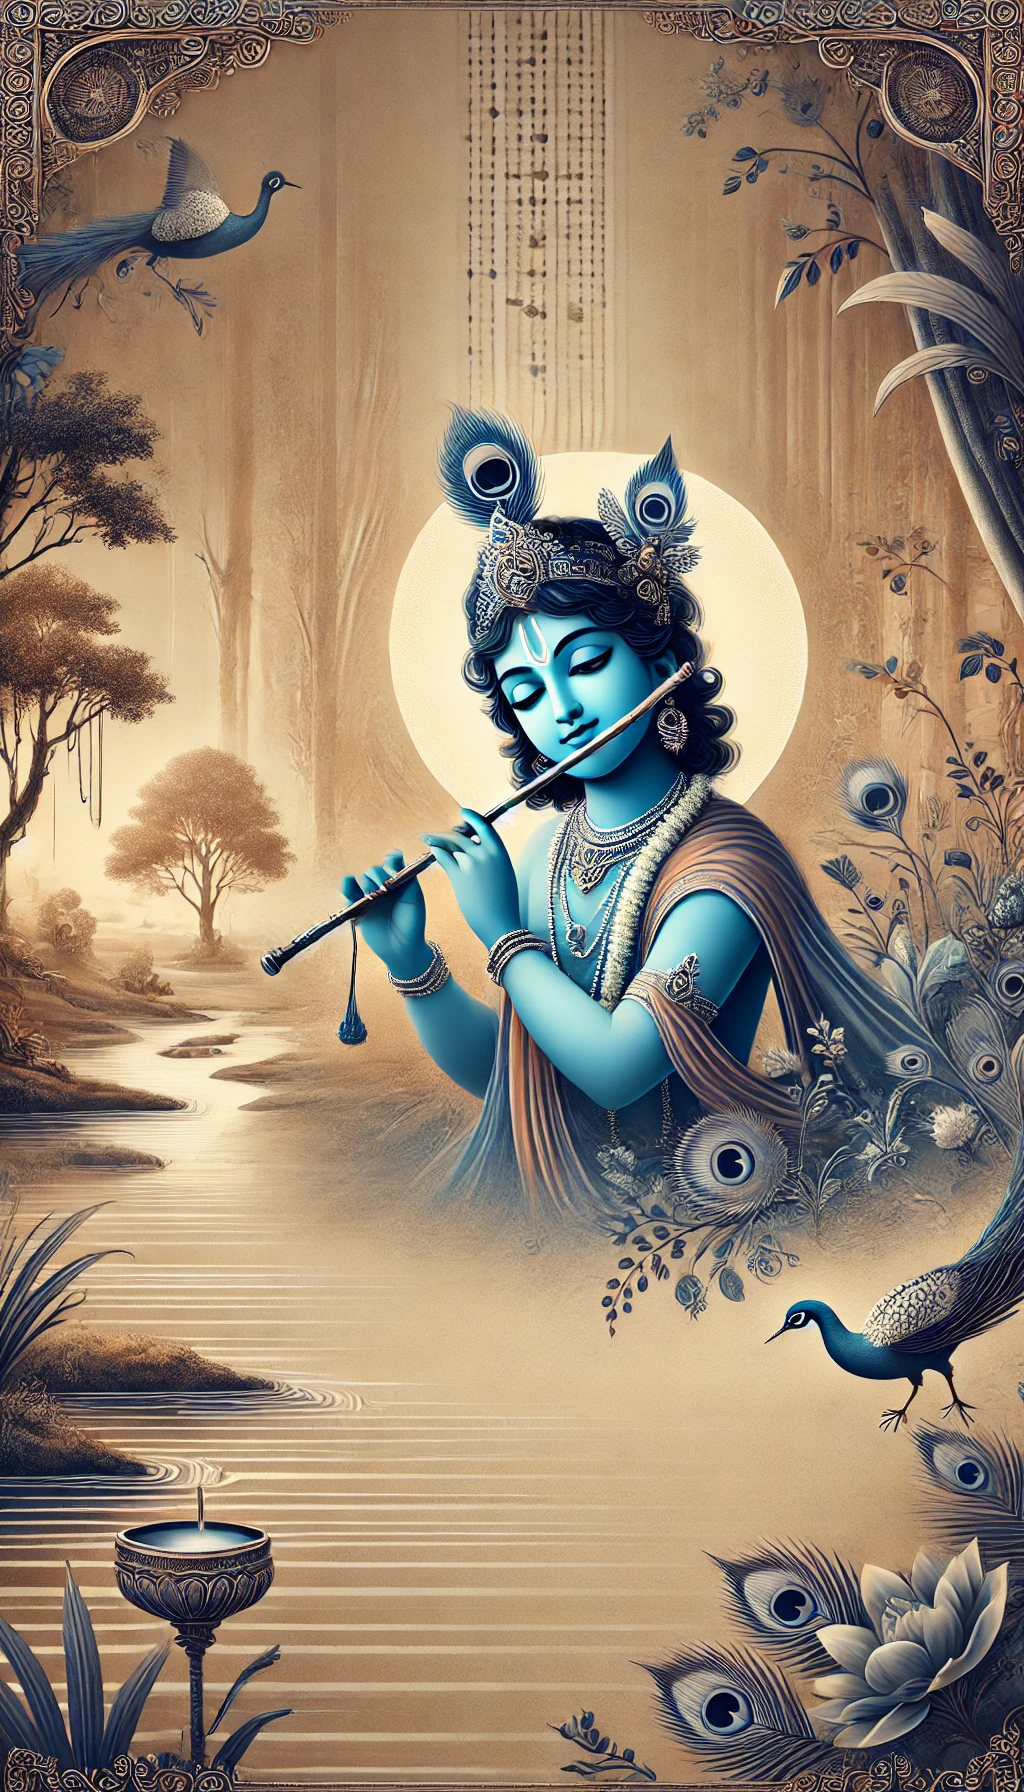
\includegraphics[width=\paperwidth, height=\paperheight, keepaspectratio]{./images/krishna2.png}
\end{center}
\restoregeometry % Restore original geometry settings
\newpage

\begin{mananam}{\mananamfont ಮನನ ಶ್ಲೋಕ - \textenglish{23, 24}}
\footnotesize \mananamtext ನನ್ನ ಬಗ್ಗೆ ನನಗಿರುವ ದೃಷ್ಟಿಕೋನದಂತೆಯೇ ನನ್ನ ನಡವಳಿಕೆ ಜೀವನ ಮತ್ತು ಅದರಾಚೆಗೂ ಇರುತ್ತದೆ. ಸವಾಲುಗಳು, ತೊಂದರೆಗಳು, ನೋವು ಮತ್ತು ಅಂತಿಮವಾಗಿ ಸಾವಿನ ಭಯದಿಂದ ಜೀವನದ ಸನ್ನಿವೇಶಗಳನ್ನು ಎದುರಿಸಲು ನಾನು ಹೆದರುತ್ತೀನೆಯೇ? ಅಥವಾ ನನ್ನ ಮತ್ತು ಇತರರ ಬಗ್ಗೆ ನನ್ನ ದೃಷ್ಟಿಕೋನ ಅಚಲವಾಗಿದೆಯೇ? ನಾನು ನನ್ನ ದೇಹಕ್ಕೆ ಮಾತ್ರ ಸೀಮಿತ ಎಂದು ಗುರುತಿಸಿಕೊಳ್ಳುತ್ತೇನಾ?
\end{mananam}
\WritingHand\enspace\textbf{ಆತ್ಮ ವಿಮರ್ಶೆ}
\begin{inspiration}{\mananamfont ಸ್ಪೂರ್ತಿ}
\footnotesize \mananamtext ಸ್ಥೂಲ ವಸ್ತುಗಳು ಸ್ಥೂಲ ಅಂಶಗಳ ಮೇಲೆ ಪರಿಣಾಮ ಬೀರಬಹುದು ಆದರೆ ಸೂಕ್ಷ್ಮಅಂಶಗಳಿಗಲ್ಲ. ಹಾದು ಹೋಗುವ ಗಾಳಿ ಅಥವಾ ಬೆಂಕಿಯು ಆಕಾಶದ ಮೇಲೆ ಯಾವುದೇ ಪರಿಣಾಮ ಬೀರುವುದಿಲ್ಲ. ದೈಹಿಕ ಅಥವಾ ಮಾನಸಿಕ ರೂಪಾಂತರಗಳಿಂದ ಆತ್ಮಕ್ಕೆ ಏನೂ ಪರಿಣಾಮವಾಗುವುದಿಲ್ಲ.
\end{inspiration}
\newpage

\begin{mananam}{\mananamfont ಮನನ ಶ್ಲೋಕ - \textenglish{27}}
\footnotesize \mananamtext ವಯಸ್ಸಾಗುತ್ತಿರುವುದು ನನಗೆ ಭಯ ಉಂಟು ಮಾಡುತ್ತಿದೆಯಾ? ಬದಲಾವಣೆಗಳು ನನಗೆ ಆತಂಕ ತರುತ್ತಿದೆಯಾ? ಜೀವನದ ಬದಲಾವಣೆಗಳನ್ನು ನಾನು ಶಾಂತ ರೀತಿಯಿಂದ ಸ್ವೀಕರಿಸಬಹುದೇ? ಬದಲಾಗುತ್ತಿರುವ ಈ ದೇಹದ ಲಕ್ಷಣ ಮತ್ತು ಸುತ್ತಲಿನ ಪರಿಸರದ ಬದಲಾವಣೆಗೆ ನಾನು ಸ್ವೀಕಾರ ಮನೋಭಾವ ತರಬಹುದಾ? 
\end{mananam}
\WritingHand\enspace\textbf{ಆತ್ಮ ವಿಮರ್ಶೆ}
\begin{inspiration}{\mananamfont ಸ್ಪೂರ್ತಿ}
\footnotesize \mananamtext ಈ ಸಮಯವೂ ಕಳೆದು ಹೋಗವುದು ಎಂದು ಒಂದು ಪುರಾತನ ಗಾದೆ ಇದೆ. ಒಳ್ಳೆಯ ಸಮಯಗಳಲ್ಲಾಗಲಿ ಅಥವಾ ಕಷ್ಟದ ಸಮಯದಲ್ಲಾಗಲಿ, ಈ ಗಾದೆಯನ್ನು ಅಳಪಡಿಸಿಕೊಳ್ಳುವುದರಿಂದ ನಮ್ಮಲ್ಲಿ ಸ್ವೀಕಾರ ಮನೋಭಾವ ಮತ್ತು ಎಲ್ಲವೂ ಒಳ್ಳೆಯದಾಗುವುದು ಎಂಬ ಮನೋಭಾವ ಉಂಟಾಗುವುದು.
\end{inspiration}
\newpage

\slcol{\Index{ಆಶ್ಚರ್ಯವತ್ಪಶ್ಯತಿ ಕಶ್ಚಿದೇನ}ಮಾಶ್ಚರ್ಯ-\\ವದ್ವದತಿ ತಥೈವ ಚಾನ್ಯಃ ।\\
ಆಶ್ಚರ್ಯವಚ್ಚೈನಮನ್ಯಃ ಶೃಣೋತಿ \\ಶ್ರುತ್ವಾಪ್ಯೇನಂ ವೇದ ನ ಚೈವ ಕಶ್ಚಿತ್ ॥ 29 ॥}
\cquote{ಈ ಆತ್ಮನನ್ನು ಒಬ್ಬಾನೊಬ್ಬನು ಆಶ್ಚರ್ಯವಾಗಿ ನೋಡುತ್ತಾನೆ. ಮತ್ತೊಬ್ಬನು ಆಶ್ಚರ್ಯವಾಗಿ ಹೇಳುತ್ತಾನೆ. ಮತ್ತೊಬ್ಬನು ಆಶ್ಚರ್ಯವಾಗಿ ಕೇಳುತ್ತಾನೆ. ಕೇಳಿದರೂ ಈ ಆತ್ಮನನ್ನು ಯಾರೂ ತಿಳಿಯಲಾರರು.\\}
\slcol{\Index{ದೇಹೀ ನಿತ್ಯಮವಧ್ಯೋऽಯಂ} ದೇಹೇऽಸರ್ವಸ್ಯ ಭಾರತ ।\\
ತಸ್ಮಾತ್ಸರ್ವಾಣಿ ಭೂತಾನಿ ನ ತ್ವಂ ಶೋಚಿತುಮರ್ಹಸಿ ॥ 30 ॥}
\cquote{ಅರ್ಜುನ, ಎಲ್ಲರ ದೇಹದಲ್ಲಿರುವ ಈ ಆತ್ಮ ತತ್ವ ಕೊಲ್ಲಬರುವಂಥ ವಸ್ತುವಲ್ಲ. ಆದ್ದರಿಂದ ಯಾವ ಪ್ರಾಣಿಯ ಬಗೆಗೂ ನೀನು ವ್ಯಥೆಪಡುವ ಕಾರಣವಿಲ್ಲ.\\}
\slcol{\Index{ಸ್ವಧರ್ಮಮಪಿ ಚಾವೇಕ್ಷ್ಯ} ನ ವಿಕಂಪಿತುಮರ್ಹಸಿ ।\\
ಧರ್ಮ್ಯಾದ್ಧಿ ಯುದ್ಧಾಚ್ಛ್ರೇಯೋऽನ್ಯತ್ಕ್ಷತ್ರಿಯಸ್ಯ ನ ವಿದ್ಯತೇ ॥ 31 ॥}
\cquote{ಯುದ್ಧವು ನಿನ್ನ ಸಹಜ ಧರ್ಮವೆಂಬುದನ್ನು ನೋಡಿಯಾದರೂ ನೀನು ಕಂಗೆಡಬಾರದು. ಕ್ಷತ್ರಿಯನಿಗೆ ಧರ್ಮಯುದ್ಧಕ್ಕಿಂತ ಬೇರೆ ಶ್ರೇಯಸ್ ಇಲ್ಲ.\\}
\slcol{\Index{ಯದೃಚ್ಛಯಾ ಚೋಪಪನ್ನಂ} ಸ್ವರ್ಗದ್ವಾರಮಪಾವೃತಮ್ ।\\
ಸುಖಿನಃ ಕ್ಷತ್ರಿಯಾಃ ಪಾರ್ಥ ಲಭಂತೇ ಯುದ್ಧಮೀದೃಶಮ್ ॥ 32 ॥}
\cquote{ಅರ್ಜುನ, ತಾನಾಗಿ ಒದಗಿ ಬಂದ ಇಂತಹ ಯುದ್ಧವೆಂದರೆ ತೆರೆದಿಟ್ಟ ಸ್ವರ್ಗದ ಬಾಗಿಲು. ಇಂಥ ಯುದ್ಧವನ್ನು ಪುಣ್ಯಶಾಲಿಗಳಾದ ಕ್ಷತ್ರಿಯರು ಪಡೆಯುತ್ತಾರೆ.\\}
\slcol{\Index{ಅಥ ಚೇತ್ತ್ವಮಿಮಂ ಧರ್ಮ್ಯಂ} ಸಂಗ್ರಾಮಂ ನ ಕರಿಷ್ಯಸಿ ।\\
ತತಃ ಸ್ವಧರ್ಮಂ ಕೀರ್ತಿಂ ಚ ಹಿತ್ವಾ ಪಾಪಮವಾಪ್ಸ್ಯಸಿ ॥ 33 ॥}
\cquote{ನೀನು ಈ ಧರ್ಮ ಯುದ್ಧವನ್ನು ಮಾಡದೆ ಬಿಟ್ಟರೆ ಸ್ವಧರ್ಮಭ್ರಷ್ಟನೂ ಕೀರ್ತಿಭ್ರಷ್ಟನೂ ಆಗಿ ಪಾಪಕ್ಕೆ ಗುರಿಯಾಗುವೆ.\\}
\slcol{\Index{ಅಕೀರ್ತಿಂ ಚಾಪಿ ಭೂತಾನಿ} ಕಥಯಿಷ್ಯಂತಿ ತೇऽವ್ಯಯಾಮ್ ।\\
ಸಂಭಾವಿತಸ್ಯ ಚಾಕೀರ್ತಿರ್ಮರಣಾದತಿರಿಚ್ಯತೇ ॥ 34 ॥}
\cquote{ನಿನ್ನ ಅಪಕೀರ್ತಿಯನ್ನು ಜನರು ಅನಂತಕಾಲದ ವರೆಗೆ ಆಡಿಕೊಳ್ಳುತ್ತಾರೆ. ಮರ್ಯಾದಸ್ತನಿಗೆ ಅಪನಿಂದನೆಯು ಮರಣಕ್ಕಿಂತ ಕೀಳಾದದ್ದು.\\}
\slcol{\Index{ಭಯಾದ್ರಣಾದುಪರತಂ} ಮಂಸ್ಯಂತೇ ತ್ವಾಂ ಮಹಾರಥಾಃ ।\\
ಯೇಷಾಂ ಚ ತ್ವಂ ಬಹುಮತೋ ಭೂತ್ವಾ ಯಾಸ್ಯಸಿ ಲಾಘವಮ್ ॥ 35 ॥}
\cquote{ನಿನ್ನನ್ನು, ಭಯದಿಂದ ಯುದ್ಧವನ್ನು ಬಿಟ್ಟವನೆಂದು ಈ ಕ್ಷತ್ರಿಯ ವೀರರು ತಿಳಿಯುತ್ತಾರೆ. ಇಲ್ಲಿಯವರೆಗೆ ನಿನ್ನನ್ನು ಗೌರವದಿಂದ ನೋಡಿದವರೇ ಈಗ ಹಗುರಾಗಿ ನೋಡುವರು.}

\begin{mananam}{\mananamfont ಮನನ ಶ್ಲೋಕ - \textenglish{29}}
\footnotesize \mananamtext ನಾನು ನಮ್ಮ ಜೀವನವನ್ನು ಹೊಸ ದೃಷ್ಟಿಕೋನದಿಂದ ನೋಡಬಹುದಾ? ನಾನು ಪಕ್ಷಪಾತಿಯಾಗಿದ್ದೀನಾ? ಎಲ್ಲದರ ಬಗ್ಗೆ ವಿಮರ್ಶಾತ್ಮಕವಾಗಿ ನಿರ್ಣಯ ತೆಗೆದುಕೊಳ್ಳುತ್ತೇನಾ? ನನ್ನ ಈ ಕ್ಷಣದ ಅನುಭವಕ್ಕೂ ಹಳೆಯ  ವಿಮರ್ಶಾತ್ಮಕ ಬಣ್ಣ ಬಳೆಯುತ್ತೀನಾ?
\end{mananam}
\WritingHand\enspace\textbf{ಆತ್ಮ ವಿಮರ್ಶೆ}
\begin{inspiration}{\mananamfont ಸ್ಪೂರ್ತಿ}
\footnotesize \mananamtext ಮಗು ಎಲ್ಲವನ್ನೂ ಆಶ್ಚರ್ಯ ಮತ್ತು ಕುತೂಹಲದಿಂದ ನೋಡುತ್ತದೆ. ಅದು ಎಲ್ಲವನ್ನು ಹೊಸತನ, ತಾಜಾತನ ಮತ್ತು ಸಂತೋಷದಿಂದ ಅನುಭವಿಸುತ್ತದೆ. ಆದರೆ ಅದು ಬೆಳೆದಂತೆ ತಾನು ಏನನ್ನು ಮಾಡಬೇಕು, ಕೇಳಬೇಕು ಎಂದು ಬಯಸುವ ಕಡೆಗೆ ಪಕ್ಷಪಾತ ಭಾವನೆ ಬೆಳೆಸಿಕೊಳ್ಳುವುದು. ಅನಂತರ ಶೀಘ್ರದಲ್ಲಿಯೇ ಜೀವನವು ಬೇಸರ, ಮಂದ ನಿರಾಶದಾಯಕವಾಗುತ್ತದೆ. ನಿಮ್ಮೊಳಗಿನ ಮಗುವನ್ನು ಪುನರ್ಜೀವಗೊಳಿಸಿ. ಜೀವನದ ಪ್ರತಿ ಕ್ಷಣವನ್ನು ತಾಜಾತನ ಮತ್ತು ನಿಷ್ಕಲ್ಮಶ ಮನಸ್ಸಿನಿಂದ ಅನುಭವಿಸಿ.
\end{inspiration}
\newpage

\begin{mananam}{\mananamfont ಮನನ ಶ್ಲೋಕ - \textenglish{31}}
\footnotesize \mananamtext ನನ್ನ ಜೀವನದಲ್ಲಿ ಅನ್ಯಾಯವಾಗಿ ನನ್ನ ಮೇಲೆ ಕೆಲವು ಕರ್ತವ್ಯಗಳು ಹೇರಲಾಗಿದೆ ಎಂದು ಭಾವಿಸುತ್ತೇನಾ? ಆದರೆ ಈ ಕರ್ತವ್ಯಗಳನ್ನು ನಿಭಾಯಿಸಲು ಕಲಿತರೆ ನನ್ನ ಜೀವನ ಪ್ರಕಾಶಮಯವಾಗಬಹುದಾ? ನನ್ನ ಜೀವನದಲ್ಲಿ ಬರುವ ಕರ್ತವ್ಯಗಳನ್ನು ಗೊಣಗದೆ, ದೂರದೆ, ಸಂಪೂರ್ಣ ಸ್ವೀಕಾರ ಮನೋಭಾವದಿಂದ ಮಾಡಲು ಕಲಿತರೆ ಒಳ್ಳೆಯದಲ್ಲವೇ?
\end{mananam}
\WritingHand\enspace\textbf{ಆತ್ಮ ವಿಮರ್ಶೆ}
\begin{inspiration}{\mananamfont ಸ್ಪೂರ್ತಿ}
\footnotesize \mananamtext ನಮಗೆ ಇಷ್ಟವಾಗದ ಕರ್ತವ್ಯಗಳು ನಮಗೆ ಕೆಲವು ಅವಕಾಶಗಳು ಮತ್ತು ಕೌಶಲಗಳೊಂದಿಗೆ ಸಜ್ಜುಗೊಳಿಸುತ್ತದೆ. ಪ್ರಕೃತಿಯ ನಿಯಮವೆಂದರೆ ಎಂದಿಗೂ ಯಾರಿಗೂ ಅನ್ಯಾಯವಾಗುವುದಿಲ್ಲ ಮತ್ತು ನಮ್ಮ ಯಾವುದೇ ಪ್ರಯತ್ನಕ್ಕೆ ಪ್ರತಿಫಲ ದೊರಕದೇ ಇರುವುದಿಲ್ಲ.
\end{inspiration}
\newpage

\begin{mananam}{\mananamfont ಮನನ ಶ್ಲೋಕ - \textenglish{33}}
\footnotesize \mananamtext ಈಗಿನ ಪರಿಸ್ಥಿತಿಯಲ್ಲಿ ನನ್ನ ಸ್ವಧರ್ಮ ಯಾವುದು? ಬದಲಾಗುತ್ತಿರುವ ಕಾಲದಲ್ಲಿ ನಾನು ನನ್ನ ಧರ್ಮವನ್ನು ಹೇಗೆ ಅಳವಡಿಸಿಕೊಳ್ಳಲಿ? ಸಮಾಜದಲ್ಲಿ ಆತ್ಮಗೌರವ ಮತ್ತು ಘನತೆಯನ್ನು ಕಾಪಾಡಿಕೊಳ್ಳಲು ನಾನು ಹೇಗೆ ವರ್ತಿಸಬೇಕು? ನಾನು ಎತ್ತಿ ಹಿಡಿಯಬೇಕಾದ ಯಾವುದೇ ಕರ್ತವ್ಯಗಳು ಅಥವಾ ಮೌಲ್ಯಗಳನ್ನು ತ್ಯಜಿಸುತ್ತಿದ್ದೇನೆಯೇ? ನಾನು ನನ್ನ ಜೀವನದ ಯುದ್ಧವನ್ನು ಎದುರಿಸಲು ಭಯಪಡುತ್ತೇನಾ?
\end{mananam}
\WritingHand\enspace\textbf{ಆತ್ಮ ವಿಮರ್ಶೆ}
\begin{inspiration}{\mananamfont ಸ್ಪೂರ್ತಿ}
\footnotesize \mananamtext ಪರಮಸತ್ಯವನ್ನು ಪಡೆಯಲು ಪೂರ್ಣ ಹೃದಯದಿಂದ ಬದ್ಧನಾಗಿರುವವನು ತ್ಯಾಗ ಮಾಡಿದರೆ ಸ್ವೀಕಾರಾರ್ಹವಾಗುವುದು. ಒಬ್ಬನು ತನ್ನ ರಾಷ್ಟ್ರಕ್ಕೋಸ್ಕರ ಅಥವಾ ಒಂದು ದೊಡ್ಡ ಸಮುದಾಯಕೋಸ್ಕರ ಸೇವೆ ಸಲ್ಲಿಸುವುದರಲ್ಲಿ ನಿರತನಾಗಿದ್ದಕ್ಕೆ ತನ್ನ ಕುಟುಂಬದ ಜವಾಬ್ದಾರಿಯನ್ನು ಹೊರಲು ವಿಫಲನಾದರೆ ಇದು ಸ್ವೀಕಾರಾರ್ಹವಾಗಿದೆ. ಆದರೆ ಸೋಮಾರಿತನ, ತನ್ನ ಆಕಾಂಕ್ಷೆಗೋಸ್ಕರ ಮತ್ತು ನಕರಾತ್ಮಕತೆ ಮತ್ತು ಭಯದಿಂದ ಹೊರಬರಲು ತನ್ನ ಕುಟುಂಬ, ಸಮಾಜದಿಂದ ಆತ್ಮಕ್ಕೆ ಕರ್ತವ್ಯ ಮತ್ತು ಜವಾಬ್ದಾರಿ ಯನ್ನು ತ್ಯಜಿಸುವುದು ತನಗೂ ಮತ್ತು ಬೇರೆಯವರಿಗೂ ಮಾಡುವ ಅತ್ಯಂತ ಕೆಟ್ಟ ಕೆಲಸ ವಾಗುವುದು.
\end{inspiration}
\newpage


\slcol{\Index{ಅವಾಚ್ಯವಾದಾಂಶ್ಚ ಬಹೂನ್ವ}ದಿಷ್ಯಂತಿ ತವಾಹಿತಾಃ ।\\
ನಿಂದಂತಸ್ತವ ಸಾಮರ್ಥ್ಯಂ ತತೋ ದುಃಖತರಂ ನು ಕಿಮ್ ॥ 36 ॥}
\cquote{ಶತ್ರುಗಳು ನಿನ್ನ ಪರಾಕ್ರಮವನ್ನು ನಿಂದಿಸಿ ಮಾತನಾಡುವರು. ಇದಕ್ಕಿಂತ ಹೆಚ್ಚಿನ ದುಃಖ ಯಾವುದು?\\}
\slcol{\Index{ಹತೋ ವಾ ಪ್ರಾಪ್ಸ್ಯಸಿ} ಸ್ವರ್ಗಂ ಜಿತ್ವಾ ವಾ ಭೋಕ್ಷ್ಯಸೇ ಮಹೀಮ್ ।\\
ತಸ್ಮಾದುತ್ತಿಷ್ಠ ಕೌಂತೇಯ ಯುದ್ಧಾಯ ಕೃತನಿಶ್ಚಯಃ ॥ 37 ॥}
\cquote{ಸತ್ತರೆ ಸ್ವರ್ಗವನ್ನು ಸೇರುವೆ, ಗೆದ್ದರೆ ಭೂಮಿಯನ್ನು ಆಳುವೆ. ಆದ್ದರಿಂದ ಅರ್ಜುನ ಕಾದುವುದಕ್ಕೆ ಮನಸ್ಸು ಗಟ್ಟಿಮಾಡಿಕೊಂಡು ಏಳು.\\}
\slcol{\Index{ಸುಖದುಃಖೇ ಸಮೇ ಕೃತ್ವಾ} ಲಾಭಾಲಾಭೌ ಜಯಾಜಯೌ ।\\
ತತೋ ಯುದ್ಧಾಯ ಯುಜ್ಯಸ್ವ ನೈವಂ ಪಾಪಮವಾಪ್ಸ್ಯಸಿ ॥ 38 ॥}
\cquote{ಸುಖದುಃಖಗಳನ್ನು, ಲಾಭನಷ್ಟಗಳನ್ನು, ಜಯಾಪಜಯಗಳನ್ನು ಸಮನವಾಗಿ ತಿಳಿದು ಯುದ್ಧವನ್ನು ಮಾಡು. ಹಾಗಾದರೆ ಪಾಪಗಳು ನಿನ್ನನ್ನು ಅಂಟಲಾರವು.\\}
\slcol{\Index{ಏಷಾ ತೇऽಭಿಹಿತಾ ಸಾಂಖ್ಯೇ} ಬುದ್ಧಿರ್ಯೋಗೇ ತ್ವಿಮಾಂ ಶೃಣು ।\\
ಬುದ್ಧ್ಯಾ ಯುಕ್ತೋ ಯಯಾ ಪಾರ್ಥ ಕರ್ಮಬಂಧಂ ಪ್ರಹಾಸ್ಯಸಿ ॥ 39 ॥}
\cquote{ಅರ್ಜುನ, ಆತ್ಮನ ವಿಚಾರವಾಗಿ ಈ ತಿಳುವಳಿಕೆಯನ್ನು ನಿನಗೆ ಹೇಳಿದ್ದಾಯಿತು ಈಗ ಅದರ ಉಪಾಯದ ಬಗ್ಗೆ ಕೇಳು. ಅರ್ಜುನ ನೀನು ಇದನ್ನು ತಿಳಿಯುವುದರಿಂದ ಕರ್ಮದ ಕಟ್ಟನ್ನು ಕಳಚಿಕೊಳ್ಳುತ್ತಿ.\\}
\slcol{\Index{ನೇಹಾಭಿಕ್ರಮನಾಶೋऽಸ್ತಿ} ಪ್ರತ್ಯವಾಯೋ ನ ವಿದ್ಯತೇ ।\\
ಸ್ವಲ್ಪಮಪ್ಯಸ್ಯ ಧರ್ಮಸ್ಯ ತ್ರಾಯತೇ ಮಹತೋ ಭಯಾತ್ ॥ 40 ॥}
\cquote{ಇದರ ಆರಂಭ ಮಾತ್ರವೂ ವ್ಯರ್ಥವಲ್ಲ. ಇದರಲ್ಲಿ ದೋಷ ಉಂಟಾಗುವುದಿಲ್ಲ. ಈ ಧರ್ಮದ ಅಲ್ಪಾಚರಣೆ ಕೂಡ ಹಿರಿಯ ಪಾತಕದಿಂದ ಪಾರು ಮಾಡುತ್ತದೆ.\\}
\slcol{\Index{ವ್ಯವಸಾಯಾತ್ಮಿಕಾ ಬುದ್ಧಿ}ರೇಕೇಹ ಕುರುನಂದನ ।\\
ಬಹುಶಾಖಾ ಹ್ಯನಂತಾಶ್ಚ ಬುದ್ಧಯೋऽವ್ಯವಸಾಯಿನಾಮ್ ॥ 41 ॥}
\cquote{ಅರ್ಜುನ, ಈ ಸಾಧನಗಳಲ್ಲಿ ನೆಲೆಗೆ ನಿಂತ ಬುದ್ಧಿಯು ಒಂದೇ ಮುಖವಾಗಿರುವುದು. ನೆಲೆಗೆ ನಿಲ್ಲದವರ ಬುದ್ಧಿಯು ಅನೇಕ ಕೊಂಬೆಗಳುಳ್ಳದಾಗಿ ಬಗೆ ಬಗೆಯಾಗಿರುವುದು. \\}
\slcol{\Index{ಯಾಮಿಮಾಂ ಪುಷ್ಪಿತಾಂ} ವಾಚಂ ಪ್ರವದಂತ್ಯವಿಪಶ್ಚಿತಃ ।\\
ವೇದವಾದರತಾಃ ಪಾರ್ಥ ನಾನ್ಯದಸ್ತೀತಿ ವಾದಿನಃ ॥ 42 ॥}
\cquote{ಅರ್ಜುನ, ದಡ್ಡರು ವೇದದ ಮೇಲ್ನೋಟಕ್ಕೆ ಕಾಣುವ ಹೂವಿನಂತ ಮಾತಿಗೆ ಮರುಳಾಗುತ್ತಾರೆ. ಅದರ ಆಚೆಗಿರುವ ಭಗವತತ್ವವೆಂಬ ಹಣ್ಣು ಅವರಿಗೆ ಕಾಣಿಸದು. ಅದಕ್ಕೆಂದೇ ಅವರು ಅದನ್ನು ನಿರಾಕರಿಸಿಬಿಡುತ್ತಾರೆ.\\}

\newpage
\begin{mananam}{\mananamfont ಮನನ ಶ್ಲೋಕ - \textenglish{38}}
\footnotesize \mananamtext ಜೀವನದಲ್ಲಿ ನಾನು ಎದುರಿಸುವ ಯಾವುದೇ ಸವಾಲಿನ ಬಗ್ಗೆ ನನ್ನ ವರ್ತನೆ ಏನು? ನಾನು ಯಾವುದೇ ತರಹದ ಫಲಿತಾಂಶದ ಕಡೆಗೆ ಸಮಚಿತ್ತನಾಗಿದ್ದೇನೆಯೇ? ನನ್ನ ಅತ್ಯುತ್ತಮ ಪ್ರಯತ್ನದ ಹೊರತಾಗಿಯೂ ಒಳ್ಳೆಯ ಫಲಿತಾಂಶ ಬಂದಾಗ ಅದರ ಬಗ್ಗೆ ಮೋಹವು ಮತ್ತು ಫಲಿತಾಂಶಗಳಿಗೆ ಮಾನಸಿಕವಾಗಿ ವಿಮುಕನಾಗಿದ್ದೇನೆಯೇ? ಗೆಲುವನ್ನು ಬಯಸದೆ ಸೋಲನ್ನು ತಿರಸ್ಕರಿದೆ ಲಾಭವನ್ನು ಹುಡುಕುವ ಮತ್ತು ನಷ್ಟವನ್ನು ತಪ್ಪಿಸುವ ಪ್ರೇರಣೆ ಇಲ್ಲದೆ ಜೀವನದಲ್ಲಿ  ಕಾರ್ಯನಿರ್ವಹಿಸಲು ಕಲಿಯಬಹುದೇ?
\end{mananam}
\WritingHand\enspace\textbf{ಆತ್ಮ ವಿಮರ್ಶೆ}
\begin{inspiration}{\mananamfont ಸ್ಪೂರ್ತಿ}
\footnotesize \mananamtext ಯಾವಾಗಲೂ ಗೆಲುವನ್ನು ಬಯಸುವುದು ಮತ್ತು ಸಂತೋಷವಾಗಿರಲು ಬಯಸುವುದು ಎಲ್ಲರಲ್ಲಿ ಸಹಜವಾಗಿರುವ ಒಲವು. ಹಾಗೆಯೇ ಅಹಿತಕರವಾದದ್ದನ್ನು ತಪ್ಪಿಸುವುದು ಮತ್ತು ಎಂದಿಗೂ ಸೋಲನ್ನು ಬಯಸದೇ ಇರುವುದು ಪ್ರವೃತ್ತಿಯಾಗಿದೆ. ಆದರೆ ನಿಜವಾದ ಸ್ವಾತಂತ್ರ್ಯ ಹೊಂದಿದ ವ್ಯಕ್ತಿಗೆ ಎಲ್ಲಾ ಕ್ರಿಯೆಗಳು ನೀರಿನಲ್ಲಿ ರೇಖೆಯನ್ನು ಎಳೆಯುವಂತಿದೆ. ಅವನು ಮಾನಸಿಕವಾಗಿ ಕಳಂಕರಹಿತ ಮತ್ತು ಯಾವುದೇ ತರಹದ ಕರ್ಮವು ಅವನನ್ನು ಬಂಧಿಸುವುದಿಲ್ಲ.
\end{inspiration}
\newpage


\slcol{\Index{ಕಾಮಾತ್ಮಾನಃ ಸ್ವರ್ಗಪರಾ} ಜನ್ಮಕರ್ಮಫಲಪ್ರದಾಮ್ ।\\
ಕ್ರಿಯಾವಿಶೇಷಬಹುಲಾಂ ಭೋಗೈಶ್ವರ್ಯಗತಿಂ ಪ್ರತಿ ॥ 43 ॥}
\cquote{ಅವರು ಬಯಕೆಯ ಬೆನ್ನು ಹತ್ತಿದವರು. ಸ್ವರ್ಗವೇ ಪುರುಷಾರ್ಥ ಎಂದು ಭ್ರಮಿಸಿದವರು. ನಮ್ಮನ್ನು ಹುಟ್ಟು ಸಾವುಗಳ ಸುಳಿಯಲ್ಲಿ ಸಿಕ್ಕಿಸುವ ಕರ್ಮಕಾಂಡದ ಕ್ಷಣಿಕ ಭೋಗಭಾಗ್ಯಗಳಿಗೆ ಮರುಳಾದವರು.\\}
\slcol{\Index{ಭೋಗೈಶ್ವರ್ಯಪ್ರಸಕ್ತಾನಾಂ} ತಯಾಪಹೃತಚೇತಸಾಮ್ ।\\
ವ್ಯವಸಾಯಾತ್ಮಿಕಾ ಬುದ್ಧಿಃ ಸಮಾಧೌ ನ ವಿಧೀಯತೇ ॥ 44 ॥}
\cquote{ಇಂದ್ರಿಯ ಭೋಗ ಮತ್ತು ಸಂಪತ್ತುಗಳಲ್ಲಿ ಆಸಕ್ತರಾದ ಇಂಥವರು ಫಲಸ್ತುತಿಗಳ (ಹೊಗಳಿಕೆಯ) ಮಾತಿನ ಸೆಳೆತಕ್ಕೆ ಮರುಳಾಗುತ್ತಾರೆ. ಅಂತವರ ಮನಸ್ಸಿನಲ್ಲಿ ನೆಲೆ ನಿಂತ ತತ್ವದ ತಿಳುವಳಿಕೆ ಉಂಟಾಗುವುದಿಲ್ಲ.\\}
\slcol{\Index{ತ್ರೈಗುಣ್ಯವಿಷಯಾ ವೇದಾ} ನಿಸ್ತ್ರೈಗುಣ್ಯೋ ಭವಾರ್ಜುನ ।\\
ನಿರ್ದ್ವಂದ್ವೋ ನಿತ್ಯಸತ್ತ್ವಸ್ಥೋ ನಿರ್ಯೋಗಕ್ಷೇಮ ಆತ್ಮವಾನ್ ॥ 45 ॥}
\cquote{ಅರ್ಜುನಾ, ವೇದಗಳು ತ್ರಿಗುಣ ರೂಪವಾದ ಸಂಸಾರವನ್ನು ಹೇಳುತ್ತವೆ. ನೀನು ತ್ರಿಗುಣಾತೀತನು ದ್ವಂದ್ವರಹಿತನು ಆಗು. ಶುದ್ಧ ಸತ್ವವನ್ನು ಆಶ್ರಯಿಸುವವನಾಗಿಯೂ ಯೋಗ ಕ್ಷೇಮಗಳ ಚಿಂತೆ ಇಲ್ಲದವನಾಗಿ  ಆಗು. ಆತ್ಮನಿಷ್ಟನಾಗಿರು.\\}
\slcol{\Index{ಯಾವಾನರ್ಥ ಉದಪಾನೇ} ಸರ್ವತಃ ಸಂಪ್ಲುತೋದಕೇ ।\\
ತಾವಾನ್ಸರ್ವೇಷು ವೇದೇಷು ಬ್ರಾಹ್ಮಣಸ್ಯ ವಿಜಾನತಃ ॥ 46 ॥}
\cquote{ಭಾವಿಯಿಂದ ಆಗುವ ಪ್ರಯೋಜನ ಎಲ್ಲೆಡೆಯೂ ತುಂಬಿ ಹರಿಯುವ ಸಮುದ್ರದಿಂದ ಆಗಿಯೇ ಆಗುತ್ತದೆ. ಹಾಗೆಯೇ ವೇದದಲ್ಲಿ ಹೇಳಿರುವ ಎಲ್ಲಾ ಫಲಗಳು ಬ್ರಹ್ಮ ಜ್ಞಾನಿಗೆ ಸಿಕ್ಕೇ ಸಿಗುವುದು.\\}
\slcol{\Index{ಕರ್ಮಣ್ಯೇವಾಧಿಕಾರಸ್ತೇ ಮಾ} ಫಲೇಷು ಕದಾಚನ ।\\
ಮಾ ಕರ್ಮಫಲಹೇತುರ್ಭೂರ್ಮಾ ತೇ ಸಂಗೋऽಸ್ತ್ವಕರ್ಮಣಿ ॥ 47 ॥}
\cquote{ಕರ್ಮ ಮಾಡುವುದಷ್ಟೇ ನಿನ್ನ ಹಕ್ಕು. ಕರ್ಮಫಲದ ಮೇಲೆ ಹಕ್ಕು ಸಾಧಿಸಬೇಡ. ಫಲದ ಆಸೆಯಿಂದ ಕರ್ಮ ಮಾಡಲು ಬೇಡ. ಹಾಗೆಯೇ ಕರ್ಮ ತ್ಯಾಗದ ಕಡೆಗೂ ನಿನ್ನ ಒಲವು ಹರಿಯದಿರಲಿ.\\}
\slcol{\Index{ಯೋಗಸ್ಥಃ ಕುರು ಕರ್ಮಾಣಿ} ಸಂಗಂ ತ್ಯಕ್ತ್ವಾ ಧನಂಜಯ ।\\
ಸಿದ್ಧ್ಯಸಿದ್ಧ್ಯೋಃ ಸಮೋ ಭೂತ್ವಾ ಸಮತ್ವಂ ಯೋಗ ಉಚ್ಯತೇ ॥ 48 ॥}
\cquote{ಅರ್ಜುನ, ಯೋಗ ನಿಷ್ಠನಾಗಿ ಫಲಕ್ಕಾಗಿ ಆಸೆ ಮಾಡದೆ ಫಲ ದೊರೆತರೆ ಹಿಗ್ಗದೆ ಸಿಗದಿದ್ದರೆ ಕುಗ್ಗದೇ ಒಂದೇ ಭಾವದಿಂದ ಕರ್ಮವನ್ನು ಮಾಡು. ಈ ಸಮದೃಷ್ಟಿಯೇ ನಿಜವಾದ ಯೋಗ.\\}

\clearpage
\newgeometry{margin=0pt} % Apply margin only for this page
\thispagestyle{empty}
\begin{center}
\includegraphics[width=\paperwidth, height=\paperheight, keepaspectratio]{./images/krishna1.png}
\end{center}
\restoregeometry % Restore original geometry settings
\newpage

\begin{mananam}{\mananamfont ಮನನ ಶ್ಲೋಕ - \textenglish{45}}
\footnotesize \mananamtext ಒಳ್ಳೆಯದು, ಕೆಟ್ಟದ್ದು, ಸುಂದರ, ಕೊಳಕು, ಬಿಳಿ ಮತ್ತು ಕಪ್ಪು ಈ ಜೋಡಿ ವಿರುದ್ಧ ಪದಗಳಿಂದ ನನ್ನ ಜೀವನದ ದೃಷ್ಟಿಕೋನವು ಕಳಂಕಿತವಾಗಿದೆಯೇ? ನಾನು ಯಾವಾಗಲೂ ಇತರರ ಬಗ್ಗೆ ಮತ್ತು ನನ್ನ ಬಗ್ಗೆ ವಿಮರ್ಶಾತ್ಮಕವಾಗಿದ್ದೇನೆಯೇ? ನನ್ನೊಳಗೆ ಮತ್ತು ಇತರರೊಂದಿಗೆ ಸಂಘರ್ಷದ ಮೂಲವಾಗಿರುವ ವಿಪರೀತ ದೃಷ್ಟಿಕೋನಗಳಿಗೆ ನಾನು ಅಂಟಿಕೊಂಡಿದ್ದೇನೆಯೇ? ಈ ಎಲ್ಲಾ ಅನಿಸಿಕೆಗಳು ಮತ್ತು ವಿಮರ್ಶೆಗಳಿಂದ ಮೇಲೆ ಬರುವಷ್ಟು ಧೈರ್ಯವಿದೆಯೇ? ಎಲ್ಲದರಲ್ಲೂ ತಟಸ್ಥವಾಗಿರದೆ ತೆರೆದ ಮನಸ್ಸು ಮತ್ತು ಸ್ವೀಕಾರ ಮನೋಭಾವದಿಂದ ಹೆಚ್ಚಿನ ಆಯಾಮಕ್ಕೆ ತೆರೆದುಕೊಳ್ಳಬಲ್ಲೆನೇ?
\end{mananam}
\WritingHand\enspace\textbf{ಆತ್ಮ ವಿಮರ್ಶೆ}
\begin{inspiration}{\mananamfont ಸ್ಪೂರ್ತಿ}
\footnotesize \mananamtext ಎಲ್ಲಾ ಒತ್ತಡದ ಮತ್ತು ಆತಂಕಗಳಿಂದ ನಿಮ್ಮನ್ನು ಮುಕ್ತಿಗೊಳಿಸಲು ತಕ್ಷಣದ ಮಾರ್ಗವೆಂದರೆ ನಿಮ್ಮ ದಿನಚರಿಯದಲ್ಲಿ ಕೆಲವು ನಿಮಿಷಗಳ ಕಾಲ ದೇಹಕ್ಕೆ ವಿಶ್ರಾಂತಿ ಕೊಟ್ಟು ಮನಸ್ಸಿಗೆ ಅದರ ನೈಸರ್ಗಿಕ ಸ್ಥಿತಿಯಲ್ಲಿರುವುದು ಅಂದರೆ ಏನನ್ನು ಮಾಡಲು ಬಯಸದೇ ಇರುವುದು ಮತ್ತು ಏನನ್ನು ಮಾಡದೇ ಇರುವುದು. ಈ ಸ್ಥಿತಿಯು ಧ್ಯಾನವೂ ಅಲ್ಲ ಅಥವಾ ನಿದ್ರಿಸುವುದು ಅಲ್ಲ. ಇದು ನಿಮ್ಮ ಆತ್ಮದೊಂದಿಗೆ ನೀವು ಇರುವ ಸ್ಥಿತಿಯು ಸಹಜವು ಮತ್ತು ಆಳವಾಗಿ ತೃಪ್ತವಾಗಿರುವುದಾಗಿದೆ. ಇದು ತ್ರಿಗುಣಗಳಾದ ಸತ್ವ, ರಜಸ್, ತಮಸ್ ನಿಂದ ಮುಕ್ತವಾಗಿದೆ. ಇವು ನಮ್ಮನ್ನು ಯಾವಾಗಲೂ ಹೊರಗೆ ತೊಡಗಿಸಿಟ್ಟುಕೊಂಡಿರುತ್ತದೆ.
\end{inspiration}
\newpage

\newpage
\begin{mananam}{\mananamfont ಮನನ ಶ್ಲೋಕ - \textenglish{47,48}}
\footnotesize \mananamtext ಏನನ್ನಾದರೂ ಮಾಡುವಾಗ ಫಲಿತಾಂಶವನ್ನು ಎದುರು ನೋಡದೆ ಇರುವುದನ್ನು ಹಾಗೂ ಅಹಿತಕರ ಫಲಿತಾಂಶ ಬಂದರೂ ಕೂಡ ಸಮತ್ವ ಸ್ಥಿತಿಯಲ್ಲಿ ಇರಲು ಕಲಿಯಬಹುದೇ? ಹೆಚ್ಚಿನವರಂತೆ ನಾನು ಕೂಡ ಎಲ್ಲ ಸಂಬಂಧಗಳನ್ನು ವ್ಯವಹಾರಿಕ ದೃಷ್ಟಿಕೋನದಿಂದ ನೋಡುತ್ತೇನೆಯೇ? ಯಾರಿಂದಲೂ ಏನನ್ನು ತೆಗೆದುಕೊಳ್ಳಲು ಬಯಸದೆ ನಾನು ಕೊಡುವುದನ್ನು ಮಾತ್ರ ಕಲಿಯಬಹುದೇ? ತೆಗೆದುಕೊಳ್ಳದೆ ಕೊಡುವ ಈ ತತ್ವವನ್ನು ದಿನನಿತ್ಯ ಜೀವನದಲ್ಲಿ ಸಣ್ಣ ವಿಷಯಗಳಿಗೂ ಅಳವಡಿಸಲು ಅಭ್ಯಾಸ ಮಾಡಿಕೊಳ್ಳಬಹುದೇ? ಇದರಿಂದ ಈ ತತ್ವವನ್ನು ನನ್ನ ಜೀವನದಲ್ಲಿ ದೊಡ್ಡ ದೊಡ್ಡ ವಿಷಯಗಳಿಗೆ ಅಳವಡಿಸಿಕೊಳ್ಳಲು ಸಾಧ್ಯವಾಗಬಹುದೇ?
\end{mananam}
\WritingHand\enspace\textbf{ಆತ್ಮ ವಿಮರ್ಶೆ}
\begin{inspiration}{\mananamfont ಸ್ಪೂರ್ತಿ}
\footnotesize \mananamtext ಮನಸ್ಸಿನ ಸಮತ್ವವನ್ನು ಸಾಧಿಸಲು ಎಲ್ಲಾ ನಿರೀಕ್ಷೆಗಳಿಂದ ಮನಸ್ಸನ್ನು ಶುದ್ಧೀಕರಿಸುವುದು ಅತ್ಯಗತ್ಯ. ದಿನನಿತ್ಯದ ಜೀವನದಲ್ಲಿ ಮನಸ್ಸಿನ ಈ ಸಮುತ್ವವನ್ನು ಕಾಪಾಡಿಕೊಳ್ಳುವುದು ಯೋಗ ಮತ್ತು ಈ ಸ್ಥಿತಿಯನ್ನು ಯಾರು ಸಾಧಿಸುತ್ತಾರೋ ಅವನೇ ಯೋಗಿ.
\end{inspiration}
\newpage

\slcol{\Index{ದೂರೇಣ ಹ್ಯವರಂ ಕರ್ಮ} ಬುದ್ಧಿಯೋಗಾದ್ಧನಂಜಯ ।\\
ಬುದ್ಧೌ ಶರಣಮನ್ವಿಚ್ಛ ಕೃಪಣಾಃ ಫಲಹೇತವಃ ॥ 49 ॥}
\cquote{ಅರ್ಜುನ, ಇಂತಹ ಜ್ಞಾನಮಾರ್ಗಕ್ಕಿಂತ ಫಲವನ್ನು ಬಯಸಿ ಮಾಡುವ ಕರ್ಮವು ಬಹು ಕೀಳು. ಅದರಿಂದ ಜ್ಞಾನ ಯೋಗವನ್ನು ಆಶ್ರಯಿಸು, ಫಲಕ್ಕಾಗಿ ಕರ್ಮ ಮಾಡುವವರು ಶೋಚನೀಯರು.\\}
\slcol{\Index{ಬುದ್ಧಿಯುಕ್ತೋ ಜಹಾತೀಹ} ಉಭೇ ಸುಕೃತದುಷ್ಕೃತೇ ।\\
ತಸ್ಮಾದ್ಯೋಗಾಯ ಯುಜ್ಯಸ್ವ ಯೋಗಃ ಕರ್ಮಸು ಕೌಶಲಮ್ ॥ 50 ॥}
\cquote{ಸಮತ್ವ ಬುದ್ಧಿಯುಕ್ತನು ಬದುಕಿರುವಾಗಲೇ ಪುಣ್ಯ, ಪಾಪ ಎರಡಕ್ಕೂ ಅತಿತನಾಗಬಲ್ಲನು. ಆದ್ದರಿಂದ ಆ ಯೋಗವನ್ನು ಆಶ್ರಯಿಸುವುದಕ್ಕೆ ಯತ್ನ 
ಮಾಡು.\\}
\slcol{\Index{ಕರ್ಮಜಂ ಬುದ್ಧಿಯುಕ್ತಾ} ಹಿ ಫಲಂ ತ್ಯಕ್ತ್ವಾ ಮನೀಷಿಣಃ ।\\
ಜನ್ಮಬಂಧವಿನಿರ್ಮುಕ್ತಾಃ ಪದಂ ಗಚ್ಛಂತ್ಯನಾಮಯಮ್ ॥ 51 ॥}
\cquote{ಜ್ಞಾನಿಗಳು ಕರ್ಮದ ಫಲವನ್ನು ಬಯಸದೆ ಜ್ಞಾನಮಾರ್ಗದಲ್ಲಿ ನಿರತರಾಗಿ ಬಾಳಬಂಧನವನ್ನು ಕಳಚಿಕೊಂಡು ದೋಷದೂರವಾದ ಪರಮ ಪದವಿಯನ್ನು ಪಡೆಯುತ್ತಾರೆ.\\}
\slcol{\Index{ಯದಾ ತೇ ಮೋಹಕಲಿಲಂ} ಬುದ್ಧಿರ್ವ್ಯತಿತರಿಷ್ಯತಿ ।\\
ತದಾ ಗಂತಾಸಿ ನಿರ್ವೇದಂ ಶ್ರೋತವ್ಯಸ್ಯ ಶ್ರುತಸ್ಯ ಚ ॥ 52 ॥}
\cquote{ನಿನ್ನ ಮನಸ್ಸು ತಪ್ಪು ತಿಳಿವೆಂಬ ಹೊಲಸನ್ನು ಕಳೆದುಕೊಂಡಾಗ ನೀನು ಕೇಳಿದ, ಕೇಳಲಿರುವ ಎಲ್ಲ ಉಪದೇಶ ಸಾರ್ಥಕವಾಗುತ್ತದೆ.\\}
\slcol{\Index{ಶ್ರುತಿವಿಪ್ರತಿಪನ್ನಾ ತೇ} ಯದಾ ಸ್ಥಾಸ್ಯತಿ ನಿಶ್ಚಲಾ ।\\
ಸಮಾಧಾವಚಲಾ ಬುದ್ಧಿಸ್ತದಾ ಯೋಗಮವಾಪ್ಸ್ಯಸಿ ॥ 53 ॥}
\cquote{ವೇದವಾದಗಳಿಂದ ಚಂಚಲವಾಗಿರುವ ನಿನ್ನ ಬುದ್ಧಿಯು ವಿಷಯಗಳಿಗೆರಗದೆ,ಅಲುಗಾಡದೆ ಆತ್ಮನಲ್ಲಿ ನೆಲೆಯಾಗಿ ನಿಂತಾಗ ಆತ್ಮದೊಡನೆ ಕೂಡಿದವನಾಗಿರುವೆ.\\}
\slcol{ಅರ್ಜುನ ಉವಾಚ ।\\
\Index{ಸ್ಥಿತಪ್ರಙ್ಞಸ್ಯ ಕಾ ಭಾಷಾ} ಸಮಾಧಿಸ್ಥಸ್ಯ ಕೇಶವ ।\\
ಸ್ಥಿತಧೀಃ ಕಿಂ ಪ್ರಭಾಷೇತ ಕಿಮಾಸೀತ ವ್ರಜೇತ ಕಿಮ್ ॥ 54 ॥}
\cquote{ಅರ್ಜುನನ್ನು ಹೇಳಿದನು, ಕೇಶವ ಸಮಾಧಿನಿಷ್ಠನಾದ ಸ್ಟಿತಪ್ರಜ್ಞನ ಲಕ್ಷಣವೇನು? ಅವನು ಹೇಗೆ ಮಾತನಾಡುತ್ತಾನೆ?ಹೇಗೆಇರುತ್ತಾನೆ? ಹೇಗೆ 
ವ್ಯವರಿಸುತ್ತಾನೆ?\\}
\slcol{ಶ್ರೀಭಗವಾನುವಾಚ ।\\
\Index{ಪ್ರಜಹಾತಿ ಯದಾ ಕಾಮಾನ್ಸ}ರ್ವಾನ್ಪಾರ್ಥ ಮನೋಗತಾನ್ ।\\
ಆತ್ಮನ್ಯೇವಾತ್ಮನಾ ತುಷ್ಟಃ ಸ್ಥಿತಪ್ರಙ್ಞಸ್ತದೋಚ್ಯತೇ ॥ 55 ॥}
\cquote{ಅರ್ಜುನಾ, ಮನಸ್ಸಿನಲ್ಲಿರುವ ಬಯಕೆಗಳನ್ನೆಲ್ಲ ಬಿಟ್ಟಾಗ ಅವನು ತನ್ನಿಂದಲೇ ತನ್ನಲ್ಲಿ ತೃಪ್ತನಾಗಿ ಆತ್ಮದಲ್ಲಿ ಸ್ಥಿರವಾದ ಬುದ್ಧಿಯುಳ್ಳವನಾಗುತ್ತಾನೆ.}

\newpage
\begin{mananam}{\mananamfont ಮನನ ಶ್ಲೋಕ - \textenglish{50}}
\footnotesize \mananamtext ನನ್ನ ಬಾಹ್ಯಜೀವನದಲ್ಲಿ ಮಾತ್ರವಲ್ಲ ನನ್ನ ಆಂತರಿಕ ಜೀವನದಲ್ಲಿಯೂ ಯಶಸ್ವಿಯಾಗಲು ಅಗತ್ಯವಾದ ಕೌಶಲ್ಯಗಳನ್ನು ಹೊಂದಿದ್ದೇನೆಯೇ? ವಿಶೇಷವಾಗಿ ಕೆಲಸದ ಒತ್ತಡ ಇರುವಾಗ ನನ್ನ ಭಾವನೆಗಳನ್ನು ನಿಭಾಯಿಸುವ ಸಾಮರ್ಥ್ಯವಿದೆಯೇ? ನನ್ನ ಎಲ್ಲಾ ಸಂಬಂಧಗಳಲ್ಲಿ ನಾನು  ಸಮರಸ್ಯದಿಂದ ಇರಲು ಸಾಧ್ಯವೇ? ನನ್ನ ಸಮತೋಮುಖ ಯೋಗಕ್ಷೇಮಕ್ಕಾಗಿ ಮಾಡುವ ಪ್ರಯತ್ನಗಳಲ್ಲಿ ತಾಳ್ಮೆ ಮತ್ತು ನಿರಂತರತೆಯನ್ನು ಹೊಂದಿರಲು ಸಾಧ್ಯವೇ? ಗೀತೆಯ ದೃಷ್ಟಿಕೋನದಂತೆ ಈ ಲೌಕಿಕ ಲಾಭ ನಷ್ಟವನ್ನು ಮೀರಿ ಮಾನಸಿಕ ಸಮತ್ವವು ನನಗಿದೆಯೇ?
\end{mananam}
\WritingHand\enspace\textbf{ಆತ್ಮ ವಿಮರ್ಶೆ}
\begin{inspiration}{\mananamfont ಸ್ಪೂರ್ತಿ}
\footnotesize \mananamtext ಯೋಗಭ್ಯಾಸದ ಉದ್ದೇಶವು ಜೀವನಕ್ಕೆ ಅಗತ್ಯವಾದ ಕೌಶಲ್ಯಗಳೊಂದಿಗೆ ನಮ್ಮನ್ನು ಸಜ್ಜುಗೊಳಿಸುವುದು. ಒಂದು ವಾಹನವನ್ನು ಓಡಿಸಲು ಕೌಶಲ್ಯಗಳು ಹೇಗೆ ಬೇಕೋ ಹಾಗೆಯೇ ಜೀವನ ನಿರ್ವಹಿಸಲು ನಮಗೆ ಜೀವನ ಕೌಶಲ್ಯಗಳು ಬೇಕಾಗುತ್ತವೆ.ಕೌಶಲ್ಯದಿಂದ ಕೆಲಸ ಮಾಡುವುದರಿಂದ, ಕರ್ಮಯೋಗಿ ಕ್ರಿಯೆಗಳಿಂದ ಪ್ರೇರಿತವಾದ ಬಂಧನದಿಂದ ಮುಕ್ತನಾಗುತ್ತಾನೆ.
\end{inspiration}
\newpage



\newpage
\begin{mananam}{\mananamfont ಮನನ ಶ್ಲೋಕ - \textenglish{52,53}}
\footnotesize \mananamtext ನನ್ನ ಮನಸ್ಸು ಯೋಗ ಮಾರ್ಗದಲ್ಲಿ ಸಲ್ಪ ಮಟ್ಟಿಗಿನ ಸ್ಥಿರತೆ ಸಾಧಿಸಿದೆಯಾ? ಈ ಮಾರ್ಗದಲ್ಲಿ ಇನ್ನೂ ನಾನು ಅಸ್ಪೃಷ್ಟ  ಮತ್ತು ಗೊಂದಲದಲ್ಲಿದ್ದೇನೆಯೇ? ಅನುಮಾನಗಳನ್ನು ಪರಿಹರಿಸಿಕೊಳ್ಳಲು ನನ್ನ ಬಳಿ ಯಾವುದಾದರೂ ಮಾರ್ಗವಿದೆಯೇ? ಯವುದು ಆಧಾರ? ಬೋಧನೆಯ ಅಥವಾ ಶಿಕ್ಷೇಕಾರ? ಈ ಬಾಹ್ಯ ಆಶ್ರಯಗಳ ಮೂಲಕ ನನ್ನ ಒಳಗಿರುವ ಗುರುತತ್ವದೊಂದಿಗೆ ಸಂಪರ್ಕ ಸಾಧಿಸಬಹುದೇ?
\end{mananam}
\WritingHand\enspace\textbf{ಆತ್ಮ ವಿಮರ್ಶೆ}
\begin{inspiration}{\mananamfont ಸ್ಪೂರ್ತಿ}
\footnotesize \mananamtext ಭ್ರಮೆಯಿಂದ ನಮ್ಮನ್ನು ಹೊರ ತರುವುದೇ ಗುರುಗಳ ಮತ್ತು ಪುರಾಣ ಗ್ರಂಥಗಳ ಉದ್ದೇಶ. ಗೊಂದಲಗಳು ಮತ್ತು ಸವಾಲುಗಳು ಅಧ್ಯಾತ್ಮ ಪ್ರಯಾಣದ ಒಂದು ಭಾಗವಾಗಿದೆ. ಲೌಕಿಕ ಚಿಂತನೆಗಳನ್ನು ದೂರಸರಿಸಿದರೆ ಉನ್ನತ ವಾಸ್ತವದಲ್ಲಿ ಆಶ್ರಯ ಪಡೆಯಬಹುದು. ಹೀಗೆ ನಾವು ಪ್ರಗತಿ ಹೊಂದಿದಾಗ ಈ ಮಾರ್ಗದಲ್ಲಿ ಸ್ಪಷ್ಟತೆಯನ್ನು ಪಡೆಯುತ್ತೇವೆ.
\end{inspiration}
\newpage


\newpage
\begin{mananam}{\mananamfont ಮನನ ಶ್ಲೋಕ - \textenglish{54}}
\footnotesize \mananamtext ಸಾಕ್ಷಾತ್ಕಾರದ ಸ್ಥಿತಿ ಯಾವುದು ಎಂದು ನಾನು ಅರ್ಥ ಮಾಡಿಕೊಂಡಿದ್ದೇನೆಯೇ? ಸಂತರ ಸಾಕ್ಷಾತ್ಕಾರದ  ವಿವಿಧ ಹಂತಗಳ ಬಗ್ಗೆ ನನಗೆ ತಿಳಿದಿದೆಯೇ? ನನ್ನ ಸ್ವಂತ ಅಧ್ಯಾತ್ಮಿಕ ವಿಕಾಸದ ಮುಂದಿನ ಹಂತ ಯಾವುದು? ನಾನು ಯಾವ ಹಂತವನ್ನು ಪ್ರಾಮಾಣಿಕವಾಗಿ ಬಯಸಬಹುದು? ಅಂತಿಮ ವಿಮೋಚನೆ ಮತ್ತು ಸ್ವಾತಂತ್ರದ ಬಗ್ಗೆ ನನ್ನ ತಿಳುವಳಿಕೆಯು ನನ್ನ ಜೀವನದಲ್ಲಿ ಮಾನಸಿಕ ಮತ್ತು ಅಧ್ಯಾತ್ಮಿಕ ಪ್ರಗತಿಯನ್ನು ಮಾಡಲು  ನನ್ನನ್ನು ಪ್ರೇರೇಪಿಸುತ್ತದೆಯೇ?
\end{mananam}
\WritingHand\enspace\textbf{ಆತ್ಮ ವಿಮರ್ಶೆ}
\begin{inspiration}{\mananamfont ಸ್ಪೂರ್ತಿ}
\footnotesize \mananamtext
 ಜೀವನದ ಪ್ರತಿಯೊಂದು ಕ್ಷೇತ್ರದಲ್ಲೂ ಯಶಸ್ವಿಯಿಂದ ಜನರಿಂದ ನಾವು ಪ್ರೇರೇರಿತರಾಗಿದ್ದೇವೆ. ಹಾಗೆಯೇ ಸಾದು ಸಂತರು ಸಾಧಿಸಿದ ಬಾಹ್ಯ ಸ್ಥಿತಿ ಮಾತ್ರವಲ್ಲ ಆಂತರಿಕ ಸ್ಥಿತಿಯ ಬಗ್ಗೆ ನಮಗೆ ಅರ್ಥೈಸಿಕೊಳ್ಳಲು ಕಷ್ಟವಾಗುತ್ತದೆ. ಅವರ ಈ ಆಂತರಿಕ ಸ್ಥಿತಿಯನ್ನು ಚೆನ್ನಾಗಿ ಅರ್ಥೈಸಿಕೊಳ್ಳುವುದರಿಂದ ತಪ್ಪು ತಿಳುವಳಿಕೆ ಮತ್ತು ತಪ್ಪು ನಿರ್ಧಾರಗಳಿಂದ ದೂರವಿರಲು ಸಹಾಯ ಮಾಡುತ್ತದೆ.
\end{inspiration}
\newpage



\newpage
\begin{mananam}{\mananamfont ಮನನ ಶ್ಲೋಕ - \textenglish{55}}
\footnotesize \mananamtext ಅಧ್ಯಾತ್ಮಿಕ ಪ್ರಗತಿಯನ್ನು ಮಾಡದಂತೆ ನನ್ನನ್ನು ತಡೆಯುತ್ತಿರುವ ಕೆಳಮಟ್ಟದ ಆಸೆಗಳು ಯಾವುವು? ನನ್ನನ್ನು ಕೆಳಮಟ್ಟಕ್ಕೆ ಎಳೆಯುತ್ತಿರುವ ಮಾನಸಿಕ ಅಭ್ಯಾಸಗಳು ಮತ್ತು ಭಾವೋದ್ರೇಕಗಳನ್ನು   ನಾನು ಹೇಗೆ ತ್ಯಜಿಸಬಹುದು. ಆನಂದ ಮತ್ತು ತೃಪ್ತಿಯನ್ನು ನನ್ನ ಸ್ವಂತ ಆತ್ಮದಲ್ಲಿಯೇ ಕಂಡುಕೊಳ್ಳುವುದು ಎಂಬುದರ ಅರ್ಥವೇನು?
\end{mananam}
\WritingHand\enspace\textbf{ಆತ್ಮ ವಿಮರ್ಶೆ}
\begin{inspiration}{\mananamfont ಸ್ಪೂರ್ತಿ}
\footnotesize \mananamtext  ಒಬ್ಬ ನಿಜವಾದ ಯೋಗಿ ಅಥವಾ ಸನ್ಯಾಸಿಯು ತನ್ನ ಸಂತೋಷಕ್ಕಾಗಿ ಯಾವುದರ ಮೇಲೆಯೂ ಯಾರ ಮೇಲೆಯೂ ಅವಲಂಬಿತನಾಗುವುದಿಲ್ಲ. ತಮ್ಮ ಸ್ವಂತ ಆತ್ಮದಲ್ಲಿಯೇ ಸುಖ ಮತ್ತು ಸಂತೋಷ ಕಂಡುಕೊಂಡಿರುವ ಇವನು ಲೌಕಿಕ ಆಸೆಗಳಿಗೆ ಹಾತೊರೆಯುವುದಿಲ್ಲ.
\end{inspiration}
\newpage

\slcol{\Index{ದುಃಖೇಷ್ವನುದ್ವಿಗ್ನಮನಾಃ} ಸುಖೇಷು ವಿಗತಸ್ಪೃಹಃ ।\\
ವೀತರಾಗಭಯಕ್ರೋಧಃ ಸ್ಥಿತಧೀರ್ಮುನಿರುಚ್ಯತೇ ॥ 56 ॥}
\cquote{ದುಃಖಗಳು ಬಂದಾಗ ತಳವಳಗೊಳ್ಳದೆ, ಸುಖಗಳು ಬಂದಾಗ ಬಾಯಿನೀರು ಸುರಿಸದೆ, ಒಲವು, ಹೆದರಿಕೆ, ಸಿಟ್ಟು ಇಂಥ ಭಾವಗಳಿಗೆ ಬಲಿಯಾಗದೆ ಆತ್ಮವಿಚಾರವನ್ನೇ ಹಚ್ಚಿಕೊಂಡಿರುವವನು ಸ್ಥಿತಪ್ರಜ್ಞ ಎನಿಸಿಕೊಳ್ಳುತ್ತಾನೆ.\\}
\slcol{\Index{ಯಃ ಸರ್ವತ್ರಾನಭಿಸ್ನೇಹ}ಸ್ತತ್ತತ್ಪ್ರಾಪ್ಯ ಶುಭಾಶುಭಮ್ ।\\
ನಾಭಿನಂದತಿ ನ ದ್ವೇಷ್ಟಿ ತಸ್ಯ ಪ್ರಙ್ಞಾ ಪ್ರತಿಷ್ಠಿತಾ ॥ 57 ॥}
\cquote{ಯಾವುದನ್ನು ಅತಿಯಾಗಿ ಹಚ್ಚಿಕೊಳ್ಳದೆ, ಒಳ್ಳೆಯದೂ, ಕೆಟ್ಟದ್ದೂ ಒದಗಿ ಬಂದಾಗ ಹಿಗ್ಗದೆ ಕುಗ್ಗದ ಸಮವಾಗಿ ಕಾಣಬಲ್ಲವನ ಪ್ರಜ್ಞೆ ಸ್ಥಿರವಾಗಿರುತ್ತದೆ.\\}
\slcol{\Index{ಯದಾ ಸಂಹರತೇ ಚಾಯಂ} ಕೂರ್ಮೋऽಂಗಾನೀವ ಸರ್ವಶಃ ।\\
ಇಂದ್ರಿಯಾಣೀಂದ್ರಿಯಾರ್ಥೇಭ್ಯಸ್ತಸ್ಯ ಪ್ರಙ್ಞಾ ಪ್ರತಿಷ್ಠಿತಾ ॥ 58 ॥}
\cquote{ಆಮೆಯು ತನ್ನ ಅವಯವಗಳನ್ನು ಎಲ್ಲ ಕಡೆಯಿಂದಲೂ ಒಳ ಸೆಳೆದುಕೊಳ್ಳುವಂತೆ ಹೊರಗಣ ವಿಷಯಗಳಿಂದ ಇಂದ್ರಿಯಗಳನ್ನು ಅಂತರ್ಮುಖಗೊಳಿಸಬಲ್ಲವನ ಪ್ರಜ್ಞೆ ಸ್ಥಿರವಾಗಿರುತ್ತದೆ.\\}
\slcol{\Index{ವಿಷಯಾ ವಿನಿವರ್ತಂತೇ} ನಿರಾಹಾರಸ್ಯ ದೇಹಿನಃ ।\\
ರಸವರ್ಜಂ ರಸೋऽಪ್ಯಸ್ಯ ಪರಂ ದೃಷ್ಟ್ವಾ ನಿವರ್ತತೇ ॥ 59 ॥}
\cquote{ಆಹಾರ ನಿಗ್ರಹದಿಂದ ಜೀವನಿಗೆ ವಿಷಯ ಭೋಗದ ಶಕ್ತಿ ಕುಂದುವುದೇ ಹೊರತು ಭೋಗದ ಬಯಕೆ ಕುಂದುವುದಿಲ್ಲ. ಭಗವಂತನ ದರ್ಶನವಾದಾಗಲೇ ಈ ಬಯಕೆಯನ್ನೂ ನಿಗ್ರಹಿಸುವುದು ಸಾಧ್ಯ.\\}
\slcol{\Index{ಯತತೋ ಹ್ಯಪಿ ಕೌಂತೇಯ} ಪುರುಷಸ್ಯ ವಿಪಶ್ಚಿತಃ ।\\
ಇಂದ್ರಿಯಾಣಿ ಪ್ರಮಾಥೀನಿ ಹರಂತಿ ಪ್ರಸಭಂ ಮನಃ ॥ 60 ॥}
\cquote{ಹತ್ತು ಕಡೆಗೂ ಎಳೆಯುವಂತ ಇಂದ್ರಿಯಗಳು ಪ್ರಯತ್ನಿಶೀಲನಾದ ಜ್ಞಾನಿಯ ಮನಸ್ಸನ್ನೂ ಬಲಾತ್ಕಾರವಾಗಿ ಅಪಹರಿಸಿಬಿಡುವವು.\\}
\slcol{\Index{ತಾನಿ ಸರ್ವಾಣಿ ಸಂಯಮ್ಯ} ಯುಕ್ತ ಆಸೀತ ಮತ್ಪರಃ ।\\
ವಶೇ ಹಿ ಯಸ್ಯೇಂದ್ರಿಯಾಣಿ ತಸ್ಯ ಪ್ರಙ್ಞಾ ಪ್ರತಿಷ್ಠಿತಾ ॥ 61 ॥}
\cquote{ಅವೆಲ್ಲವನ್ನೂ ಬಿಗಿಹಿಡಿದು ನನ್ನನ್ನೇ ಗತಿಯೆಂದು ನನ್ನಲ್ಲಿಯೇ ಮನಸಿಡಬೇಕು. ಯಾರ ಇಂದ್ರಿಯಗಳು ಹಿಡಿತದಲ್ಲಿರುವವೋ ಅವನ ಪ್ರಜ್ಞೆ ಸ್ಥಿರವಾಗಿರುತ್ತದೆ.\\}
\slcol{\Index{ಧ್ಯಾಯತೋ ವಿಷಯಾನ್ಪುಂಸಃ} ಸಂಗಸ್ತೇಷೂಪಜಾಯತೇ ।\\
ಸಂಗಾತ್ಸಂಜಾಯತೇ ಕಾಮಃ ಕಾಮಾತ್ಕ್ರೋಧೋऽಭಿಜಾಯತೇ ॥ 62 ॥}
\cquote{ಸುಖ ಸಾಧನಗಳನ್ನೇ ಹಂಬಲಿಸುತ್ತಿರುವ ಅವನಿಗೆ ಅವುಗಳಲ್ಲಿ ಆಸಕ್ತಿ ಹುಟ್ಟುತ್ತದೆ. ಆಸಕ್ತಿಯಿಂದ ಬಯಕೆ ಹುಟ್ಟುತ್ತದೆ.ಬಯಕೆ ಈಡೇರದಾಗ ಸಿಟ್ಟು ತಲೆ ಹಾಕುತ್ತದೆ.\\}

\newpage
\begin{mananam}{\mananamfont ಮನನ ಶ್ಲೋಕ - \textenglish{56, 57}}
\footnotesize \mananamtext ವೈಫಲ್ಯಗಳು ಮತ್ತು ನಷ್ಟಗಳು ನನ್ನನ್ನು ಮಾನಸಿಕವಾಗಿ  ಕುಗ್ಗಿಸುತ್ತವೆಯೇ? ಅದು ನನ್ನ ಆತ್ಮವಿಶ್ವಾಸದ ಮೇಲೆ ಪರಿಣಾಮ ಬೀರಲು ನಾನು ಬಿಡುತ್ತೇನೆಯೇ? ಯಶಸ್ಸು ಮತ್ತು ಲಾಭ ಬಂದಾಗ ಹೇಗಿರುತ್ತದೆ? ನಾನು ಅತಿಯಾಗಿ , ಉತ್ಸುಕನಾಗುತ್ತೇನೆಯೇ? ಅದು ನನ್ನನ್ನು ಅಹಂಕಾರಿಯಾಗಿ ಮತ್ತು ಇತರರ ಬಗ್ಗೆ ನಿರಾಕರಣೆ ಭಾವ ಹೊಂದುತ್ತೇನೆಯೇ?ಜೀವನದ ಸನ್ನಿವೇಶದಲ್ಲಿ ಇದು ಒಳ್ಳೆಯದು ಕೆಟ್ಟದ್ದು ಎಂದು ನಾನು ನಿರಂತರವಾಗಿ ನಿರ್ಣಯಿಸುತ್ತಾ ಇರುತ್ತೇನೆಯೇ?
\end{mananam}
\WritingHand\enspace\textbf{ಆತ್ಮ ವಿಮರ್ಶೆ}
\begin{inspiration}{\mananamfont ಸ್ಪೂರ್ತಿ}
\footnotesize \mananamtext ಒಬ್ಬ ಸಾಮಾನ್ಯ ಮನುಷ್ಯನಿಗೆ ಜೀವನದಲ್ಲಿ ಬರುವ ಸಂದರ್ಭಗಳಿಗೆ ತಕ್ಕಂತೆ ಮಾನಸಿಕ ಸ್ಥಿತಿಯು ಬದಲಾಗುತ್ತಿರುತ್ತದೆ. ಹೀಗಾಗಿ ಜೀವನದಲ್ಲಿ ಧನಾತ್ಮಕ ಫಲಿತಾಂಶಗಳ ಕಡೆಗೆ ಒಲವು ಮತ್ತು ಋಣಾತ್ಮಕ ಫಲಿತಾಂಶಗಳ ವಿಮುಖತೆ ಯಾಗುತ್ತದೆ. ಆದರೆ ಒಬ್ಬ ಯೋಗಿಗೆ ತನ್ನ ಎಲ್ಲಾ ಅಧ್ಯಾತ್ಮಿಕ ಅಭ್ಯಾಸದ ಗುರಿ ಜೀವನದಲ್ಲಿ ಯಾವಾಗಲೂ ಅನುಕೂಲಕರ ಸಂದರ್ಭವನ್ನು ಪಡೆಯುವುದು ಅಲ್ಲ, ಎಂತಹ ಸಂದರ್ಭದಲ್ಲಿ ಮಾನಸಿಕ ಸ್ಥಿರತೆಯನ್ನು ಪಡೆಯುವುದೇ ಆಗಿದೆ.
\end{inspiration}
\newpage

\begin{mananam}{\mananamfont ಮನನ ಶ್ಲೋಕ - \textenglish{58}}
\footnotesize \mananamtext ಇಂದ್ರಿಯ ನಿಯಂತ್ರಣಗಳನ್ನು ಎಷ್ಟರ ಮಟ್ಟಿಗೆ ನಾನು ಹೊಂದಿದ್ದೇನೆ? ಇಂದ್ರಿಯ ಸುಖದಲ್ಲಿ ನಾನು ಅತಿಯಾಗಿ ತೊಡಗಿಸಿಕೊಳ್ಳುತ್ತೇನೆಯೇ? ನನ್ನ ಮನಸ್ಸನ್ನು ಇಂದ್ರಿಯಗಳ ಕಡೆಗೆ ಸೆಳೆಯುವ ಬಾಹ್ಯ ಪ್ರಚೋದಗಳ ಬಗ್ಗೆ ನನಗೆ ಅರಿವಿದೆಯೇ? ಆಕರ್ಷಕ ವಸ್ತುಗಳಿಂದ ನಮ್ಮ ಯೋಚನೆಗಳು ಮತ್ತು ನೆನಪುಗಳನ್ನು ಪ್ರಚೋದಿಸುವ ಆಂತರಿಕ ಪ್ರಚೋದನೆಗಳ ಬಗ್ಗೆ ನನಗೆ ಅರಿವಿದೆಯೇ? ಇಂದ್ರಿಯಗಳಿಂದ ನನ್ನ ಮನಸ್ಸನ್ನು ಹಿಂತೆಗೆದುಕೊಳ್ಳುವ ಯಾವುದಾದರೂ ವಿಧಾನವನ್ನು ನಾನು ಪ್ರಯತ್ನಿಸಿದ್ದೇನೆಯೇ? ಇಲ್ಲವಾದಲ್ಲಿ ಅದನ್ನು ಹೇಗೆ ಅಭಿವೃದ್ಧಿಗೊಳಿಸುವುದು?
\end{mananam}
\WritingHand\enspace\textbf{ಆತ್ಮ ವಿಮರ್ಶೆ}
\begin{inspiration}{\mananamfont ಸ್ಪೂರ್ತಿ}
\footnotesize \mananamtext ಸ್ವಾಭಾವಿಕವಾಗಿ ಹೊರಗೆ ಹೋಗುವ ಇಂದ್ರಿಯಗಳನ್ನು ಒಳಕ್ಕೆ ಹಿಂತೆಗೆದುಕೊಳ್ಳಲು ಪ್ರಜ್ಞಪೂರ್ವಕ ತರಬೇತಿಯನ್ನು ಪಡೆಯಬೇಕಾಗುತ್ತದೆ. ವ್ಯಸನಗಳ ಹಾನಿಯ ಬಗ್ಗೆ ಕೇವಲ ಜ್ಞಾನ ಮತ್ತು ಆಶಯ ಸಾಕಾಗುವುದಿಲ್ಲ. ಧನಾತ್ಮಕ ಅಭ್ಯಾಸಗಳನ್ನು ಬೆಳೆಸಿಕೊಳ್ಳಲು ಸತತವಾಗಿ ಹೆಚ್ಚು ಮಾಡುತ್ತಾ ಹೋಗುವ ಕ್ರಮಗಳು ಉತ್ತಮವಾಗಿರುತ್ತವೆ.
\end{inspiration}
\newpage

\slcol{\Index{ಕ್ರೋಧಾದ್ಭವತಿ ಸಂಮೋಹಃ} ಸಂಮೋಹಾತ್ಸ್ಮೃತಿವಿಭ್ರಮಃ ।\\
ಸ್ಮೃತಿಭ್ರಂಶಾದ್ಬುದ್ಧಿನಾಶೋ ಬುದ್ಧಿನಾಶಾತ್ಪ್ರಣಶ್ಯತಿ ॥ 63 ॥}
\cquote{ಸಿಟ್ಟಿನ ಮರಿ ಅವಿವೇಕ. ಅವಿವೇಕದಿಂದ ಧರ್ಮ ಅಧರ್ಮಗಳ ಮರೆವು. ಇಂತ ಮರೆವಿನಿಂದ ಬುದ್ಧಿ ಕೆಡುತ್ತದೆ. ಬುದ್ದಿ ಕೆಡುವುದೇ ಎಲ್ಲ ಅನರ್ಥದ ಮೂಲ.\\}
\slcol{\Index{ರಾಗದ್ವೇಷವಿಮುಕ್ತೈಸ್ತು} ವಿಷಯಾನಿಂದ್ರಿಯೈಶ್ಚರನ್ ।\\
ಆತ್ಮವಶ್ಯೈರ್ವಿಧೇಯಾತ್ಮಾ ಪ್ರಸಾದಮಧಿಗಚ್ಛತಿ ॥ 64 ॥}
\cquote{ಮನಸ್ಸನ್ನು ಹಿಡಿತದಲ್ಲಿಟ್ಟುಕೊಂಡು ಆಸಕ್ತಿ ಆಗಲಿ ದ್ವೇಷವಾಗಲಿ ಇಲ್ಲದೆ ತನ್ನ ಅಂಕಿತದಲ್ಲಿರುವ ಇಂದ್ರಿಯಗಳಿಂದ ವಿಷಯಗಳನ್ನು ಬಳಸುವವರ ಮನಸ್ಸು ತಿಳಿಯಾಗುತ್ತದೆ.\\}
\slcol{\Index{ಪ್ರಸಾದೇ ಸರ್ವದುಃಖಾನಾಂ} ಹಾನಿರಸ್ಯೋಪಜಾಯತೇ ।\\
ಪ್ರಸನ್ನಚೇತಸೋ ಹ್ಯಾಶು ಬುದ್ಧಿಃ ಪರ್ಯವತಿಷ್ಠತೇ ॥ 65 ॥}
\cquote{ಮನಸ್ಸು ತಿಳಿಯಾದಾಗ ದುಃಖಗಳೆಲ್ಲ ದೂರವಾಗುತ್ತದೆ. ತಿಳಿಯಾದ ಮನಸ್ಸಿನವರ ಬುದ್ಧಿ ಬೇಗ ಭಗವಂತನಲ್ಲಿ ನೆಲೆಗೊಳ್ಳುತ್ತದೆ.\\}
\slcol{\Index{ನಾಸ್ತಿ ಬುದ್ಧಿರಯುಕ್ತಸ್ಯ} ನ ಚಾಯುಕ್ತಸ್ಯ ಭಾವನಾ ।\\
ನ ಚಾಭಾವಯತಃ ಶಾಂತಿರಶಾಂತಸ್ಯ ಕುತಃ ಸುಖಮ್ ॥ 66 ॥}
\cquote{ಮನಸ್ಸು ಹಿಡಿತದಲ್ಲಿರದವನಿಗೆ ಜ್ಞಾನ ಸಿದ್ದಿ ಇಲ್ಲ. ಧ್ಯಾನವು ಸಿದ್ಧಿಸುವುದಿಲ್ಲ. ಧ್ಯಾನ ಇಲ್ಲದೆ ಶಾಂತಿ ಇಲ್ಲ. ಶಾಂತಿ ಇಲ್ಲದವನಿಗೆ ಸುಖವೆಲ್ಲಿಯದು!\\}
\slcol{\Index{ಇಂದ್ರಿಯಾಣಾಂ ಹಿ ಚರತಾಂ} ಯನ್ಮನೋऽನುವಿಧೀಯತೇ ।\\
ತದಸ್ಯ ಹರತಿ ಪ್ರಙ್ಞಾಂ ವಾಯುರ್ನಾವಮಿವಾಂಭಸಿ ॥ 67 ॥}
\cquote{ವಿಷಯಗಳತ್ತ ಹರಿಯುವ ಇಂದ್ರಿಯಗಳ ಜೊತೆಗೆ ಮನಸ್ಸನ್ನು ಹೋಗಗೊಟ್ಟರೆ ಅದು ನಡು ನೀರಿನಲ್ಲಿರುವ ಹಡಗನ್ನು ಬಿರುಗಾಳಿ ಹೇಗೆ ಹಾಗೆ ಸಾಧಕನ ಪ್ರಜ್ಞೆಯನ್ನು ಹಾರಿಸಿಬಿಡುತ್ತದೆ.\\}
\slcol{\Index{ತಸ್ಮಾದ್ಯಸ್ಯ ಮಹಾಬಾಹೋ} ನಿಗೃಹೀತಾನಿ ಸರ್ವಶಃ ।\\
ಇಂದ್ರಿಯಾಣೀಂದ್ರಿಯಾರ್ಥೇಭ್ಯಸ್ತಸ್ಯ ಪ್ರಙ್ಞಾ ಪ್ರತಿಷ್ಠಿತಾ ॥ 68 ॥}
\cquote{ಆದ್ದರಿಂದ ಅರ್ಜುನ ಯಾವ ಇಂದ್ರಿಯಗಳು ಎಲ್ಲ ಬಗೆಯ ವಿಷಯಗಲಿಂದಲೂ ಪಾರಾಗಿ ಅಂತರ್ಮುಖವಾಗಿದೆಯೋ ಅವನ ಪ್ರಜ್ಞೆ ಸ್ಥಿರವಾಗಿರುತ್ತದೆ.\\}
\slcol{\Index{ಯಾ ನಿಶಾ ಸರ್ವಭೂತಾನಾಂ} ತಸ್ಯಾಂ ಜಾಗರ್ತಿ ಸಂಯಮೀ ।\\
ಯಸ್ಯಾಂ ಜಾಗ್ರತಿ ಭೂತಾನಿ ಸಾ ನಿಶಾ ಪಶ್ಯತೋ ಮುನೇಃ ॥ 69 ॥}
\cquote{ಸಾಧಾರಣ ಮನುಷ್ಯರಿಗೆ ರಾತ್ರಿಯಂತಿರುವ ಜ್ಞಾನ ದೆಶೆಯಲ್ಲಿ ಯೋಗಿ ಎಚ್ಚೆತ್ತಿರುವನು. ಅವರಿಗೆ ಹಗಲಿನಂತಿರುವ ಭೋಗೇಚ್ಚಾ ವಿಷಯದಲ್ಲಿ ಆತ್ಮಜ್ಞಾನಿ ನಿದ್ರಿಸುತ್ತಾನೆ . (ಅಂದರೆ ಭೋಗಿಯ ರಾತ್ರಿ ಯೋಗಿಗೆ ಹಗಲು ಯೋಗಿಯ ರಾತ್ರಿ ಭೋಗಿಗೆ ಹಗಲು.)\\}

\newpage
\begin{mananam}{\mananamfont ಮನನ ಶ್ಲೋಕ - \textenglish{62, 63}}
\footnotesize \mananamtext ನನ್ನ ದೈನೆಂದಿನ ಜೀವನದ ಏರಿಳಿತಗಳ ಸರಣಿಯ ಬಗ್ಗೆ ನನಗೆ ಅರಿವಿದೆಯೇ? ಜನರು ಮತ್ತು ವಸ್ತುಗಳ ಬಗ್ಗೆ ಅತಿಯಾಗಿ ಚಿಂತಿಸುವುದರಿಂದ ಮೋಹಕ್ಕೆ ಕಾರಣವಾಗುತ್ತದೆ. ಆಸೆಗಳಿಗೆ  ಅಡ್ಡಿಯಾದಾಗ ಕ್ರೋಧದ ಘಟನೆಗಳು ಹೇಗೆ ಸಂಭವಿಸುತ್ತದೆ ಎಂದು ನನಗೆ ಅರಿವಿದೆಯೇ? ನನಗೆ ಈ ಕೋಪದಿಂದ ಉಂಟಾದ ಘಟನೆಗಳನ್ನು ಹಿಂತಿರುಗಿ ನೋಡಿದಾಗ ಅವು ಹೇಗೆ ನಮ್ಮ ಒಳ್ಳೆಯ ಉದ್ದೇಶವನ್ನು ಮರೆಯಿಸಿ ಭ್ರಮೆಯನ್ನು ಉಂಟುಮಾಡುತ್ತದೆ ಎಂದು ನೋಡಬಹುದೇ? ಮತ್ತು  ಇದರಿಂದಾಗಿ ಒಳ್ಳೆಯದು ಕೆಟ್ಟದ್ದು ಸರಿ ತಪ್ಪುಗಳನ್ನು ವಿವೇಚಿಸುವ ಸಾಮರ್ಥ್ಯವನ್ನು ಕಳೆದುಕೊಳ್ಳುತ್ತೇವೆ. ಇತರರು ತಮ್ಮ ಜೀವನದಲ್ಲಿ ಈ ಕ್ರೋಧ ಘಟನೆಗಳಿಂದ ಕೆಳಕ್ಕೆ ಬೀಳುವುದನ್ನು ಗಮನಿಸಿ ನಾವು ಕಲಿಯಬಹುದೇ? 
\end{mananam}
\WritingHand\enspace\textbf{ಆತ್ಮ ವಿಮರ್ಶೆ}
\begin{inspiration}{\mananamfont ಸ್ಪೂರ್ತಿ}
\footnotesize \mananamtext ಜೀವನದಲ್ಲಿ ವಿಷಯದ ಮೋಹಕ್ಕೆ ಒಳಗಾಗಿ ಕ್ರೋಧ; ಕೋಪದಿಂದ ಹೇಗೆ ಕೆಳಗೆ ಬೀಳುತ್ತೇವೆ ಎಂಬುದರ ಬಗ್ಗೆ ಗೀತೆಯಲ್ಲಿ ಸ್ಪಷ್ಟವಾಗಿ  ಹೇಳಲಾಗಿದೆ. ಈ ತರಹ ಘಟನೆಗಳಿಗೆ ಜನರು ಬಲಿಯಾದ ಉದಾಹರಣೆಗಳನ್ನು ನಾವು ನಮ್ಮ ಸುತ್ತಲೂ ನೋಡಬಹುದು. ಈ ತರಹ ಕ್ರೋಧ ಸರಮಾಲೆಗೆ ಸಿಲುಕಿಕೊಂಡರೆ ಅದರಿಂದ ಹೊರಬರುವುದು ಕಷ್ಟವಾಗುತ್ತದೆ. 
\end{inspiration}
\newpage

\begin{mananam}{\mananamfont ಮನನ ಶ್ಲೋಕ - \textenglish{67, 68}}
\footnotesize \mananamtext ದೀರ್ಘಾವಧಿಯಲ್ಲಿ ನನಗೆ ಒಳ್ಳೆಯದು ಮತ್ತು ಅಲ್ಪಾವಧಿಯಲ್ಲಿ ಮಾತ್ರ ಒಳ್ಳೆಯದು, ಇವೆರಡರ ನಡುವೆ ವಿವೇಚಿಸುವ ನನ್ನ ಸಾಮರ್ಥ್ಯ ಎಷ್ಟು ಉತ್ತಮವಾಗಿದೆ? ನನ್ನ ಜೀವನದಲ್ಲಿ ನನಗೆ ಸಹಾಯ ಮಾಡುವ ಅಭ್ಯಾಸಗಳನ್ನು ಗುರುತಿಸಲು ಮತ್ತು ಅಂತಹ ಅಭ್ಯಾಸಗಳನ್ನೇ ಬಲಪಡಿಸಲು ಪ್ರಜ್ಞಪೂರ್ವಕವಾಗಿ ಕೆಲಸ ಮಾಡಲು ಸಾಧ್ಯವೇ?\\
ಯಾವುದೇ ಭೋಗದಲ್ಲಿ ಎರಡು ಪ್ರಕ್ರಿಯೆಗಳಿವೆ. ಮನಸ್ಸು ವಸ್ತುಗಳ ಮೇಲೆಯೇ ಅವಲಂಬನೆಯಗಿರುವುದು ಮತ್ತು ಬೌದ್ಧಿಕ ಇಂದ್ರಿಯಗಳು ಅವುಗಳನ್ನು ಗ್ರಹಿಸುವುದು ಇವುಗಳು ತುಂಬಾ ವೇಗವಾಗಿ ಸಂಭವಿಸುವುದರಿಂದ ಹೆಚ್ಚಿನವರಿಗೆ ಅವುಗಳನ್ನು ಪ್ರತ್ಯೇಕಿಸಲು ಸಾಧ್ಯವಾಗುವುದಿಲ್ಲ. ಈ ಎರಡು ಪ್ರಕ್ರಿಯೆಗಳನ್ನು ನಿಮ್ಮ ಜೀವನದ ಕೆಲವೊಂದು ಸನ್ನಿವೇಶಗಳಲ್ಲಿ ನೋಡಬಹುದು ನೀವು ಯಾವುದರ ಮೇಲೆ ಗಮನಹರಿಸಬೇಕು?
\end{mananam}
\WritingHand\enspace\textbf{ಆತ್ಮ ವಿಮರ್ಶೆ}
\begin{inspiration}{\mananamfont ಸ್ಪೂರ್ತಿ}
\footnotesize \mananamtext ಈ ಜಗತ್ತಿನಲ್ಲಿ ಅನೇಕರು ತಮ್ಮ ಇಂದ್ರಿಯಗಳಿಗೆ ದಾಸರಾಗಿರುತ್ತಾರೆ. ಆಧುನಿಕ ಜಗತ್ತು ಇವತ್ತು ಇದನ್ನು ಸಹಜ ಎಂದು ಪರಿಗಣಿಸುವುದಲ್ಲದೆ ಅಂತಹ ಜೀವನವನ್ನು ವೈಭವಿಕರಿಸುತ್ತದೆ. ಆದರೆ ಇಂತಹ ಬದುಕನ್ನು ಆಶಿಸುವವರು ದೀರ್ಘಾವಧಿಯಲ್ಲಿ ಶೋಚನೀಯ ಆಗುವುದು ಖಚಿತ. ಹೆಚ್ಚಿನ ಧರ್ಮಗಳು ಇಂದ್ರಿಯ ಸಂಯಮವನ್ನು ಹೊಸಬರಿಗೆ ಸಲಹೆ ಕೊಡುತ್ತದೆ ಯಾರು ತಮ್ಮ ಪ್ರಗತಿಗೆ ಖಂಡಿತವಾಗಿ ಬದ್ದವಾಗಿರುವರೋ ಅವರಿಗೆ ಮಾನಸಿಕ ಸಂಯಮವು ಅತ್ಯುತ್ತಮ ಅಭ್ಯಾಸವಾಗಿದೆ.
\end{inspiration}
\newpage

\begin{mananam}{\mananamfont ಮನನ ಶ್ಲೋಕ - \textenglish{69}}
\footnotesize \mananamtext ದೈನಂದಿನ ಜೀವನದ ಜಂಜಾಟವನ್ನು ತಪ್ಪಿಸಿಕೊಳ್ಳುವ ಸಾಧನವಾಗಿ ನಾನು ನಿದ್ರೆಯನ್ನು ಎದುರು ನೋಡುತ್ತಿದ್ದೇನೆಯೇ? ನನಗೆ ಜೀವನದ ಉದ್ದೇಶದ ಅರಿವಿದೆಯೇ? ಅದರಿಂದ ಉತ್ಸಾಹದಿಂದ ಎಚ್ಚರವಾಗಲು ಸಾಧ್ಯವಾಗುತ್ತಿದೆಯೇ? ಸೋಮಾರಿತನ ಮತ್ತು ಬೇಸರದ ಪ್ರವೃತ್ತಿಗಳು ನನ್ನ ದಿನನಿತ್ಯದ ಜೀವನದ ಮೇಲೆ ಪ್ರಾಬಲ್ಯ ಹೊಂದಿದೆಯೇ?\\
 ನಾನು ಎಚ್ಚರದ ಸ್ಥಿತಿಯನ್ನು ಅಂತಿಮ ವಾಸ್ತವವೆಂದು ಪರಿಗಣಿಸುತ್ತೇನೆಯೇ? ಅಥವಾ ಇದಕ್ಕಿಂತ ಹೆಚ್ಚಿನದನ್ನು ಗ್ರಹಿಸಬಹುದೇ? ಸಮಾಜದ ಮಾದರಿಗಳಿಂದ ಪ್ರಭಾವಿತವಾಗಿರುವ ಜೀವನದ ನಾಗಾಲೋಟದಲ್ಲಿ ಸಿಕ್ಕಿ ಬಿದ್ದಿದ್ದೇನೆಯೇ? ಎಚ್ಚರ ಮತ್ತು ನಿದ್ದೆಯ ಈ ಎರಡು ಸ್ಥಿತಿಗಳು ನಾನು ಹೇಗೆ ಋಷಿಗಳ ತರಹ ಉನ್ನತ ಅರಿವನ್ನು ಬೆಳೆಸಿಕೊಳ್ಳಬಹುದು.
\end{mananam}
\WritingHand\enspace\textbf{ಆತ್ಮ ವಿಮರ್ಶೆ}
\begin{inspiration}{\mananamfont ಸ್ಪೂರ್ತಿ}
\footnotesize \mananamtext ನಮ್ಮಲ್ಲಿ ಅನೇಕರು ತಮ್ಮ ಇಂದ್ರಿಯ ಮನಸ್ಸು ಮತ್ತು ಪ್ರಚೋದನೆಗಳಿಂದ ಸೆಳೆಯಲ್ಪಟ್ಟ ಪ್ರಜ್ಞಾಹೀನ ನಿರರ್ಥಕ   ಜೀವನವನ್ನು ನಡೆಸುತ್ತಾರೆ. ಅಂತಹ ಜೀವನವು ನಿದ್ರೆಯಲ್ಲಿ  ಮುಳುಗಿರುವ ಹಾಗಿರುತ್ತದೆ. ಇನ್ನು ಕೆಲವರು ತಮ್ಮ ಆಸೆ ಮತ್ತು ಭಾವೋದ್ರೆಕಗಳಿಂದ ಪ್ರೇರೇಪಿಸಲ್ಪಟ್ಟಿರುತ್ತಾರೆ. ಆದರೆ ಅವರಿಗೆ ತಮ್ಮ ಅಂತಿಮ ಸಂತೋಷವೂ ಎಲ್ಲಿ ಅಡಗಿದೆ ಎಂದು ವಿವೇಚಿಸುವ ಶಕ್ತಿಯು ಇರುವುದಿಲ್ಲ. ನಿಜವಾಗಿಯೂ ಎಚ್ಚರವಾಗಿರುವುದೇನೆಂದರೆ ಜೀವನವನ್ನು ಚೆನ್ನಾಗಿ ಜೀವಿಸುವ ಕಲೆಯನ್ನು ಕಲಿಯುವುದು.
\end{inspiration}
\newpage

\slcol{\Index{ಆಪೂರ್ಯಮಾಣಮಚಲಪ್ರತಿಷ್ಠಂ} \\ಸಮುದ್ರಮಾಪಃ ಪ್ರವಿಶಂತಿ ಯದ್ವತ್ ।\\
ತದ್ವತ್ಕಾಮಾ ಯಂ ಪ್ರವಿಶಂತಿ ಸರ್ವೇ \\ಸ ಶಾಂತಿಮಾಪ್ನೋತಿ ನ ಕಾಮಕಾಮೀ ॥ 70 ॥}
\cquote{ಎಲ್ಲ ಕಡೆಯಿಂದಲೂ ನೀರು ಬರುತ್ತಿದ್ದರೂ ಅಲ್ಲಾಡದೆ ನೆಲೆಯಾಗಿರುವ ಸಮುದ್ರವನ್ನು ಹೊರಗಣ ನೀರುಗಳು ಹೇಗೆ ಸೇರಿ ಹೋಗುವವೋ ಹಾಗೆ ಬಯಕೆಗಳೆಲ್ಲ ಯಾವನೊಳಗೆ ಸೇರಿ ಹೋಗುವವೋ ಅವನು ಶಾಂತಿಯನ್ನು ಪಡೆಯುತ್ತಾನೆ. ಬಯಕೆಗಳ ಬೆನ್ನು ಹತ್ತುವವನಿಗೆ ಎಂದೂ ಶಾಂತಿ ಇಲ್ಲ.\\}
\slcol{\Index{ವಿಹಾಯ ಕಾಮಾನ್ಯಃ ಸರ್ವಾ}ನ್ಪುಮಾಂಶ್ಚರತಿ ನಿಃಸ್ಪೃಹಃ ।\\
ನಿರ್ಮಮೋ ನಿರಹಂಕಾರಃ ಸ ಶಾಂತಿಮಧಿಗಚ್ಛತಿ ॥ 71 ॥}
\cquote{ಎಲ್ಲ ಕಾಮನೆಗಳನ್ನು ಬಿಟ್ಟು ಆಸೆಯೂ ಮಮಕಾರವೂ ಅಹಂಕಾರವೂ ಇಲ್ಲದ ಪುರುಷನು ಮುಕ್ತಿಯನ್ನು ಪಡೆಯಬಲ್ಲನು.\\}
\slcol{\Index{ಏಷಾ ಬ್ರಾಹ್ಮೀ ಸ್ಥಿತಿಃ ಪಾರ್ಥ} ನೈನಾಂ ಪ್ರಾಪ್ಯ ವಿಮುಹ್ಯತಿ ।\\
ಸ್ಥಿತ್ವಾಸ್ಯಾಮಂತಕಾಲೇऽಪಿ ಬ್ರಹ್ಮನಿರ್ವಾಣಮೃಚ್ಛತಿ ॥ 72 ॥}
\cquote{ಅರ್ಜುನ, ಇದು ಭಗವಂತನಲ್ಲಿ ನೆಲೆಗೊಂಡವನ ಬದುಕಿನ ರೀತಿ. ಈ ಸ್ಥಿತಿಯನ್ನು ಪಡೆದವರು ಮತ್ತೆ ದಾರಿ ತಪ್ಪುವುದಿಲ್ಲ. ಜೀವನದ ಕೊನೆಯ ಕ್ಷಣದ ತನಕ ಇದನ್ನು ಉಳಿಸಿಕೊಂಡವನು ಆನಂದಮಯವಾದ ಭಗವಂತನನ್ನು ಪಡೆಯುತ್ತಾನೆ.\\}

\newpage
\begin{mananam}{\mananamfont ಮನನ ಶ್ಲೋಕ - \textenglish{70, 71}}
\footnotesize \mananamtext ನನ್ನ ಜೀವನದಲ್ಲಿ ಗುರಿಗಳು ಮತ್ತು ಆಸೆಗಳಿಗೆ ಹೇಗೆ ಸಂಬಂಧಿಸುತ್ತೇನೆ. ನನ್ನ ಜೀವನದ ಉದಾತ್ತ   ಗುರಿಗಳನ್ನು ಪೂರ್ಣಗೊಳಿಸಲು ಕೆಲಸ ಮಾಡಬಹುದೇ? ಮತ್ತು ಅದರಿಂದ ಬರುವ ಅಂತಿಮ ಫಲಿತಾಂಶಗಳಿಗೆ ವಿಚಲಿತನಾಗದೇ ಇರಬಹುದೇ? ನನ್ನ ಆಸೆಗಳ ಸ್ವರೂಪವೇನು?ಅದು ಸ್ವಾರ್ಥ ಹಾನಿಕಾರಕ ಮತ್ತು ಅಹಂಕಾರದಿಂದ ಕೂಡಿದೆಯೇ?\\
ನನ್ನ ಈ ಗುರಿಗಳ ಹುಡುಕಾಟದಲ್ಲಿ ನಿಜವಾಗಿಯೂ ಎಲ್ಲವನ್ನೂ ಒಪ್ಪಿಕೊಳ್ಳುವುದು, ಆತ್ಮ ಗೌರವ, ಸ್ವಯಂ  ಅಂಗೀಕಾರ……. ಈ ತರಹ ಎಲ್ಲವನ್ನೂ ಪಡೆಯಬಹುದೇ? ನನ್ನ ಜೀವನದ ಸನ್ನಿವೇಶಗಳಲ್ಲಿ ಬಾಹ್ಯ ವಸ್ತುಗಳಿಂದ ಸಿಗುವ ತೃಪ್ತಿಗಿಂತ ಆಂತರಿಕವಾಗಿ ಕೃತಜ್ಞತೆಯ ಮನೋಭಾವವನ್ನು ಹೇಗೆ ಕಲಿಯಬಹುದು? ನನ್ನ ಉದ್ದೇಶವನ್ನು ಹೇಗೆ ವಿಶ್ವಕ್ಕೆ ಒಳ್ಳೆಯದಾಗುವ ರೀತಿ ತಿರುಗಿಸಬಹುದು?
\end{mananam}
\WritingHand\enspace\textbf{ಆತ್ಮ ವಿಮರ್ಶೆ}
\begin{inspiration}{\mananamfont ಸ್ಪೂರ್ತಿ}
\footnotesize \mananamtext ಜೀವನದ ವಿವಿಧ ಅಗತ್ಯಗಳು ಮತ್ತು ಬೇಡಿಕೆಗಳು ಪ್ರತಿಯೊಬ್ಬರ ಮೇಲೆ ಹೇರುತ್ತೇವೆ. ಆದರೆ ಬುದ್ಧಿವಂತರು ಇಂದ್ರಿಯ ತೃಪ್ತಿ ಮತ್ತು ವಸ್ತುಗಳ ಸ್ವಾಧೀನಕೋಸ್ಕರ  ತಮ್ಮ ಕಾರ್ಯಗಳ ಮೇಲೆ ಕೇಂದ್ರೀಕರಿಸುವುದಿಲ್ಲ. ಏಕೆಂದರೆ ಅಂತಹ ಹಂಬಲಗಳಿಗೆ ಎಂದಿಗೂ ಕೊನೆಯಿಲ್ಲ ಎಂದು ಅವರಿಗೆ ತಿಳಿದಿದೆ. ತಮ್ಮ ಅಸ್ತಿತ್ವವು ಅನಂತ ಎಂದು ಯಾರೂ ಅರಿತಿರುವರೋ ಅವರಿಗೆ ಮಾತ್ರ ನಿಜವಾದ ಸಂತೃಪ್ತಿ.
\end{inspiration}
\newpage


\begin{center}
{\tiny\color{brown}
ಓಂ ತತ್ಸದಿತಿ ಶ್ರೀಮದ್ಭಗವದ್ಗೀತಾಸೂಪನಿಷತ್ಸು \\
ಬ್ರಹ್ಮವಿದ್ಯಾಯಾಂ ಯೋಗಶಾಸ್ತ್ರೇ ಶ್ರೀಕೃಷ್ಣಾರ್ಜುನಸಂವಾದೇ\\
ಅರ್ಜುನವಿಷಾದಯೋಗೋ ನಾಮ ದ್ವಿತೀಯೋऽಧ್ಯಾಯಃ ॥2॥\\}
\end{center}

\WritingHand\enspace\textbf{ಆತ್ಮ ವಿಮರ್ಶೆ}
\Chapter{\kanfont ೩ ಕರ್ಮ ಯೋಗ}{ಅಥ ತೃತೀಯೋऽಧ್ಯಾಯಃ}
\slcol{ಅರ್ಜುನ ಉವಾಚ ।\\
\Index{ಜ್ಯಾಯಸೀ ಚೇತ್ಕರ್ಮಣಸ್ತೇ} ಮತಾ ಬುದ್ಧಿರ್ಜನಾರ್ದನ ।\\
ತತ್ಕಿಂ ಕರ್ಮಣಿ ಘೋರೇ ಮಾಂ ನಿಯೋಜಯಸಿ ಕೇಶವ ॥ ೧ ॥}
\cquote{ಅರ್ಜುನನು ಹೇಳಿದನು,
ಜನಾರ್ದನಾ!  ಕರ್ಮಕ್ಕಿಂತ ಜ್ಞಾನವು ಶ್ರೇಷ್ಠವೆಂದು ನಿನ್ನ ಅಭಿಪ್ರಾಯವಾದರೆ, ಹೇ ಕೇಶವಾ!  ಭಯಂಕರವಾದ ಈ ಯುದ್ಧ ಕರ್ಮಕ್ಕೆ ನನ್ನನ್ನು ಏತಕ್ಕೆ ಪ್ರೆರೇಪಿಸುವೆ?\\}
\slcol{\Index{ವ್ಯಾಮಿಶ್ರೇಣೇವ ವಾಕ್ಯೇನ} ಬುದ್ಧಿಂ ಮೋಹಯಸೀವ ಮೇ । \\
ತದೇಕಂ ವದ ನಿಶ್ಚಿತ್ಯ ಯೇನ ಶ್ರೇಯೋಹ ಮಾಪ್ನುಯಮ್ ॥ ೨ ॥}
\cquote{ನಿನ್ನ ಸಂಧಿಗ್ಧ ವಚನಗಳಿಂದ ನನ್ನ ಬುದ್ಧಿಯು ಮೋಹಗೊಂಡಿದೆ. ನನಗೆ ಶ್ರೇಯಸ್ಸನ್ನುಂಟುಮಾಡುವ ಮಾರ್ಗ ಒಂದೇ ಒಂದನ್ನು ಖಂಡಿತವಾಗಿ ತಿಳಿಸು.}
\slcol{ಶ್ರೀ ಭಗವಾನ್ ಉವಾಚ\\
\Index{ಲೋಕೇಽಸ್ಮಿನ್  ದ್ವಿವಿಧಾ ನಿಷ್ಠಾ} ಪುರಾ ಪ್ರೋಕ್ತಾ ಮಯಾನಘ ।\\
ಜ್ಞಾನಯೋಗೇನ ಸಾಂಖ್ಯಾನಾಂ ಕರ್ಮಯೋಗೇನ ಯೋಗಿನಾಮ್ ॥ ೩ ॥}
\cquote{ಭಗವಂತನು ಹೇಳಿದನು,\\
ಅರ್ಜುನ, ಈ ಲೋಕದಲ್ಲಿ ನಾನು ಹಿಂದೆಯೇ ಎರಡು ಸ್ಥಿತಿಗಳನ್ನು ಹೇಳಿರುವೆನು. ಜ್ಞಾನಿಗಳಿಗೆ ಜ್ಞಾನ ಯೋಗ, ಸಾಧಕರಿಗೆ ಕರ್ಮ ಯೋಗ.\\}


\newpage
\begin{mananam}{\mananamfont ಮನನ ಶ್ಲೋಕ - ೧}
\small \mananamtext ಜೀವನದಲ್ಲಿ ನಾನು ಚಟುವಟಿಕೆಯಿಂದ ಇರಬೇಕೋ ಬೇಡವೋ ಎನ್ನುವ ಅನುಮಾನದಲ್ಲಿದ್ದೇನೆಯೇ? ಪ್ರಾಪಂಚಿಕ ವಿಷಯ ಮತ್ತು ವ್ಯವಹಾರಗಳಲ್ಲಿ  ನಾನು ಅರೆ ಮನಸ್ಸಿನಿಂದ ತೊಡಗಿಸಿಕೊಂಡಿದ್ದೇನೆಯೇ? ನಾನು ಸ್ವತಃಕ್ಕಾಗಿ ಏಕಾಂತತೆಯನ್ನು ಬಯಸುತ್ತೇನೆಯೇ? ಅಥವಾ ಜೀವನದ ಎಲ್ಲಾ ಚಟುವಟಿಕೆಗಳಿಂದ ದೂರವಾಗಿ, ಆಳವಾಗಿ ಆಧ್ಯಾತ್ಮಿಕತೆಯಲ್ಲಿ ತೊಡಗಿಸಿಕೊಳ್ಳಬೇಕೆಂಬ ಭಾವನೆ ಕಾಡುತ್ತದೆಯೇ? ಹಾಗಿದ್ದಲ್ಲಿ, ಜೀವನದ ಕಷ್ಟ ಮತ್ತು ಜವಾಬ್ದಾರಿಗಳನ್ನು ಎದುರಿಸಲಾರದೇ, ಅದರಿಂದ ಪಲಾಯನ ಮಾಡುವುದಕ್ಕಾಗಿ ಈ ತರಹದ ಇಚ್ಛೆ ಉತ್ಪನ್ನವಾಗಿದೆಯೇ? ಈ ನಿಷ್ಕ್ರಿಯತೆಯ ಪ್ರಲೋಭನೆಯು, ದೈಹಿಕ ಮತ್ತು ಮಾನಸಿಕ ನಿರುತ್ಸಾಹದಿಂದಾಗಿ ಉತ್ಪನ್ನವಾಗಿದೆಯೇ?
\end{mananam}
\WritingHand\enspace\textbf{ಆತ್ಮ ವಿಮರ್ಶೆ}\\
\begin{inspiration}{\mananamfont ಸ್ಫೂರ್ತಿ}
\small \mananamtext ‘ನಿಜವಾದ ಜ್ಞಾನ’ ನಮಗೆ ಸರಿಯಾದ ದಾರಿಯಲ್ಲಿ ನಡೆಯಲು ಶಕ್ತಿ ತುಂಬುತ್ತದೆ. ‘ಆತ್ಮವಿದ್ಯೆ’ಯು ನಮಗೆ, ಅಹಂನನ್ನು ಮೀರಿ ನಿಲ್ಲಲು ಸಹಾಯ ಮಾಡುತ್ತದೆ; ಆಗ ಕ್ರಿಯೆಯು (ಭೌತಿಕ, ಮಾನಸಿಕ ಹಾಗೂ ಆಧ್ಯಾತ್ಮಿಕ ಕಾರ್ಯ) ಯಾವ ಅಡಚಣೆಯೂ ಇಲ್ಲದೆ ಪ್ರವಹಿಸುತ್ತದೆ. ಹೀಗೆ ಉಂಟಾದ ಕ್ರಿಯೆಯು ತುಂಬಾ ಉತ್ಸಾಹದಾಯಕವಾಗಿದ್ದು, ನವ ಚೈತನ್ಯವನ್ನು ತುಂಬುವುದಲ್ಲದೇ, ನಮ್ಮ ಜೀವನದ ಯಾವ ಕ್ಷೇತ್ರದಲ್ಲಾದರೂ ಯಶಸ್ಸಿನ ಹಾದಿಯಲ್ಲಿ ಮುನ್ನಡೆಸುತ್ತದೆ.  
\end{inspiration}
\newpage

\newpage
\begin{mananam}{\mananamfont ಮನನ ಶ್ಲೋಕ - ೩}
\small \mananamtext ನಾನು ನನ್ನ ಪ್ರಧಾನ ವ್ಯಕ್ತಿತ್ವವನ್ನು ಆಧ್ಯಾತ್ಮಿಕ ಅಧಿಪತ್ಯದೊಳಗೆ ಹೇಗೆ ವರ್ಗೀಕರಿಸಬಲ್ಲೆ? ನನ್ನ ಸ್ವಭಾವವು ಯಾವುದನ್ನು ಅಧಿಕವಾಗಿ ಹೊಂದಿಕೊಂಡಿದೆ? ನಾನು ‘ಬಹಿರ್ಮುಖಿ’ ಹಾಗೂ ಸದಾ ಕಾರ್ಯ ತತ್ಪರನೇ? ನನ್ನಲ್ಲಿ ಪರರ ಸೇವೆ ಮಾಡುವ  ಇಚ್ಛೆ ಇದೆಯೇ?  ನನ್ನ ಅಂತಾರಾಳದ ಅಭಿವೃದ್ಧಿಗಾಗಿ, “ಹೊರಗಿನ ಪ್ರಪಂಚದಲ್ಲಿ ಬದಲಾವಣೆಗಳನ್ನು ತರಬೇಕು” ಎಂಬುದು ನನಗೆ ಅಗತ್ಯವೆನಿಸುತ್ತದೆಯೇ? ಅಥವಾ ನಾನು ಅಂತರ್ಮುಖಿಯಾಗಿ ಹಾಗೂ ಚಿಂತನಾಶೀಲನಾಗಿರುವೆನೇ? ನನ್ನ ಅಂತಾರಾಳದಲ್ಲಿ ಮುಳುಗಿ, ಆತ್ಮ ಹಾಗೂ ದೈವೀಕ ಅನ್ವೇಷಣೆಯಲ್ಲಿ ಆಳವಾದ ಅಧ್ಯಯನದಲ್ಲಿ ಪ್ರವೃತ್ತನಾಗಲು, ನಾನು ಸಿದ್ಧನಿದ್ದೇನೆಯೇ? ಇವೆರಡರ ಮಧ್ಯೆ (ಆತ್ಮ ಹಾಗೂ ದೈವೀಕ ಅನ್ವೇಷಣೆ) ಸಮತೋಲನ ಕಾಪಾಡಿದಾಗ ಅದು ಏನನ್ನು ಪ್ರತಿಪಾದಿಸುತ್ತದೆ? ಅಥವಾ, ಅದನ್ನು ಏನೆಂದು ತಿಳಿಯಬಹುದು?
\end{mananam}
\WritingHand\enspace\textbf{ಆತ್ಮ ವಿಮರ್ಶೆ}\\
\begin{inspiration}{\mananamfont ಸ್ಫೂರ್ತಿ}
\small \mananamtext  ಆಧ್ಯಾತ್ಮಕ ದಾರಿಯಲ್ಲಿ ವಿಶಾಲವಾದ ವರ್ಗೀಕರಣವು, ನಿರ್ದಿಷ್ಟವಾದ ನಮ್ಮದೇ ಜೀವನ ಪಥಗಳನ್ನು ಕೆತ್ತುವಲ್ಲಿ ಸಹಾಯ ಮಾಡುವುದಕ್ಕಾಗಿ ಇದೆ. ನಮ್ಮ ಪ್ರತಿ ಒಬ್ಬರೊಳಗೂ ವಿವಿಧ ರೀತಿಯ ವ್ಯಕ್ತಿತ್ವಗಳಿದ್ದು, ಪ್ರಗತಿ ಹೊಂದಲು, ಈ ವ್ಯಕ್ತಿತ್ವಗಳಲ್ಲಿ ಅಗತ್ಯವಾದ ಸಮಚಿತ್ತತೆ ಕಾಪಾಡಿಕೊಳ್ಳಬೇಕಾಗುತ್ತದೆ. ಒಬ್ಬರಿಗೆ ಬೇಕಾಗಿರುಬಹುದಾದ ಸಮಚಿತ್ತತೆಯು, ಮತ್ತೊಬ್ಬರಿಗೆ ಆಗಿಬರದಿರಬಹುದು.
\end{inspiration}
\newpage

\slcol{\Index{ನ ಕರ್ಮಣಾಮನಾರಂಭಾ}ನ್ನೈಷ್ಕರ್ಮ್ಯಂ ಪುರುಷೋಽಶ್ನುತೇ ।\\
ನ ಚ ಸಂನ್ಯಸನಾದೇವ ಸಿದ್ಧಿಂ ಸಮಧಿಗಚ್ಛತಿ ॥ ೪ ॥}
\cquote{ಕೆಲಸ ಮಾಡದೆ ಇರುವುದರಿಂದ ಕರ್ಮ ಸಂಬಂಧವನ್ನು ತೊಡೆದುಹಾಕಲಾಗುವುದಿಲ್ಲ. ಕರ್ಮಗಳನ್ನು ಬಿಟ್ಟ ಮಾತ್ರದಿಂದಲೇ ಸಿದ್ಧಿಯನ್ನು ಪಡೆಯುವುದು ಸಾಧ್ಯವಿಲ್ಲ.}
\slcol{\Index{ನ ಹಿ ಕಶ್ಚಿತ್ಕ್ಷಣಮಪಿ} ಜಾತು ತಿಷ್ಠತ್ಯಕರ್ಮಕೃತ್ ।\\
ಕಾರ್ಯತೇ ಹ್ಯವಶಃ ಕರ್ಮ ಸರ್ವಃ ಪ್ರಕೃತಿಜೈರ್ಗುಣೈಃ ॥ ೫ ॥} 
\cquote{ಕ್ಷಣಮಾತ್ರವೂ ಕರ್ಮವನ್ನು ಮಾಡದೆ ಯಾರೂ ಇರಲಾರರು. ಎಲ್ಲರೂ ತಮ್ಮ ಹುಟ್ಟು ಗುಣಗಳಿಂದ ತಮಗರಿವಿಲ್ಲದಂತೆ ಕರ್ಮ ಮಾಡುತ್ತಲೇ ಇರುತ್ತಾರೆ.}
\slcol{\Index{ಕರ್ಮೇಂದ್ರಿಯಾಣಿ ಸಂಯಮ್ಯ} ಯ ಆಸ್ತೇ ಮನಸಾ ಸ್ಮರನ್ ।\\
ಇಂದ್ರಿಯಾರ್ಥಾನ್ವಿಮೂಢಾತ್ಮಾ ಮಿಥ್ಯಾಚಾರಃ ಸ ಉಚ್ಯತೇ ॥ ೬ ॥}
\cquote{ಯಾವನು ಕರ್ಮೇoದ್ರಿಯಗಳನ್ನು ಬಿಗಿಹಿಡಿದು ಇಂದ್ರಿಯಗಳು ಬಯಸುವ ವಿಷಯಗಳನ್ನು ಮನಸ್ಸಿನಲ್ಲಿ ಹಂಬಲಿಸುತ್ತಿರುವನೋ ಆ ಮೂಢನು ಸುಳ್ಳು ನಟನೆಯ ಡಂಭಾಚಾರಿಯೆನಿಸುವನು.}
\slcol{\Index{ಯಸ್ತ್ವಿಂದ್ರಿಯಾಣಿ ಮನಸಾ} ನಿಯಮ್ಯಾರಭತೇಽರ್ಜುನ ।\\
ಕರ್ಮೇಂದ್ರಿಯೈಃ ಕರ್ಮಯೋಗಮಸಕ್ತಃ ಸ ವಿಶಿಷ್ಯತೇ ॥ ೭ ॥}
\cquote{ಅರ್ಜುನ, ಯಾವನು ಇಂದ್ರಿಯಗಳನ್ನು ಮನಸ್ಸಿನಿಂದ ಬಿಗಿಹಿಡಿದು ಫಲದಾಸಕ್ತಿ ಇಲ್ಲದೆ ಕರ್ಮೇಂದ್ರಿಯಗಳಿಂದ ಕೆಲಸದಲ್ಲಿ ತೊಡಗಿರುವನೋ ಅವನು ಉತ್ತಮನು.}
\slcol{\Index{ನಿಯತಂ ಕುರು ಕರ್ಮ ತ್ವಂ} ಕರ್ಮ ಜ್ಯಾಯೋ ಹ್ಯಕರ್ಮಣಃ ।\\
ಶರೀರಯಾತ್ರಾಪಿ ಚ ತೇ ನ ಪ್ರಸಿದ್ಧ್ಯೇದಕರ್ಮಣಃ ॥ ೮ ॥}
\cquote{ನೀನು ಮಾಡತಕ್ಕದ್ದೆಂದು ಗೊತ್ತಾಗಿರುವ ಕೆಲಸವನ್ನು ಮಾಡು. ಏನೂ ಮಾಡದೇ ಇರುವುದಕ್ಕಿಂತ, ಮಾಡುವುದು ಮೇಲು. ನೀನು ಯಾವ ಕರ್ಮವನ್ನೂ ಮಾಡದೇ ಇದ್ದರೆ, ಬದುಕುವುದೇ  ಆಗಲಾರದು.}

\newpage
\begin{mananam}{\mananamfont {ಮನನ ಶ್ಲೋಕ - ೫, ೬}}
\small \mananamtext ಹದಿಹರೆಯದವರಾಗಿ, ವಿದ್ಯಾಭ್ಯಾಸ ಬಿಟ್ಟವರಾಗಿದ್ದರೆ; ಯುವಕನಾಗಿ, ಉದ್ಯೋಗವನ್ನು ಹುಡುಕದಿದ್ದರೆ ಅಥವಾ, ಸಕ್ರಿಯವಾಗಿ ಯಾವುದೇ ಉದ್ಯೋಗದಲ್ಲೂ ತೊಡಗಿಸಿಕೊಳ್ಳದಿದ್ದರೆ, ಪ್ರೌಢ ವಯಸ್ಕನಾಗಿ, ಸಂಸಾರದ ಜವಾಬ್ದಾರಿಗಳನ್ನು ಪೂರ್ಣಗೊಳಿಸುವವನಾಗಿಲ್ಲದಿದ್ದರೆ ಅಥವಾ ಸೃಜನಾತ್ಮಕ ಕ್ರಿಯೆಯನ್ನು ತಪ್ಪಿಸಿಕೊಳ್ಳುವವನಾಗಿದ್ದಾರೆ, ಎಚ್ಚರ! ನೀವು, ಪ್ರಕೃತಿಯ ಸಹಜ ಹರಿವಿಗೆ ವಿರುದ್ಧವಾಗಿ (ಅಂದರೆ,ಪ್ರಗತಿಗೆ ವಿರುದ್ಧವಾಗಿ) ಕಾರ್ಯದಲ್ಲಿ ತೊಡಗಿದ್ದೀರಿ ಎಂಬ ಅರಿವಿರಲಿ! ಹಾಗಿದ್ದಲ್ಲಿ,  ನಿಮ್ಮ ಶಕ್ತಿಯನ್ನು ಎಲ್ಲಿ ಮತ್ತು ಹೇಗೆ ಹರಿಯಬಿಟ್ಟಿದ್ದೀರಿ? ನಿಮ್ಮ ಜೀವನದಲ್ಲಿ ಕ್ರಿಯೆಯನ್ನು ಮಾಡದಿರುವ  ನಿಮ್ಮ ಇಂದಿನ ಆಯ್ಕೆಗಳು,  ಮಾನಸಿಕ ಅಥವಾ ಭಾವನಾತ್ಮಕ ಕಳವಳಕ್ಕೆ ಕಾರಣವಾಗುತ್ತಿವೆಯೇ? ನೀವು ಮಾನಸಿಕ ಭ್ರಮೆಯಲ್ಲಿ ಕಳೆದು ಹೋಗಿದ್ದೀರಿಯೇ? ನಿಮ್ಮ ಜೀವನದಲ್ಲಿ ಸಕಾರಾತ್ಮಕ ಬದಲಾವಣೆ ತರಲು, ನೀವು ಏನಾದರೂ ಸೃಜನಾತ್ಮಕವಾದ ಕಾರ್ಯವನ್ನು ಮಾಡುವ ವಿಚಾರ ಮಾಡಿದ್ದೀರಿಯೆ?
\end{mananam}
\WritingHand\enspace\textbf{ಆತ್ಮ ವಿಮರ್ಶೆ}\\
\begin{inspiration}{\mananamfont ಸ್ಫೂರ್ತಿ}
\small \mananamtext ಒಬ್ಬರು ನಿಶ್ಕ್ರಿಯವಾಗಿದ್ದಲ್ಲಿ ಅಥವಾ ಸೋಮಾರಿಯಾಗಿದ್ದಲ್ಲಿ, ಅವರು ತಮ್ಮ ಇಂದ್ರಿಯಗಳನ್ನು ಹತೋಟಿಯಲ್ಲಿಟ್ಟಿದ್ದಾರೆಂದು ಅರ್ಥವಲ್ಲ. ತರಬೇತಿ ಪಡೆಯದ ಮನಸ್ಸು ನಿಜವಾಗಿಯೂ ಇಂದ್ರಿಯಗಳನ್ನು ತಡೆಯಲು ಸಾಧ್ಯವಿಲ್ಲ. ಒಬ್ಬರು ತಮ್ಮ ಮನಸ್ಸು ಮತ್ತು ಇಂದ್ರಿಯಗಳನ್ನು ಹತೋಟಿಯಲ್ಲಿಡಲು ಕಲಿತಾಗ ಅವರ ಕ್ರಿಯೆಗಳು ಹತೋಟಿಗೆ ಬರಲು ಪ್ರಾರಂಭಿಸುತ್ತವೆ. ಇಂತಹ ಸಂದರ್ಭಗಳಲ್ಲಿ, ನಿಶ್ಕ್ರಿಯವಾಗಿರುವುದಕ್ಕಿಂತ, ಫಲದಾಯಕವಾದ, ಕಾರ್ಯ ಕಲಾಪಗಳನ್ನು ಮಾಡುವುದಕ್ಕೆ ಇಂದ್ರಿಯಗಳನ್ನು ತರಬೇತಿಗೆ ಒಳಪಡಿಸುವುದು ಸೂಕ್ತ; ಇದರಿಂದ ಒಬ್ಬರನ್ನು, ಮಾನಸಿಕವಾಗಿಯೂ, ಶಾರೀರಿಕವಾಗಿಯೂ ಋಣಾತ್ಮಕತೆಯಿಂದ, ಧನಾತ್ಮಕತೆಗೆಡೆಗೆ ಮೆಲ್ಲನೆ ಎಳೆಯಬಹುದು.
\end{inspiration}
\newpage

\begin{mananam}{\mananamfont {ಮನನ ಶ್ಲೋಕ - ೭, ೮}}
\small \mananamtext ನನ್ನ ಉದ್ಯೋಗದಲ್ಲಿ ಹಾಗೂ ದೈನಂದಿನ ಕಾರ್ಯಗಳಲ್ಲಿ, ನಾನು ಕರ್ಮ ಯೋಗವನ್ನು ಹೇಗೆ ಅಭ್ಯಸಿಸಲಿ? (ಫಲಿತಾಂಶದ ಮೇಲಿನ ಮೋಹವನ್ನು ಬಿಟ್ಟ ನಮ್ಮ ಕ್ರಿಯೆಗಳು) ನಾನು ಪ್ರತಿಫಲದ ಪ್ರೇರಣೆ ಇಲ್ಲದೆ ಕೆಲಸ ಮಾಡಬಲ್ಲೆನೆ? ಅಥವಾ ಯಾವದೇ ಒಂದು ಕೆಲಸದ ಬಗ್ಗೆ ಒಂದು ನಿರ್ದಿಷ್ಟ ಗುರಿ ಇಲ್ಲದಿದ್ದಲ್ಲಿ, ನನಗೆ ಚೈತನ್ಯ ಮತ್ತು ಉತ್ಸಾಹದ ಕೊರತೆ ಇದೆ ಎಂಬ ಭಾವನೆ ಬರುತ್ತದೆಯೇ? ನನಗೆ, ಆಯಾ ಕ್ಷಣಗಳ ಬೇಡಿಕೆಗೆ ತಕ್ಕಂತೆ, ಕಾರ್ಯನಿರ್ವಹಿಸುವ ತಿಳುವಳಿಕೆ ಇದೆಯೇ? ಹಾಗೂ, ಪ್ರತಿಯೊಂದೂ ಕಷ್ಟಕರವಾದ ಕಾರ್ಯವನ್ನೂ, ಸಣ್ಣ ಸಣ್ಣ ವಿಭಾಗಗಳಾಗಿ ವಿಂಗಡಿಸಿ, ಸುಲಭವಾಗುವಂತೆ ಕೆಲಸ ನಿರ್ವಹಿಸಲು ತಿಳಿಯುವುದೇ? ಎಷ್ಟೇ ಸಣ್ಣ ಕೆಲಸವಾಗಲಿ ಅಥವಾ ನಾನು ನಿಕೃಷ್ಟವೆಂದು ತಿಳಿದ ಕಾರ್ಯವಿರಲಿ, ಅದರಲ್ಲಿ ನಾನು ಶತ ಪ್ರತಿಶತ ಮನಸ್ಸನ್ನು ತೊಡಗಿಸಿ ಕೆಲಸ ಮಾಡಬಲ್ಲೆನೇ?
\end{mananam}
\WritingHand\enspace\textbf{ಆತ್ಮ ವಿಮರ್ಶೆ}\\
\begin{inspiration}{\mananamfont ಸ್ಫೂರ್ತಿ}
\small \mananamtext  ಕರ್ಮಯೋಗದ ಒಳ ತಿರುಳು, ಸಾಧನೆಯ ಬಗ್ಗೆ  ಕೇಂದ್ರೀಕೃತವಾಗಿರುವುದೇ ಹೊರತು, ಅದರ ಪ್ರತಿಫಲ ಅಥವಾ ಗುರಿಯ ಕಡೆಗೆ ಇರುವುದಲ್ಲ. ಒಬ್ಬರು, ಕಾರ್ಯವಿಧಾನವನ್ನು ಸರಿಯಾಗಿ ಅನುಸರಿಸಿದಲ್ಲಿ, ಅದಕ್ಕೆ ತಕ್ಕ ಪ್ರತಿಫಲ ಕೊನೆಯಲ್ಲಿ  ತನ್ನಷ್ಟಕ್ಕೆ ತಾನೇ ಸಿಗುವುದು. ಯಾವುದೇ ನಿರ್ದಿಷ್ಟ ಆಸೆಯ ಪ್ರೆರೇಪಣೆ ಇಲ್ಲದೆಲೇ, “ಕೆಲಸವನ್ನು, ಕೆಲಸದ ಸಲುವಾಗಿ”ಯಷ್ಟೇ ಮಾಡುವುದು, ತುಂಬಾ ಆರೋಗ್ಯಕರ ಮತ್ತು ಉತ್ತಮ ಮಟ್ಟದ ಕಾರ್ಯವಾಗಿರುತ್ತದೆ. ಇದರಿಂದ, ಮನಸ್ಸಿನ ಸಮತೋಲನ ಹಾಗೂ ಶಾಂತಿ ವೃದ್ಧಿಸುತ್ತದೆ. ಕ್ರಿಯಾತ್ಮಕ ಚಟುವಟಿಕೆಯು, ದುರ್ಬಲಗೊಳಿಸುವ ಸೋಮಾರಿತನಕ್ಕಿಂತ ಉತ್ತಮ ಎಂಬುದನ್ನು ಮನಗಾಣಬೇಕು. 
\end{inspiration}
\newpage

\slcol{\Index{ಯಜ್ಞಾರ್ಥಾತ್ಕರ್ಮಣೋಽನ್ಯತ್ರ} ಲೋಕೋಽಯಂ ಕರ್ಮಬಂಧನಃ ।\\
ತದರ್ಥಂ ಕರ್ಮ ಕೌಂತೇಯ ಮುಕ್ತಸಂಗಃ ಸಮಾಚರ ॥ ೯ ॥}
\cquote{ಈಶ್ವರನಿಗೆ ಪ್ರೀತಿಯಾಗಲೆಂದಲ್ಲದೆ ಸ್ವಾರ್ಥಕ್ಕಾಗಿ ಮಾಡುವ ಕರ್ಮಗಳಿಂದ ಈ ಲೋಕದ ಕಟ್ಟಿಗೆ ಒಳಪಡಬೇಕಾಗುವುದು. ಅರ್ಜುನ, ಫಲವನ್ನು ಬಯಸದೆ ಈಶ್ವರನಿಗೆ ಪ್ರೀತಿಯಾಗಲೆಂದು ಕರ್ಮವನ್ನು ನಡೆಸು.}
\slcol{\Index{ಸಹಯಜ್ಞಾಃ ಪ್ರಜಾಃ} ಸೃಷ್ಟ್ವಾ ಪುರೋವಾಚ ಪ್ರಜಾಪತಿಃ ।\\
ಅನೇನ ಪ್ರಸವಿಷ್ಯಧ್ವಮೇಷ ವೋಽಸ್ತ್ವಿಷ್ಟಕಾಮಧುಕ್ ॥ ೧೦ ॥} 
\cquote{ಮೊದಲು ಪ್ರಜಾಪತಿ ಬ್ರಹ್ಮನು ಯಜ್ಞಗಳೊಂದಿಗೆ ಪ್ರಜೆಗಳನ್ನು ಸೃಷ್ಟಿಸಿ “ಈ ಯಜ್ಞದಿಂದ ನೀವು ಸಮೃದ್ಧಿಯನ್ನು ಪಡೆಯಿರಿ, ಇದು ನಿಮ್ಮ ಇಷ್ಟಾರ್ಥಗಳನ್ನು ದೊರಕಿಸುವ ಕಾಮಧೇನುವು” ಎಂದು ಹೇಳಿದನು.}
\slcol{\Index{ದೇವಾನ್ಭಾವಯತಾನೇನ ತೇ} ದೇವಾ ಭಾವಯಂತು ವಃ ।\\
ಪರಸ್ಪರಂ ಭಾವಯಂತಃ ಶ್ರೇಯಃ ಪರಮವಾಪ್ಸ್ಯಥ ॥ ೧೧ ॥}
\cquote{ಇದರಿಂದ ದೇವತೆಗಳನ್ನು ಸಂತೋಷಗೊಳಿಸಿರಿ. ಆ ದೇವತೆಗಳು ನಿಮ್ಮನ್ನು ಸಂತೋಷಗೊಳಿಸಲಿ. ಒಬ್ಬರನ್ನೊಬ್ಬರು ಸಂತೋಷಗೊಳಿಸುವರಾಗಿ ಹೆಚ್ಚಿನ ಯಶಸ್ಸನ್ನು ಪಡೆಯಿರಿ.}
\slcol{\Index{ಇಷ್ಟಾನ್ಭೋಗಾನ್ಹಿ ವೋ} ದೇವಾ ದಾಸ್ಯಂತೇ ಯಜ್ಞಭಾವಿತಾಃ ।\\
ತೈರ್ದತ್ತಾನಪ್ರದಾಯೈಭ್ಯೋ ಯೋ ಭುಂಕ್ತೇ ಸ್ತೇನ ಏವ ಸಃ ॥ ೧೨ ॥}
\cquote{ಯಜ್ಞಗಳಿಂದ ಸಂತೋಷಗೊಂಡ ದೇವತೆಗಳು ನಿಮಗೆ ಬಯಸಿದ್ದನ್ನೆಲ್ಲಾ ಕೊಡುತ್ತಾರೆ. ಅವರು ಕೊಟ್ಟಿದ್ದನ್ನು ಅವರಿಗೆ ನಿವೇದಿಸದೆ ಯಾವನು ಉಣ್ಣುತ್ತಾನೋ ಅವನು ಕಳ್ಳನೇ ಸರಿ.}
\slcol{\Index{ಯಜ್ಞಶಿಷ್ಟಾಶಿನಃ ಸಂತೋ} ಮುಚ್ಯಂತೇ ಸರ್ವಕಿಲ್ಬಿಷೈಃ ।\\
ಭುಂಜತೇ ತೇ ತ್ವಘಂ ಪಾಪಾ ಯೇ ಪಚಂತ್ಯಾತ್ಮಕಾರಣಾತ್ ॥ ೧೩ ॥}
\cquote{ಯಜ್ಞಗಳನ್ನು ಮಾಡಿ ಉಳಿದದ್ದನ್ನು ಉಣ್ಣುವವರು ಎಲ್ಲ ಪಾಪಗಳಿಂದಲೂ ಬಿಡುಗಡೆಯನ್ನು ಹೊಂದುತ್ತಾರೆ. ಯಾರು ತಮ್ಮ ಹೊಟ್ಟೆಗಾಗಿಯೇ ಬೇಯಿಸಿಕೊಳ್ಳುವರೋ, ಆ ಪಾಪಿಗಳು ಪಾಪವನ್ನು ಉಣ್ಣುತ್ತಾರೆ.}

\newpage
\begin{mananam}{\mananamfont ಮನನ ಶ್ಲೋಕ - ೯}
\small \mananamtext ತ್ಯಾಗದ್ಯೋತಕವಾದ ಯಜ್ಞದಂತೆ, ನನ್ನ ಎಲ್ಲಾ ಕೆಲಸಗಳಿಗೂ  ಪ್ರಾಧಾನ್ಯತೆ ಕೊಟ್ಟು ಹಾಗೂ ಒಂದು ಸಮರ್ಪಣಾ ಮನೋಭಾವದಿಂದ ಕೆಲಸ ಮಾಡಲು ನಾನು ಕಲಿಯಬಲ್ಲೆನೇ? ಅಥವಾ ಕೆಲಸ ಪ್ರಾರಂಭಿಸುವ ಮೊದಲೇ, ಕೆಲಸಗಳನ್ನು ಇಷ್ಟ, ಅನಿಷ್ಟವೆಂದು ವಿಂಗಡಿಸುತ್ತಾ ಇರುತ್ತೇನೆಯೇ? ಫಲಿತಾಂಶ ಮತ್ತು ಪ್ರತಿಫಲಗಳ ಬಗೆಗಿನ ವಿಚಾರಗಳ ಪ್ರಚೋದನೆಯಿಂದಾಗಿ, ನನ್ನನ್ನು ನಾನು ಕಾರ್ಯಗಳಲ್ಲಿ ತೊಡಗಿಸಿಕೊಳ್ಳುತ್ತೇನೆಯೇ? ನಾನು, ನನ್ನನ್ನು ಕೆಲಸದಲ್ಲಿ ತೊಡಗಿಸಿಕೊಂಡಾಗ, ನಾನು, ಆ ಕ್ಷಣದ ಕೆಲಸದಲ್ಲಿ ಮನವನ್ನು ಕೇಂದ್ರೀಕರಿಸುತ್ತೇನೆಯೇ ಅಥವಾ, ಅದರ ಮುಂದಿನ ಫಲಿತಾಂಶ ಅಥವಾ ಪ್ರತಿಫಲದ  ಬಗ್ಗೆಯೇ? ನಾನು, ನನ್ನ ಕೆಲಸವನ್ನು ಪೂರ್ತಿಗೊಳಿಸಿದ ಮೇಲೆ, ನನ್ನ ಕೆಲಸದ ಫಲಿತಾಂಶದಿಂದ ಸಂತೋಷ ಅಥವಾ ದುಃಖವನ್ನು ಅನುಭವಿಸುತ್ತೇನೆಯೇ?
\end{mananam}
\WritingHand\enspace\textbf{ಆತ್ಮ ವಿಮರ್ಶೆ}\\
\begin{inspiration}{\mananamfont ಸ್ಫೂರ್ತಿ}
\small \mananamtext ಪ್ರಾಚೀನ ಕಾಲದ ವೇದಗಳಲ್ಲಿ ತಿಳಿಸಿರುವ ಯಜ್ಞವು, ಪುರೋಹಿತರು, ಆರಾಧಕರು ಚಿರಸ್ಮರಣೀಯಗೊಳಿಸಿದಂತೆ, ತಾನು ಅರ್ಪಿಸುವ (ಯಜ್ಞಕ್ಕೆ) ಪ್ರಾಪಂಚಿಕ ವಸ್ತುಗಳ ಆಹುತಿಗಳು, ಮೌಲ್ಯಯುತವಾದ ಲಾಭ ಮತ್ತು ಉತ್ತಮವಾದ ಕರ್ಮ ಹಾಗೂ ದಿವ್ಯವಾದ (ಸ್ವರ್ಗೀಯ) ಫಲವನ್ನು ಪಡೆಯುವುದಕ್ಕೋಸ್ಕರವೇ ಇರುವುದಾಗಿದೆ. ಈ ತರಹದ ಯಜ್ಞವು, ಒಂದನ್ನು ಪಡೆಯಲು ಇನ್ನೊಂದನ್ನು ಕೊಡುವ, ಕೇವಲ ವ್ಯಾಪಾರದಂತಾಗುತ್ತದೆ;  ‘ಕರ್ಮ ಯೋಗ’ವು ಇಂಥಹ ಮಾನಸಿಕ ಸ್ಥಿತಿಯನ್ನು ರೂಪಾoತರಗೊಳಿಸಿ ‘ಕೇವಲ ನೀಡುವ ಕ್ರಿಯೆ’ಯ ಮೌಲ್ಯವನ್ನು ತಿಳಿಸಿಕೊಡುತ್ತದೆ. ಹಾಗೂ ಸಮರ್ಪಣಾ ಭಾವದಿಂದ ಮಾಡಿದ ಕ್ರಿಯೆಗಳಿಗೆ ಯಾವ ಕರ್ಮವೂ ಅಂಟುವುದಿಲ್ಲ.
\end{inspiration}
\newpage


\slcol{\Index{ಅನ್ನಾದ್ಭವಂತಿ ಭೂತಾನಿ} ಪರ್ಜನ್ಯಾದನ್ನಸಂಭವಃ ।\\
ಯಜ್ಞಾದ್ಭವತಿ ಪರ್ಜನ್ಯೋ ಯಜ್ಞಃ ಕರ್ಮಸಮುದ್ಭವಃ ॥ ೧೪ ॥} 
\cquote{ಅನ್ನದಿಂದ ಜೀವಿಗಳು ಹುಟ್ಟುತ್ತವೆ. ಮಳೆಯಿಂದ ಅನ್ನ ಹುಟ್ಟುತ್ತದೆ. ಯಜ್ಞದಿಂದ ಮಳೆ ಉಂಟಾಗುತ್ತದೆ. ಯಜ್ಞವು ಕರ್ಮದಿಂದ ನಡೆಯುವುದು.}
\slcol{\Index{ಕರ್ಮ ಬ್ರಹ್ಮೋದ್ಭವಂ} ವಿದ್ಧಿ ಬ್ರಹ್ಮಾಕ್ಷರಸಮುದ್ಭವಮ್ ।\\
ತಸ್ಮಾತ್ಸರ್ವಗತಂ ಬ್ರಹ್ಮ ನಿತ್ಯಂ ಯಜ್ಞೇ ಪ್ರತಿಷ್ಠಿತಮ್ ॥ ೧೫ ॥}
\cquote{ಎಲ್ಲ ಕರ್ಮಗಳ ಮೂಲ, ಭಗವಂತ. ವೇದಾಕ್ಷರಗಳಿಂದ ಭಗವಂತನ ಅಭಿವ್ಯಕ್ತಿ. ವೇದಾಕ್ಷರಗಳನ್ನು ಜೀವಿಗಳು ಉಚ್ಚರಿಸುತ್ತವೆ. ಆದ್ದರಿಂದ ಎಲ್ಲೆಡೆಯೂ ತುಂಬಿರುವ ಭಗವಂತನು ಸರ್ವದಾ ಯಜ್ಞದಲ್ಲಿ ಸದಾ ಪ್ರತಿಷ್ಠಿತನಾಗಿದ್ದಾನೆ.}
\slcol{\Index{ಏವಂ ಪ್ರವರ್ತಿತಂ ಚಕ್ರಂ} ನಾನುವರ್ತಯತೀಹ ಯಃ ।\\
ಅಘಾಯುರಿಂದ್ರಿಯಾರಾಮೋ ಮೋಘಂ ಪಾರ್ಥ ಸ ಜೀವತಿ ॥ ೧೬ ॥}
\cquote{ಅರ್ಜುನ, ಹೀಗೆ ಪ್ರವೃತ್ತವಾದ ಈ ಜೀವನ ಚಕ್ರವನ್ನು ಯಾವನು ಮುಂದುವರಿಸುವುದಿಲ್ಲವೋ ಅವನು ಪಾಪದ ಬಾಳಿನವನೂ ಇಂದ್ರಿಯಗಳೊಡನೆ ವಿನೋದಿಸುವವನೂ ಆಗುವುದರಿಂದ ಅವನ ಬದುಕು ವ್ಯರ್ಥ.}
\slcol{\Index{ಯಸ್ತ್ವಾತ್ಮರತಿರೇವ} ಸ್ಯಾದಾತ್ಮತೃಪ್ತಶ್ಚ ಮಾನವಃ ।\\
ಆತ್ಮನ್ಯೇವ ಚ ಸಂತುಷ್ಟಸ್ತಸ್ಯ ಕಾರ್ಯಂ ನ ವಿದ್ಯತೇ ॥ ೧೭ ॥}
\cquote{ಯಾವ ಮನುಷ್ಯನು ಪರಮಾತ್ಮನಲ್ಲಿಯೇ ಪ್ರೇಮವುಳ್ಳವನಾಗಿ ಪರಮಾತ್ಮನಿಂದ ತೃಪ್ತನಾಗಿ ಆತನಲ್ಲಿಯೇ ಸಂತೋಷಗೊಳ್ಳುತ್ತಿರುವನೋ ಅವನು ಮಾಡಬೇಕಾದದ್ದೇನೂ ಇಲ್ಲ.}
\slcol{\Index{ನೈವ ತಸ್ಯ ಕೃತೇನಾರ್ಥೋ} ನಾಕೃತೇನೇಹ ಕಶ್ಚನ ।\\
ನ ಚಾಸ್ಯ ಸರ್ವಭೂತೇಷು ಕಶ್ಚಿದರ್ಥವ್ಯಪಾಶ್ರಯಃ ॥ ೧೮ ॥}
\cquote{ಅವನಿಗೆ ಮಾಡಿದ್ದರಿಂದಲೂ ಪ್ರಯೋಜನವಿಲ್ಲ, ಬಿಟ್ಟಿದ್ದರಿಂದ ಈ ಲೋಕದಲ್ಲಿ ಯಾವ ಹಾನಿಯೂ ಇಲ್ಲ.ಅವನಿಗೆ ಪ್ರಪಂಚದ ಯಾವ ಜೀವಿಯಿಂದಲೂ ಯಾವ ಪ್ರಯೋಜನದ ಅಪೇಕ್ಷೆಯೂ ಇಲ್ಲ.}

\newpage
\begin{mananam}{\mananamfont ಮನನ ಶ್ಲೋಕ - ೧೫}
\small \mananamtext ಈ ದೇಹಕ್ಕೆ ಆಧಾರ ಈ ಜಗತ್ತು, ಹಾಗಿದ್ದಲ್ಲಿ, ನಾವು ಪಡೆದದ್ದೆಲ್ಲವನ್ನೂ ಈ ಜಗತ್ತಿಗೆ ಮರಳಿ ಸಲ್ಲಿಸುವುದು ಸೂಕ್ತವಲ್ಲವೇ?  ನಾನು ತ್ಯಾಗದ ಮನೋಸ್ಥಿತಿಯನ್ನು ಹೇಗೆ ಪೋಷಿಸಲಿ ಮತ್ತು ಧರ್ಮಸಮ್ಮತವಾದ ಕಾರ್ಯಗಳಲ್ಲಿ ಹೇಗೆ ಮುಳುಗಲಿ? ನಾನು ಮಾಡುವ ಸಮಸ್ತ ಕೆಲಸ ಕಾರ್ಯಗಳನ್ನೂ,  ಎಲ್ಲವನ್ನೂ ಪೂರಯಿಸುವ ಮತ್ತು ನನ್ನ ಸಂಪೂರ್ಣ ಅಸ್ತಿತ್ವಕ್ಕೆ ಪೋಷಣೆ ನೀಡುವ, ಆ ಭಗವಂತನಿಗೆ, ಆ ಮಾತೆ ಪ್ರಕೃತಿಗೆ ಎಲ್ಲವನ್ನೂ ಅರ್ಪಿಸುವ ಮನೋಭಾವನೆಯನ್ನು ನನ್ನದಾಗಿಸಿಕೊಳ್ಳಬಲ್ಲೆನೇ?
\end{mananam}
\WritingHand\enspace\textbf{ಆತ್ಮ ವಿಮರ್ಶೆ}\\
\begin{inspiration}{\mananamfont ಸ್ಫೂರ್ತಿ}
\small \mananamtext ಯಜ್ಞ ಅಥವಾ ತ್ಯಾಗವೆಂಬುದರ ನಿಜವಾದ ಅರ್ಥ, ಏನನ್ನೂ ಮರಳಿ ನಿರೀಕ್ಷಿಸದೆ ಎಲ್ಲವನ್ನೂ ಸಮರ್ಪಿಸುವುದಾಗಿದೆ; ಈ ಭಾವನೆಯು ನಮ್ಮ ಸಹಜ ಗುಣವಾದ ಶ್ರದ್ಧೆಯನ್ನು (ಭಕ್ತಿ, ವಿಶ್ವಾಸ, ನಿಷ್ಠೆ) ಜಾಗೃತಗೊಳಿಸಿದಾಗ  ಮಾತ್ರ ಸಾಧ್ಯವಾಗುವುದು. ಸಂಪೂರ್ಣ ವಿಶ್ವದ ಎಲ್ಲ ಆಗು ಹೋಗುಗಳೂ ಈ ಶ್ರದ್ಧೆಯಿಂದ ನಡೆಯುತ್ತಿರುತ್ತದೆ ಮತ್ತು ಇದುವೇ ಜೀವನದ ಮೂಲತತ್ವವಾಗಿದೆ.ಯಾರು, ಏನನ್ನೂ ಬಿಗಿಯಾಗಿ ಹಿಡಿದಿಟ್ಟುಕೊಳ್ಳದೇ ಎಲ್ಲವನ್ನೂ ತ್ಯಾಗ ಮಾಡುತ್ತಾರೋ ಅವರನ್ನು, ಪ್ರಕೃತಿಯು ಪೋಷಿಸುತ್ತದೆ.
\end{inspiration}
\newpage

\begin{mananam}{\mananamfont ಮನನ ಶ್ಲೋಕ - ೧೬}
\small \mananamtext
ಪ್ರಾಪಂಚಿಕ ವಿಷಯಗಳ ಮೇಲಿನ ಅತಿಯಾದ ಆಸಕ್ತಿ ಹಾಗೂ, ಸಮಾಜದಲ್ಲಿನ ತೀವ್ರವಾದ ಸ್ಪರ್ಧೆಯಿಂದಾಗಿ ನಾನು, ಈ ಜೀವನ ಚಕ್ರವನ್ನು ನೋಡಿ ಜಿಗುಪ್ಸೆ ಪಟ್ಟುಕೊಳ್ಳುತ್ತಿದ್ದೇನೆಯೇ? ಇದು ಸೋತವನು ‘ದ್ರಾಕ್ಷಿ ಹುಳಿ’ ಎನ್ನುವ ಮನೋಭಾವವೇ ಅಥವಾ ಸೋಮಾರಿತನವೇ? ಹಾಗಿದ್ದರೆ, ನಾನು ಸಮಾಜದ ಪದ್ಧತಿಗಳಲ್ಲಿ ಭಾಗವಹಿಸುವುದಿಲ್ಲವಾದರೆ, ಅದರ ಲಾಭದಲ್ಲಿ ಮಾತ್ರ ನಾನು ಭಾಗಿದಾರನೇ?  ನಾನು ಸಮಾಜಕ್ಕೆ ಧನಾತ್ಮಕವಾದ ಕೊಡುಗೆಯನ್ನು ನೀಡುತ್ತಿದ್ದೇನೆಯೆ? ನನಗೆ ದೈನಂದಿನ ಚಟುವಟಿಕೆಗಳಲ್ಲಿ ಯಾವುದೇ ನೈತಿಕ ಶಿಸ್ತನ್ನು ಪರಿಪಾಲಿಸುವ ಮನಸ್ಸಿಲ್ಲವೇ? ನಾನು ಯಾವದೇ ಸ್ವಾರ್ಥಕ್ಕಾಗಿಯಲ್ಲದೇ, ತೃಪ್ತಿ ಪಡೆಯುವ ಅವಶ್ಯಕತೆ ಇಲ್ಲದೆಯೇ,  ಬರೇ ಕಾರ್ಯಕ್ಕೋಸ್ಕರವಾಗಿಯೇ, ತತ್ಕ್ಷಣ ಕಾರ್ಯ ಪ್ರವೃತ್ತನಾಗಲು ಸಮರ್ಥನಾಗಿದ್ದೇನೆಯೇ?
\end{mananam}
\WritingHand\enspace\textbf{ಆತ್ಮ ವಿಮರ್ಶೆ}\\
\begin{inspiration}{\mananamfont ಸ್ಫೂರ್ತಿ}
\small \mananamtext ಆಧುನಿಕ ಸಮಾಜದ ಭೌತಿಕತೆಯ ಮೇಲಿನ ಮತ್ತು ಅತಿಯಾದ ಕ್ರಿಯೆಗಳ ಮೇಲಿನ ಗಮನ ‘ರಾಜಸ’ ಸ್ವಭಾವ ಉಳ್ಳದ್ದಾಗಿದೆ . ರಾಜಸವನ್ನು ಸರಿದೂಗಿಸಲು ‘ತಮಸ್’ ಅನ್ನು ವರ್ಜಿಸಿ, ‘ಸತ್ವ’ವನ್ನು ಆಲಂಗಿಸಬೇಕು. ‘ತಮಸ್ ’ನೊಂದಿಗೆ ಹೋಲಿಸಿದಾಗ, ‘ರಜಸ್’ ಉತ್ತಮ ಆದರೆ, ‘ಸತ್ವವು’ ಎಲ್ಲಕ್ಕಿಂತಲೂ ಶ್ರೇಷ್ಠ ಎಂದು ಗೀತೆಯು ಸೂಚಿಸುತ್ತದೆ. ಕರ್ಮಯೋಗದ ಪಥದಲ್ಲಿ, ‘ರಾಜಸ’ ಗುಣವು ‘ಸತ್ವ’ ಗುಣದೊಂದಿಗೆ ಬೆರೆತು, ಸತ್ವ ಗುಣದಿಂದ ಮಾರ್ಗದರ್ಶನ ಪಡೆಯುತ್ತಿದ್ದರೆ ಆದರ್ಶಪ್ರಾಯವಾಗಿರುತ್ತದೆ. ಒಬ್ಬನು, ಉತ್ತಮೋತ್ತಮ ಕರ್ತವ್ಯಗಳನ್ನು ನಿರ್ವಹಿಸುತ್ತಿದ್ದಲ್ಲಿ, ಅಂತಹವನು, ಸುಲಭವಾಗಿ ಹಾಗೂ ಸ್ಥಿರವಾಗಿ, ವಿಕಾಸದೆಡೆಗೆ ಮೇಲೇರುತ್ತಾ ಹೋಗುತ್ತಾನೆ.
\end{inspiration}
\newpage

\begin{mananam}{\mananamfont {ಮನನ ಶ್ಲೋಕ - ೧೭, ೧೮}}
\small \mananamtext ವ್ಯವಹಾರಗಳು ಮತ್ತು ನಿರೀಕ್ಷೆಗಳು, ಸಹಜವಾಗಿಯೂ   ಅನಿವಾರ್ಯವಾಗಿಯೂ ಇರಬಹುದಾದ - ತುಲನಾತ್ಮಕವಾದ ಈ ಪ್ರಪಂಚದಲ್ಲಿ ನಾನು ಕಾರ್ಯ ನಿರ್ವಹಿಸಬಲ್ಲೆನೇ? ಹಾಗಿದ್ದರೆ, ಇದು ಆಂತರಿಕ ದಾಸ್ಯಕ್ಕೆ ಕಾರಣವಾಗಬಹುದೇ? ವಿಶೇಷವಾಗಿ, ಮಾನಸಿಕವಾಗಿಯೂ ಭಾವನಾತ್ಮಕವಾಗಿಯೂ, ಬೇರೆ ವ್ಯಕ್ತಿಗಳ ಮೇಲಿನ ಅವಲಂಬನೆಗಳಿಂದ ನಾನು ಸ್ವತಂತ್ರನಾಗಿದ್ದೇನೆಯೇ? ನಾನು, ಇತರರಿಂದ ಯಾವ ರೀತಿಯ ವೈಯಕ್ತಿಕ ನಿರೀಕ್ಷೆಗಳನ್ನು ಮನದಲ್ಲಿ ಹೊಂದಿದ್ದೇನೆ? 
\end{mananam}
\WritingHand\enspace\textbf{ಆತ್ಮ ವಿಮರ್ಶೆ}\\
\begin{inspiration}{\mananamfont ಸ್ಫೂರ್ತಿ}
\small \mananamtext ಆತ್ಮಸಾಕ್ಷಾತ್ಕಾರ ಪಡೆದ ಋಷಿಯು, ಯಾರಿಂದಲೂ, ಯಾವುದರಿಂದಲೂ, ಏನನ್ನೂ ನಿರೀಕ್ಷಿಸದೆ ತನ್ನೊಳಗೆ ತಾನು  ಸಂತೃಪ್ತಿ ಹೊಂದಿರುತ್ತಾನೆ. ಇಂತಹ ಒಬ್ಬ ಸ್ವತಂತ್ರ ಋಷಿಯು ಸಮಾಜದ ಎಲ್ಲಾ ತರಹದ ಋಣಗಳಿಂದ ಮುಕ್ತನಾಗಿರುತ್ತಾನೆ.  ಯಾವುದೇ ಸ್ವಾರ್ಥದಿಂದ ಪ್ರೇರಿತನಾಗದೇ,  ಉನ್ನತ ಸಾಧನೆ ಮಾಡಿದ ಯೋಗಿಯು, ಇತರರಿಗೆ (ಸಾಮಾನ್ಯ ಜನರಿಗೆ ) ಒಂದು ಉತ್ತಮ ಮಾದರಿಯಾಗಿರಬೇಕೆಂಬ ಏಕೈಕ ಉದ್ದೇಶಕ್ಕಾಗಿ, ಕರ್ತವ್ಯದ ಕ್ರಿಯೆಗಳಲ್ಲಿ ತೊಡಗಬಹುದು. ಆದರೆ, ಸಮಾಜದ ಎಲ್ಲರ ಕ್ಷೇಮಾಭಿವೃದ್ಧಿಗಾಗಿ, ಆ ಜ್ಞಾನಿಯ (ಯೋಗಿ) ಜೀವನಕ್ಕೆ ಬೇಕಾಗುವ ಅಗತ್ಯತೆಗಳನ್ನು ಪೂರೈಸಲು, ಈ ಸಮಾಜವು ಸದಾ ಬದ್ಧವಾಗಿರಬೇಕಾಗುತ್ತದೆ.
\end{inspiration}
\newpage

\slcol{\Index{ತಸ್ಮಾದಸಕ್ತಃ ಸತತಂ} ಕಾರ್ಯಂ ಕರ್ಮ ಸಮಾಚರ ।\\
ಅಸಕ್ತೋ ಹ್ಯಾಚರನ್ಕರ್ಮ ಪರಮಾಪ್ನೋತಿ ಪೂರುಷಃ ॥ ೧೯ ॥ }
\cquote{ಆದ್ದರಿಂದ ಯಾವಾಗಲೂ ನಿನ್ನ ಕೆಲಸವನ್ನು ಫಲದಾಸೆ ಇಲ್ಲದೆ ಮಾಡು. ಫಲದಾಸೆ ಇಲ್ಲದೆ ಕರ್ಮವನ್ನು ಮಾಡುವವನು ಪರಮಾತ್ಮನನ್ನು ಪಡೆಯುತ್ತಾನೆ.}
\slcol{\Index{ಕರ್ಮಣೈವ ಹಿ} ಸಂಸಿದ್ಧಿಮಾಸ್ಥಿತಾ ಜನಕಾದಯಃ ।\\
ಲೋಕಸಂಗ್ರಹಮೇವಾಪಿ ಸಂಪಶ್ಯನ್ಕರ್ತುಮರ್ಹಸಿ ॥ ೨೦ ॥}
\cquote{ಜನಕನೇ ಮೊದಲಾದವರು ಕರ್ಮದಿಂದಲೇ ಜ್ಞಾನಸಿದ್ಧಿಯನ್ನು ಹೊಂದಿದರು. ಜನರಿಗೆ ದಾರಿಯನ್ನು ತೋರಿಸಬೇಕೆಂಬುದನ್ನಾದರೂ ಮನಸ್ಸಿಗೆ ತಂದು ನೀನು ಕರ್ಮವನ್ನು ಮಾಡತಕ್ಕದ್ದು.}
\slcol{\Index{ಯದ್ಯದಾಚರತಿ ಶ್ರೇಷ್ಠ}ಸ್ತತ್ತದೇವೇತರೋ ಜನಃ ।\\
ಸ ಯತ್ಪ್ರಮಾಣಂ ಕುರುತೇ ಲೋಕಸ್ತದನುವರ್ತತೇ ॥ ೨೧ ॥}
\cquote{ದೊಡ್ಡವನೆನಿಸಿಕೊಂಡವನು ಏನೇನು ಮಾಡುತ್ತಾನೋ ಉಳಿದವರೂ ಅದನ್ನೇ ಮಾಡುತ್ತಾರೆ. ಅವನು ಯಾವುದನ್ನು ಸರಿ ಎಂದು ತಿಳಿದು ಮಾಡುತ್ತಾನೋ ಜನರು ಅದನ್ನು ಹಿಂಬಾಲಿಸುತ್ತಾರೆ.}
\slcol{\Index{ನ ಮೇ ಪಾರ್ಥಾಸ್ತಿ ಕರ್ತವ್ಯಂ} ತ್ರಿಷು ಲೋಕೇಷು ಕಿಂಚನ ।\\
ನಾನವಾಪ್ತಮವಾಪ್ತವ್ಯಂ ವರ್ತ ಏವ ಚ ಕರ್ಮಣಿ ॥ ೨೨ ॥}
\cquote{ಅರ್ಜುನ,ನಾನು ಮಾಡಬೇಕಾದದ್ದೆಂಬುದು ಮೂರು ಲೋಕದಲ್ಲಿಯೂ ಏನೇನೂ ಇಲ್ಲ. ನಾನು ಕರ್ಮದಿಂದ ಪಡೆಯಬೇಕಾದ್ದು ಏನೂ ಇಲ್ಲ. ಆದರೂ ನಾನು ಕರ್ಮದಲ್ಲಿ ತೊಡಗಿಕೊಂಡೇ ಇದ್ದೇನೆ.}
\slcol{\Index{ಯದಿ ಹ್ಯಹಂ ನ} ವರ್ತೇಯಂ ಜಾತು ಕರ್ಮಣ್ಯತಂದ್ರಿತಃ ।\\
ಮಮ ವರ್ತ್ಮಾನುವರ್ತಂತೇ ಮನುಷ್ಯಾಃ ಪಾರ್ಥ ಸರ್ವಶಃ ॥ ೨೩ ॥}
\cquote{ನಾನು ಯಾವಾಗಲೂ ಕ್ರಿಯೆಯಲ್ಲಿ ನಿರತನಾಗಿರದಿದ್ದರೆ, ವಿಶ್ರಾಂತಿಯಿಲ್ಲದೆ, ಪುರುಷರು ಎಲ್ಲಾ ರೀತಿಯಲ್ಲಿ ನನ್ನ ಮಾರ್ಗವನ್ನು ಅನುಸರಿಸುತ್ತಾರೆ, ಓ ಅರ್ಜುನ!}


\newpage
\begin{mananam}{\mananamfont ಮನನ ಶ್ಲೋಕ - ೧೯}
\small \mananamtext ನನ್ನ ಜೀವನ ನಿರ್ವಹಣೆಗಾಗಿ ಮಾಡುವ ವೃತ್ತಿ ಮತ್ತು ಇತರ ದೈನಂದಿನ ಕ್ರಿಯೆಗಳು, ‘ಇಂತಹದು ಇಷ್ಟವಾದದ್ದು ಅಥವಾ ಇಷ್ಟವಿಲ್ಲದ್ದು’ ಎಂಬ ಭಾವನೆಯಿಂದ ಹುಟ್ಟುತ್ತವೆಯೇ? ಕೆಲವೊಮ್ಮೆ, ಕೆಲವು ಕೆಲಸಗಳ ಬಗೆಗಿನ ನನ್ನ ಒಲವು, ಸ್ವಾರ್ಥಯುತವಾದ ಆಸೆಗಳು ಮತ್ತು ಅದರಿಂದಾಗುವ ಫಲಿತಾಂಶಗಳು, ನನ್ನ ಮೇಲೆ  ಹೇಗೆ ಒತ್ತಡ ಮತ್ತು ವ್ಯಾಕುಲತೆಗಳಿಗೆ ಕಾರಣವಾಗುವುತ್ತದೆ ಎಂಬುದನ್ನು ನೋಡುತ್ತೇನೆಯೇ? ಇದು ಅತೀ ಚಡಪಡಿಕೆ, ನಿದ್ರಾಹೀನ ಸ್ಥಿತಿ ಅಥವಾ ಇತರ ಮನೋದೈಹಿಕ ಸ್ಥಿತಿಗೆ ಎಳೆದೊಯ್ಯುತ್ತಿದೆಯೇ? ಸಾತ್ವಿಕತೆಯಿಂದ ದೂರ ಸರಿಯುತ್ತಿದ್ದೇನೆಯೇ? ನಾನು, ಯಾವುದೇ ಒಂದು ನಮೂನೆಯ ಕೆಲಸ ಅಥವಾ ವೃತ್ತಿಯ ರೀತಿ ಮತ್ತು ಫಲಿತಾಂಶಗಳಿಗೆ ಮೋಹಗೊಳ್ಳದೆ, ಕೆಲಸದಲ್ಲಿ ನನ್ನನ್ನು ತೊಡಗಿಸಿಕೊಳ್ಳುವ ಮೂಲತತ್ವವನ್ನು ಅನ್ವಯಿಸುವುದು ಹೇಗೆ? 
\end{mananam}
\WritingHand\enspace\textbf{ಆತ್ಮ ವಿಮರ್ಶೆ}\\
\begin{inspiration}{\mananamfont ಸ್ಫೂರ್ತಿ}
\small \mananamtext ಯಾವುದೇ ಒಂದು ನಿರ್ದಿಷ್ಟ ಕೆಲಸದಲ್ಲಿ ಅಥವಾ ಅಧ್ಯಯನದಲ್ಲಿ, ಪ್ರತಿಯೊಬ್ಬ ಯಶಸ್ವೀ ವ್ಯಕ್ತಿ, ತನ್ನಮನಸ್ಸನ್ನು ಸಂಪೂರ್ಣವಾಗಿ ಏಕಾಗ್ರಗೊಳಿಸಿದಾಗ, ತಾತ್ಕಾಲಿಕವಾಗಿಯಾದರೂ, ಧನ್ಯತಾ ಭಾವದ ಸ್ಥಿತಿಯನ್ನು ಅನುಭವಿಸುತ್ತಾನೆ; ಈ ಮಗ್ನತೆಯಿಂದಾಗಿ ಅವನಿಗೆ, ಇನ್ನ್ಯಾರೂ, ಬೇರೆ ಯಾವ ವಿಷಯವೂ ಕಾಣುವುದಿಲ್ಲ; ಅಂದರೆ, ಅಂತಹ ಕ್ಷಣದಲ್ಲಿ ಕರ್ತೃ (ಪ್ರಮಾತ), ಕೃತ್ಯ (ಪ್ರಮೇಯ) ಹಾಗೂ ಕೃತ್ಯಕ್ಕೆ ಕಾರಣವಾದ ವಸ್ತು (ಪ್ರಮಾಣ) ಎಲ್ಲಾ ಸಮ್ಮಿಳಿತವಾಗುತ್ತದೆ; ಇಂಥಹ ಧನ್ಯತಾ ಭಾವದ ಸ್ಥಿತಿಯೇ, ತಾತ್ಕಾಲಿಕ ನಿರ್ವಾಣದ ಅನುಭವ, ಪರಮಾನಂದ ಹಾಗೂ ಜೀವನದ ಶಾಂತಿ! 
\end{inspiration}
\newpage

\begin{mananam}{\mananamfont {ಮನನ ಶ್ಲೋಕ - ೨೦, ೨೧}}
\small \mananamtext ನನಗೆ ಮಾದರಿಯಾದ ವ್ಯಕ್ತಿಗಳು ಯಾರು? ಅವರು ನನಗೆ, ಶಾಂತ ಮತ್ತು ಸ್ವತಂತ್ರವಾಗಿ ಕ್ರಿಯೆ ಮಾಡುವಂತೆ  ಪ್ರೇರೇಪಿಸುತ್ತಾರೆಯೇ? ಯಾವ ಮೌಲ್ಯಗಳು ನನ್ನನ್ನು ಕರ್ತವ್ಯದಲ್ಲಿ ತೊಡಗಿಸಿಕೊಳ್ಳುವಂತೆ ಪ್ರೇರೇಪಿಸುತ್ತವೆ? ಅವುಗಳಲ್ಲಿ, ಇತರರ ಕಲ್ಯಾಣಕ್ಕಾಗಿ ಕೆಲಸ ಮಾಡುವುದೂ ಒಳಗೊಂಡಿದೆಯೇ? ಸಾಮಾನ್ಯ ಜನರಿಗಾಗಿ ಒಳಿತನ್ನು ಬಯಸುವ ದೃಷ್ಟಿಯಿಂದ, ನನ್ನನ್ನು ನಾನು ಸಬಲೀಕರಣಗೊಳಿಸಿಕೊಳ್ಳಬಲ್ಲೆನೇ?
\end{mananam}
\WritingHand\enspace\textbf{ಆತ್ಮ ವಿಮರ್ಶೆ}\\
\begin{inspiration}{\mananamfont ಸ್ಫೂರ್ತಿ}
\small \mananamtext ಯಾರು, ಜನರ ಒಳಿತಿಗಾಗಿ ತಮ್ಮ ಸರ್ವಸ್ವವನ್ನೂ ತ್ಯಾಗಮಾಡಿರುವರೋ, ಅಂತಹವರ ಮರಣದ ನಂತರವೂ, ಅವರ ಚೈತನ್ಯವು ಬಹಳ ಕಾಲ ಜನರ ಮನದಲ್ಲಿ ಅಚ್ಚಳಿಯದೆ ಉಳಿಯುತ್ತದೆ. ಸ್ವಾರ್ಥಯುತ ಅಭಿಲಾಷೆಗಳು ಒಬ್ಬನಲ್ಲಿ, ತುಂಬಾ ಒತ್ತಡವನ್ನು ಸೃಷ್ಟಿಸುತ್ತದೆ ಆದರೆ, ಜನರ ಅಭಿವೃದ್ಧಿಗಾಗಿ ಒಬ್ಬ ವ್ಯಕ್ತಿಯು ತನ್ನ ಜೀವನ ಮುಡಿಪಾಗಿಟ್ಟಲ್ಲಿ, ಆ ವ್ಯಕ್ತಿಯ ಹಾಗೂ ಸಮಾಜದ ಉದ್ಧಾರ ನಿಶ್ಚಿತ!
\end{inspiration}
\newpage

\begin{mananam}{\mananamfont ಮನನ ಶ್ಲೋಕ - ೨೨}
\small \mananamtext  ಈ ಸೃಷ್ಟಿಯನ್ನು ನಡೆಸುವವರು ಯಾರು? ಅವನ ಅಥವಾ ಅವಳ ಉದ್ದೇಶ ಏನಿರಬಹುದು? ನಿಸ್ವಾರ್ಥವಾಗಿ ಕರ್ತವ್ಯ ಮಾಡುವ, ಈ ಬ್ರಹ್ಮಾಂಡದಲ್ಲಿರುವ ಪ್ರಭಾವೀ ಶಕ್ತಿಗಳಾದ ಸೂರ್ಯ, ಚಂದ್ರ, ವಾಯು, ಸಮುದ್ರ ಇತ್ಯಾದಿಗಳಿಂದ, ನಾನು ಪಾಠ ಕಲಿಯಬಲ್ಲೆನೇ? ಇದನ್ನೆಲ್ಲ ನಡೆಸಿಕೊಂಡು ಹೋಗುತ್ತಿರುವುದು ಯಾವುದು? ಅವುಗಳ ಮೂಲ ಯಾವುದು ಮತ್ತು ಅವುಗಳ ಪೋಷಣೆ ಯಾವುದರಿಂದ ಆಗುತ್ತಿದೆ? 
\end{mananam}
\WritingHand\enspace\textbf{ಆತ್ಮ ವಿಮರ್ಶೆ}\\
\begin{inspiration}{\mananamfont ಸ್ಫೂರ್ತಿ}
\small \mananamtext  ಈ ಜಗತ್ತಿಗೆ ಚಾಲನೆ ಕೊಟ್ಟು ನಡೆಸುತ್ತಿರುವುದು ಪ್ರೀತಿ ಮತ್ತು ಕರುಣೆ ಎಂಬ ಜೋಡಿ ಯಂತ್ರಗಳಾದ ದೊಡ್ಡ ಶಕ್ತಿಗಳು. ನಿಜವಾದ ಪ್ರೀತಿ ಎಂದರೆ, ಎಲ್ಲರನ್ನೂ, ಎಲ್ಲವನ್ನೂ ತನ್ನದೇ ಆದ ಭಾಗವೆಂದು ನೋಡುವುದು; ಹೀಗೆ ಎಲ್ಲವೂ, ಎಲ್ಲರೂ ನಮ್ಮ ಪ್ರೀತಿ ಪಾತ್ರರೇ ಆಗಿದ್ದಾಗ, ಅವರ ಒಳಿತಿಗಾಗಿ ಕಾರ್ಯನಿರ್ವಹಿಸುವುದು ಯಾವತ್ತೂ ‘ಹೊರೆ’ ಎಂಬ ಭಾವನೆ ಬರಲಾರದು; ಹೃದಯದಾಳದಿಂದ ಹುಟ್ಟಿದ ಪೀತಿಯಿಂದ ಮಾಡಿದ ಕಾರ್ಯಗಳಿಂದ (ನಮ್ಮ ಅಥವಾ ಇತರರ ಪ್ರೀಥ್ಯರ್ಥಕ್ಕಾಗಿರಬಹುದು) ನಮ್ಮ ಜೀವನವು ಸಂಪೂರ್ಣ ಸಮರಸದಿಂದ ಕೂಡಿರುತ್ತದಲ್ಲದೇ, ಮನಸ್ಸು ಶುದ್ಧವಾಗಿ ರೂಪಾoತರವಾಗುತ್ತದೆ; ಇದು ಒಂದು ರೀತಿಯ ಪ್ರಕೃತಿಯ ಆರಾಧನೆಯೇ ಆಗಿದೆ!
\end{inspiration}
\newpage


\slcol{\Index{ಉತ್ಸೀದೇಯುರಿಮೇ ಲೋಕಾ} ನ ಕುರ್ಯಾಂ ಕರ್ಮ ಚೇದಹಮ್ ।\\
ಸಂಕರಸ್ಯ ಚ ಕರ್ತಾ ಸ್ಯಾಮುಪಹನ್ಯಾಮಿಮಾಃ ಪ್ರಜಾಃ ॥ ೨೪ ॥}
\cquote{ನಾನು ಕರ್ಮವನ್ನು ಮಾಡದೇ ಹೋದರೆ ಈ ಲೋಕಗಳು ಹಾಳಾದಾವು, ನಾನು ವರ್ಣಸಂಕರಕ್ಕೂ ಕಾರಣನಾದೇನು, ಈ ಜನರ ಪತನಕ್ಕೆ ಕಾರಣನಾದೇನು.}
\slcol{\Index{ಸಕ್ತಾಃ ಕರ್ಮಣ್ಯವಿದ್ವಾಂಸೋ} ಯಥಾ ಕುರ್ವಂತಿ ಭಾರತ ।\\
ಕುರ್ಯಾದ್ವಿದ್ವಾಂಸ್ತಥಾಸಕ್ತಶ್ಚಿಕೀರ್ಷುರ್ಲೋಕಸಂಗ್ರಹಮ್ ॥ ೨೫ ॥} 
\cquote{ಓ ಅರ್ಜುನ! ಅಜ್ಞಾನಿಗಳು ಕ್ರಿಯೆಯಲ್ಲಿ ಮೋಹದಿಂದ ಕೆಲಸ ಮಾಡುವಂತೆ, ಜ್ಞಾನಿಗಳು ಕೇವಲ ಲೋಕಕಲ್ಯಾಣಕ್ಕಾಗಿ ಕರ್ತವ್ಯವನ್ನು ಮಾಡಬೇಕು.}
\slcol{\Index{ನ ಬುದ್ಧಿಭೇದಂ ಜನಯೇದ}ಜ್ಞಾನಾಂ ಕರ್ಮಸಂಗಿನಾಮ್ ।\\
ಜೋಷಯೇತ್ಸರ್ವಕರ್ಮಾಣಿ ವಿದ್ವಾನ್ಯುಕ್ತಃ ಸಮಾಚರನ್ ॥ ೨೬ ॥}
\cquote{ಕರ್ಮದಲ್ಲಿ ಅಭಿರುಚಿಯಿರುವ ಪಾಮರಜನರ ಬುದ್ಧಿಗೆ ಪಂಡಿತನು ಭೇದವನ್ನು ಉಂಟುಮಾಡಕೂಡದು. ತಾನು ಯೋಗಾಯುಕ್ತನಾಗಿ ಸರಿಯಾಗಿ ಕರ್ಮ ಮಾಡುತ್ತಾ, ಅವರನ್ನು ಕರ್ಮಕ್ಕೆ ಪ್ರೋತ್ಸಾಹಿಸಬೇಕು.}
\slcol{\Index{ಪ್ರಕೃತೇಃ ಕ್ರಿಯಮಾಣಾನಿ} ಗುಣೈಃ ಕರ್ಮಾಣಿ ಸರ್ವಶಃ ।\\
ಅಹಂಕಾರವಿಮೂಢಾತ್ಮಾ ಕರ್ತಾಹಮಿತಿ ಮನ್ಯತೇ ॥ ೨೭ ॥}
\cquote{ಅಹಂಕಾರದಿಂದ ತಲೆಕೆಡಿಸಿಕೊಂಡವನು ಮಾಯೆಯ ಅಧೀನವಾಗಿ ಇಂದ್ರಿಯಗಳಿಂದಾಗುವ ಕರ್ಮಗಳನ್ನು ತಾನೇ ಮಾಡುವುದೆಂದು ತಿಳಿಯುತ್ತಾನೆ.}
\slcol{\Index{ಮಹಾಬಾಹೋ ಗುಣ}ಕರ್ಮವಿಭಾಗಯೋಃ ।\\
ಗುಣಾ ಗುಣೇಷು ವರ್ತಂತ ಇತಿ ಮತ್ವಾ ನ ಸಜ್ಜತೇ ॥ ೨೮ ॥}
\cquote{ಅರ್ಜುನ, ಗುಣಗಳ ಮತ್ತು ಕರ್ಮಗಳ ವಿಂಗಡದ ನಿಜವನ್ನರಿತವನಾದರೋ ಇಂದ್ರಿಯ ಮತ್ತು ವಿಷಯಗಳ ಸಂಬಂಧದ ತಿರುಳನ್ನು ತಿಳಿದು ನಾನು ಮಾಡುವವನೆಂದು ಅಭಿಮಾನಗೊಳ್ಳುವುದಿಲ್ಲ.}

\newpage
\begin{mananam}{\mananamfont ಮನನ ಶ್ಲೋಕ - ೨೫}
\small \mananamtext ನನ್ನ ಜೀವನದಲ್ಲಿ ಜ್ಞಾನದ ಪಾತ್ರವೇನು? ಪ್ರಬುದ್ಧತೆಯು, ನಾನು ಜೀವನ ನೋಡುವ ರೀತಿಯನ್ನು ಹೇಗೆ ಬದಲಾಯಿಸಿತು? (ಅಂದರೆ, ಪ್ರಾಪಂಚಿಕ ಪ್ರಚೋದನೆಗಳಾದ ಹೆಸರು, ಕೀರ್ತಿ, ಹಣ, ಸಂವೃದ್ಧಿ ಹಾಗೂ ಇಂದ್ರಿಯ ಸುಖಗಳಿಂದ, ಪಾರಮಾರ್ಥಿಕದೆಡೆಗೆ ನಡೆಯುವ ನನ್ನ ಮನೋಭಾವನೆ). ನನಗೆ ಉತ್ತಮ ಶ್ರೇಣಿಯಲ್ಲಿ, ವಿವೇಕದಿಂದ ಕಾರ್ಯನಿರ್ವಹಿಸಲು ಮಾರ್ಗದರ್ಶನ ಮಾಡುವ ನಂಬಿಕಸ್ಥ ಮೂಲ ಯಾರು ಅಥವಾ ಯಾವುದಾಗಿರಬಹುದು? ನನ್ನ ಪ್ರಾಪಂಚಿಕ ಬುದ್ಧಿಯನ್ನು, ಋಷಿಗಳ ಮತ್ತು ಬುದ್ಧಿವಂತರ ವಿವೇಕವಾಗಿ ನಾನು ಹೇಗೆ ಪರಿವರ್ತಿಸಿಕೊಳ್ಳಲಿ? 
\end{mananam}
\WritingHand\enspace\textbf{ಆತ್ಮ ವಿಮರ್ಶೆ}\\
\begin{inspiration}{\mananamfont ಸ್ಫೂರ್ತಿ}
\small \mananamtext ಒಬ್ಬರು, ತಮಗೋಸ್ಕರವೇ ಜೀವಿಸುವುದು ಮತ್ತು ಉಳಿವಿಗಾಗಿ ಹೋರಾಡುವುದು ಸಹಜ ಪ್ರವೃತ್ತಿ. ಆದರೆ “ಬುದ್ಧಿಶಕ್ತಿ” ಎಂಬ ವಿಶೇಷತೆಯನ್ನು, ಮಾನವನಿಗೆ ಆ ಭಗವಂತನು ದಯಪಾಲಿಸಿದ್ದಾನೆ. ನಮ್ಮ ವಿವೇಕವನ್ನು ಉಪಯೋಗಿಸಿಕೊಂಡು, ಬರೇ ನಮಗಾಗಿ ಮಾತ್ರವಲ್ಲದೇ, ಒಂದು ದಿವ್ಯಾತಾ ಭಾವನೆಯಿಂದ, ಒಂದು ಶಾಂತ ಹಾಗೂ ನಿರಾಸಕ್ತತಾ ಭಾವದಿಂದ, ಮಾನವೀಯತೆಗಾಗಿ ಹಾಗೂ ಇಡೀ ಮಾನವ ಕಲ್ಯಾಣಕ್ಕಾಗಿ ಕಾರ್ಯನಿರತರಾಗಬೇಕು. 
\end{inspiration}
\newpage

\begin{mananam}{\mananamfont ಮನನ ಶ್ಲೋಕ - ೨೬}
\small \mananamtext ಯಾರು ಆಧ್ಯಾತ್ಮಿಕ ದಾರಿಯಲ್ಲಿ ಪ್ರಗತಿ ಕಾಣುತ್ತಾರೋ ಅಥವಾ ಉನ್ನತವಾದ ಆಶ್ರಮಗಳಿಗೆ (ಅಂದರೆ, ಮೊದಲನೆಯದಾಗಿ ಬ್ರಹ್ಮಚರ್ಯ, ನಂತರ ಗೃಹಸ್ಥ, ವಾನಪ್ರಸ್ಥ, ಸoನ್ಯಾಸ ಹೀಗೆ) ಹೋಗುತ್ತಾರೋ ಅವರು ಹೊಸ ಆಕಾಂಕ್ಷಿಗಳಿಗೆ ಕೊಟ್ಟ ಉಪದೇಶ ಮತ್ತು ಅಭ್ಯಾಸಗಳನ್ನು ಕೀಳಾಗಿ ಕಾಣದೆ ಇರುವ ಜವಾಬ್ದಾರಿಯನ್ನು ಹೊಂದಿರುತ್ತಾರೆ. ಬೇರೆ ಬೇರೆ ಆಕಾಂಕ್ಷಿಗಳಿಗೆ, ಬೇರೆಬೇರೆ ಹಂತದಲ್ಲಿ ಆಧ್ಯಾತ್ಮಿಕ ಬೋಧನೆಗಳನ್ನು ನೀಡಲಾಗುತ್ತದೆ (ಅಂದರೆ, ಅವರವರ ಆಧ್ಯಾತ್ಮಿಕ ಪ್ರಗತಿಯ ಮಟ್ಟಕ್ಕೆ ತಕ್ಕಂತೆ). ಆಧ್ಯಾತ್ಮದ ತುತ್ತ ತುದಿಯಲ್ಲಿದ್ದವರಿಗೆ ಮಾತ್ರ, ಎಲ್ಲಾ ತರಹದ ಸಹಾಯ ಮತ್ತು ಆಶ್ರಯವನ್ನು ಬಿಟ್ಟು, ತಮ್ಮಲ್ಲೇ ತಾವು (ತಮ್ಮ ಆತ್ಮದಲ್ಲಿಯೇ), ಆಶ್ರಯ ಪಡೆಯುವ ಸಮರ್ಥತೆ ಇರುತ್ತದೆ.
\end{mananam}
\WritingHand\enspace\textbf{ಆತ್ಮ ವಿಮರ್ಶೆ}\\
\begin{inspiration}{\mananamfont ಸ್ಫೂರ್ತಿ}
\small \mananamtext ಗುರಿಯ ಮೇಲೆ ಮಾತ್ರ ಗಮನ ಕೇಂದ್ರೀಕರಿಸಿದರೆ, ಒತ್ತಡಕ್ಕೆ ಒಳಗಾಗುವುದು ಖಂಡಿತ; ಆದರೆ, ‘ಕಾರ್ಯ ವಿಧಾನ’ದ ಬಗ್ಗೆ ನಮ್ಮ ಗಮನ ಕೇಂದ್ರೀಕರಿಸಿದಾಗ, ನಮ್ಮ ಮುಂದಿರುವ ಯಾವುದೇ ಸವಾಲುಗಳನ್ನೂ ನಿರ್ವಹಿಸಲು ನಮಗೆ ಸಾಧ್ಯವಾಗುತ್ತದೆ. ಯಾವುದೇ ಅಹಂ ಇಲ್ಲದೇ ( ಅಂದರೆ, ನನ್ನಿಂದಾಗಿಯೇ ಕಾರ್ಯ ನಡೆಯುತ್ತಿದೆ ಎಂಬ ಹಮ್ಮು ) ಹಾಗೂ, ಇದು ಇಷ್ಟ ಅಥವಾ, ಇದು ಅನಿಷ್ಟ ಎಂದುಕೊಳ್ಳದೇ  ಎಲ್ಲಾ ಕಾರ್ಯಗಳನ್ನೂ  ಮಾಡುವುದು – ಎಲ್ಲಾ ಗುಣಗಳನ್ನೂ ಮೀರಿ, ಒಬ್ಬನು ದೈವೀ ಸ್ವರೂಪವಾಗುವುದೇ ಆಗಿದೆ.
\end{inspiration}
\newpage

\begin{mananam}{\mananamfont ಮನನ ಶ್ಲೋಕ - ೨೭}
\small \mananamtext ಈ ದೇಹ ಕೆಲಸ ಮಾಡಲು ಬೇಕಾಗುವ ಕೆಲವು ಒಳ ಅಂಗಗಳ ಕ್ರಿಯೆಗಳಾದ ಉಸಿರಾಟ ಮತ್ತು ಪಚನಕ್ರಿಯೆಯನ್ನು ನಾನು ಹತೋಟಿಯಲ್ಲಿಡುತ್ತಿದ್ದೇನೆಯೇ? ಪ್ರಕೃತಿಯ ಬೆಂಬಲದಿಂದಾಗಿ ನಾನು ಮಾತನಾಡಲು ಸಶಕ್ತನಾಗುವಂತೆ ಮಾಡುವ ಶಾರೀರಿಕ ಪ್ರಕ್ರಿಯೆ ಇಲ್ಲವೇ? ಭೌತಿಕ ವಸ್ತುಗಳ ಪೋಷಣೆ ಇಲ್ಲದೆ ಮತ್ತು ಪ್ರಕೃತಿಯ ಉತ್ತೇಜನವಿಲ್ಲದೆ ಯೋಚಿಸಲು ಮತ್ತು ತರ್ಕಿಸಲು ನನ್ನ ಮನಸ್ಸಿಗೆ ಶಕ್ತಿ ಇದೆಯೇ? ನಾನು ನನ್ನದೇ ಎಂದು  ಹಕ್ಕಿನಿಂದ ಹೇಳಿಕೊಳ್ಳುವ, ಏನೆಲ್ಲಾ ಕೌಶಲ್ಯಗಳ ಮತ್ತು ಸಾಮರ್ಥ್ಯಗಳ ಅಭಿವೃದ್ಧಿಗೆ ಕೂಡ, ಯಾರೆಲ್ಲಾ ಅಥವಾ ಏನೆಲ್ಲಾ ಕಾರಣವಾಗಿದೆ ಹಾಗೂ, ಶ್ರಮದಾನದ ಕೊಡುಗೆ ಇದೆ ಎಂದು ತಿಳಿಯಬಲ್ಲೆನೇ? ಇದನ್ನೆಲ್ಲಾ ಪರ್ಯಾಲೋಚಿಸಿದರೆ, ನಾನು, ನನ್ನ ಜೀವನದಲ್ಲಿ ಹಕ್ಕಿನಿಂದ “ಇದು ನನ್ನದು” ಎಂದು ಹೇಳುವ ಕೆಲವು ಸಾಧನೆಗಳು ಮತ್ತು ಸಿದ್ಧಿಗಳನ್ನು ಮಾಡುವವನು ನಾನೆಯೇ? ಎಲ್ಲವೂ ನನ್ನಿಂದಲೇ ಆಗಿದೆಯೇ?
\end{mananam}
\WritingHand\enspace\textbf{ಆತ್ಮ ವಿಮರ್ಶೆ}\\
\begin{inspiration}{\mananamfont ಸ್ಫೂರ್ತಿ}
\small \mananamtext ‘ನಾನು ಅಥವಾ ನನ್ನದು’ ಎಂಬ ನಮ್ಮ ಅನಿಸಿಕೆಯು, ಯಾವುದನ್ನು ಒಳಗೊಂಡಿದೆ ಎಂಬುದನ್ನು ಪ್ರಾಮಾಣಿಕವಾಗಿ ಹಾಗೂ ಆಳವಾಗಿ ಅನ್ವೇಷಿಸಿದಾಗ, ನಮಗೆ ನಮ್ಮದೇ ಆದಂತಹ ಯಾವುದೇ ಒಂದು ‘ನಿರ್ದಿಷ್ಟ  ಅಸ್ತಿತ್ವ’ ಕಂಡುಬರುವುದಿಲ್ಲ. ‘ನಾನು’ ಎಂಬುದು ನನ್ನದೇ ಆದ ‘ಒಂದು ನಿರ್ದಿಷ್ಟ ವ್ಯಕ್ತಿತ್ವದಿಂದ ಒಡಗೂಡಿರುವ  ದೇಹ’ ಎಂದು ಲಘುವಾಗಿ ಪರಿಗಣಿಸುವ, ತಪ್ಪಾದ ಭಾವನೆ ಎಂದು ಕುಸಿಯುತ್ತದೋ, ಅಂದು ನಮಗೆ, ನಮ್ಮ ‘ಅಸ್ತಿತ್ವ ರಹಿತ’ ಸ್ವಭಾವದ ಜ್ಞಾನೋದಯವಾಗುತ್ತದೆ; ಅದೇ ವಾಸ್ತವಿಕತೆಯ ಅರಿವು ಹಾಗೂ ಅತ್ಯುನ್ನತ ಸ್ವಾತಂತ್ರ್ಯ; ಅದಮ್ಯ ‘ಮುಕ್ತಿ’.
\end{inspiration}
\newpage

\slcol{\Index{ಪ್ರಕೃತೇರ್ಗುಣಸಂಮೂಢಾಃ} ಸಜ್ಜಂತೇ ಗುಣಕರ್ಮಸು ।\\
ತಾನಕೃತ್ಸ್ನವಿದೋ ಮಂದಾನ್ಕೃತ್ಸ್ನವಿನ್ನ ವಿಚಾಲಯೇತ್ ॥ ೨೯ ॥}
\cquote{ಇಂದ್ರಿಯಗಳ ಮಾಯೆಗೆ ಒಳಗಾದವರು ವಿಷಯ ಮೋಹದಲ್ಲಿ ಮುಳುಗಿಬಿಡುತ್ತಾರೆ. ತತ್ವದ ತಿರುಳು ತಿಳಿದಿಲ್ಲದ ಆ ದಡ್ಡರನ್ನು ಚೆನ್ನಾಗಿ ತಿಳಿದವರು ವ್ಯಾಕುಲಗೊಳಿಸಬಾರದು.}
\slcol{\Index{ಮಯಿ ಸರ್ವಾಣಿ ಕರ್ಮಾಣಿ} ಸಂನ್ಯಸ್ಯಾಧ್ಯಾತ್ಮಚೇತಸಾ ।\\
ನಿರಾಶೀರ್ನಿರ್ಮಮೋ ಭೂತ್ವಾ ಯುಧ್ಯಸ್ವ ವಿಗತಜ್ವರಃ ॥ ೩೦ ॥}
\cquote{ಎಲ್ಲರೊಳಗೂ ನಾನು ಇರುವೆನೆಂದರಿತು ಎಲ್ಲ ಕರ್ಮಗಳನ್ನೂ ನನಗೊಪ್ಪಿಸಿ, ಫಲದ ಬಯಕೆಯನ್ನೂ, ನನ್ನದೆಂಬ ಅಭಿಮಾನವನ್ನೂ ತೊರೆದು ನಿಶ್ಚಿಂತನಾಗಿ ಯುದ್ಧ ಮಾಡು.}
\slcol{\Index{ಯೇ ಮೇ ಮತಮಿದಂ} ನಿತ್ಯಮನುತಿಷ್ಠಂತಿ ಮಾನವಾಃ ।\\
ಶ್ರದ್ಧಾವಂತೋಽನಸೂಯಂತೋ ಮುಚ್ಯಂತೇ ತೇಽಪಿ ಕರ್ಮಭಿಃ ॥ ೩೧ ॥}
\cquote{ಈ ನನ್ನ ಅಭಿಪ್ರಾಯವನ್ನು ಯಾರು ಅಸೂಯೆ ತಾಳದೆ ಯಾವಾಗಲೂ ನನ್ನ ಮೇಲಿನ ವಿಶ್ವಾಸದಿಂದ ಆಚರಿಸುತ್ತಾರೋ ಅವರು ಕೂಡ ಕರ್ಮ ಬಂಧನದಿಂದ ಬಿಡುಗಡೆಯನ್ನು ಹೊಂದುತ್ತಾರೆ.}
\slcol{\Index{ಯೇ ತ್ವೇತದಭ್ಯಸೂಯಂತೋ} ನಾನುತಿಷ್ಠಂತಿ ಮೇ ಮತಮ್ ।\\
ಸರ್ವಜ್ಞಾನವಿಮೂಢಾಂಸ್ತಾನ್ವಿದ್ಧಿ ನಷ್ಟಾನಚೇತಸಃ ॥ ೩೨ ॥}
\cquote{ಅಸೂಯೆಯಿಂದ ನನ್ನ ಅಭಿಪ್ರಾಯವನ್ನು ಆಚರಣೆಗೆ ತರದೆ ತಿರಸ್ಕರಿಸುವವರು ಜ್ಞಾನದ ಮಾರ್ಗವನ್ನೇ ಅರಿಯದ ಅವಿವೇಕಿಗಳು.ಅವರು ತಮ್ಮ ನಾಶವನ್ನು ತಾವೇ ಮಾಡಿಕೊಳ್ಳುವರೆಂದು ತಿಳಿ.}
\slcol{\Index{ಸದೃಶಂ ಚೇಷ್ಟತೇ ಸ್ವಸ್ಯಾಃ} ಪ್ರಕೃತೇರ್ಜ್ಞಾನವಾನಪಿ ।\\
ಪ್ರಕೃತಿಂ ಯಾಂತಿ ಭೂತಾನಿ ನಿಗ್ರಹಃ ಕಿಂ ಕರಿಷ್ಯತಿ ॥ ೩೩ ॥}
\cquote{ಬಲ್ಲವನೂ ಕೂಡ ತನ್ನ ಸ್ವಭಾವಕ್ಕೆ ಸರಿಯಾಗಿ ನಡೆಯುವನು. ಎಲ್ಲಾ ಪ್ರಾಣಿಗಳೂ ಹುಟ್ಟುಗುಣವನ್ನು ಹಿಂಬಾಲಿಸುತ್ತವೆ. ನಿಗ್ರಹದಿಂದ ಏನೂ ನಡೆಯದು.}


\newpage
\begin{mananam}{\mananamfont ಮನನ ಶ್ಲೋಕ - ೩೦}
\small \mananamtext ನಾನು ಯಾವಾಗ, ಯಾವುದೇ ಕಾರ್ಯವನ್ನು, ಉತ್ಕೃಷ್ಟವಾದ ಪ್ರಯತ್ನದಿಂದ ಮಾಡುತ್ತೇನೆಯೋ ಆಗ, ನಾನು ಉದ್ವೇಗಕ್ಕೆ ಒಳಗಾಗುತ್ತೇನೆಯೇ? ಒತ್ತಡಕ್ಕೆ ಒಳಗಾಗಿ, ಬೇಗನೇ ದಣಿಯುತ್ತೇನೆಯೇ? ನನಗೆ ಇಷ್ಟವಾದ ಅಥವಾ ಇಷ್ಟವಿಲ್ಲದ ಕಾರ್ಯಗಳನ್ನು ಮಾಡುವಾಗ ನನ್ನ ಮನಸ್ಸಿನ ಭಾವನೆಗಳನ್ನು ಗಮನಿಸಿದ್ದೇನೆಯೇ? ನಾನು ಸಹೋದ್ಯೋಗಿಗಳೊಡನೆ ಕುಟುಂಬದ ಸದಸ್ಯರೊಡನೆ ಘರ್ಷಣೆ ಮತ್ತು ಒತ್ತಡಕ್ಕೆ ಹಾಗೂ ಮಾನಸಿಕ ಹಿಂಸೆಗೆ ಒಳಗಾಗುತ್ತಿದ್ದೇನೆಯೇ? ಎಲ್ಲವನ್ನೂ ‘ಬಿಟ್ಟು ಬಿಡು ’ ಅಥವಾ, ‘ಹೋದರೆ ಹೋಗಲಿ ಬಿಡು’ ಎಂಬುವುದರ ಅರ್ಥವೇನು? ನಾನು, ನನ್ನ ಪ್ರಯತ್ನದ ತೀವ್ರತೆಯನ್ನು  ರಾಜಿಮಾಡಿಕೊಳ್ಳುವ ಬದಲು, ಫಲಿತಾಂಶದ ಮೇಲಿನ ಮೋಹವನ್ನು ತ್ಯಜಿಸಲು ಸಾಧ್ಯವಿದೆಯೇ? 
\end{mananam}
\WritingHand\enspace\textbf{ಆತ್ಮ ವಿಮರ್ಶೆ}\\
\begin{inspiration}{\mananamfont ಸ್ಫೂರ್ತಿ}
\small \mananamtext ಯಾರಲ್ಲಿ ‘ಶ್ರದ್ದೆ’ ಇರುತ್ತದೆಯೋ ಅವರಿಗೆ ಉದ್ವೇಗ ರಹಿತವಾದ, ತೀಕ್ಷ್ಣ  ಮಟ್ಟದ ಪ್ರಯತ್ನದ ಗುಟ್ಟು ಗೊತ್ತಿರುತ್ತದೆ. ಯಾವಾಗ ನಾವು ನಮ್ಮ ಜೀವನವನ್ನು ಮಾನಸಿಕವಾಗಿ, ಒಂದು ಉನ್ನತ ದೈವೀಕ ಶಕ್ತಿಯಲ್ಲಿ ನಂಬಿಕೆ ಇಟ್ಟು, ಆ ಶಕ್ತಿಗೆ ಒಪ್ಪಿಸುತ್ತೇವೆಯೋ, ಆಗ ನಮ್ಮಿಂದ ದೊಡ್ಡ ಹೊರೆಯೊಂದು ದೂರವಾಗುತ್ತದೆ; ಆಗ, ನಮ್ಮ ಕಾರ್ಯಗಳನ್ನು ಅತ್ತ್ಯುತ್ತಮವಾಗಿ ನಿರ್ವಹಿಸುತ್ತಾ, ‘ನಮಗೆ ಯಾವುದಕ್ಕೆ ಅರ್ಹತೆ ಇದೆಯೋ ಅದನ್ನು ಖಂಡಿತಾ ಯಾರೂ ನಿರಾಕರಿಸಲು ಸಾಧ್ಯವಿಲ್ಲ, ಅದನ್ನು ಪಡೆದೇ ಪಡೆಯುತ್ತೇವೆ’ ಎಂದು ತಿಳಿಯುತ್ತಾ ಮುಂದುವರೆಯಬಹುದು.
\end{inspiration}
\newpage

\begin{mananam}{\mananamfont {ಮನನ ಶ್ಲೋಕ - ೩೧, ೩೨}}
\small \mananamtext ನಾನು ಯಾವ ವರ್ಗಕ್ಕೆ ಸೇರುತ್ತೇನೆ -  ಈ ಏಳಿಗೆ ತರುವಂತಹ ಉಪದೇಶಗಳಿಗೆ, ಮನಸ್ಸು ಮತ್ತು ಶ್ರದ್ಧೆ ಇರುವವರ ಗುಂಪಿಗೋ ಅಥವಾ, ಇದರ ಪರಿವರ್ತನೆಯ ಪರಿಣಾಮದಲ್ಲಿ ನಂಬಿಕೆ ಇಲ್ಲದವರ ಗುಂಪಿಗೋ ಅಥವಾ ಇದನ್ನು ತಿರಸ್ಕರಿಸುವವರ ಗುಂಪಿಗೋ? ನಾನು ಸ್ವಲ್ಪವಾದರೂ ಈ ಬೋಧನೆಗಳನ್ನು ಅಧ್ಯಯನ ಮಾಡಿ ಅರ್ಥಮಾಡಿಕೊಳ್ಳಲು ಪ್ರಯತ್ನಿಸುತ್ತಿದ್ದೇನೆಯೇ? ಜೀವನದಲ್ಲಿ ಅಳವಡಿಸಿಕೊಳ್ಳಲು ಪ್ರಯತ್ನಿಸುತ್ತಿದ್ದೇನೆಯೇ? ಅಥವಾ ಇದರ ವಿರುದ್ಧವಾಗಿ ಪಕ್ಷಪಾತ ಮಾಡುತ್ತಿದ್ದೇನೆಯೇ?
\end{mananam}
\WritingHand\enspace\textbf{ಆತ್ಮ ವಿಮರ್ಶೆ}\\
\begin{inspiration}{\mananamfont ಸ್ಫೂರ್ತಿ}
\small \mananamtext ಈ ರೀತಿಯ ಬೋಧನೆಗಳಲ್ಲಿ ಅಂತರ್ಗತ ನಂಬಿಕೆ ಹೊಂದಿ, ಇದಕ್ಕೆ ತಕ್ಕಂತೆ, ನಮ್ಮ ಜೀವನವನ್ನು ಸರಿಯಾದ ಕ್ರಮದಲ್ಲಿ ನಡೆಸಿದಲ್ಲಿ, ಅದೊಂದು ದೈವಾನುಗ್ರಹವೇ ಆಗುತ್ತದೆ; ಜೀವನದಲ್ಲಿ ಹೆಚ್ಚಿನ  ಸಂಕಷ್ಟಕ್ಕೆ ಈಡಾಗದೇ, ಜೀವನದ ದುಃಖಗಳನ್ನು ಧೈರ್ಯವಾಗಿ ಎದುರಿಸುವ ಮನೋಬಲ ಬರುತ್ತದೆ.  ಅಂತರ್ಗತವಾದ ನಂಬಿಕೆ ಬಂದಿರದಿದ್ದಲ್ಲಿ, ಈ ಸನಾತನ ಗ್ರಂಥಗಳು, ನಮ್ಮ ಜೀವನದಲ್ಲಿಯೇ ಈ ಬೋಧನೆಗಳನ್ನು ಪ್ರಯೋಗಮಾಡಿ, ಇದರ ಮಾನ್ಯತೆಯನ್ನು ಪರೀಕ್ಷಿಸುವ ದಾರಿಯನ್ನೂ ಮಾಡಿಕೊಡುತ್ತವೆ; ಇದರಲ್ಲಿ ಒಂದನ್ನಾದರೂ (ಅಂತರ್ಗತ ನಂಬಿಕೆ ಅಥವಾ ಗ್ರಂಥಗಳ ಮಾನ್ಯತೆ ಪರೀಕ್ಷಣೆ) ಅಳವಡಿಸಿಕೊಳ್ಳದಿದ್ದಲ್ಲಿ, ಆಮೇಲೆ ನಾವೇ ಯಾತನೆಗೊಳಗಾಗಿ, ಜೀವನದ ಪಾಠಗಳನ್ನು ಕಷ್ಟಕರ ರೀತಿಯಲ್ಲಿ ಕಲಿಯಬೇಕಾಗುತ್ತದೆ. 
\end{inspiration}
\newpage


\begin{mananam}{\mananamfont ಮನನ ಶ್ಲೋಕ - ೩೩}
\small \mananamtext ನನಗೆ ಯಾವ ಅಭ್ಯಾಸಗಳನ್ನು ಬಿಡಲು ತುಂಬಾ ಕಷ್ಟಕರವಾಗಿ ಕಾಣುವುದು? ನನಗೆ ಈ ಅಭ್ಯಾಸಗಳ ಋಣಾತ್ಮಕವಾದ ಮುಖದ ಬಗ್ಗೆ ತಿಳಿದಿದೆಯೇ? ಈ ಅಭ್ಯಾಸಗಳ ಮೇಲೆ ಒಂದು ಭಾವನಾತ್ಮಕವಾದ ಅವಲಂಬನೆ ಇದೆಯೇ? ಈ ಅಭ್ಯಾಸಗಳನ್ನು ಸತತವಾಗಿ ಮುರಿಯಲು ಪ್ರಯತ್ನಮಾಡುವ ಧೃಢಸಂಕಲ್ಪ ನನಗಿದೆಯೇ? ಪ್ರಲೋಭೆನೆಗಳ ಆಕ್ರಮಣಗಳನ್ನು ನಿರ್ವಹಿಸುವಲ್ಲಿ ನಾನು ಎಷ್ಟರಮಟ್ಟಿಗೆ ಸಾವಧಾನತೆಯನ್ನು ಕಾಪಾಡಿಕೊಳ್ಳಬಹುದು? ಈ ಅಭ್ಯಾಸಗಳಿಂದ ಮುಕ್ತನಾಗಲು,  ಉತ್ತಮ ಹಂತದಲ್ಲಿ ಕಾರ್ಯನಿರ್ವಹಿಸುವ ಯೋಗದ ಜೀವನಕ್ರಮ ಮತ್ತು ಅಂತಹ ಆಧ್ಯಾತ್ಮಿಕ ಅಭ್ಯಾಸಗಳನ್ನು ನಾನು ಹೇಗೆ ಅಳವಡಿಸಿಕೊಳ್ಳಲಿ?
\end{mananam}
\WritingHand\enspace\textbf{ಆತ್ಮ ವಿಮರ್ಶೆ}\\
\begin{inspiration}{\mananamfont ಸ್ಫೂರ್ತಿ}
\small \mananamtext ಪ್ರಲೋಭನೆಗಳ ಮುಂದೆ ಎಲ್ಲಾ ಬುದ್ಧಿವಂತಿಕೆ ಮತ್ತು ಸಕಾರಾತ್ಮಕ ಉದ್ದೇಶಗಳೂ ವಿಫಲವಾಗುತ್ತವೆ. ವ್ಯಸನದ ಶಕ್ತಿ ಎಷ್ಟೆಂದರೆ, ಅಪಾಯಕಾರಿ ಪರಿಣಾಮಗಳ ಬಗ್ಗೆ ಗೊತ್ತಿದ್ದರೂ ಕೂಡ, ವಸ್ತುಗಳ ಆಕರ್ಷಣೀಯ ಉಪಸ್ಥಿತಿಯಲ್ಲಿ, ಒಬ್ಬ ವ್ಯಸನಿಯು ತನ್ನನ್ನು ತಾನು ನಿಗ್ರಹಿಸಿಕೊಳ್ಳಲು ಸಾಧ್ಯವಾಗುವುದಿಲ್ಲ. ನಿಯಮಿತವಾದ ಆಧ್ಯಾತ್ಮದ ಅಭ್ಯಾಸಗಳಿಂದ, ದೃಢವಾದ ಮನಸ್ಸಿನಿಂದ ಹಾಗೂ ಎಡೆಬಿಡದ ಸಾವಧಾನತೆಯಿಂದ ಮಾತ್ರ, ಪ್ರಲೋಭನೆಗಳಿಂದ ಶಾಶ್ವತವಾಗಿ ಮುಕ್ತವಾಗಲು ಸಾಧ್ಯ.
\end{inspiration}
\newpage

\slcol{\Index{ಇಂದ್ರಿಯಸ್ಯೇಂದ್ರಿಯಸ್ಯಾರ್ಥೇ} ರಾಗದ್ವೇಷೌ ವ್ಯವಸ್ಥಿತೌ ।\\
ತಯೋರ್ನ ವಶಮಾಗಚ್ಛೇತ್ತೌ ಹ್ಯಸ್ಯ ಪರಿಪಂಥಿನೌ ॥ ೩೪ ॥}
\cquote{ಪ್ರತಿಯೊಂದು ಇಂದ್ರಿಯದ ವಿಷಯಗಳಲ್ಲೂ ರಾಗ ದ್ವೇಷಗಳು ನೆಲೆಸಿವೆ. ಅವುಗಳಿಗೆ ಅಡಿಯಾಳಾಗಬಾರದು. ಈ ರಾಗ ದ್ವೇಷಗಳೆ ಸಾಧಕನಿಗೆ ಶತ್ರುಗಳು.}
\slcol{\Index{ಶ್ರೇಯಾನ್ಸ್ವಧರ್ಮೋ ವಿಗುಣಃ} ಪರಧರ್ಮಾತ್ಸ್ವನುಷ್ಠಿತಾತ್ ।\\
ಸ್ವಧರ್ಮೇ ನಿಧನಂ ಶ್ರೇಯಃ ಪರಧರ್ಮೋ ಭಯಾವಹಃ ॥ ೩೫ ॥} 
\cquote{ತನಗೆ ಅಸಹಜವಾದ ಧರ್ಮವನ್ನು ಚೆನ್ನಾಗಿ ನಡೆಸುವುದಕ್ಕಿಂತ ಕಿಂಚಿದೂನವಾದರೂ, ಸಹಜ ಧರ್ಮವನ್ನು ಆಚರಿಸುವುದೇ ಮೇಲು. ತನ್ನ ಧರ್ಮದಲ್ಲಿ ಸಾಯುವುದಾದರೂ ಮೇಲು. ಪರಧರ್ಮವು ಆಪತ್ತಿಗೆ ಆಹ್ವಾನ.}
\slcol{ಅರ್ಜುನ ಉವಾಚ ।\\
\Index{ಅಥ ಕೇನ ಪ್ರಯುಕ್ತೋಽಯಂ} ಪಾಪಂ ಚರತಿ ಪೂರುಷಃ ।\\
ಅನಿಚ್ಛನ್ನಪಿ ವಾರ್ಷ್ಣೇಯ ಬಲಾದಿವ ನಿಯೋಜಿತಃ ॥ ೩೬ ॥} 
\cquote{ಅರ್ಜುನ ಹೇಳಿದನು,\\
ಕೃಷ್ಣ,ಹಾಗಾದರೆ ಈ ಮನುಷ್ಯನು ತನಗೆ ಬೇಡವಾದರೂ ಬಲವಂತಕ್ಕೆ ಬಲಿಯಾದವನಂತೆ ಯಾರಿಂದ ಪ್ರೇರಿತನಾಗಿ ಪಾಪವನ್ನು ಮಾಡುತ್ತಾನೆ?}
\slcol{ಶ್ರೀಭಗವಾನುವಾಚ  ।\\
\Index{ಕಾಮ ಏಷ ಕ್ರೋಧ ಏಷ} ರಜೋಗುಣಸಮುದ್ಭವಃ ।\\
ಮಹಾಶನೋ ಮಹಾಪಾಪ್ಮಾ ವಿದ್ಧ್ಯೇನಮಿಹ ವೈರಿಣಮ್ ॥ ೩೭ ॥} 
\cquote{ಶ್ರೀ ಭಗವಂತನು ಹೇಳಿದನು,\\
ರಜೋಗುಣದಿಂದ ಹುಟ್ಟಿದ, ಸಿಟ್ಟಿಗೂ ತವರಾದ ಈ ಬಯಕೆ ಇದಕ್ಕೆಲ್ಲ ಕಾರಣ.ಎಷ್ಟು ತಿಳಿಸಿದರೂ ಇನ್ನಷ್ಟು ಬೇಕೆನ್ನುವ ಮಹಾ ಪಾಪಿ. ಈ ಬಯಕೆಯನ್ನು ಬಾಳಿನಲ್ಲಿ ದೊಡ್ಡ ಶತ್ರು ಎಂದು ತಿಳಿ.}

\newpage
\begin{mananam}{\mananamfont ಮನನ ಶ್ಲೋಕ - ೩೫}
\small \mananamtext ಈ ಜೀವನದಲ್ಲಿ ನನ್ನ ಯಾವ ಜಾಣ್ಮೆಗಳು ಮತ್ತು ಸಾಮರ್ಥ್ಯಗಳು ಯಾವುವು? ನನ್ನ ಕೆಲಸ ಕಾರ್ಯಗಳಲ್ಲಿ ಮತ್ತು ಚಟುವಟಿಕೆಗಳಲ್ಲಿ ಅವುಗಳನ್ನು ಯಶಸ್ವಿಯಾಗಿ ಉಪಯೋಗಿಸಲು ಸಾಧ್ಯವೇ? ನಾನು ನನ್ನ ವಿಶೇಷಗಳು ಮತ್ತು ಸಾಮರ್ಥ್ಯಗಳನ್ನು, ಕೆಲಸದ ವ್ಯಾಪ್ತಿಯೊಳಗೆ ಹೇಗೆ ಉಪಯೋಗಿಸಬಹುದು? ನಾನು ಮತ್ತೊಂದು ಕ್ಷೇತ್ರದಲ್ಲಿ ಬೇರೆಯೇ  ವೃತ್ತಿಯಲ್ಲಿ ಹೆಚ್ಚು ಯಶಸ್ವಿಯಾಗಬಲ್ಲೆನೆಂಬ ಭಾವನೆ ಇದೆಯೇ? ಅಂತಹ ಬೇರೆಯೇ ವೃತ್ತಿಯ ಕ್ಷೇತ್ರಗಳು ನನ್ನ ಕೈಗೆ ಎಟುಕುವಂತಿವೆಯೇ?
\end{mananam}
\WritingHand\enspace\textbf{ಆತ್ಮ ವಿಮರ್ಶೆ}\\
\begin{inspiration}{\mananamfont ಸ್ಫೂರ್ತಿ}
\small \mananamtext ಈ ಜೀವನದಲ್ಲಿ ನಮ್ಮ ಕರ್ತವ್ಯವನ್ನು ನಿರ್ವಹಿಸುವುದು, ಮಾನಸಿಕ ನಿಯಂತ್ರಣದ ಮೇಲೆ ಗೆಲುವು ಸಾಧಿಸುವ ಬಹಳ ಉತ್ತಮವಾದ ಮಾರ್ಗ. ತನ್ನ ಕರ್ತವ್ಯ ಅಥವಾ ಪಾತ್ರವನ್ನು ಇತರರಿಗೆ ಹೋಲಿಸಿಕೊಳ್ಳುವುದು ವಿವೇಕವಲ್ಲ. ಬೇರೆಯವರ ಪಾತ್ರಗಳಿಗೆ ಹಂಬಲಿಸುವುದಕ್ಕಿಂತ, ನಮ್ಮ ಜವಾಬ್ದಾರಿಗಳನ್ನು ನಡೆಸಿಕೊಂಡು ಹೋಗುವುದರಿಂದ, ಈ ಅವ್ಯಕ್ತ ಪ್ರವೃತ್ತಿಗಳನ್ನು ನೆಮ್ಮದಿಯಾಗಿ, ಮತ್ತೆ ತಲೆ ಎತ್ತದಂತೆ ಸುಟ್ಟುಬಿಡಬಹುದು.
\end{inspiration}
\newpage

\begin{mananam}{\mananamfont ಮನನ ಶ್ಲೋಕ - ೩೬}
\small \mananamtext ನನ್ನ ಒಳ್ಳೆಯ ಉದ್ದೇಶಗಳ ವಿರುದ್ಧವಾಗಿ ನಡೆದುಕೊಳ್ಳುವಂತೆ ಕೆಲವು ಶಕ್ತಿಗಳು ನನ್ನನ್ನು ಬಲವಂತ ಪಡಿಸುತ್ತವೆ ಎಂಬುದನ್ನು ನಾನು ಅರಿತಿದ್ದೇನೆಯೇ? ನನಗೆ ಸುಪ್ತಾವಸ್ಥೆಯ ಸ್ಥಿತಿ ಮತ್ತು ಪ್ರಕಟವಾಗುವ ಸ್ಥಿತಿ ಇವೆರಡರಲ್ಲಿಯೂ ಇರುವ ದುಷ್ಟ ಪ್ರವೃತ್ತಿಯ ಬಗ್ಗೆ ಅರ್ಥವಾಗುತ್ತದೆಯೇ?  ಮನಸ್ಸು ಮತ್ತು ಇಂದ್ರಿಯಗಳ ನಿಗ್ರಹದ ಮೂಲಕ, ಇದರಲ್ಲಿರುವ (ಎರಡೂ ಸ್ಥಿತಿಗಳಲ್ಲಿರುವ) ಅಂಶಗಳ ಬಗ್ಗೆ ನಾನು ಅರಿತುಕೊಂಡಿದ್ದೇನೆಯೇ?  ಇವೆರಡರಲ್ಲಿ – ಮನಸ್ಸಿನ ನಿಗ್ರಹ ಮತ್ತು ಇಂದ್ರಿಯ ನಿಗ್ರಹದ ನಡುವೆ-  ನಿರ್ದಿಷ್ಟ ಪರಿಸ್ಥಿತಿಗಳಲ್ಲಿ ಯಾವುದು ಮೇಲುಗೈ ಸಾಧಿಸುತ್ತದೆ? ‘ಸ್ವ-ನಿಯಂತ್ರಣವೆಂದರೆ’ ನಾನು ಏನೆಂದು ತಿಳಿದಿದ್ದೇನೆ? ನನಗೆ ಇಂದ್ರಿಯಗಳ ಹಂತದಲ್ಲಿ ಪ್ರಲೋಭನೆಗಳ ಶಕ್ತಿಯನ್ನು ಹತೋಟಿಯಲ್ಲಿಡುವ ಸಾಮರ್ಥ್ಯವಿದೆಯೇ? ನನಗೆ ಯೋಚನೆಗಳ ಹಂತದಲ್ಲಿ ಅದನ್ನು ಹತೋಟಿಯಲ್ಲಿಡುವ ಸಾಮರ್ಥ್ಯವಿದೆಯೇ? 
\end{mananam}
\WritingHand\enspace\textbf{ಆತ್ಮ ವಿಮರ್ಶೆ}\\
\begin{inspiration}{\mananamfont ಸ್ಫೂರ್ತಿ}
\small \mananamtext ಜನ್ಮ, ಜನ್ಮಾoತರಗಳಿಂದ ಒಟ್ಟುಗೂಡಿದ, ವಿವಿಧ ರೀತಿಯ ಹಾನಿಕಾರಕ ಪ್ರವೃತ್ತಿಗಳು ಜೀವಮಾನದ ಉದ್ದಕ್ಕೂ, ನಮ್ಮೊಳಗೆ ಯಾವಾಗಲೂ ಸುಪ್ತ ರೀತಿಯಲ್ಲಿ ಸುಳಿಯುತ್ತಿರುತ್ತವೆ ಹಾಗೂ ಘರ್ಷಣೆ ಉಂಟು ಮಾಡುತ್ತಿರುತ್ತವೆ. ಅತಿಯಾದ ಆತ್ಮವಿಶ್ವಾಸದಿಂದ, ‘ಇಂದ್ರಿಯ ಪ್ರಚೋದನೆಗಳ ಮೇಲೆ ನನ್ನ ಪ್ರಭುತ್ವ ಇದೆ’ ಎoದು ತಿಳಿದು, ಯಾವಾಗಲೂ ಸಣ್ಣ, ಸೂಕ್ಷ್ಮವಾದ ಮಟ್ಟದಲ್ಲಿಯೂ ಪ್ರಲೋಭನೆಗಳಿಗೆ ತುತ್ತಾಗುವುದು ಎಂದಿಗೂ ವಿವೇಕವಲ್ಲ.
\end{inspiration}
\newpage

\begin{mananam}{\mananamfont ಮನನ ಶ್ಲೋಕ - ೩೭}
\small \mananamtext ನನ್ನ ಇಚ್ಛೆ ಮತ್ತು ಹಂಬಲಗಳ ಲಕ್ಷಣಗಳೇನು? ಹಾಗೂ ಅವುಗಳ ಮೂಲವನ್ನು ಗುರುತಿಸಬಲ್ಲೆನೇ? ನನ್ನ ಇಚ್ಛೆಗಳಿಗೆ ಅಡಚಣೆಯಾದಾಗ ಏನಾಗುತ್ತದೆ? ನನಗೆ ಕೋಪದ ಭಾವನೆ ಬರುತ್ತದೆಯೇ? ನನಗೆ ಭಯ ಅಥವಾ ವ್ಯಾಕುಲತೆ ಆಗುತ್ತದೆಯೇ? ನನ್ನ ಇಚ್ಛೆಗಳು ನನಗೆ, ಒಂದು ಸೀಮಿತ ಮತ್ತು ಮೋಹದ ಭಾವನೆ ಕೊಡುತ್ತವೆಯೇ? ಅವುಗಳು ಕೇವಲ ನನ್ನ ವೈಯಕ್ತಿಕ ಸಂತೋಷಕ್ಕೆ ಮಾತ್ರ ನಿರ್ದಿಷ್ಟವಾಗಿದೆಯೆ ಅಥವಾ, ಬೇರೆಯವರ ಒಳಿತನ್ನೂ ಒಳಗೊಂಡಿದೆಯೇ? ಇದರಲ್ಲಿ ಆರೋಗ್ಯಕರ ಇಚ್ಛೆಗಳು ಮತ್ತು ಅನಾರೋಗ್ಯಕರ ಇಚ್ಛೆಗಳಂತಹವು ಇರಲು ಸಾಧ್ಯವೇ? 
\end{mananam}
\WritingHand\enspace\textbf{ಆತ್ಮ ವಿಮರ್ಶೆ}\\
\begin{inspiration}{\mananamfont ಸ್ಫೂರ್ತಿ}
\small \mananamtext ನಮ್ಮ ನಿಜವಾದ ಗುಣ ‘ಅನಂತತೆ’. ನಾವು ಅದನ್ನು ಮರೆತು,ನಮ್ಮನ್ನು ಸಂಪೂರ್ಣವಾಗಿಸಲು, ಪ್ರಾಪಂಚಿಕ ವಸ್ತುಗಳ ಹಿಂದೆ ಹೋಗುತ್ತೇವೆ. ಯಾವಾಗ ನಾವು ಒಂದು ಪರಿಮಿತಿಯ ಭಾವನೆಗೆ ಒಳಗಾಗುತ್ತೇವೆಯೋ ಆವಾಗ, ಸ್ವಾರ್ಥಯುತ ಇಚ್ಛೆಗಳು ಆವಿರ್ಭಸುತ್ತವೆ; ಇವು ನಮ್ಮನ್ನು ಇತರರಿಗಿಂತ ಹೆಚ್ಚು ದೊಡ್ಡವರು ಹಾಗೂ ಉತ್ತಮರನ್ನಾಗಿ (ಸಮಾಜದ ಕಣ್ಣಿನಲ್ಲಿ) ಮಾಡಬಹುದು ಎಂದು ಆಶಿಸುತ್ತೇವೆ. ಆಸೆ ಮತ್ತು ಕೋಪ, ಇವೆರಡೂ ನಮ್ಮನ್ನು ಈ ಪ್ರಾಪಂಚಿಕ ಮಾಯದಲ್ಲಿ ಬಂಧಿಸುತ್ತವೆ.
\end{inspiration}
\newpage

\slcol{\Index{ಧೂಮೇನಾವ್ರಿಯತೇ} ವಹ್ನಿರ್ಯಥಾದರ್ಶೋ ಮಲೇನ ಚ ।\\
ಯಥೋಲ್ಬೇನಾವೃತೋ ಗರ್ಭಸ್ತಥಾ ತೇನೇದಮಾವೃತಮ್ ॥ ೩೮ ॥}
\cquote{ ಬೆಂಕಿಗೆ ಹೊಗೆಯ ಮುಸುಕು. ಕನ್ನಡಿಗೆ ಕೊಳೆಯ ಮುಸುಕು. ಗರ್ಭಕ್ಕೆ ಕೋಶದ ಮುಸುಕು. ಹಾಗೆ ಜಗತ್ತಿಗೆಲ್ಲ ಕಾಮದ ಮುಸುಕು.}
\slcol{\Index{ಆವೃತಂ ಜ್ಞಾನಮೇತೇನ} ಜ್ಞಾನಿನೋ ನಿತ್ಯವೈರಿಣಾ ।\\
ಕಾಮರೂಪೇಣ ಕೌಂತೇಯ ದುಷ್ಪೂರೇಣಾನಲೇನ ಚ ॥ ೩೯ ॥} 
\cquote{ಅರ್ಜುನ,ತಿಳಿದವರ ನಿತ್ಯಶತ್ರುವಾದ, ತೃಪ್ತಿಯನ್ನೇ ಅರಿಯದ ಈ ಕಾಮದ ಮುಸುಕಿನಿಂದ ತಿಳಿವು ಮರೆಯಾಗಿದೆ.}
\slcol{\Index{ಇಂದ್ರಿಯಾಣಿ ಮನೋ} ಬುದ್ಧಿರಸ್ಯಾಧಿಷ್ಠಾನಮುಚ್ಯತೇ ।\\
ಏತೈರ್ವಿಮೋಹಯತ್ಯೇಷ ಜ್ಞಾನಮಾವೃತ್ಯ ದೇಹಿನಮ್ ॥ ೪೦ ॥}
\cquote{ಇಂದ್ರಿಯಗಳು, ಮನಸ್ಸು, ಬುದ್ದಿ ಇವೇ ಕಾಮದ ವಾಸಸ್ಥಾನ.ಇದು ಇವುಗಳ ಮೂಲಕ ತಿಳಿವನ್ನು ಮರೆಮಾಡಿ ಮನುಷ್ಯನನ್ನು ಮಂಕು ಗೊಳಿಸುತ್ತದೆ.}
\slcol{\Index{ತಸ್ಮಾತ್ತ್ವಮಿಂದ್ರಿಯಾಣ್ಯಾದೌ} ನಿಯಮ್ಯ ಭರತರ್ಷಭ ।\\
ಪಾಪ್ಮಾನಂ ಪ್ರಜಹಿ ಹ್ಯೇನಂ ಜ್ಞಾನವಿಜ್ಞಾನನಾಶನಮ್ ॥ ೪೧ ॥} 
\cquote{ಅರ್ಜುನ, ಆದುದರಿಂದ ನೀನು ಮೊದಲು ಇಂದ್ರಿಯಗಳನ್ನು ಬಿಗಿಹಿಡಿದು ಜ್ಞಾನವನ್ನೂ ಅನುಭವವನ್ನೂ ಹಾಳು ಮಾಡುವ ಈ ಪಾಪಿಯನ್ನು ಗೆಲ್ಲು.}


\newpage
\begin{mananam}{\mananamfont {ಮನನ ಶ್ಲೋಕ - ೩೯, ೪೦}}
\small \mananamtext ನನ್ನ ಆಳವಾದ ತಿಳುವಳಿಕೆಯನ್ನು ಮತ್ತು ಉದ್ದೇಶವನ್ನು ಏನು ಮುಸುಕಿದೆ? ನನಗೆ, ನನ್ನ ಅಭಿವೃದ್ಧಿಯ ಮಹತ್ವಾಕಾಂಕ್ಷೆಯು ಇದ್ದಾಗ್ಯೂ ಕೂಡ, ನಾನು ಏಕೆ ಪ್ರಲೋಭನೆ ಮತ್ತು ಸೋಮಾರಿತನಕ್ಕೆ ಈಡಾಗುತ್ತಿದ್ದೇನೆ? ಸದಾ, ನನ್ನ ಉನ್ನತ ಗುರಿಯನ್ನು ಸಾಧಿಸುವತ್ತ ಹರಿಸಬೇಕಾದ ನನ್ನ ನೆನಪನ್ನು ಏಕೆ ಕಳೆದುಕೊಳ್ಳುತ್ತೇನೆ?\\
ಇಂದ್ರಿಯ ಸುಖಗಳನ್ನು ಬೆನ್ನಟ್ಟುವುದರಿಂದ ಸಿಗುವ ಸಂತೋಷವು ಶಾಶ್ವತವೇ? ಇದರಿಂದ ಇಚ್ಛೆ ಪೂರೈಕೆಯಾದಮೇಲೆ, ನನ್ನ ದೇಹ ಮತ್ತು ಮನಸ್ಸಿನ ಮೇಲೆ ಯಾವ ರೀತಿಯ ಋಣಾತ್ಮಕ ಪರಿಣಾಮವಾಗುತ್ತದೆ? 
\end{mananam}
\WritingHand\enspace\textbf{ಆತ್ಮ ವಿಮರ್ಶೆ}\\
\begin{inspiration}{\mananamfont ಸ್ಫೂರ್ತಿ}
\small \mananamtext ಮಾತ್ರ ಬುದ್ಧಿಶಕ್ತಿಯ ಹಂತದಲ್ಲಿ, ವಿವೇಕದಿಂದ ಪರಿವರ್ತನೆಯನ್ನು ತರಲಾಗುವುದಿಲ್ಲ; ಅದನ್ನು ನಮ್ಮ ಹೃದಯದ ಮೂಲಕ ಶೋಧಿಸಿದ ನಂತರ ಅದು, ನಮ್ಮ ಜ್ಞಾನೇಂದ್ರಿಯಗಳ ಹಾಗೂ ಕರ್ಮೇoದ್ರಿಯಗಳ ಮೂಲಕ  ವ್ಯಕ್ತವಾಗಬೇಕು. ನಾವು ಮಾಡುವ ಕಾರ್ಯಗಳಲ್ಲಿ ಶುದ್ಧತೆ ಇದ್ದರೆ ಅದು, ನಮ್ಮ ಹೃದಯದ ತಪ್ಪು ಪ್ರವೃತ್ತಿಗಳ ಮೂಲವನ್ನು  ಶುದ್ಧೀಕರಿಸುತ್ತದೆ. 
\end{inspiration}
\newpage

\newpage
\begin{mananam}{\mananamfont ಮನನ ಶ್ಲೋಕ - ೪೧}
\small \mananamtext ನನ್ನ ಜೀವನದ ಯಾವ ಕ್ಷೇತ್ರದಲ್ಲಿ ಸ್ವ–ನಿಯಂತ್ರಣದ ಅಗತ್ಯತೆ ಇದೆ? ನೋಡುವುದು, ಕೇಳುವುದು, ಆಸ್ವಾದಿಸುವುದು ಮುಂತಾದ, ನನ್ನ ಜ್ಞಾನೇಂದ್ರಿಯಗಳನ್ನು ಹತೋಟಿಯಲ್ಲಿಡುವ ಸಾಮರ್ಥ್ಯ ನನಗಿದೆಯೇ? ನನಗೆ,  ಮಾತನಾಡುವುದು, ನಡೆಯುವುದು, ಲೈಂಗಿಕತೆ ಮುಂತಾದ ಕರ್ಮೇoದ್ರಿಯಗಳನ್ನು  ಹತೋಟಿಯಲ್ಲಿಡುವ ಸಾಮರ್ಥ್ಯ ಇದೆಯೇ? ಈ ನಿರ್ಬಂಧನೆಗಳನ್ನು ದಿನನಿತ್ಯದಲ್ಲಿ ಅನುಷ್ಠಾನಗೊಳಿಸಲು ನಾನು ಯಾವ ಮೊದಲ ಹೆಜ್ಜೆಯನ್ನು ತೆಗೆದುಕೊಳ್ಳಬೇಕು? ಈ ‘ಸ್ವ-ನಿಯಂತ್ರಣವು’ ನನ್ನ ಜೀವನದಲ್ಲಿ ಕಡುಕಷ್ಟ ಬಂದಾಗಲಷ್ಟೇ ನಿಜವಾದ ಪರೀಕ್ಷೆಯ ಒರೆಗಲ್ಲಿಗೆ ಒಳಪಡುತ್ತದೆ ಎಂಬುದನ್ನು ಗ್ರಹಿಸಿದ್ದೇನೆಯೇ? 
\end{mananam}
\WritingHand\enspace\textbf{ಆತ್ಮ ವಿಮರ್ಶೆ}\\
\begin{inspiration}{\mananamfont ಸ್ಫೂರ್ತಿ}
\small \mananamtext ಯೋಗವು ಅಶಿಸ್ತಿನ ಇಂದ್ರಿಯಗಳನ್ನು ನಿಗ್ರಹಿಸುವ ಕಲೆಯಾಗಿದೆ. ಯಾವಾಗ ಇಂದ್ರಿಯಗಳನ್ನು ನಿಯಂತ್ರಿಸಲಾಗುತ್ತದೆಯೋ ಆವಾಗ, ವಿವೇಕವನ್ನು ಅಜ್ಞಾನವು ಆವರಿಸುವುದಿಲ್ಲ; ಸರಿಯಾದ ಕಾರ್ಯವನ್ನು ಮಾಡಲು, ನಮಗೆ ಮಾರ್ಗದರ್ಶನ ನೀಡುವ ಅಗತ್ಯವಿರುವ ಸಮಯದಲ್ಲಿ ಅದು (ವಿವೇಕ), ನಮಗೆ ಲಭ್ಯವಾಗುತ್ತದೆ.
\end{inspiration}
\newpage

\slcol{\Index{ಇಂದ್ರಿಯಾಣಿ ಪರಾಣ್ಯಾಹು}ರಿಂದ್ರಿಯೇಭ್ಯಃ ಪರಂ ಮನಃ ।\\
ಮನಸಸ್ತು ಪರಾ ಬುದ್ಧಿರ್ಯೋ ಬುದ್ಧೇಃ ಪರತಸ್ತು ಸಃ ॥ ೪೨ ॥}
\cquote{ಸ್ತೂಲ ದೇಹಕ್ಕಿಂತ ಇಂದ್ರಿಯಗಳು ಹೆಚ್ಚಿನವು ಎನ್ನುವರು. ಇಂದ್ರಿಯಗಳಿಗಿಂತಲೂ ಮನಸ್ಸು ಹೆಚ್ಚಿನದು.ಮನಸ್ಸಿಗಿಂತಲೂ ಬುದ್ಧಿ ಹೆಚ್ಚಿನದು. ಬುದ್ಧಿಗೂ ನಿಲುಕದೆ ಅದರಾಚೆ ಇರುವವನೆ  ಭಗವಂತ.}
\slcol{\Index{ಏವಂ ಬುದ್ಧೇಃ ಪರಂ} ಬುದ್ಧ್ವಾ ಸಂಸ್ತಭ್ಯಾತ್ಮಾನಮಾತ್ಮನಾ ।\\
ಜಹಿ ಶತ್ರುಂ ಮಹಾಬಾಹೋ ಕಾಮರೂಪಂ ದುರಾಸದಮ್ ॥ ೪೩ ॥}
\cquote{ಅರ್ಜುನ, ಹೀಗೆ ಬುದ್ಧಿಗೂ ನಿಲುಕದ ಹಿರಿಯ ತತ್ವವನ್ನು ತಿಳಿದು ಪ್ರಯತ್ನದಿಂದ ಮನಸ್ಸನ್ನು ನಿಯಂತ್ರಿಸಿ ಕಾಮವೆಂಬ ಕೆಟ್ಟ ಶತ್ರುವನ್ನು ಹೋಗಲಾಡಿಸು.}

\newpage
\begin{mananam}{\mananamfont {ಮನನ ಶ್ಲೋಕ - ೪೨, ೪೩}}
\small \mananamtext ‘ಸೂಕ್ಷ್ಮವು ಶ್ರೇಷ್ಠವಾದುದು ಮತ್ತು ಅದು ಸ್ಥೂಲವಾದುದನ್ನು ನಿಯಂತ್ರಿಸುತ್ತದೆ’ ಎಂಬುದು ನನಗೆ ಏನು  ಅರ್ಥ ಕೊಡುತ್ತದೆ? ನನ್ನ ಇಂದ್ರಿಯಗಳು ಹೇಗೆ ನನ್ನ ದೇಹವನ್ನು ನಿರ್ದೇಶಿಸುತ್ತವೆ, ಎಂಬ ಬಗ್ಗೆ ನನ್ನ ಗಮನವಿದೆಯೇ? ಜಾಗ್ರತಾವಸ್ಥೆಯಲ್ಲಿ ನನ್ನ ಮನಸ್ಸು ಇಂದ್ರಿಯ ಕ್ರಿಯೆಯನ್ನು ನಿರ್ದೇಶಿಸಿ, ಅದೇ ಮನಸ್ಸು ಸ್ವತಃ ವಿಶ್ರಾಂತಿಯಲ್ಲಿದ್ದಾಗ ಇಂದ್ರಿಯಗಳನ್ನೂ ನಿಷ್ಕ್ರಿಯಗೊಳಿಸುವುದಿಲ್ಲವೇ?
ದೇಹ, ಇಂದ್ರಿಯಗಳು, ಮನಸ್ಸು ಮತ್ತು ಬುದ್ಧಿ ಇವುಗಳಿಗಿಂತ ಶ್ರೇಷ್ಠವಾದ ಅಂತರಾತ್ಮನ, ಅಂತರಂಗ ಸ್ವಭಾವ ಮತ್ತು ಅತ್ಯುನ್ನತ ಸ್ವಭಾವವೆಂದರೆ ನಾನು ಏನೆಂದು ಅರಿತಿದ್ದೇನೆ? ಇದನ್ನು ತಿಳಿಯುವುದರಿಂದ, ನನ್ನ ಜೀವನದ ದೃಷ್ಟಿಕೋನದಲ್ಲಿ ಮತ್ತು  ಪ್ರಾಪಂಚಿಕ ಕಾರ್ಯ ನಿರ್ವಹಿಸುವಲ್ಲಿ,  ಅದು ಬದಲಾವಣೆಗೆ ಹೇಗೆ ಕಾರಣವಾಗುತ್ತದೆ?
\end{mananam}
\WritingHand\enspace\textbf{ಆತ್ಮ ವಿಮರ್ಶೆ}\\
\begin{inspiration}{\mananamfont ಸ್ಫೂರ್ತಿ}
\small \mananamtext ನಮ್ಮ ಚೈತನ್ಯವೇ ನಮ್ಮೊಳಗಿನ ಅತ್ಯಂತ ನೇರ ಮತ್ತು ಶ್ರೇಷ್ಠ ಅಸ್ತಿತ್ವವಾಗಿದೆ.\\
ಚೈತನ್ಯವು ವಿಷಯಾತೀತ, ಶುದ್ಧ ಮತ್ತು ನಿಜವಾದ ಆತ್ಮಸ್ವರೂಪ; ಆತ್ಮನ  (ದೃಷ್ಟ) ದೃಷ್ಟಿಯಿಂದ ನೋಡಿದಾಗ ಬುದ್ಧಿ, ಮನಸ್ಸು, ಇಂದ್ರಿಯಗಳು ಮತ್ತು ದೇಹ ಇವುಗಳೆಲ್ಲ (ದೃಶ್ಯ) ವಿಷಯಗಳು,ವಸ್ತುಗಳು.\\
ಕಾಮನೆಗಳ ಪೂರಣೆಗಾಗಿ, ವಿಷಯಾತೀತನಾದ ಆತ್ಮನು ತನ್ನನ್ನು ತಾನು ಸೂಕ್ಷ್ಮ ಹಾಗೂ ಸ್ಥೂಲ ರೂಪದಲ್ಲಿರುವ  ವಸ್ತುಗಳಲ್ಲಿ, ತಪ್ಪಾಗಿ ವಸ್ತುನಿಷ್ಠವಾಗಿ ಗುರುತಿಸುಕೊಳ್ಳುವುದೋ ಎಂದು ತೋರುತ್ತದೆ. ಈ ಕಾಮನೆಯ ಅರಸುವಿಕೆಯು ಸತ್ಯಾತ್ಮನನ್ನು ತನ್ನ ನಿಜ ಸ್ವಭಾವದಿಂದ ದೂರ ಸೆಳೆಯುತ್ತದೆ. 
\end{inspiration}
\newpage

\chapEndSloka{ಕರ್ಮಯೋಗ}
\Chapter{\kanfont ೪ ಜ್ಞಾನ ಯೋಗ}{ಅಥ ಚತುರ್ಥೋऽಧ್ಯಾಯಃ}
\begin{center}
\textbf{ಅಥ ಚತುರ್ಥೋऽಧ್ಯಾಯಃ \\}
\end{center}
\slcol{ಶ್ರೀಭಗವಾನುವಾಚ ।\\
\Index{ಇಮಂ ವಿವಸ್ವತೇ ಯೋಗಂ} ಪ್ರೋಕ್ತವಾನಹಮವ್ಯಯಮ್ ।\\
ವಿವಸ್ವಾನ್ಮನವೇ 55 ಮನುರಿಕ್ಷ್ವಾಕವೇऽಬ್ರವೀತ್ ॥ 1 ॥}
\cquote{ಶ್ರೀ ಭಗವಂತನು ಹೇಳಿದನು,\\
 ಸನಾತನವಾದ ಈ ಯೋಗ ವಿದ್ಯೆಯನ್ನು ನಾನು ಮೊದಲು ಸೂರ್ಯನಿಗೆ ಹೇಳಿದನು ಸೂರ್ಯ ಮನುವಿಗೆ ಹೇಳಿದನು, ಮನು ಇಕ್ಷ್ಶ್ವಕುವಿಗೆ  ಹೇಳಿದನು.}
\slcol{\Index{ಏವಂ ಪರಂಪರಾಪ್ರಾಪ್ತ}ಮಿಮಂ ರಾಜರ್ಷಯೋ ವಿದುಃ ।\\
ಸ ಕಾಲೇನೇಹ ಮಹತಾ ಯೋಗೋ ನಷ್ಟಃ ಪರಂತಪ ॥ 2 ॥}
\cquote{ಅರ್ಜುನ, ಹೀಗೆ ಒಬ್ಬರಿಂದ ಒಬ್ಬರಿಗೆ ಬಂದ ಇದನ್ನು ರಾಜಶ್ರೀಗಳು ತಿಳಿದುಕೊಂಡರು. ಅಲ್ಲಿಂದ ಬಹಳ ಕಾಲ ಸಂದು ಈ ಯೋಗ ಪರಂಪರೆ ಕಾಲ ಗರ್ಭದಲ್ಲಿ ಮರೆಯಾಯಿತು.\\}

\newpage
\begin{mananam}{\mananamfont ಮನನ ಶ್ಲೋಕ - \textenglish{1,2}}
\footnotesize \mananamtext ಪ್ರಾಚೀನ ಸಂಪ್ರದಾಯಗಳ ಬಗ್ಗೆ ನನ್ನ ತಿಳುವಳಿಕೆ ಏನು?ಇದಕ್ಕಾಗಿ ತಮ್ಮ ಜೀವನವನ್ನೇ ಮುಡಿಪಾಗಿಟ್ಟಿರುವ ಋಷಿಗಳು ಮತ್ತು ಗುರುಗಳು, ಪರಂಪರೆಯಿಂದ ಬಂದ ಬೋಧನೆಗಳನ್ನು ಸಂರಕ್ಷಿಸಿದವರಿಗೆ ಹೇಗೆ ತಾನೇ ಮೆಚ್ಚುಗೆ ವ್ಯಕ್ತಪಡಿಸಬಹುದು? ನನ್ನ ಜೀವನದಲ್ಲಿ ಈ ಬೋಧನೆಗಳನ್ನು  ಅಳವಡಿಸಿಕೊಳ್ಳುವ ಮೂಲಕ ಯಾವ ಪ್ರಯೋಜನಗಳನ್ನು ಪಡೆಯಬಹುದು ಅಥವಾ ನೋಡಲು ಆಶಿಸಬಹುದು. 
\end{mananam}
\WritingHand\enspace\textbf{ಆತ್ಮ ವಿಮರ್ಶೆ}\\
\begin{inspiration}{\mananamfont ಸ್ಪೂರ್ತಿ}
\footnotesize \mananamtext ಆಧುನಿಕ ಕಾಲದಲ್ಲಿ ಸಮಾಜಕ್ಕೆ ಎಲ್ಲದಕ್ಕೂ ವೈಜ್ಞಾನಿಕ ಪುರಾವೆಗಳು ಬೇಕಾಗುತ್ತದೆ. ನಮ್ಮ ಹಳೆಯ ಪಠ್ಯಪುಸ್ತಕಗಳಲ್ಲಿ ಬರುವ ಐತಿಹಾಸಿಕ ಪಾತ್ರಗಳ ವಾಸ್ತವಿಕತೆಯನ್ನು ಪ್ರಶ್ನಿಸಬಹುದು. ಗೀತೆಗೆ ಪುರಾವೆಯನ್ನು ಇತಿಹಾಸ ಅಥವಾ ವಿಜ್ಞಾನದಲ್ಲಿ ಹುಡುಕಬಾರದು. ಬದಲಾಗಿ ಗೀತೆಯ ಬೋಧನೆಗಳನ್ನು ನಮ್ಮ ಜೀವನದಲ್ಲಿ ಅಳವಡಿಸಿಕೊಳ್ಳಬೇಕು.  ನಮಗೆ ಇದರಿಂದ ಮಾನಸಿಕ ಶಾಂತಿ ಮತ್ತು ಮಾನಸಿಕ ಸ್ಪಷ್ಟತೆಯನ್ನು ನೀಡುತ್ತದೆಯೇ ಎಂದು ಪರಿಶೀಲಿಸಬೇಕು. ಸಣ್ಣಪುಟ್ಟ ಭಾಹ್ಯವಿಚಾರಗಳಿಗೆ ಗಮನಕೊಟ್ಟರೆ ನಮಗೆ ಅರಿವಾಗುವ ಆಂತರಿಕ ಪರಿವರ್ತನೆಯ ಸಂದೇಶವನ್ನು ಕಳೆದುಕೊಳ್ಳುತ್ತೇವೆ.
\end{inspiration}
\newpage

\slcol{\Index{ಸ ಏವಾಯಂ ಮಯಾ ತೇऽದ್ಯ} ಯೋಗಃ ಪ್ರೋಕ್ತಃ ಪುರಾತನಃ ।\\
ಭಕ್ತೋऽಸಿ ಮೇ ಸಖಾ ಚೇತಿ ರಹಸ್ಯಂ ಹ್ಯೇತದುತ್ತಮಮ್ ॥ 3 ॥}
\cquote{ಬಹು ಹಿಂದಿನಿಂದ ಬಂದ ಈ ಯೋಗವನ್ನೇ ನೀನು ಭಕ್ತನು ಗೆಳೆಯನೂ ಆಗಿರುವುದರಿಂದ ನಿನಗೆ ಈಗ ಹೇಳಿದೆನು. ಇದು ಬಹು ರಹಸ್ಯವಾದ ವಿದ್ಯೆ.\\}
\slcol{ಅರ್ಜುನ ಉವಾಚ ।\\
\Index{ಅಪರಂ ಭವತೋ ಜನ್ಮ} ಪರಂ ಜನ್ಮ ವಿವಸ್ವತಃ ।\\
ಕಥಮೇತದ್ವಿಜಾನೀಯಾಂ ತ್ವಮಾದೌ ಪ್ರೋಕ್ತವಾನಿತಿ ॥ 4 ॥}
\cquote{ಅರ್ಜುನನು ಹೇಳಿದನು,\\
ನೀನು ಇತ್ತೀಚಿಗೆ ಜನಿಸಿದವನು, ಸೂರ್ಯನು ತುಂಬಾ ಪುರಾತನದವನು. ಹೀಗಿರುವಾಗ ನೀನು ಇದನ್ನು ಮೊದಲು ಹೇಳಿದವನೆಂದು ನಾನು ಹೇಗೆ ತಿಳಿಯಲಿ?\\}
\slcol{ಶ್ರೀಭಗವಾನುವಾಚ ।\\
\Index{ಬಹೂನಿ ಮೇ ವ್ಯತೀತಾನಿ} ಜನ್ಮಾನಿ ತವ ಚಾರ್ಜುನ ।\\
ತಾನ್ಯಹಂ ವೇದ ಸರ್ವಾಣಿ ನ ತ್ವಂ ವೇತ್ಥ ಪರಂತಪ ॥ 5 ॥}
\cquote{ಶ್ರೀ ಭಗವಂತನು ಹೇಳಿದನು,\\
 ಅರ್ಜುನ, ನಿನಗೂ ನನಗೂ ಅನೇಕ ಜನ್ಮಗಳು ಆಗಿ ಹೋದವು, ನಾನು ಆ ಎಲ್ಲವನ್ನು ಬಲ್ಲೆನು. ನಿನಗೆ ಮಾತ್ರ ತಿಳಿದಿಲ್ಲ.\\}

\newpage
\begin{mananam}{\mananamfont ಮನನ ಶ್ಲೋಕ - \textenglish{5}}
\footnotesize \mananamtext ಪುನರ್ಜನ್ಮದ ಸಿದ್ದಾಂತವನ್ನು ನಾನು ಹೇಗೆ ಅರ್ಥ ಮಾಡಿಕೊಂಡಿದ್ದೇನೆ ? ಅದರಲ್ಲಿ ನನ್ನ ಅನುಮಾನಗಳೇನು?  ಪುನರ್ಜನ್ಮ ಮತ್ತು ಕರ್ಮದ ಸಿದ್ದಾಂತವನ್ನು ಅರ್ಥ ಮಾಡಿಕೊಂಡರೆ ಈ ಜೀವನ ನಡೆಸಲು ಉಪಯುಕ್ತವಾಗಬಹುದೇ? ಸಮಾಜದಲ್ಲಿ ಆಧಾರವಾಗಿರುವ ಸಮತೋಲನ ಮತ್ತು ನ್ಯಾಯವನ್ನು ನೋಡಲು ಈ ಸಿದ್ಧಾಂತವು ನನಗೆ ಸಹಾಯ ಮಾಡಬಹುದೇ?
\end{mananam}
\WritingHand\enspace\textbf{ಆತ್ಮ ವಿಮರ್ಶೆ}\\
\begin{inspiration}{\mananamfont ಸ್ಪೂರ್ತಿ}
\footnotesize \mananamtext ಯಾವುದೇ ಕ್ಷೇತ್ರದಲ್ಲಿರುವ ಬಾಲ ಪ್ರತಿಭೆಗಳನ್ನು ನೋಡಿದಾಗ ಪುನರ್ಜನ್ಮವನ್ನು ನಂಬುವುದು ಕಷ್ಟವೇನಲ್ಲ. ಅವರ ಪ್ರತಿಭೆ ಮತ್ತು ಕೌಶಲ್ಯಗಳು ಹೇಗೆ ಬಂದಿವೆ. ಪ್ರತಿಯೊಂದು ಜನ್ಮದಲ್ಲಿಯೂ ನಮ್ಮ ಸ್ಮರಣೆಯು ಅಳಿಸಿರುವುದರಿಂದ ಈ ಜೀವನವನ್ನು ಹೊಸದಾಗಿ ಪ್ರಾರಂಭಿಸುವ ಮತ್ತು ನಕರಾತ್ಮಕ ಪ್ರವೃತ್ತಿಗಳನ್ನು ಬದಲಾಯಿಸಿಕೊಳ್ಳಲು ಸಹಾಯವಾಗುತ್ತದೆ. ಭೂತಕಾಲವು ವರ್ತಮಾನದ ನೀಲನಕ್ಷೆಯಾಗಿದ್ದರೆ ವರ್ತಮಾನವು ಉತ್ತಮ ಭವಿಷ್ಯವನ್ನು ರೂಪಿಸಲು ನಮಗೆ ಅವಕಾಶವನ್ನು ನೀಡುತ್ತದೆ.\\
\end{inspiration}
\newpage

\slcol{\Index{ಅಜೋऽಪಿ ಸನ್ನವ್ಯಯಾತ್ಮಾ} ಭೂತಾನಾಮೀಶ್ವರೋऽಪಿ ಸನ್ ।\\
ಪ್ರಕೃತಿಂ ಸ್ವಾಮಧಿಷ್ಠಾಯ ಸಂಭವಾಮ್ಯಾತ್ಮಮಾಯಯಾ ॥ 6 ॥}
\cquote{ನನಗೆ ಹುಟ್ಟಿಲ್ಲ ನನ್ನ ದೇಹಕ್ಕೆ ಅಳಿಲಿಲ್ಲ ನಾನು ಎಲ್ಲ ಪ್ರಾಣಿಗಳ ಒಡೆಯ ನನ್ನ ಮಾಯಾ ಶಕ್ತಿಯನ್ನು ಮುಂದಿಟ್ಟುಕೊಂಡು ಸ್ವೇಚ್ಚೆಯಿಂದ  ನಾನು ಹುಟ್ಟುತ್ತೇನೆ.\\}
\slcol{\Index{ಯದಾ ಯದಾ ಹಿ ಧರ್ಮಸ್ಯ} ಗ್ಲಾನಿರ್ಭವತಿ ಭಾರತ ।\\
ಅಭ್ಯುತ್ಥಾನಮಧರ್ಮಸ್ಯ ತದಾತ್ಮಾನಂ ಸೃಜಾಮ್ಯಹಮ್ ॥ 7 ॥}
\cquote{ಅರ್ಜುನ,ಯಾವ ಯಾವ ಕಾಲದಲ್ಲಿ ಧರ್ಮದ ಇಲುಗಡೆಯೂ ಅಧರ್ಮದ ಏರಿಕೆಯೂ ಆಗುತ್ತದೋ ಆಗೆಲ್ಲ ನಾನು ಅವತರಿಸಿ ಬರುತ್ತೇನೆ.\\}
\slcol{\Index{ಪರಿತ್ರಾಣಾಯ ಸಾಧೂನಾಂ} ವಿನಾಶಾಯ ಚ ದುಷ್ಕೃತಾಮ್ ।\\
ಧರ್ಮಸಂಸ್ಥಾಪನಾರ್ಥಾಯ ಸಂಭವಾಮಿ ಯುಗೇ ಯುಗೇ ॥ 8 ॥}
\cquote{ಒಳ್ಳೆಯವರ ಉದ್ಧಾರಕ್ಕಾಗಿ ಕೆಟ್ಟವರ ನಿರ್ನಾಮಕ್ಕಾಗಿ ಮತ್ತು ಧರ್ಮವನ್ನು ನೆಲೆಗೊಳಿಸುವುದಕ್ಕಾಗಿ ಪ್ರತಿಯೊಂದು ಯುಗದಲ್ಲಿಯೂ ನಾನು ಹುಟ್ಟಿ ಬರುತ್ತೇನೆ.\\}

\newpage
\begin{mananam}{\mananamfont ಮನನ ಶ್ಲೋಕ - \textenglish{7,8}}
\footnotesize \mananamtext ಈ ಸಮಾಜದಲ್ಲಿ ನಡೆಯುವ ಅನ್ಯಾಯಗಳಿಗೆ ನನ್ನ ಪ್ರತಿಕ್ರಿಯೆ ಏನು? ಒಬ್ಬ ವ್ಯಕ್ತಿ ಅಥವಾ ಒಂದು ಗುಂಪು ಅನ್ಯಾಯ ಮಾಡುತ್ತಿದ್ದರೂ ನಿರ್ಭಯವಾಗಿ ತಪ್ಪಿಸಿಕೊಳ್ಳುವುದನ್ನು ನೋಡಿದಾಗ ನನಗೆ ಹೇಗೆ ಅನ್ನಿಸುತ್ತದೆ? ಭಗವಂತನ  ವಾಗ್ದಾನದಲ್ಲಿ ನಾನು ಸಮಾಧಾನವನ್ನು ಕಂಡುಕೊಳ್ಳಬಹುದೇ? ಯಾವಾಗ ಬಾಹ್ಯಬದಲಾವಣೆಯು ಸಾಧ್ಯವಾಗದಂತಹ ಪರಿಸ್ಥಿತಿಯಲ್ಲಿ ಇದನ್ನು ನಾನು ಆಂತರಿಕ ಸ್ವೀಕಾರಕ್ಕಾಗಿ ಉಪಯೋಗಿಸಬಹುದೇ?
\end{mananam}
\WritingHand\enspace\textbf{ಆತ್ಮ ವಿಮರ್ಶೆ}\\
\begin{inspiration}{\mananamfont ಸ್ಪೂರ್ತಿ}
\footnotesize \mananamtext ನಾವು ನಂಬುವ ಮತ್ತು ಉನ್ನತ ಶಕ್ತಿಯ ಪರಿಕಲ್ಪನೆಯು ಕೇವಲ ಪ್ರೀತಿ ಮತ್ತು ದಯೆಯಿಂದ ಕೂಡಿರದೆ ಶಕ್ತಿಯುತ ಮತ್ತು ನ್ಯಾಯಯುತವಾಗಿ ಕೂಡ ಇರಬೇಕು. ಆಗ ಅಂತಹ ದೇವರಲ್ಲಿ ಆಶ್ರಯ ಪಡೆಯಲು  ಸೂಕ್ತ, ಅಂತಹ ದೇವರು ನಮ್ಮಲ್ಲಿ ಪ್ರೀತಿ ಮತ್ತು ಶಕ್ತಿಯನ್ನು ತುಂಬುತ್ತಾರೆ.
\end{inspiration}
\newpage

\slcol{\Index{ಜನ್ಮ ಕರ್ಮ ಚ ಮೇ ದಿವ್ಯ}ಮೇವಂ ಯೋ ವೇತ್ತಿ ತತ್ತ್ವತಃ ।\\
ತ್ಯಕ್ತ್ವಾ ದೇಹಂ ಪುನರ್ಜನ್ಮ ನೈತಿ ಮಾಮೇತಿ ಸೋऽರ್ಜುನ ॥ 9 ॥}
\cquote{ದಿವ್ಯವಾದ ನನ್ನ ಹುಟ್ಟನ್ನೂ ಕರ್ಮವನ್ನೂ ಹೀಗೆ ಯಥಾವತ್ತಾಗಿ ತಿಳಿದವನು ದೇಹವನ್ನು ಬಿಟ್ಟ ಮೇಲೆ ಮತ್ತೆ ಹುಟ್ಟನ್ನು ಹೊಂದುವುದಿಲ್ಲ. ಅವನು ನನ್ನನ್ನು ಪಡೆಯುತ್ತಾನೆ.\\}
\slcol{\Index{ವೀತರಾಗಭಯಕ್ರೋಧಾ} ಮನ್ಮಯಾ ಮಾಮುಪಾಶ್ರಿತಾಃ ।\\
ಬಹವೋ ಙ್ಞಾನತಪಸಾ ಪೂತಾ ಮದ್ಭಾವಮಾಗತಾಃ ॥ 10 ॥}
\cquote{ಪ್ರೀತಿ ಹೆದರಿಕೆ ಸಿಟ್ಟು ಇವುಗಳಿಲ್ಲದವನಾಗಿ ನನ್ನಲ್ಲಿಯೇ ಮನಸ್ಸಿಟ್ಟು ನನಗೆ ಶರಣು ಬಂದ ಅನೇಕರು ಜ್ಞಾನವೆಂಬ ತಪಸ್ಸಿನಿಂದ ಶುದ್ದರಾಗಿ ನನ್ನನ್ನು ಪಡೆದಿರುತ್ತಾರೆ.\\}

\newpage
\begin{mananam}{\mananamfont ಮನನ ಶ್ಲೋಕ - \textenglish{10}}
\footnotesize \mananamtext ಭಗವಂತನನ್ನು ಪಡೆಯುವುದು ದೈವಿಕ ಸ್ಥಿತಿಯಲ್ಲಿರುವುದನ್ನು ಸಂಕೇತಿಸುತ್ತದೆಯೇ? ಭಯ ಕೋಪ ಇನ್ನೂ ಹಲವಾರು ಭಾವನೆಗಳು ನನ್ನ ಮನಸ್ಸಿಗೆ ತೊಂದರೆಗೊಳಿಸದಂತಹ ಸ್ಥಿತಿಯನ್ನು ಪಡೆಯಬಹುದೇ? ಜ್ಞಾನದ ಅಗ್ನಿಯಿಂದ ಶುದ್ಧ ವಾಗುವುದು ಎಂದರೆ ಏನು? ಬಲವಾದ ಭಾವನೆಗಳು ನನ್ನ ವ್ಯಕ್ತಿತ್ವದ ಕರಾಳ ಮುಖವನ್ನು ತೋರಿಸಿದಾಗ ಜ್ಞಾನವು ನನಗೆ ಹೇಗೆ ಸಹಾಯ ಮಾಡಬಲ್ಲದು?
\end{mananam}
\WritingHand\enspace\textbf{ಆತ್ಮ ವಿಮರ್ಶೆ}\\
\begin{inspiration}{\mananamfont ಸ್ಪೂರ್ತಿ}
\footnotesize \mananamtext ಯಾವಾಗ ಸುಪ್ತ ಭಾವನೆಗಳು [ಕ್ಲೇಷಗಳು] ನಮ್ಮಲ್ಲಿ ಸಕ್ರಿಯವಾದಾಗ ನಾವು ಸ್ವಲ್ಪ ಮಟ್ಟಿಗೆ ವಿಭಿನ್ನ ವ್ಯಕ್ತಿತ್ವದವರಾಗುತ್ತೇವೆ. ನಮ್ಮ ಉನ್ನತ ಬುದ್ಧಿವಂತಿಕೆಯಿಂದ ಕಾರ್ಯ ನಿರ್ವಹಿಸುವ ನಮ್ಮ  ಸಾಮರ್ಥ್ಯವು ಸುಪ್ತವಾಗುತ್ತದೆ.
\end{inspiration}
\newpage

\slcol{\Index{ಯೇ ಯಥಾ ಮಾಂ ಪ್ರಪದ್ಯಂತೇ} ತಾಂಸ್ತಥೈವ ಭಜಾಮ್ಯಹಮ್ ।\\
ಮಮ ವರ್ತ್ಮಾನುವರ್ತಂತೇ ಮನುಷ್ಯಾಃ ಪಾರ್ಥ ಸರ್ವಶಃ ॥ 11 ॥}
\cquote{ಅರ್ಜುನ, ನನ್ನನ್ನು ಯಾರು ಹೇಗೆ ಶರಣೆಂದರೆ ನಾನು ಅವರಿಗೆ ಹಾಗೆ ಅನುಗ್ರಹಿಸುತ್ತೇನೆ. ಮನುಷ್ಯರು ಎಲ್ಲಿ ಯಾವ ದಾರಿಯಲ್ಲಿ ಹೋದರು ಕೊನೆಗೆ ಬಂದು ಸೇರುವುದು ನನ್ನತ್ತವೆ.\\}

\newpage
\begin{mananam}{\mananamfont ಮನನ ಶ್ಲೋಕ - \textenglish{11}}
\footnotesize \mananamtext ದೇವರು ಅಥವಾ ಸರ್ವೋಚ್ಚ ಅಸ್ತಿತ್ವದ ಬಗ್ಗೆ ನನ್ನ ಪರಿಕಲ್ಪನೆ ಏನು? ನಾನು ವಿಶ್ವದ ಉನ್ನತ ಶಕ್ತಿ ಅಥವಾ ನನ್ನೊಳಗಿನ ಶುದ್ಧ ಆತ್ಮನಲ್ಲಿ ನಂಬಿಕೆ ಹೊಂದಲು ಸಾಧ್ಯವೇ? ಪ್ರಪಂಚದ ಪ್ರತಿಯೊಬ್ಬರೂ ದೇವರ ಪರಿಕಲ್ಪನೆಯಲ್ಲಿ ತಮ್ಮದೇ ಆದ ನಂಬಿಕೆಯನ್ನು ಹೊಂದಿದ್ದಾರೆ ಎಂಬುದನ್ನು ನಾನು ಅವಲೋಕನದಿಂದ ಕಲಿಯಬಹುದೇ? ಯಾವುದೇ ಪರಿಕಲ್ಪನೆಯ ನಂಬಿಕೆಯು ಹೇಗೆ ಅಭಿವೃದ್ಧಿಗೊಳಿಸುತ್ತದೆ, ಸುಸ್ಥಿರವಾಗಿದೆ ಮತ್ತು ಬಲಗೊಳ್ಳುತ್ತದೆ ಎಂಬುದನ್ನು ನಾನು ನನ್ನ ಸ್ವಂತ ಜೀವನದಲ್ಲಿ ಗಮನಿಸಬಹುದೇ?
\end{mananam}
\WritingHand\enspace\textbf{ಆತ್ಮ ವಿಮರ್ಶೆ}\\
\begin{inspiration}{\mananamfont ಸ್ಪೂರ್ತಿ}
\footnotesize \mananamtext ಪ್ರತಿಯೊಬ್ಬರೂ ಯಾವ ದೇವರ ಪರಿಕಲ್ಪನೆಯನ್ನು ಹೊಂದಿದ್ದರೂ ಅವರಿಗೆ ಪ್ರತಿಫಲ ನೀಡುವ ಮೂಲಕ ಪ್ರತಿಯೊಬ್ಬರ ನಂಬಿಕೆಯನ್ನು ದೇವರು ಬಲಪಡಿಸುತ್ತಾರೆ ಎಂದು ಹೇಳುವುದು ವಿರೋಧಾಭಾಸವಾಗಿ ಕಾಣಿಸಬಹುದು. ಸನಾತನ ಧರ್ಮದ ದೇವರು ಅಸೂಯೆ ಪಡುವ ದೇವರಲ್ಲ, ಅವರು ಪ್ರತಿಯೊಬ್ಬರಿಗೂ ಅವರವರ ನಂಬಿಕೆಯನ್ನು ಅನುಸರಿಸಲು ಅಧಿಕಾರ ನೀಡುತ್ತಾರೆ. ಈ ಶಾಶ್ವತ ಸತ್ಯದ ಅನುಯಾಯಿಗಳಾಗಿ ನಾವು ಇತರರ ವಿಭಿನ್ನ ನಂಬಿಕೆಗಳ ಬಗ್ಗೆ ತೆರೆದ ಮನಸ್ಸು ಮತ್ತು ಸಹಿಷ್ಣುಗಳಾಗಿರಬೇಕು.
\end{inspiration}
\newpage

\slcol{\Index{ಕಾಂಕ್ಷಂತಃ ಕರ್ಮಣಾಂ} ಸಿದ್ಧಿಂ ಯಜಂತ ಇಹ ದೇವತಾಃ ।\\
ಕ್ಷಿಪ್ರಂ ಹಿ ಮಾನುಷೇ ಲೋಕೇ ಸಿದ್ಧಿರ್ಭವತಿ ಕರ್ಮಜಾ ॥ 12 ॥}
\cquote{ಕರ್ಮಗಳಿಗೆ ಫಲವನ್ನು ಬಯಸುವವರಾಗಿ ದೇವತೆಗಳನ್ನು ಆರಾಧಿಸುತ್ತಾರೆ. ಏಕೆಂದರೆ ಮನುಷ್ಯ ಲೋಕದಲ್ಲಿ ಕರ್ಮದಿಂದ ಸಿದ್ದಿ ಬಹುಬೇಗ ಆಗುತ್ತದೆ.\\}
\slcol{\Index{ಚಾತುರ್ವರ್ಣ್ಯಂ ಮಯಾ} ಸೃಷ್ಟಂ ಗುಣಕರ್ಮವಿಭಾಗಶಃ ।\\
ತಸ್ಯ ಕರ್ತಾರಮಪಿ ಮಾಂ ವಿದ್ಧ್ಯಕರ್ತಾರಮವ್ಯಯಮ್ ॥ 13 ॥}
\cquote{ಗುಣಕ್ಕೂ ಕರ್ಮಕ್ಕೂ ತಕ್ಕಂತೆ ನಾಲ್ಕು ವರ್ಣಗಳನ್ನು ನಾನು ಹುಟ್ಟಿದ್ದೇನೆ. ನಾನು ಅದನ್ನು ಮಾಡಿದವನಾದರೂ ನಾನು ಕರ್ತಾರನಲ್ಲ. ಏಕೆಂದರೆ ನನಗೆ ಕರ್ತೃತ್ವದ  ಲೇಪವಿಲ್ಲ.\\}
\slcol{\Index{ನ ಮಾಂ ಕರ್ಮಾಣಿ ಲಿಂಪಂತಿ} ನ ಮೇ ಕರ್ಮಫಲೇ ಸ್ಪೃಹಾ ।\\
ಇತಿ ಮಾಂ ಯೋऽಭಿಜಾನಾತಿ ಕರ್ಮಭಿರ್ನ ಸ ಬಧ್ಯತೇ ॥ 14 ॥}
\cquote{ನನ್ನನ್ನು ಕರ್ಮಗಳು ಸೋಂಕುವುದಿಲ್ಲ, ನನಗೆ ಕರ್ಮದ ಫಲದಾಸೆ ಇಲ್ಲ, ನನ್ನನ್ನು ಹೀಗೆ ಯಾವನು ತಿಳಿಯುತ್ತಾನೋ ಅವನು ಕರ್ಮದ ಕಟ್ಟಿಗೆ ಒಳಗಾಗುವುದಿಲ್ಲ.\\}

\newpage
\begin{mananam}{\mananamfont ಮನನ ಶ್ಲೋಕ - \textenglish{14}}
\footnotesize \mananamtext ನನ್ನ ಕರ್ತವ್ಯಗಳನ್ನು ಮಾಡಿದ ನಂತರ ಅದರ ಕುರುಹುಗಳು ನನ್ನ ಮನಸ್ಸಿನಲ್ಲಿ ಉಳಿಯದೆ ಇರುವ ಮಹತ್ವವನ್ನು ನಾನು ಅರಿತುಕೊಳ್ಳುವೆನೇ? ನಾನು ಮಾಡುವ ಯಾವುದೇ ಕೆಲಸಗಳ ಪರಿಣಾಮಗಳಿಂದ ಮುಕ್ತನಾಗಿರುವುದರ ಅರ್ಥವೇನು? ನನ್ನ ಎಲ್ಲ ಕೆಲಸಕ್ಕೂ ನಾನು ವೈಯಕ್ತಿಕ ತೃಪ್ತಿಯ ಬಯಕೆ ಹೊಂದಿದ್ದೇನೆಯೇ? ವೈಯಕ್ತಿಕ ತೃಪ್ತಿಯನ್ನು ಹುಡುಕುವ ಉದ್ದೇಶ ಏನು?
\end{mananam}
\WritingHand\enspace\textbf{ಆತ್ಮ ವಿಮರ್ಶೆ}\\
\begin{inspiration}{\mananamfont ಸ್ಪೂರ್ತಿ}
\footnotesize \mananamtext ಭಗವಂತನು ಸ್ವಾತಂತ್ರ್ಯದ ಸೂತ್ರವನ್ನು ನಮ್ಮೊಂದಿಗೆ ಹಂಚಿಕೊಂಡಿದ್ದಾನೆ. ಅದನ್ನು ಅವನು ಸ್ವತಃ ಬಳಸುತ್ತಾನೆ. ಯಾವಾಗ ಒಬ್ಬನು  ಫಲಿತಾಂಶದ ಆಸೆಯಿಂದ ಮುಕ್ತಾರಾದಾಗ ಯಾವುದೇ ಕೆಲಸದ ಕುರುಹು ಮತ್ತು ಪರಿಣಾಮಗಳು  ಅವನ ಮನಸ್ಸಿನಲ್ಲಿ ನಾಟುವುದಿಲ್ಲ.
\end{inspiration}
\newpage

\slcol{\Index{ಏವಂ ಙ್ಞಾತ್ವಾ ಕೃತಂ} ಕರ್ಮ ಪೂರ್ವೈರಪಿ ಮುಮುಕ್ಷುಭಿಃ ।\\
ಕುರು ಕರ್ಮೈವ ತಸ್ಮಾತ್ತ್ವಂ ಪೂರ್ವೈಃ ಪೂರ್ವತರಂ ಕೃತಮ್ ॥ 15 ॥}
\cquote{ಮೋಕ್ಷವನ್ನು ಬಯಸಿದ ಹಿಂದಿನವರು ಕೂಡ ಹೀಗೆ ತಿಳಿದು ಕರ್ಮವನ್ನು ಮಾಡಿದರು. ಆದ್ದರಿಂದ ಹಿಂದಿನವರು ಕೂಡ ಮಾಡಿದ ಪುರಾತನವಾದ ಕರ್ಮ ಮಾರ್ಗವನ್ನೇ ನೀನು ಹಿಡಿ. \\}
\slcol{\Index{ಕಿಂ ಕರ್ಮ ಕಿಮಕರ್ಮೇತಿ} ಕವಯೋऽಪ್ಯತ್ರ ಮೋಹಿತಾಃ ।\\
ತತ್ತೇ ಕರ್ಮ ಪ್ರವಕ್ಷ್ಯಾಮಿ ಯಜ್ಙ್ಞಾತ್ವಾ ಮೋಕ್ಷ್ಯಸೇऽಶುಭಾತ್ ॥ 16 ॥}
\cquote{ಕರ್ಮವು ಯಾವುದು ಮತ್ತು ಅಕರ್ಮವು ಯಾವುದು? ಈ ಪ್ರಕಾರವಾಗಿ ಇದರ ನಿರ್ಣಯ ಮಾಡುವಲ್ಲಿ ಬುದ್ಧಿವಂತರಾದ ಪುರುಷರು ಸಹ ಮೋಹಿತರಾಗುತ್ತಾರೆ.ಆದ್ದರಿಂದ ಆ ಕರ್ಮತತ್ವವನ್ನು ನಾನು ನಿನಗೆ ಚೆನ್ನಾಗಿ ತಿಳಿಯ ಹೇಳುವೆನು.ಅದನ್ನು ತಿಳಿದು ನೀನು ಅಶುಭದಿಂದ ಅರ್ಥತ್ ಕರ್ಮ ಬಂಧನದಿಂದ ಮುಕ್ತನಾಗಿ ಬಿಡುವೆ.\\}
\slcol{\Index{ಕರ್ಮಣೋ ಹ್ಯಪಿ ಬೋದ್ಧವ್ಯಂ} ಬೋದ್ಧವ್ಯಂ ಚ ವಿಕರ್ಮಣಃ ।\\
ಅಕರ್ಮಣಶ್ಚ ಬೋದ್ಧವ್ಯಂ ಗಹನಾ ಕರ್ಮಣೋ ಗತಿಃ ॥ 17 ॥}
\cquote{ಕರ್ಮದ ಸ್ವರೂಪವನ್ನು ಕೂಡ ತಿಳಿಯಬೇಕು ಮತ್ತು ಅಕರ್ಮದ ಸ್ವರೂಪವನ್ನೂ ಕೂಡ ತಿಳಿಯಬೇಕು. ಹಾಗೆಯೇ ವಿಕರ್ಮದ ಸ್ವರೂಪವನ್ನು ಸಹ ತಿಳಿಯಬೇಕು. ಏಕೆಂದರೆ ಕರ್ಮದ ಗತಿಯು ಗಹನವಾಗಿದೆ.\\}

\newpage
\begin{mananam}{\mananamfont ಮನನ ಶ್ಲೋಕ - \textenglish{16,17}}
\footnotesize \mananamtext ಸರಿಯಾದ ಕೆಲಸ ಮತ್ತು ತಪ್ಪು ಕೆಲಸದ ನಡುವೆ ನಾನು ಹೇಗೆ ವ್ಯತ್ಯಾಸವನ್ನು ಕಂಡುಹಿಡಿಯುವುದು. ಅದಕ್ಕೆ ಇರುವ ಮಾಪನ ಯಾವುದು? ಅವು ನನಗೆ ಮತ್ತು ನನ್ನ ಕುಟುಂಬಕ್ಕೆ ಯಾವುದು ಒಳ್ಳೆಯದು ಅಥವಾ ವಿಶ್ವಕ್ಕೆ ಯಾವುದು ಒಳ್ಳೆಯದು ಎಂಬ ಮೌಲ್ಯಗಳ ಮೇಲೆ ಆಧರಿಸಿದೆಯೇ? ನನಗೆ ಅಭ್ಯಾಸವಾಗಿರುವ ದಿನನಿತ್ಯದ ಕಾರ್ಯ ಚರಣಿಯಲ್ಲಿ ಅಧ್ಯಾತ್ಮಿಕ ಮೌಲ್ಯಗಳ ಆಧಾರದ ಮೇಲೆ ಹೇಗೆ ಬದಲಾಯಿಸಬಹುದು. ನನ್ನ ಜೀವನದಲ್ಲಿ ಕಠಿಣ ನಿರ್ಧಾರಗಳನ್ನು ತೆಗೆದುಕೊಳ್ಳಬೇಕಾದಾಗ ನಾನು ನನ್ನ ಆತ್ಮಸಾಕ್ಷಿಯನ್ನು ಅನುಸರಿಸುತ್ತೇನೆಯೇ?
\end{mananam}
\WritingHand\enspace\textbf{ಆತ್ಮ ವಿಮರ್ಶೆ}\\
\begin{inspiration}{\mananamfont ಸ್ಪೂರ್ತಿ}
\footnotesize \mananamtext ಈ ಜೀವನದಲ್ಲಿ ಮಾಡುವ ತಪ್ಪು ಕೆಲಸಗಳ ಫಲಿತಾಂಶವು ವ್ಯಸನಗಳು,ಒತ್ತಡ, ನಕರಾತ್ಮಕತೆ ಮತ್ತು ಸಂಘರ್ಷಗಳನ್ನು ಸೃಷ್ಟಿಸುತ್ತವೆ. ಸರಿಯಾದ ಕ್ರಿಯೆಗಳ ಫಲಿತಾಂಶಗಳು ಈ ಜೀವನ ಮತ್ತು ಮುಂದಿನ ಜೀವನದಲ್ಲೂ ಮಾನಸಿಕ ಉನ್ನತಿಯನ್ನು ಸೃಷ್ಟಿಸುತ್ತವೆ.
\end{inspiration}
\newpage

\slcol{\Index{ಕರ್ಮಣ್ಯಕರ್ಮ ಯಃ ಪಶ್ಯೇದ}ಕರ್ಮಣಿ ಚ ಕರ್ಮ ಯಃ ।\\
ಸ ಬುದ್ಧಿಮಾನ್ಮನುಷ್ಯೇಷು ಸ ಯುಕ್ತಃ ಕೃತ್ಸ್ನಕರ್ಮಕೃತ್ ॥ 18 ॥}
\cquote{ಯಾವ ಮನುಷ್ಯನು ಕರ್ಮದಲ್ಲಿ ಅಕರ್ಮವನ್ನು ನೋಡುತ್ತಾನೋ ಮತ್ತು ಯಾರು ಅಕರ್ಮದಲ್ಲಿ ಕರ್ಮವನ್ನು ನೋಡುತ್ತಾನೋ ಅವನು ಮನುಷ್ಯರಲ್ಲಿ ಬುದ್ಧಿವಂತನಾಗಿದ್ದಾನೆ. ಮತ್ತು ಆ ಯೋಗಿಯು ಸಮಸ್ತ ಕರ್ಮಗಳನ್ನು ಮಾಡುವವನಾಗಿದ್ದಾನೆ.\\}

\newpage
\begin{mananam}{\mananamfont ಮನನ ಶ್ಲೋಕ - \textenglish{18}}
\footnotesize \mananamtext ಯಾವ ಕೆಲಸ ಸರಿ ಮತ್ತು ಯಾವ ಕೆಲಸ ತಪ್ಪು ಎಂದು ಗೊಂದಲಕ್ಕೊಳಗಾದಾಗ ನಾನು ಯಾವುದೇ ಕ್ರಮ ಕೈಗೊಳ್ಳಲು ಹೆದರುತ್ತೇನೆಯೇ? ನಾನು  ಸೋಮಾರಿಯಾಗಿರುವುದರಿಂದ ಅಥವಾ ಪರಿಣಾಮಗಳ ಭಯದಿಂದ ನಾನು ನಿಷ್ಕ್ರಿಯತೆಯನ್ನು ಆರಿಸಿಕೊಳ್ಳುತ್ತೇನೆಯೇ? ನನ್ನ ಕರ್ತವ್ಯಗಳು ಮತ್ತು ಸ್ವಯಂ ಸುಧಾರಣೆ ಮತ್ತು ಅಧ್ಯಾತ್ಮಿಕ ಅಭ್ಯಾಸಗಳಿಗೆ ನನ್ನ ಪ್ರತಿರೋಧಕ್ಕೆ ಕಾರಣವೇನು ಎಂದು ನಾನು ಆತ್ಮಾವಲೋಕನ ಮಾಡುತ್ತೇನೆಯೇ?\\
 ಸುಲಭವಾಗಿ ಕೆಲಸ ಮಾಡುವುದು ಹೇಗೆ ಎಂದು ನಾನು ಅನುಭವಿಸಿದ್ದೇನೆಯೇ? ಹಾಗಿದ್ದಲ್ಲಿ ಅದು ಹೇಗಿತ್ತು ಮತ್ತು ಅಂತಹ ಸ್ಥಿತಿಗೆ ಕಾರಣವಾದ ಅಂಶಗಳು ಯಾವುದು? ನಾನು ಎಂಬುದರಿಂದ ಮುಕ್ತವಾದ ಕರ್ಮಗಳು ನಮ್ಮನ್ನು ಸಶಕ್ತಗೊಳಿಸಬಹುದೇ ಮತ್ತು ಉನ್ನತಿಗೇರಿಸಬಹುದೇ?
\end{mananam}
\WritingHand\enspace\textbf{ಆತ್ಮ ವಿಮರ್ಶೆ}\\
\begin{inspiration}{\mananamfont ಸ್ಪೂರ್ತಿ}
\footnotesize \mananamtext ಕರ್ಮಗಳನ್ನು ಅತ್ಯಂತ ಸುಲಭವಾಗಿ ಮುಗಿಸುವ ರಹಸ್ಯವೇನೆಂದರೆ, ತನ್ನ ಕರ್ತವ್ಯಗಳಲ್ಲಿ ಪೂರ್ಣವಾಗಿ ಮುಳುಗುವುದು. ಎಲ್ಲಿ ಅಹಂ ಇರುವುದಿಲ್ಲವೋ ಅಲ್ಲಿ ದೈವಿಕ ಶಕ್ತಿಯು ಪೂರ್ಣಪ್ರಮಾಣದಲ್ಲಿ ಹರಿಯುತ್ತದೆ. ಇಂತಹ ದೈವಿಕ ಶಕ್ತಿಯ ಹರಿವನ್ನು ವಿರೋಧಿಸದೆ ಇರುವುದು ಜೀವನ ನಡೆಸಲು ಇರುವ ಉತ್ತಮ ಮಾರ್ಗವಾಗಿದೆ.
\end{inspiration}
\newpage

\slcol{\Index{ಯಸ್ಯ ಸರ್ವೇ ಸಮಾರಂಭಾಃ} ಕಾಮಸಂಕಲ್ಪವರ್ಜಿತಾಃ ।\\
ಙ್ಞಾನಾಗ್ನಿದಗ್ಧಕರ್ಮಾಣಂ ತಮಾಹುಃ ಪಂಡಿತಂ ಬುಧಾಃ ॥ 19 ॥}
\cquote{ಫಲದಾಸೆಯನ್ನೂ ಅಭಿಮಾನವನ್ನೂ ತೊರೆದು ಕರ್ಮ ಮಾಡುವವನು ತಿಳುವಿನ ಬೆಂಕಿಯಿಂದ ಕರ್ಮಗಳನ್ನು ಸುಟ್ಟುಕೊಂಡವನು. ತಿಳಿದವರು ಅವನನ್ನು ಆತ್ಮಜ್ಞಾನಿ ಎನ್ನುವರು.\\}

\newpage
\begin{mananam}{\mananamfont ಮನನ ಶ್ಲೋಕ - \textenglish{19}}
\footnotesize \mananamtext ದಿನನಿತ್ಯದ ಜೀವನದಲ್ಲಿ ನನ್ನ ಬುದ್ಧಿವಂತಿಕೆಗೂ ಮತ್ತು ಕೆಲಸಗಳಿಗೂ ಏನಾದರೂ ಸಂಬಂಧವಿದೆಯೇ? ನನ್ನ ಹಿಂದಿನ ಜೀವನವನ್ನು ಗಮನಿಸಿದಾಗ ಎಲ್ಲಾ ಕೆಲಸಗಳು ಬುದ್ಧಿವಂತಿಕೆಯಿಂದ ಮಾಡಿದ್ದೀನಾ? ನನ್ನ ಎಲ್ಲ ಕೆಲಸಗಳಿಗೂ ಮಾರ್ಗದರ್ಶನ ನೀಡಲು ಉನ್ನತ ಮಟ್ಟದ ಬುದ್ದಿವಂತಿಕೆಯಿಂದ ಹೇಗೆ ಕಾರ್ಯನಿರ್ವಹಿಸಬಹುದು? ವೈಯಕ್ತಿಕ ಆಸೆಗಳಿಂದ ಮುಕ್ತರಾಗಿರುವುದು ನನ್ನ ಎಲ್ಲ ಕೆಲಸಗಳ ಆಧ್ಯಾತ್ಮಿಕ ಮತ್ತು ಮಾನಸಿಕ ಗುಣಮಟ್ಟವನ್ನು ಸುಧಾರಿಸುತ್ತದೆಯೇ?
\end{mananam}
\WritingHand\enspace\textbf{ಆತ್ಮ ವಿಮರ್ಶೆ}\\
\begin{inspiration}{\mananamfont ಸ್ಪೂರ್ತಿ}
\footnotesize \mananamtext ನಾವು ನಮ್ಮ ಬಯಕೆಗಳ ಬಗ್ಗೆ ಗೀಳನ್ನು ಹೊಂದಿರುವಾಗ ಒತ್ತಡಕ್ಕೆ ಒಳಗಾಗುತ್ತೇವೆ ಮತ್ತು ನಮ್ಮ ದಾರಿಯನ್ನು ನಿರ್ಬಂಧಿಸುತ್ತೇವೆ. ನಮ್ಮ ಜೀವನಕ್ಕೆ ತೊಂದರೆಯಾಗದಂತಹ ಮತ್ತು ಅರ್ಥಪೂರ್ಣವಾದದ್ದನ್ನು ಬಯಸಿದಾಗ, ಅದು ಫಲಿಸಲು ಮಾಡುವ ಉತ್ತಮ ಮಾರ್ಗವೆಂದರೆ, ಹಾರೈಸುವುದು ಮತ್ತು ಪ್ರಾರ್ಥನೆಯನ್ನು ಮಾಡಿ ಮಾನಸಿಕ ವಿಶ್ರಾಂತಿ ಪಡೆಯುವುದು. ನಮಗೆ ಯಾವುದು ಸೂಕ್ತವಾಗಿರುವುದೋ ಅದು ಫಲಿಸುವುದು ಎಂದು ದೇವರನ್ನು ಮತ್ತು ಬ್ರಹ್ಮಾಂಡದ ಶಕ್ತಿಯನ್ನು ನಂಬುವುದು.
\end{inspiration}
\newpage

\slcol{\Index{ತ್ಯಕ್ತ್ವಾ ಕರ್ಮಫಲಾಸಂಗಂ} ನಿತ್ಯತೃಪ್ತೋ ನಿರಾಶ್ರಯಃ ।\\
ಕರ್ಮಣ್ಯಭಿಪ್ರವೃತ್ತೋऽಪಿ ನೈವ ಕಿಂಚಿತ್ಕರೋತಿ ಸಃ ॥ 20 ॥}
\cquote{ಫಲದ ಆಸೆಯನ್ನು ತೊರೆದು ತೃಪ್ತನಾಗಿ ಯಾವ ಹಂಗೂ ಇಲ್ಲದೆ ಕರ್ಮಗಳನ್ನು ಮಾಡಿದರೂ ಅವನು ಕರ್ಮದ ಬಂದದಿಂದ ದೂರವಾಗಿರುತ್ತಾನೆ.\\}
\slcol{\Index{ನಿರಾಶೀರ್ಯತಚಿತ್ತಾತ್ಮಾ} ತ್ಯಕ್ತಸರ್ವಪರಿಗ್ರಹಃ ।\\
ಶಾರೀರಂ ಕೇವಲಂ ಕರ್ಮ ಕುರ್ವನ್ನಾಪ್ನೋತಿ ಕಿಲ್ಬಿಷಮ್ ॥ 21 ॥}
\cquote{ಬಯಕೆ ಇಲ್ಲದೆ ಮನಸ್ಸನ್ನು ದೇಹವನ್ನು ಹಿಡಿತದಲ್ಲಿಟ್ಟುಕೊಂಡು ಎಲ್ಲವನ್ನು ತೊರೆದು ಬರಿ ಬದುಕಿರುವಷ್ಟು ಮಟ್ಟಿಗೆ ಕರ್ಮವನ್ನು ಮಾಡುವವನಿಗೆ ಪಾಪವಿಲ್ಲ.\\}
\slcol{\Index{ಯದೃಚ್ಛಾಲಾಭಸಂತುಷ್ಟೋ} ದ್ವಂದ್ವಾತೀತೋ ವಿಮತ್ಸರಃ ।\\
ಸಮಃ ಸಿದ್ಧಾವಸಿದ್ಧೌ ಚ ಕೃತ್ವಾಪಿ ನ ನಿಬಧ್ಯತೇ ॥ 22 ॥}
\cquote{ತಾನಾಗಿ ದೊರಕದಲ್ಲಿ ತೃಪ್ತನಾಗಿ ಸುಖ ದುಃಖ ಮೊದಲಾದ ದ್ವಂದ್ವಗಳನ್ನು ದಾಟಿದವನಾಗಿ ಮತ್ತೊಬ್ಬರ ಏಳಿಗೆಗೆ ಅಸೂಯೆ ಪಡದೆ ಕಾರ್ಯ ಫಲಿಸಿದರೂ ಫಲಿಸದಿದ್ದರೂ  ಒಂದೇ ರೀತಿಯಲ್ಲಿರುವವನು ಕರ್ಮ ಮಾಡಿದರೂ ಅದರ ಕಟ್ಟಿಗೊಳಪಡುವುದಿಲ್ಲ.\\}

\newpage
\begin{mananam}{\mananamfont ಮನನ ಶ್ಲೋಕ - \textenglish{22}}
\footnotesize \mananamtext ಯಶಸ್ಸು ಮತ್ತು ವೈಫಲ್ಯಕ್ಕೆ ನಾನು ಹೇಗೆ ಪ್ರತಿಕ್ರಿಸುತ್ತೇನೆ? ಯಶಸ್ಸು ನನ್ನನ್ನು ಉಲ್ಲಸಿತನಾಗಿ ಮಾಡುತ್ತದೆಯೇ? ಸೋಲು ನನ್ನನ್ನು ನಿರಾಶೆಗೊಳಿಸುತ್ತದೆಯೇ? ಬೇರೆಯವರಿಗೆ ಏನು ದೊರಕಿದೆ ಎಂದು ಮಾನಸಿಕವಾಗಿ ಹಾತೊರೆಯುವುದಕ್ಕಿಂತ ಹೆಚ್ಚಾಗಿ ನನಗೆ ಸ್ವಾಭಾವಿಕವಾಗಿ ಜೀವನದಿಂದ ಏನು ದೊರೆಯುತ್ತದೆಯೋ ಅದರಲ್ಲಿ ತೃಪ್ತಿ ಹೊಂದಿದ್ದೇನೆಯೇ? ಇತರರ ಯಶಸ್ವಿನ ಆಧಾರದ ಮೇಲೆ ನಾನು ನನ್ನನ್ನು ಮಾಪನ ಮಾಡಿಕೊಳ್ಳುತ್ತೇನೆಯೇ? ಜೀವನದಲ್ಲಿ ತೃಪ್ತರಾಗಿರಲು ಮತ್ತು ತನ್ನ ಕರ್ತವ್ಯವನ್ನು ಉತ್ಸಾಹದಿಂದ ಮಾಡಲು ಸಾಧ್ಯವೇ?
\end{mananam}
\WritingHand\enspace\textbf{ಆತ್ಮ ವಿಮರ್ಶೆ}\\
\begin{inspiration}{\mananamfont ಸ್ಪೂರ್ತಿ}
\footnotesize \mananamtext ಅಧ್ಯಾತ್ಮಿಕ ಅರಿವುಳ್ಳವನು ಈ ಲೌಕಿಕ ಬದುಕಿನ ಯಶಸ್ಸು ಮತ್ತು ಸಾಧನೆಗಳ ಮೇಲೆ ತನ್ನನ್ನು ತಾನು ಅಳೆದುಕೊಳ್ಳುವುದಿಲ್ಲ. ಒಬ್ಬನು ತನ್ನ ಜೀವನದಲ್ಲಿ ದೊರಕಿರುವುದರಲ್ಲಿ ತೃಪ್ತಿ ಹೊಂದುವುದು ಮತ್ತು ತನ್ನ ಎಲ್ಲಾ ಕರ್ತವ್ಯಗಳನ್ನು ಇತರರೊಂದಿಗೆ ಹೋಲಿಸಿಕೊಳ್ಳದೆ ಪೂರೈಸುವುದೇ ನಿಜವಾದ ಸ್ವಾತಂತ್ರ್ಯ.  ಅಧ್ಯಾತ್ಮಿಕ  ಅರಿವು ಉಂಟಾದಾಗ ಅದು ನಮ್ಮಲ್ಲಿ ಆಂತರಿಕ ಸ್ವಾತಂತ್ರ್ಯದ ಸ್ಥಿತಿಯನ್ನು ಉಂಟುಮಾಡುತ್ತದೆ. 
\end{inspiration}
\newpage

\slcol{\Index{ಗತಸಂಗಸ್ಯ ಮುಕ್ತಸ್ಯ} ಙ್ಞಾನಾವಸ್ಥಿತಚೇತಸಃ ।\\
ಯಙ್ಞಾಯಾಚರತಃ ಕರ್ಮ ಸಮಗ್ರಂ ಪ್ರವಿಲೀಯತೇ ॥ 23 ॥}
\cquote{ಅಭಿಮಾನವನ್ನು ತೊರೆದು ಕರ್ಮಗಳ ಕಟ್ಟನ್ನು ಕಳಚಿಕೊಂಡು ಜ್ಞಾನದಲ್ಲಿ ಮನಸ್ಸನ್ನು ನೆಲೆಗೊಳಿಸಿ, ಈಶ್ವರನಿಗೆ ಪ್ರೀತಿಯಾಗಲೆಂದು ಮಾಡುವ ಕರ್ಮವೆಲ್ಲವೂ ಲಯವಾಗುತ್ತವೆ. \\}
\slcol{\Index{ಬ್ರಹ್ಮಾರ್ಪಣಂ ಬ್ರಹ್ಮ ಹವಿ}ರ್ಬ್ರಹ್ಮಾಗ್ನೌ ಬ್ರಹ್ಮಣಾ ಹುತಮ್ ।\\
ಬ್ರಹ್ಮೈವ ತೇನ ಗಂತವ್ಯಂ ಬ್ರಹ್ಮಕರ್ಮಸಮಾಧಿನಾ ॥ 24 ॥}
\cquote{ಹೋಮವು ಬ್ರಹ್ಮಮಯ, ಹವಿಸ್ಸೂ ಬ್ರಹ್ಮಮಯ, ಅಗ್ನಿಯು ಬ್ರಹ್ಮಮಯ, ಹೋಮಿಸುವವನೂ ಬ್ರಹ್ಮಮಯ. ಹೀಗೆ ತಾನು ಮಾಡುವ ಕ್ರಿಯೆ ಎಲ್ಲಾ ಸರ್ವಗತವಾದ ಬ್ರಹ್ಮತತ್ವವನ್ನೇ ಕಾಣುವವನು ಬ್ರಹ್ಮನನ್ನೇ ಹೋಗಿ ಸೇರುತ್ತಾನೆ.\\}

\newpage
\begin{mananam}{\mananamfont ಮನನ ಶ್ಲೋಕ - \textenglish{24}}
\footnotesize \mananamtext ಈ ನನ್ನ ಜೀವನವನ್ನು ದೇವರಿಗೆ ಹೇಗೆ ತಾನೇ ಅರ್ಪಿಸಬಹುದು? ನನ್ನ ಎಲ್ಲಾ ಆಲೋಚನೆ, ಮಾತು ಮತ್ತು ಕೆಲಸವನ್ನು ಸಮರ್ಪಣಭಾವದಿಂದ ಮಾಡಬಹುದೇ? ಪ್ರತಿನಿತ್ಯ ನೆನಪಿಸಿಕೊಂಡು ಸ್ವಲ್ಪ ಅಹಂಕಾರವನ್ನು ತ್ಯಜಿಸಿ ದಿನನಿತ್ಯದ ಎಲ್ಲಾ ಕೆಲಸ ಮಾಡಬಹುದೇ? ನನ್ನ ದೈನಂದಿನ ಜೀವನದಲ್ಲಿ ಅಂತಹ ಆಂತರಿಕ ಅಭ್ಯಾಸವನ್ನು ಮಾಡುವ ವಿಧಾನಗಳು ಯಾವುವು?
\end{mananam}
\WritingHand\enspace\textbf{ಆತ್ಮ ವಿಮರ್ಶೆ}\\
\begin{inspiration}{\mananamfont ಸ್ಪೂರ್ತಿ}
\footnotesize \mananamtext ತನ್ನ ಎಲ್ಲ ಕೆಲಸಗಳನ್ನು ಪರಮಾತ್ಮನಿಗೆ ಅರ್ಪಿಸುವುದು ಮತ್ತು ಎಲ್ಲವೂ ಆ ಉನ್ನತ ಪ್ರಜ್ಞೆಯ ಭಾಗವಾಗಿದೆ ಎಂದು ನೋಡುವುದು ಒಂದು ಉನ್ನತ ಮನಸ್ಥಿತಿಯಾಗಿದೆ. ಇದು ಜೀವನದ ಎಲ್ಲಾ ಒತ್ತಡಗಳಿಂದ ಮುಕ್ತಗೊಳಿಸುತ್ತದೆ ಮತ್ತು ಮಾನಸಿಕ ಶಾಂತಿಯನ್ನು ತಕ್ಷಣವೇ ನೀಡುತ್ತದೆ.
\end{inspiration}
\newpage

\slcol{\Index{ದೈವಮೇವಾಪರೇ ಯಙ್ಞಂ} ಯೋಗಿನಃ ಪರ್ಯುಪಾಸತೇ ।\\
ಬ್ರಹ್ಮಾಗ್ನಾವಪರೇ ಯಙ್ಞಂ ಯಙ್ಞೇನೈವೋಪಜುಹ್ವತಿ ॥ 25 ॥}
\cquote{ಕೆಲವು ಯೋಗಿಗಳು ಭಗವಂತನ ಉಪಾಸನೆಯನ್ನೇ ಯಜ್ಞವೆಂದು ಆಚರಿಸುತ್ತಾರೆ. ಇನ್ನು ಕೆಲವರು ಬ್ರಹ್ಮವೆಂಬ ಅಗ್ನಿಯಲ್ಲಿ ಭಗವತ್ ಪೂಜಾರೂಪವಾಗಿ ಯಜ್ಞ ಯಾಗಾದಿಗಳಿಂದ ಹೋಮಿಸುವರು.\\}
\slcol{\Index{ಶ್ರೋತ್ರಾದೀನೀಂದ್ರಿಯಾಣ್ಯನ್ಯೇ} ಸಂಯಮಾಗ್ನಿಷು ಜುಹ್ವತಿ ।\\
ಶಬ್ದಾದೀನ್ವಿಷಯಾನನ್ಯ ಇಂದ್ರಿಯಾಗ್ನಿಷು ಜುಹ್ವತಿ ॥ 26 ॥}
\cquote{ಅನ್ಯ ಯೋಗಿ ಜನರು ಶ್ರಾವಣಿಂದ್ರಿಯಾದಿ ಸಮಸ್ತ ಇಂದ್ರಿಯಗಳನ್ನು ಸಂಯಮ ರೂಪೀ ಅಗ್ನಿಗಳಲ್ಲಿ ಹೋಮ ಮಾಡುತ್ತಾರೆ ಮತ್ತು ಬೇರೆ ಯೋಗಿ ಜನರು ಶಬ್ದಾದಿ ಸಮಸ್ತ ವಿಷಯಗಳನ್ನು ಇಂದ್ರಿಯರೂಪೀ ಅಗ್ನಿಗಳಲ್ಲಿ ಹವನ ಮಾಡುತ್ತಾರೆ.\\}
\slcol{\Index{ಸರ್ವಾಣೀಂದ್ರಿಯಕರ್ಮಾಣಿ} ಪ್ರಾಣಕರ್ಮಾಣಿ ಚಾಪರೇ ।\\
ಆತ್ಮಸಂಯಮಯೋಗಾಗ್ನೌ ಜುಹ್ವತಿ ಙ್ಞಾನದೀಪಿತೇ ॥ 27 ॥}
\cquote{ಇನ್ನು ಕೆಲವರು ಎಲ್ಲ ಇಂದ್ರಿಯಗಳ ವಿಷಯಗಳನ್ನೂ ಪ್ರಾಣಗಳ ವಿಷಯಗಳನ್ನೂ ಆತ್ಮ ಸಂಯಮವೆಂಬ ಬೆಂಕಿಯಲ್ಲಿ ಹೋಮ ಮಾಡುತ್ತಾರೆ.\\}
\slcol{\Index{ದ್ರವ್ಯಯಙ್ಞಾಸ್ತಪೋಯಙ್ಞಾ} ಯೋಗಯಙ್ಞಾಸ್ತಥಾಪರೇ ।\\
ಸ್ವಾಧ್ಯಾಯಙ್ಞಾನಯಙ್ಞಾಶ್ಚ ಯತಯಃ ಸಂಶಿತವ್ರತಾಃ ॥ 28 ॥}
\cquote{ಕಠಿನ ವ್ರತನಿಷ್ಠರಾದ ಕೆಲವು ಸಾಧಕರು ಭಗವತ್ ಪೂಜಾ ರೂಪವಾಗಿ ಹಣವನ್ನು ವೆಚ್ಚ ಮಾಡುವವರು, ಉಪವಾಸ ಮೊದಲಾದದ್ದನ್ನು ನಡೆಸುವರು, ಹಾಗೆಯೇ ಇನ್ನು ಕೆಲವರು ಯೋಗಭ್ಯಾಸ ನಡೆಸುವರು, ವೇದಾಭ್ಯಾಸಗಳನ್ನು ಮಾಡುವವರು ಮತ್ತು ಶಾಸ್ತ್ರಾರ್ಥವನ್ನು ತಿಳಿದುಕೊಳ್ಳುವರು.\\}
\slcol{\Index{ಅಪಾನೇ ಜುಹ್ವತಿ ಪ್ರಾಣಂ} ಪ್ರಾಣೇऽಪಾನಂ ತಥಾಪರೇ ।\\
ಪ್ರಾಣಾಪಾನಗತೀ ರುದ್ಧ್ವಾ ಪ್ರಾಣಾಯಾಮಪರಾಯಣಾಃ ॥ 29 ॥}
\cquote{ಪ್ರಾಣಯಾಮದಲ್ಲಿ ಪರಿಣತರಾದ ಇನ್ನೂ ಕೆಲವರು ಪ್ರಾಣದಲ್ಲಿ ಅಪಾನವನ್ನು ಅಪಾನದಲ್ಲಿ ಪ್ರಾಣವನ್ನು ಹೋಮಿಸಿ ಪ್ರಾಣಪಾನಗಳ ಚಲನವನ್ನು ನಿಯಂತ್ರಿಸಿ ಕುಂಭಕದಲ್ಲಿ ನೆಲೆಗೊಳಿಸುತ್ತಾರೆ.\\}
\slcol{\Index{ಅಪರೇ ನಿಯತಾಹಾರಾಃ} ಪ್ರಾಣಾನ್ಪ್ರಾಣೇಷು ಜುಹ್ವತಿ ।\\
ಸರ್ವೇऽಪ್ಯೇತೇ ಯಙ್ಞವಿದೋ ಯಙ್ಞಕ್ಷಪಿತಕಲ್ಮಷಾಃ ॥ 30 ।}
\cquote{ಮತ್ತೆ ಕೆಲವರು ಮಿತಹಾರದ ಮೂಲಕ ಪ್ರಾಣವನ್ನು ಶೋಷಿಸಿ ಪ್ರಾಣಗಳಲ್ಲಿ ಪ್ರಾಣಗಳನ್ನು ಹೋಮಿಸುತ್ತಾರೆ. ಇವರೆಲ್ಲರೂ ಯಜ್ಞಗಳನ್ನು ತಿಳಿದವರು ಮತ್ತು ಯಜ್ಞದಿಂದ ತಮ್ಮ ಪಾಪವನ್ನು ಕಳೆದುಕೊಂಡವರು. \\}
\slcol{\Index{ಯಙ್ಞಶಿಷ್ಟಾಮೃತಭುಜೋ} ಯಾಂತಿ ಬ್ರಹ್ಮ ಸನಾತನಮ್ ।\\
ನಾಯಂ ಲೋಕೋऽಸ್ತ್ಯಯಙ್ಞಸ್ಯ ಕುತೋऽನ್ಯಃ ಕುರುಸತ್ತಮ ॥ 31 ॥}
\cquote{ಯಜ್ಞದಲ್ಲಿ  ಉಳಿದ ಅಮೃತವನ್ನು ಭೋಜನ ಮಾಡಿ ಇವರು ಅನಂತ ಬ್ರಹ್ಮನನ್ನು ಸೇರುವರು. ಎಲೈ  ಕುರುಶ್ರೇಷ್ಠನೆ, ಯಜ್ಞಮಾಡದಿರುವವರಿಗೆ ಈ ಲೋಕವೇ ಇಲ್ಲ, ಇನ್ನು ಪರಲೋಕವೆಲ್ಲಿಯದು?\\}
\slcol{\Index{ಏವಂ ಬಹುವಿಧಾ ಯಙ್ಞಾ} ವಿತತಾ ಬ್ರಹ್ಮಣೋ ಮುಖೇ ।\\
ಕರ್ಮಜಾನ್ವಿದ್ಧಿ ತಾನ್ಸರ್ವಾನೇವಂ ಙ್ಞಾತ್ವಾ ವಿಮೋಕ್ಷ್ಯಸೇ ॥ 32 ॥}
\cquote{ಹೀಗೆ ಬಹುವಿಧವಾದ ಯಜ್ಞಗಳು ವೇದದಲ್ಲಿ ಹೇಳಲ್ಪಟ್ಟಿವೆ. ಅವುಗಳೆಲ್ಲಾ ಕರ್ಮದಿಂದ ಜನಿಸಿದವುಗಳು ಎಂಬುದನ್ನು ತಿಳಿ. ಹೀಗೆ ನೀನು ತಿಳಿಯುವುದರಿಂದ ಬಿಡುಗಡೆಯನ್ನು ಪಡೆಯುತ್ತೀಯೆ.\\}

\newpage
\begin{mananam}{\mananamfont ಮನನ ಶ್ಲೋಕ - \textenglish{32}}
\footnotesize \mananamtext ನನ್ನ ಸ್ವಂತ ಲಾಭಕ್ಕೋಸ್ಕರ ಲೌಕಿಕದಲ್ಲಿ  ಅಧಿಕಾರಿಗಳನ್ನು ಸಂತೋಷಪಡಿಸಲು  ವಿವಿಧ ಮಾರ್ಗಗಳು ಯಾವುವು? ಅದೇ ರೀತಿ ನಾನು ಜೀವನದಲ್ಲಿ ಭೌತಿಕ ಪ್ರಯೋಜನ ಪಡೆಯಲು ದೇವರು ಮತ್ತು ದೇವತೆಗಳನ್ನು ಪೂಜಿಸುತ್ತೇನೆಯೇ? ಪರಮಾತ್ಮನನ್ನು ಹುಡುಕುವುದು ಮತ್ತು ದೈವಿಕ ಸ್ಥಿತಿಯಲ್ಲಿರುವುದು, ಆಶಾಶ್ವತವಾದ ನೂರಾರು ಲೌಕಿಕ ಗುರಿಗಳನ್ನು ಪಡೆಯುವುದಕ್ಕಿಂತ ಶ್ರೇಷ್ಠವೆಂದು ಪುರಾಣಗಳು ಮತ್ತು ಋಷಿಗಳು ಹೇಳುತ್ತಾರೆ. ನನ್ನ ಜೀವನದಲ್ಲಿ ಇಂತಹ ಮೌಲ್ಯಗಳು ಮತ್ತು ದೃಷ್ಟಿಕೋನವನ್ನು ಅಳವಡಿಸಿಕೊಳ್ಳಲು ನಾನು ಏನು ಮಾಡಬೇಕು? ದೀರ್ಘಾವಧಿಯ ಆಂತರಿಕವಾಗಿ ಉನ್ನತಿಗೇರಿಸುವ ಮತ್ತು ಇತರರಿಗೆ ಪ್ರಯೋಜನಕಾರಿಯಾದ ಗುರಿಗಳನ್ನು ಹುಡುಕುವುದಕ್ಕೆ ನಾನು ಹೇಗೆ ಆದ್ಯತೆ ನೀಡಬಲ್ಲೆ?
\end{mananam}
\WritingHand\enspace\textbf{ಆತ್ಮ ವಿಮರ್ಶೆ}\\
\begin{inspiration}{\mananamfont ಸ್ಪೂರ್ತಿ}
\footnotesize \mananamtext ಯಾಗ,ಪೂಜೆ ಮತ್ತು ಆಚರಣೆಗಳ ನಿಜವಾದ ಮೌಲ್ಯವೆಂದರೆ ನಮ್ಮನ್ನು ಲೌಕಿಕ ಅನ್ವೇಷಣೆಗಳ ಅತಿಯಾದ ಗೀಳಿನಿಂದ ಮೇಲಕ್ಕೆ ಎತ್ತುವುದು ಉನ್ನತ ಅಧ್ಯಾತ್ಮಿಕ ಶಕ್ತಿಗಳಿಗೆ ಶರಣಾಗುವ ಮೂಲಕ ಮನಸ್ಸಿನ ಶುದ್ಧತೆಯನ್ನು ಪಡೆಯುತ್ತೇವೆ. ಇದರಿಂದ ನಾವು ಬುದ್ದಿವಂತಿಕೆಯಿಂದ ನಮ್ಮ ಆತ್ಮವನ್ನು ಅರಿತುಕೊಳ್ಳಲು ಕೆಲಸ ಮಾಡುತ್ತೇವೆ.\\
\end{inspiration}
\newpage

\slcol{\Index{ಶ್ರೇಯಾಂದ್ರವ್ಯಮಯಾದ್ಯ}ಙ್ಞಾಜ್ಙ್ಞಾನಯಙ್ಞಃ ಪರಂತಪ ।\\
ಸರ್ವಂ ಕರ್ಮಾಖಿಲಂ ಪಾರ್ಥ ಙ್ಞಾನೇ ಪರಿಸಮಾಪ್ಯತೇ ॥ 33 ॥}
\cquote{ಅರ್ಜುನ, ವಸ್ತುಗಳನ್ನು ಹೋಮಿಸಿ ಮಾಡುವ ಯಜ್ಞಕ್ಕಿಂತಲೂ  ಜ್ಞಾನರೂಪವಾದ ಯಜ್ಞವು ಹೆಚ್ಚಿನದು. ಅರ್ಜುನ, ಎಲ್ಲ ಕರ್ಮಗಳು ಜ್ಞಾನದ ಮೂಲಕವೇ ಪೂರ್ಣ ಫಲಪ್ರದವಾಗುತ್ತವೆ.\\}
\slcol{\Index{ತದ್ವಿದ್ಧಿ ಪ್ರಣಿಪಾತೇನ} ಪರಿಪ್ರಶ್ನೇನ ಸೇವಯಾ ।\\
ಉಪದೇಕ್ಷ್ಯಂತಿ ತೇ ಙ್ಞಾನಂ ಙ್ಞಾನಿನಸ್ತತ್ತ್ವದರ್ಶಿನಃ ॥ 34 ॥}
\cquote{ಜ್ಞಾನಿಗಳಿಗೂ ತತ್ವದರ್ಶಿಗಳಿಗೂ ಆದ ಮಹಾತ್ಮರನ್ನು ವಿನಮ್ರಭಾವದಿಂದ ಸೇವಿಸುವುದರಿಂದ, ಜ್ಞಾನ ಭಿಕ್ಷೆಯನ್ನು ಬೇಡು. ಅವರು ನಿನಗೆ ಜ್ಞಾನೋಪದೇಶವನ್ನು ಮಾಡುವರು.\\}

\newpage
\begin{mananam}{\mananamfont ಮನನ ಶ್ಲೋಕ - \textenglish{34}}
\footnotesize \mananamtext ಜ್ಞಾನ ಮತ್ತು ಆಧ್ಯಾತ್ಮಿಕ ಸತ್ಯವನ್ನು ಹುಡುಕುವುದಕ್ಕಾಗಿ ನಾನು ಗುರುಗಳನ್ನು ಸಂಪರ್ಕಿಸುತ್ತೇನೆಯೇ? ಅವರನ್ನು ನಾನು ನಮ್ರತೆಯಿಂದ ಸಂಪರ್ಕಿಸುವುದಕ್ಕೆ ನನ್ನಲ್ಲಿ ಪ್ರತಿರೋಧವಿದೆಯೇ? ಪೂಜ್ಯ ಭಾವನೆಯಿಂದ ಪ್ರಶ್ನೆಗಳನ್ನು ಕೇಳಲು ನಾನು ಸಿದ್ಧನಾಗಿದ್ದೇನೆಯೇ? ಅವರಿಗೆ ಉಪಯೋಗವಾಗುವಂತವುನ್ನು ನಾನು ನೀಡುವಷ್ಟು ಉದಾರನಾಗಿದ್ದೀನಾ? ನನ್ನ ಆಧ್ಯಾತ್ಮಿಕ ಜೀವನದಲ್ಲಿ ಅವರಿಗೆ ಅಥವಾ ಮಾನವೀಯತೆಗೆ ಸೇವೆ ಸಲ್ಲಿಸಲು ನಾನು ಸಮಯ ಮಾಡಿಕೊಳ್ಳುವುದು ನನ್ನ ಆಧ್ಯಾತ್ಮಿಕ ಜೀವನದ ಮೊದಲ ಆದ್ಯತೆ ಆಗಬಹುದೇ?
\end{mananam}
\WritingHand\enspace\textbf{ಆತ್ಮ ವಿಮರ್ಶೆ}\\
\begin{inspiration}{\mananamfont ಸ್ಪೂರ್ತಿ}
\footnotesize \mananamtext ಅಧ್ಯಾತ್ಮಿಕ ಸತ್ಯದ ಹಾದಿಯಲ್ಲಿರುವ ಅನ್ವೇಷಕನು ಮೊದಲು ಗುರುಗಳ ಜೊತೆ ಸಂಪರ್ಕಿಸಲು ಮತ್ತು ಅವರ ಸೇವೆ ಮಾಡಲು ಕೆಲವು ಕೌಶಲ್ಯಗಳನ್ನು ಬೆಳೆಸಿಕೊಳ್ಳಬೇಕು. ಇವು ಕೇವಲ ಸಾಂಸ್ಕೃತಿಕ ಮತ್ತು ಸಾಮಾಜಿಕ ರೂಡಿಗಳಲ್ಲ, ಆದರೆ ಇಂತಹ ಮಾನಸಿಕ ವರ್ತನೆ ಜ್ಞಾನವನ್ನು ಪ್ರಸರಿಸಲು ಸಾಧ್ಯಮಾಡುತ್ತದೆ.
\end{inspiration}
\newpage

\slcol{\Index{ಯಜ್ಙ್ಞಾತ್ವಾ ನ ಪುನರ್ಮೋಹ}ಮೇವಂ ಯಾಸ್ಯಸಿ ಪಾಂಡವ ।\\
ಯೇನ ಭೂತಾನ್ಯಶೇಷೇಣ ದ್ರಕ್ಷ್ಯಸ್ಯಾತ್ಮನ್ಯಥೋ ಮಯಿ ॥ 35 ॥}
\cquote{ಎಲೈ ಪಾಂಡವನೇ, ಅದನ್ನು ಅರಿತ ಮೇಲೆ ಹೀಗೆ ನೀನು ಮೋಹಗೊಳ್ಳುವುದಿಲ್ಲ ಎಲ್ಲಾ ಜೀವಿಗಳನ್ನು ನೀನು ನಿನ್ನ ಆತ್ಮನಾದ ನನ್ನಲ್ಲೇ ಕಾಣುವೆ.\\}
\slcol{\Index{ಅಪಿ ಚೇದಸಿ ಪಾಪೇಭ್ಯಃ} ಸರ್ವೇಭ್ಯಃ ಪಾಪಕೃತ್ತಮಃ ।\\
ಸರ್ವಂ ಙ್ಞಾನಪ್ಲವೇನೈವ ವೃಜಿನಂ ಸಂತರಿಷ್ಯಸಿ ॥ 36 ॥}
\cquote{ನೀನು ಪಾಪಿಗಳಲ್ಲೆಲ್ಲ ಹೆಚ್ಚಿನ ಪಾಪಿಯಾಗಿದ್ದರೂ ಆ ಪಾಪಗಳನ್ನೆಲ್ಲ ಜ್ಞಾನರೂಪವಾದ ಹಡಗಿನಿಂದಲೇ ದಾಟುತ್ತಿ.\\}
\slcol{\Index{ಯಥೈಧಾಂಸಿ ಸಮಿದ್ಧೋऽಗ್ನಿ}ರ್ಭಸ್ಮಸಾತ್ಕುರುತೇऽರ್ಜುನ ।\\
ಙ್ಞಾನಾಗ್ನಿಃ ಸರ್ವಕರ್ಮಾಣಿ ಭಸ್ಮಸಾತ್ಕುರುತೇ ತಥಾ ॥ 37 ॥}
\cquote{ಅರ್ಜುನ,ಊರಿಗೊಳಿಸಿದ ಬೆಂಕಿಯು ಕಟ್ಟಿಗೆಗಳನ್ನು ಬೂದಿಮಾಡಿಬಿಡುವಂತೆ ಜ್ಞಾನರೂಪವಾದ ಅಗ್ನಿಯು ಕರ್ಮಗಳನ್ನೆಲ್ಲ ಬೂದಿಮಾಡಿಬಿಡುತ್ತದೆ.\\}

\newpage
\begin{mananam}{\mananamfont ಮನನ ಶ್ಲೋಕ - \textenglish{36,37}}
\footnotesize \mananamtext ನಾನು ಹಿಂದೆ ಮಾಡಿದ ಕೆಲವು ಕರ್ಮಗಳಿಗೆ ಪ್ರಶ್ಚಾತಾಪ  ಮತ್ತು ಅಪರಾಧ ಭಾವನೆಗಳನ್ನು ಅಡಗಿಸಿಕೊಂಡಿದ್ದೀನಾ? ನಾನು ಆ ಭಾವನೆಗಳನ್ನು ಒಳಗೆ ಅದು ಮಿಡಲು ಪ್ರಯತ್ನಿಸುತ್ತೇನಾ? ಇವುಗಳನ್ನು ಪರಿಹರಿಸಲು ಆರೋಗ್ಯಕರವಾದ ವಿಧಾನಗಳಿವೆಯೇ? ನನ್ನ ಜೀವನದಲ್ಲಿ ಈ ತರಹ ಭಾವನೆಗಳನ್ನು ಆಧ್ಯಾತ್ಮಿಕ ಚಿಂತನೆಯಿಂದ ಹೇಗೆ ಪರಿಹರಿಸಬಹುದು. ಅಧ್ಯಾತ್ಮಿಕ ಚಿಂತನೆಗಳಿಂದ ಈ ಜೀವನದಲ್ಲಿ ಬರುವ ಹಳೆಯ ನಕರಾತ್ಮಕ ಚಿಂತನೆಗಳಿಂದ ಮಾಡುವ ಕೆಲಸಗಳಿಂದ ಹೊರಬಂದು ಹೊಸದಾದ ಸಕರಾತ್ಮಕ ಕ್ರಿಯೆಗಳನ್ನು ಅಳವಡಿಸಿಕೊಳ್ಳಲು ಸಾಧ್ಯವೇ?\\
\end{mananam}
\WritingHand\enspace\textbf{ಆತ್ಮ ವಿಮರ್ಶೆ}\\
\begin{inspiration}{\mananamfont ಸ್ಪೂರ್ತಿ}
\footnotesize \mananamtext ನಾವು ನಮ್ಮ ನಿಜವಾದ ಸ್ವರೂಪವನ್ನು ಅರಿತುಕೊಂಡಾಗ ಮತ್ತು ಕೀಳುಮಟ್ಟದ ಪಶುಗಳ ತರಹ ಪ್ರಚೋದನೆಗಳಿಗೆ ಮಣಿಯುವುದನ್ನು ನಿಲ್ಲಿಸಿದಾಗ, ನಮ್ಮ ಜೀವನದ ಒಟ್ಟಾರೆ ಮಾನಸಿಕ ಮತ್ತು ಅಧ್ಯಾತ್ಮಿಕ ಗುಣಮಟ್ಟವನ್ನು ಉನ್ನತಿಕೇರಿಸುತ್ತೇವೆ. ಇದರಿಂದ ನಮಗೆ ನಮ್ಮ ಭೂತಕಾಲವು ಕಾಡುವುದಿಲ್ಲ ಮತ್ತು ನಮ್ಮನ್ನು ಕೆಳಕ್ಕೆ ಎಳೆಯುವುದಿಲ್ಲ.
\end{inspiration}
\newpage

\slcol{\Index{ನ ಹಿ ಙ್ಞಾನೇನ ಸದೃಶಂ} ಪವಿತ್ರಮಿಹ ವಿದ್ಯತೇ ।\\
ತತ್ಸ್ವಯಂ ಯೋಗಸಂಸಿದ್ಧಃ ಕಾಲೇನಾತ್ಮನಿ ವಿಂದತಿ ॥ 38 ॥}
\cquote{ಆತ್ಮ ಜ್ಞಾನಕ್ಕೆ ಸಮಾನವಾದ ಪವಿತ್ರಕರ ವಸ್ತುವು ಈ ಜಗತ್ತಿನಲ್ಲಿ ಮತ್ತೊಂದಿಲ್ಲ. ಯೋಗಸಿದ್ಧಿಯನ್ನು ಪಡೆದವನು ಕಾಲಕ್ರಮದಲ್ಲಿ ಸ್ವಯಂ ಇದನ್ನು ಪಡೆದುಕೊಳ್ಳುತ್ತಾನೆ.\\}

\newpage
\begin{mananam}{\mananamfont ಮನನ ಶ್ಲೋಕ - \textenglish{38}}
\footnotesize \mananamtext ಪುಸ್ತಕಗಳು, ಗುರುಗಳು ಮತ್ತು ಇತರ ಮಾಧ್ಯಮದ ಮೂಲಕ ನಾನು ಹೇಗೆ ಜ್ಞಾನವನ್ನು ಹುಡುಕುತ್ತೇನೆ, ಹಾಗೆಯೇ ನನ್ನೊಳಗೆ ಜ್ಞಾನವನ್ನು ಹುಡುಕಬಹುದು ಎಂದು ನನಗೆ ಅರಿವಿದೆಯೇ? ಜ್ಞಾನವನ್ನು ಆಂತರಿಕವಾಗಿ ಹುಡುಕುವ ಮತ್ತು ಭಾಹ್ಯವಾಗಿ ಹುಡುಕುವ ಪ್ರಕ್ರಿಯೆಯ ಬಗ್ಗೆ ನನ್ನ ತಿಳುವಳಿಕೆ ಏನು? ಇದರ ಅರ್ಥ ನಾನು ಬರಿದೆ ನನ್ನ ದೇಹ ಮತ್ತು ಅದರ ವಿವಿಧ ಪ್ರಕ್ರಿಯೆಗಳ ಬಗ್ಗೆ ತಿಳಿದುಕೊಳ್ಳುವುದು ಇಂದು ಅರ್ಥವೆ ಅಥವಾ ಅದು ಮನಸ್ಸು ಮತ್ತು ವಿವಿಧ ಮಾನಸಿಕ ಸ್ಥಿತಿಗಳನ್ನು  ತಿಳಿದುಕೊಳ್ಳುವುದೇ?    ಅಥವಾ ಇದೆಲ್ಲಕ್ಕಿಂತ ಹೆಚ್ಚಿನದನ್ನು ನಾನು ಇನ್ನೂ ಕಂಡುಕೊಳ್ಳಬೇಕಾಗಿದೆಯೇ?\\
\end{mananam}
\WritingHand\enspace\textbf{ಆತ್ಮ ವಿಮರ್ಶೆ}\\
\begin{inspiration}{\mananamfont ಸ್ಪೂರ್ತಿ}
\footnotesize \mananamtext ಆತ್ಮ ಜ್ಞಾನವು ಶ್ರೇಷ್ಠವಾದ ಶುದ್ಧಿಕಾರಕವಾಗಿದೆ  . ಎಲ್ಲಾ ಆಧ್ಯಾತ್ಮಿಕ ಅಭ್ಯಾಸಗಳು ನಮ್ಮನ್ನು ಶುದ್ಧೀಕರಿಸಲು ಇರುವ ಒಂದು ಸಾಧನೆ. ಆತ್ಮ ಜ್ಞಾನವು ಸಿದ್ಧಿಸುವ ತನಕ  ಜೀವನದಲ್ಲಿ ನಮ್ಮ ಕರ್ತವ್ಯ ಮತ್ತು ಅಭ್ಯಾಸಗಳನ್ನು ಬಿಡಬಾರದು.
\end{inspiration}
\newpage
 
\slcol{\Index{ಶ್ರದ್ಧಾವಾಂಲ್ಲಭತೇ ಙ್ಞಾನಂ} ತತ್ಪರಃ ಸಂಯತೇಂದ್ರಿಯಃ ।\\
ಙ್ಞಾನಂ ಲಬ್ಧ್ವಾ ಪರಾಂ ಶಾಂತಿಮಚಿರೇಣಾಧಿಗಚ್ಛತಿ ॥ 39 ॥}
\cquote{ಶ್ರದ್ಧಾವಂತನೂ, ಇಂದ್ರಿಯಗಳನ್ನು ನಿಗ್ರಹಿಸಿದವನೂ, ಈ ಜ್ಞಾನವನ್ನು ಪಡೆಯುತ್ತಾನೆ.ಜ್ಞಾನ ದೊರಕಿದ ಮೇಲೆ ಹೆಚ್ಚು ತಡವಿಲ್ಲದೆ ಪರಮಶಾಂತಿಯನ್ನು ಗಳಿಸುತ್ತಾನೆ.\\}
\slcol{\Index{ಅಙ್ಞಶ್ಚಾಶ್ರದ್ದಧಾನಶ್ಚ} ಸಂಶಯಾತ್ಮಾ ವಿನಶ್ಯತಿ ।\\
ನಾಯಂ ಲೋಕೋऽಸ್ತಿ ನ ಪರೋ ನ ಸುಖಂ ಸಂಶಯಾತ್ಮನಃ ॥ 40 ॥}
\cquote{ಈ ಮಾತಿನಲ್ಲಿ ಶ್ರದ್ದೆ ಇಲ್ಲದ ಮೂಡನು ಸಂಶಯಪಟ್ಟು, ತನ್ನ ಸರ್ವನಾಶವನ್ನು ಮಾಡಿಕೊಳ್ಳುತ್ತಾನೆ. ಸಂಶಯ್ಯಾತ್ಮನಿಗೆ ಈ ಲೋಕವು ಇಲ್ಲ, ಪರಲೋಕವು ಇಲ್ಲ, ಸುಖವು ಇಲ್ಲ.\\}

\newpage
\begin{mananam}{\mananamfont ಮನನ ಶ್ಲೋಕ - \textenglish{39,40}}
\footnotesize \mananamtext ಜ್ಞಾನ ಮತ್ತು ನಂಬಿಕೆಯ ಮಧ್ಯೆ ಇರುವ ಸಂಬಂಧವೇನು? ಅನುಮಾನ ಮತ್ತು ಆತ್ಮವಿಶ್ವಾಸದ ಕೊರತೆ ಹೇಗೆ ವಿನಾಶಕಾರಿಯಾಗಿದೆ? ಪ್ರಶ್ನೆಗಳು ಮತ್ತು ಸಂದೇಹಗಳನ್ನು  ಅವು ವಿನಾಶಕಾರಿಯಾಗುವ ಮೊದಲೇ ಹೇಗೆ ಪರಿಹರಿಸಿಕೊಳ್ಳಬಹುದು. ಜ್ಞಾನವು ನನ್ನೊಳಗೆ ಪರಮ ಶಾಂತಿಯನ್ನು ಹೇಗೆ ತರಬಲ್ಲದು.ಇಂದ್ರಿಯಗಳ ನಿಗ್ರಹಕ್ಕಿರುವ ಜ್ಞಾನದ ಸ್ವರೂಪವೇನು? ಧ್ಯಾನವು ನಮ್ಮನ್ನು  ಇಂದ್ರಿಯಗಳ ನಿಗ್ರಹ ಮತ್ತು ಶಾಂತಿಯೆತ್ತ ಕೊಂಡಯ್ಯ ಬಲ್ಲದೆ?\\
\end{mananam}
\WritingHand\enspace\textbf{ಆತ್ಮ ವಿಮರ್ಶೆ}\\
\begin{inspiration}{\mananamfont ಸ್ಪೂರ್ತಿ}
\footnotesize \mananamtext ಮಾನವ ಕುಲದ ದೊಡ್ಡ ರೋಗವೆಂದರೆ ನಮ್ಮ ಆತ್ಮವನ್ನೇ ನಾವು ಅನುಮಾನಿಸುವುದು. ಇಂಥವರಿಗೆ ದೇವರು ಕೂಡ ಸಹಾಯ ಮಾಡಲಾರರು. ಅನುಮಾನಗಳು ನಮ್ಮನ್ನು ವಿಚಾರಣೆಗೆ ಒಳಪಡಿಸುವಂತಿರಬೇಕು.ಅದು ನಮ್ಮನ್ನು ನಕರಾತ್ಮಕವಾಗಿಮಾಡಿದರೆ ಅದು ಹಾನಿಕಾರಕ.\\
 ಆತ್ಮ ಜ್ಞಾನದ ಕೊರತೆ ಇರುವವರಿಗೆ,ಒಬ್ಬನು ಭ್ರಮೆಯಲ್ಲಿ ಉಳಿಯುತ್ತಾನೆ ಮತ್ತು ಈ ಭ್ರಮೆಯು ಹೋರಾಟ ಮತ್ತು ಹತಾಶೆಯ ಜೀವಕ್ಕೆ ಕಾರಣವಾಗುತ್ತದೆ. 
\end{inspiration}
\newpage

\slcol{\Index{ಯೋಗಸಂನ್ಯಸ್ತಕರ್ಮಾಣಂ} ಙ್ಞಾನಸಂಛಿನ್ನಸಂಶಯಮ್ ।\\
ಆತ್ಮವಂತಂ ನ ಕರ್ಮಾಣಿ ನಿಬಧ್ನಂತಿ ಧನಂಜಯ ॥ 41 ॥}
\cquote{ಅರ್ಜುನ, ಭಗವದರ್ಪಣ ಬುದ್ಧಿಯಿಂದ ಕರ್ಮಗಳನ್ನು ಮಾಡುತ್ತಾ, ತತ್ವ ಜ್ಞಾನದ ಮೂಲಕ ಸಂಶಯವನ್ನು ಕಳೆದುಕೊಂಡ ವಿವೇಕಿಯನ್ನು ಕರ್ಮಗಳು ಕಟ್ಟಿ ಹಾಕುವುದಿಲ್ಲ.\\}
\slcol{\Index{ತಸ್ಮಾದಙ್ಞಾನಸಂಭೂತಂ} ಹೃತ್ಸ್ಥಂ ಙ್ಞಾನಾಸಿನಾತ್ಮನಃ ।\\
ಛಿತ್ತ್ವೈನಂ ಸಂಶಯಂ ಯೋಗಮಾತಿಷ್ಠೋತ್ತಿಷ್ಠ ಭಾರತ ॥ 42 ॥}
\cquote{ಆದ್ದರಿಂದ ಅರ್ಜುನ, ಅಜ್ಞಾನದಿಂದ ಮನಸ್ಸನ್ನು  ಕಾಡುತ್ತಿರುವ ಈ ಸಂಶಯವನ್ನು ಜ್ಞಾನ ರೂಪವಾದ ಕತ್ತೆಯಿಂದ ಕತ್ತರಿಸಿ ಪರದಾಸೆಯನ್ನು ಬಿಟ್ಟು ಕರ್ಮವನ್ನು ಮಾಡು, ಎಳು.\\}

\begin{center}
ಓಂ ತತ್ಸದಿತಿ ಶ್ರೀಮದ್ಭಗವದ್ಗೀತಾಸೂಪನಿಷತ್ಸು 5 ಯೋಗಶಾಸ್ತ್ರೇ ಶ್ರೀಕೃಷ್ಣಾರ್ಜುನಸಂವಾದೇ\\
ಙ್ಞಾನಕರ್ಮಸಂನ್ಯಾಸಯೋಗೋ ನಾಮ ಚತುರ್ಥೋऽಧ್ಯಾಯಃ ॥4 ॥5\\
\end{center}

\Chapter{\kanfont ೫ ಕರ್ಮ ಸನ್ಯಾಸ ಯೋಗ}{ಅಥ ಪಂಚಮೋऽಧ್ಯಾಯಃ}
\slcol{ಅರ್ಜುನ ಉವಾಚ ।\\
\Index{ಸಂನ್ಯಾಸಂ ಕರ್ಮಣಾಂ} ಕೃಷ್ಣ ಪುನರ್ಯೋಗಂ ಚ ಶಂಸಸಿ ।\\
ಯಚ್ಛ್ರೇಯ ಏತಯೋರೇಕಂ ತನ್ಮೇ ಬ್ರೂಹಿ ಸುನಿಶ್ಚಿತಮ್ ॥ ೧ ॥}
\cquote{ಅರ್ಜುನನು ಹೇಳಿದನು, ಕೃಷ್ಣ, ಕರ್ಮಗಳ ತ್ಯಾಗವನ್ನು ಹೇಳುತ್ತೀ, ಫಲದಾಸೆ ಇಲ್ಲದೆ ಮಾಡೆಂದೂ ಹೇಳುತ್ತಿ. ಇವೆರಡರಲ್ಲಿ ಯಾವುದು ಮೇಲೋ ಆ ಒಂದನ್ನು ನನಗೆ ಗೊತ್ತು ಮಾಡಿ ಹೇಳು.}
\slcol{ಶ್ರೀಭಗವಾನುವಾಚ ।\\
\Index{ಸಂನ್ಯಾಸಃ ಕರ್ಮಯೋಗಶ್ಚ} ನಿಃಶ್ರೇಯಸಕರಾವುಭೌ ।\\
ತಯೋಸ್ತು ಕರ್ಮಸಂನ್ಯಾಸಾತ್ಕರ್ಮಯೋಗೋ ವಿಶಿಷ್ಯತೇ ॥ ೨ ॥}
\cquote{ಭಗವಂತನು ಹೇಳಿದನು, ಸಂನ್ಯಾಸ ಹಾಗೂ ಕರ್ಮಯೋಗ ಎರಡೂ ಶ್ರೇಯಸ್ಸನ್ನು ಉಂಟುಮಾಡುವಂತಹವೇ. ಅವುಗಳಲ್ಲಿ ಕರ್ಮಸಂನ್ಯಾಸಕ್ಕಿಂತ ಕರ್ಮಯೋಗವು ಶ್ರೇಯಸ್ಕರ.}
\slcol{\Index{ಜ್ಞೇಯಃ ಸ ನಿತ್ಯಸಂನ್ಯಾಸೀ} ಯೋ ನ ದ್ವೇಷ್ಟಿ ನ ಕಾಂಕ್ಷತಿ ।\\
ನಿರ್ದ್ವಂದ್ವೋ ಹಿ ಮಹಾಬಾಹೋ ಸುಖಂ ಬಂಧಾತ್ಪ್ರಮುಚ್ಯತೇ ॥ ೩ ॥}
\cquote{ಮಹಾಬಾಹೋ! ಒಂದು ಬೇಕೆನ್ನದೆ, ಒಂದು ಬೇಡವೆನ್ನದೆ ಇರುವವನೇ ನಿತ್ಯಸಂನ್ಯಾಸಿ. ದ್ವಂದ್ವ ರಹಿತನಾದ ಅವನು ಬಂಧನದಿಂದ ಸುಖವಾಗಿ ತಪ್ಪಿಸಿಕೊಳ್ಳುತ್ತಾನೆ.}


\newpage
\begin{mananam}{\mananamfont ಮನನ ಶ್ಲೋಕ - ೨}
\small \mananamtext ನಾನು ಅಗತ್ಯಕ್ಕಿಂತ ಹೆಚ್ಚಾದ ಚಟುವಟಿಕೆಗಳಲ್ಲಿ ಮುಳುಗಿದ್ದೇನೆಯೇ?  ಉಪಯೋಗವಿಲ್ಲದ ಅಥವಾ ಅಗತ್ಯವಿಲ್ಲದ  ಚಟುವಟಿಕೆಗಳಿಂದ ಹಿಂದಕ್ಕೆ ಸರಿಯಬಲ್ಲೆನೇ? ಮತ್ತೊಂದೆಡೆ, ವಿಶೇಷವಾಗಿ ಒತ್ತಡದಲ್ಲಿದ್ದಾಗ ಅಥವಾ ಅಡೆತಡೆಗಳನ್ನು ಎದುರಿಸಿದಾಗ, ನನ್ನ ಅಗತ್ಯ ಕರ್ತವ್ಯಗಳು ಮತ್ತು ಜವಾಬ್ದಾರಿಗಳನ್ನು ನಾನು ತ್ಯಜಿಸಿ ಬಿಡುತ್ತೇನೆಯೇ?  ಅಗತ್ಯವಾಗಿ ಮಾಡಲೇಬೇಕಾದ್ದು ಮತ್ತು ಅನಗತ್ಯ ಕೆಲಸಗಳ ಮಧ್ಯೆ ಸಮತೋಲನ ಸಾಧಿಸಲು ಕಲಿಯಬಲ್ಲೆನೇ? ಒಂದು ಆಂತರಿಕ ನಿರ್ಲಿಪ್ತತೆಯನ್ನು ಕಾಪಾಡಿಕೊಂಡು, ಯಾವುದೇ ಕಾರ್ಯಗಳಲ್ಲಿ ಸಂಪೂರ್ಣವಾಗಿ ನನ್ನನ್ನು ನಾನು ತೊಡಗಿಸಿಕೊಳ್ಳುವುದು ಹೇಗೆ?(ಅಂದರೆ, ವಿಷಯಗಳಲ್ಲೂ  ಕಾರ್ಯಗಳಲ್ಲೂ ಮೋಹಗೊಳ್ಳದಿರುವಿಕೆ).
\end{mananam}
\WritingHand\enspace\textbf{ಆತ್ಮ ವಿಮರ್ಶೆ}\\
\begin{inspiration}{\mananamfont ಸ್ಫೂರ್ತಿ}
\small \mananamtext ಚಟುವಟಿಕೆಯ ಬಗ್ಗೆ ಇರುವ ಎರಡು ಆಧ್ಯಾತ್ಮಿಕ ಮನೋವೃತ್ತಿಗಳು - ಅಂದರೆ, ತ್ಯಜಿಸುವಿಕೆ (ಸಂನ್ಯಾಸ) ಮತ್ತು ಪ್ರತಿಫಲಗಳ ನಿರೀಕ್ಷೆಯಿಲ್ಲದ ಕರ್ತವ್ಯ ಪಾಲನೆ – ಇವೆರಡರಲ್ಲಿ ಎರಡನೆಯದು, ಬಿಡಲಾರದ ಜವಾಬ್ದಾರಿಗಳು ಮತ್ತು ಕರ್ತವ್ಯಗಳನ್ನು ಹೊಂದಿರುವ ಬಹುಪಾಲು ಜನರಿಗೆ ಹೆಚ್ಚಿನ ಪ್ರಯೋಜನವನ್ನು ನೀಡುತ್ತದೆ. ಆದಾಗ್ಯೂ, ತನ್ನನ್ನು ತಾನು ಯಾವಾಗ ಕ್ರಿಯೆಯಲ್ಲಿ ತೊಡಗಿಸಿಕೊಳ್ಳಬೇಕು  ಮತ್ತು ತನ್ನ ಆಧ್ಯಾತ್ಮಿಕ ಹಾದಿಯಲ್ಲಿ ಅಗತ್ಯವಿಲ್ಲದ ಅಥವಾ ಸಹಾಯಕಾರಿಯಲ್ಲದ ಚಟುವಟಿಕೆಗಳಿಂದ ಯಾವಾಗ ಹಿಂದೆ ಸರಿಯಬೇಕು ಎಂಬುದನ್ನು ತಿಳಿದುಕೊಳ್ಳುವುದು ಬುದ್ಧಿವಂತ ಮಾರ್ಗವಾಗಿದೆ. ಅದಾಗಿಯೂ,  ಎಲ್ಲರೂ ಯಾವ ಚಟುವಟಿಕೆಗಳಲ್ಲಿ ಕಾರ್ಯ ಪ್ರವೃತ್ತರಾಗಬೇಕು ಮತ್ತು ಅದರಿಂದ ಯಾವಾಗ ಹೊರಬರಬೇಕು ಎಂಬ ಬುದ್ಧಿವಂತಿಕೆಯನ್ನು. ಬೆಳೆಸಿಕೊಳ್ಳಬೇಕು, ಅಗತ್ಯತೆ ಇದ್ದಾಗ ತ್ವರಿತಗತಿಯಲ್ಲಿ ಚಟುವಟಿಕೆಯಲ್ಲಿ ತೊಡಗಿಸಿಕೊಳ್ಳುವುದು ಹಾಗೂ, ಅನಗತ್ಯತೆ ಎಂದೆನಿಸಿದಾಗ ಅಷ್ಟೇ ತ್ವರಿತಗತಿಯಲ್ಲಿ ಅದರಿಂದ ಹಿಂದೆ ಸರಿಯುವ ವಿವೇಕವನ್ನು ಪ್ರತಿಯೊಬ್ಬರೂ ಬೆಳೆಸಿಕೊಳ್ಳಬೇಕು.
\end{inspiration}
\newpage

\begin{mananam}{\mananamfont ಮನನ ಶ್ಲೋಕ - ೩}
\small \mananamtext ನನ್ನ ಇಷ್ಟಗಳು ಮತ್ತು ಅನಿಷ್ಟಗಳ ಬಗ್ಗೆ ನನಗೆ ತಿಳಿದಿದೆಯೇ ಮತ್ತು ಅವು ನನ್ನ ಜೀವನದಲ್ಲಿಯ ಆಯ್ಕೆಗಳು ಮತ್ತು ನಿರ್ಧಾರಗಳನ್ನು ಹೇಗೆ ನಿಬಂಧಿಸುತ್ತವೆ?ಮಾಡಲೇಬೇಕಾದ ಕರ್ತವ್ಯಗಳ ಬಗ್ಗೆ ಸುಪ್ತ ಮನಸ್ಸಿನಲ್ಲಿ ವಿರೋಧವಿದ್ದಾಗ್ಯೂ, ಅಂಥಹ ಕರ್ತವ್ಯಗಳನ್ನು ಪಾಲಿಸಬಲ್ಲೆನೇ? ಹಾಗೂ, ಬಲವಾದ ಇಚ್ಛೆ ಮತ್ತು ಮೋಹವಿದ್ದಾಗ್ಯೂ, ನಿರರ್ಥಕವಾದ ಕೃತ್ಯಗಳನ್ನು ಮಧ್ಯದಲ್ಲೇ ತ್ಯಜಿಸುವ ಸಮರ್ಥತೆ ಇದೆಯೇ? ನಾನು ಮೋಹಕ್ಕೆ ಒಳಗಾಗದೇ ಉತ್ಸಾಹಭರಿತನಾಗಿ ಕಾರ್ಯ ಮಾಡುವುದನ್ನು ಹೇಗೆ ಕಲಿಯಲಿ?
\end{mananam}
\WritingHand\enspace\textbf{ಆತ್ಮ ವಿಮರ್ಶೆ}\\
\begin{inspiration}{\mananamfont ಸ್ಫೂರ್ತಿ}
\small \mananamtext ಓರ್ವ ಸಂನ್ಯಾಸಿಯಾಗಿರಬಹುದು ಅಥವಾ ಸಂಸಾರಿಯೇ ಆಗಿರಬಹುದು, ಇವರಿಬ್ಬರಿಗೂ ಕೂಡ ‘ಆಂತರಿಕ ಸಂನ್ಯಾಸ’ವು ಅತ್ಯಗತ್ಯ ಜೀವನ ಕೌಶಲ್ಯವಾಗಿದೆ; ಅಂತಹವರು ಮನಸ್ಸಿನಲ್ಲಿ ವಿರಕ್ತಿ ಭಾವವನ್ನು ಪರಿಪೂರ್ಣಗೊಳಿಸಿಕೊಂಡಂತಹ  ಸನಾತನ ಸoನ್ಯಾಸಿಯೇ ಆಗಿರುತ್ತಾರೆ; ಹೀಗೆ ಇರುವವನು ಅಥವಾ ಇರುವವಳು, ಸಾಧನೆಗೆ ಸಹಕಾರಿಯಾಗುವಂತಹ ಕೆಲವು ಜೀವನದ ಶೈಲಿ ಅಥವಾ ಅಭ್ಯಾಸಗಳಲ್ಲಿ ಆದ್ಯತೆ ಉಳ್ಳವರಾಗಿರುತ್ತಾರೆ. ಆದರೆ, ಆಂತರಿಕವಾಗಿ ಅವರು ಯಾವುದರ ಬಗ್ಗೆಯೂ ಅಥವಾ, ಯಾರ ಬಗ್ಗೆಯೂ ಇಷ್ಟ ಅಥವಾ ಅನಿಷ್ಟದ ಭಾವನೆಗಳನ್ನು  ಹೊಂದಿರುವುದಿಲ್ಲ. ಸಂದರ್ಭಗಳಿಗೆ ತಕ್ಕಂತೆ ಸಮುಚಿತ ನಿರ್ಧಾರ ಕೈಗೊಂಡು, ಅವರು ತೆಗೆದುಕೊಂಡಿರುವ ಯಾವುದನ್ನಾದರೂ (ಕಾರ್ಯವನ್ನೂ) ತ್ಯಜಿಸಬೇಕಾದಾಗ, ತ್ವರಿತವಾಗಿ ತ್ಯಜಿಸಿ, ಜೀವನದಲ್ಲಿ ಮುಂದೆ ಸಾಗುತ್ತಾರೆ. 
\end{inspiration}
\newpage

\slcol{\Index{ಸಾಂಖ್ಯಯೋಗೌ ಪೃಥಗ್ಬಾಲಾಃ} ಪ್ರವದಂತಿ ನ ಪಂಡಿತಾಃ ।\\
ಏಕಮಪ್ಯಾಸ್ಥಿತಃ ಸಮ್ಯಗುಭಯೋರ್ವಿಂದತೇ ಫಲಮ್ ॥ ೪ ॥}
\cquote{ಜ್ಞಾನಮಾರ್ಗ ಕರ್ಮ ಮಾರ್ಗಗಳು ಬೇರೆ ಬೇರೆ ಎಂಬುದು ತಿಳಿಯದವರ ಮಾತೇ ಹೊರತು ತಿಳಿದವರ ಮಾತಲ್ಲ. ಯಾವ ಒಂದನ್ನು ಚೆನ್ನಾಗಿ ನಡೆಸಿದರೂ ಅವನು ಎರಡರ ಫಲವನ್ನೂ ಪಡೆಯುತ್ತಾನೆ.}
\slcol{\Index{ಯತ್ಸಾಂಖ್ಯೈಃ ಪ್ರಾಪ್ಯತೇ} ಸ್ಥಾನಂ ತದ್ಯೋಗೈರಪಿ ಗಮ್ಯತೇ ।\\
ಏಕಂ ಸಾಂಖ್ಯಂ ಚ ಯೋಗಂ ಚ ಯಃ ಪಶ್ಯತಿ ಸ ಪಶ್ಯತಿ ॥ ೫ ॥}
\cquote{ಯಾವದೇ ಯೋಗಿಗಳಿಗೆ ಲಭಿಸುವ ಫಲವು ಕರ್ಮಯೋಗಿಗಳಿಗೂ ಲಭಿಸುತ್ತದೆ. ಆ ಎರಡನ್ನೂ ಒಂದೇ ಎಂದು ತಿಳಿದವನು ಯಥಾರ್ಥ ಜ್ಞಾನಿ.}
\slcol{\Index{ಸಂನ್ಯಾಸಸ್ತು ಮಹಾಬಾಹೋ} ದುಃಖಮಾಪ್ತುಮಯೋಗತಃ ।\\
ಯೋಗಯುಕ್ತೋ ಮುನಿರ್ಬ್ರಹ್ಮ ನಚಿರೇಣಾಧಿಗಚ್ಛತಿ ॥ ೬ ॥}
\cquote{ಮಹಾಬಾಹೋ, ಕರ್ಮ ಯೋಗದ ನೆರವಿಲ್ಲದೆ ರಾಗ ದ್ವೇಷಗಳನ್ನು ಮೀರಿ ನಿಲ್ಲುವುದು ಕಷ್ಟ. ಫಲದಾಸೆ ಇಲ್ಲದೆ ಕರ್ಮ ಮಾಡುವ ದ್ವಂದ್ವಾತೀತನು ತಡವಿಲ್ಲದೇ ಆತ್ಮ ಜ್ಞಾನವನ್ನು ಹೊಂದುತ್ತಾನೆ.}
\slcol{\Index{ಯೋಗಯುಕ್ತೋ ವಿಶುದ್ಧಾತ್ಮಾ} ವಿಜಿತಾತ್ಮಾ ಜಿತೇಂದ್ರಿಯಃ ।\\
ಸರ್ವಭೂತಾತ್ಮಭೂತಾತ್ಮಾ ಕುರ್ವನ್ನಪಿ ನ ಲಿಪ್ಯತೇ ॥ ೭ ॥}
\cquote{ಕರ್ಮ ಯೋಗದಲ್ಲಿ ನಿರತನಾಗಿ ಶುದ್ಧವಾದ ಮನಸ್ಸಿನಿಂದ ದೇಹವನ್ನು ಹಿಡಿತದಲ್ಲಿ ಇಟ್ಟುಕೊಂಡು ಇಂದ್ರಿಯಗಳನ್ನು ಬಿಗಿ ಹಿಡಿದು ಎಲ್ಲೆಡೆಯೂ ಅಂತರ್ಯಾಮಿಯಾಗಿರುವ ಭಗವಂತನನ್ನೇ ಸದಾ ನೆನೆಸುವವನು ಕರ್ಮ ಮಾಡಿದರೂ ಅದರ ಕಟ್ಟಿಗೊಳಗಾಗುವುದಿಲ್ಲ.}


\newpage
\begin{mananam}{\mananamfont ಮನನ ಶ್ಲೋಕ - ೬}
\small \mananamtext ನಾನು ಹೃದಯಪೂರ್ವಕವಾಗಿ ಅಧ್ಯಾತ್ಮಿಕ ಜೀವನವನ್ನು ಅನುಸರಿಸಲು ಬಯಸುತ್ತೇನೆಯೇ? ನಾನು ಆಧ್ಯಾತ್ಮದ ಅನ್ವೇಷಣೆಗಾಗಿ ಎಲ್ಲಾ ಚಟುವಟಿಕೆಗಳನ್ನೂ ಅಥವಾ ಹೆಚ್ಚಿನ ಇತರ ಚಟುವಟಿಕೆಗಳನ್ನು ಬಿಡಲು ಸಿದ್ಧನಿದ್ದೇನೆಯೇ? ಪ್ರಾಪಂಚಿಕ ಚಟುವಟಿಕೆಗಳನ್ನು ತ್ಯಜಿಸಲು ಅಥವಾ ಯಾವದೇ ಕಾರ್ಯಗಳಿಂದ  ನಿವೃತ್ತಿಯನ್ನು ಪಡೆಯಲು ನನಗೆ ಯೋಗ್ಯತೆ ಇದೆಯೇ – ಅದರ ಅವಧಿಯು ಸಂಪೂರ್ಣವಾಗುವ ಮುನ್ನವೇ ಇರಬಹುದು ಅಥವಾ ನಂತರವೇ ಆಗಿರಬಹುದು? ನನಗೆ ಆಧ್ಯಾತ್ಮಿಕ ಶಿಸ್ತು ಇದೆಯೇ ಅಥವಾ ‘ಸಾಧನೆ’ಯ ಬದ್ಧತೆಯನ್ನು ಹೊಂದಿದ್ದೇನೆಯೇ? ನಾನು ನನ್ನ ಸಮಯವನ್ನು ಸದುಪಯೋಗ ಪಡಿಸಿಕೊಳ್ಳುವುದು ಹೇಗೆ, ಹಾಗೂ, ನನ್ನ ಇಚ್ಛೆಯಂತೆ ಆಧ್ಯಾತ್ಮದ ಹಾದಿಯಲ್ಲಿ ಮುಂದುವರೆಯುವುದು ಹೇಗೆ? 
\end{mananam}
\WritingHand\enspace\textbf{ಆತ್ಮ ವಿಮರ್ಶೆ}\\
\begin{inspiration}{\mananamfont ಸ್ಫೂರ್ತಿ}
\small \mananamtext ಹೃದಯಪೂರ್ವಕವಾಗಿ ಆಧ್ಯಾತ್ಮಿಕ ದಾರಿಯಲ್ಲಿ ಸಾಗಲು  ಒಂದು ಸಾಧನೆಗೆ ಬದ್ಧನಾಗಿರಬೇಕು. ಶಿಸ್ತಿನ ಜೀವನವಿಲ್ಲದಿದ್ದರೆ, ಪ್ರಾಪಂಚಿಕ ಜೀವನವನ್ನು, ಭಾಗಷಃವಾಗಲೀ ಅಥವಾ ಪೂರ್ತಿಯಾಗಲೀ ತ್ಯಜಿಸುವುದು, ಖಂಡಿತವಾಗಿಯೂ ಇಂದ್ರಿಯಲೋಲುಪತೆಗೂ, ಸೋಮಾರಿತನಕ್ಕೂ ಕಾರಣವಾಗುತ್ತದೆ.  (ಇದನ್ನು ಇನ್ನೊಂದು ರೀತಿಯಲ್ಲಿ “ತಾಮಸ ಜೀವನ” ಎನ್ನುತ್ತಾರೆ). ಸಂಪೂರ್ಣವಾಗಿ ಆಧ್ಯಾತ್ಮಿಕ ಜೀವನ ಬಯಸುವವರಿಗೆ, ಯಾವುದೇ ಹಂತದಲ್ಲಿ ಅವರ ಜೀವನ ಇದ್ದರೂ ಕೂಡ ಅಂತಹವರಿಗೆ, ಸಂಪ್ರದಾಯಬದ್ಧವಾದ ಆಧ್ಯಾತ್ಮಿಕ ಪಥ ಎಂದರೆ - ಸೇವೆ, ಆರಾಧನೆ, ಧ್ಯಾನ ಮತ್ತು ಅಧ್ಯಯನಗಳಿಂದ ಕೂಡಿದ ದಾರಿಯೇ ಸರ್ವೋತ್ಕೃಷ್ಟವಾದ ದಾರಿಯಾಗಿದೆ.
\end{inspiration}
\newpage

\slcol{\Index{ನೈವ ಕಿಂಚಿತ್ಕರೋಮೀತಿ} ಯುಕ್ತೋ ಮನ್ಯೇತ ತತ್ತ್ವವಿತ್ ।\\
ಪಶ್ಯನ್‍ ಶೃಣ್ವನ್‍ ಸ್ಪೃಶನ್‍ ಜಿಘ್ರನ್ನಶ್ನನ್‍ ಗಚ್ಛನ್‍ ಸ್ವಪನ್‍ ಶ್ವಸನ್ ॥ ೮ ॥\\
\Index{ಪ್ರಲಪನ್‍ ವಿಸೃಜನ್ ಗೃಹ್ಣನ್ನು}ನ್ಮಿಷನ್ನಿಮಿಷನ್ನಪಿ ।\\
ಇಂದ್ರಿಯಾಣೀಂದ್ರಿಯಾರ್ಥೇಷು ವರ್ತಂತ ಇತಿ ಧಾರಯನ್ ॥ ೯ ॥}
\cquote{ಆತ್ಮ ಸ್ವರೂಪವನ್ನು ತಿಳಿದು ಮನಸ್ಸನ್ನು ಹಿಡಿತದಲ್ಲಿ ಇಟ್ಟುಕೊಂಡಿರುವವನು ನೋಡಿದರೂ ಕೇಳಿದರೂ ಮುಟ್ಟಿದರೂ ಮೂಸಿದರೂ ತಿಂದರೂ ಹೋದರೂ ನಿದ್ರೆ ಮಾಡಿದರರೂ ಉಸಿರುಬಿಟ್ಟರೂ ಮಾತನಾಡಿದರೂ ಮಲಮೂತ್ರಗಳನ್ನು ಬಿಟ್ಟರೂ ತೆಗೆದುಕೊಂಡರೂ ಕಣ್ಣು ಬಿಟ್ಟರೂ ಕಣ್ಣು ಮುಚ್ಚಿದರೂ ಇಂದ್ರಿಯಗಳು ವಿಷಯಗಳೊಡನೆ ವ್ಯವಹರಿಸುತ್ತಿರುವವೆಂದು ಮನಸ್ಸಿನಲ್ಲಿ ಎಣಿಸುತ್ತಾ ತಾನು ಏನನ್ನೂ ಮಾಡುವವನಲ್ಲವೆಂದು ತಿಳಿಯುವನು.}
\slcol{\Index{ಬ್ರಹ್ಮಣ್ಯಾಧಾಯ ಕರ್ಮಾಣಿ} ಸಂಗಂ ತ್ಯಕ್ತ್ವಾ ಕರೋತಿ ಯಃ ।\\
ಲಿಪ್ಯತೇ ನ ಸ ಪಾಪೇನ ಪದ್ಮಪತ್ರಮಿವಾಂಭಸಾ ॥ ೧೦ ॥}
\cquote{ಈಶ್ವರಾರ್ಪಣ ಬುದ್ಧಿಯಿಂದ ಫಲಾಸಕ್ತಿಯನ್ನು ಬಿಟ್ಟು ಕರ್ಮ ಮಾಡುವವನನ್ನು ಕಮಲದ ಎಲೆಯನ್ನು ನೀರು  ಮುಟ್ಟದಂತೆ, ಪಾಪವು ಅಂಟುವುದಿಲ್ಲ.}
\slcol{\Index{ಕಾಯೇನ ಮನಸಾ ಬುದ್ಧ್ಯಾ} ಕೇವಲೈರಿಂದ್ರಿಯೈರಪಿ ।\\
ಯೋಗಿನಃ ಕರ್ಮ ಕುರ್ವಂತಿ ಸಂಗಂ ತ್ಯಕ್ತ್ವಾತ್ಮಶುದ್ಧಯೇ ॥ ೧೧ ॥}
\cquote{ಕರ್ಮಯೋಗಿಗಳು ಆಸಕ್ತಿಯನ್ನು ಬಿಟ್ಟು ಶರೀರದಿಂದ ಮನಸ್ಸಿನಿಂದ ಬುದ್ಧಿಯಿಂದ ಆಯಾ ಇಂದ್ರಿಯಗಳಿಂದ ಆತ್ಮ ಶುದ್ಧಿಗಾಗಿ ಕರ್ಮಗಳನ್ನು ಮಾಡುತ್ತಾರೆ.}
\slcol{\Index{ಯುಕ್ತಃ ಕರ್ಮಫಲಂ ತ್ಯಕ್ತ್ವಾ} ಶಾಂತಿಮಾಪ್ನೋತಿ ನೈಷ್ಠಿಕೀಮ್ ।\\
ಅಯುಕ್ತಃ ಕಾಮಕಾರೇಣ ಫಲೇ ಸಕ್ತೋ ನಿಬಧ್ಯತೇ ॥ ೧೨ ॥}
\cquote{ಕರ್ಮದ ಫಲವನ್ನು ತೊರೆದು ಈಶ್ವರನ ಪ್ರೀತಿಗಾಗಿ ಮಾಡುವವನು ಶಾಶ್ವತವಾದ ಶಾಂತಿಯನ್ನು ಪಡೆಯುತ್ತಾನೆ. ಬಯಕೆಗಳಿಗೆ ಬಲಿಯಾಗಿ ಫಲದಾಸೆಯಿಂದ ಕರ್ಮ ಮಾಡುವವನು ಬಾಳಿನ ಬಂಧನಕ್ಕೊಳಗಾಗುವನು.}

\newpage
\begin{mananam}{\mananamfont {ಮನನ ಶ್ಲೋಕ - ೮, ೯}}
\small \mananamtext ಈ ಪ್ರಪಂಚದಲ್ಲಿ ಕೃತ್ಯಗಳಿಂದಾಗಿ ಗುರುತಿಸಲ್ಪಡದೆಲೇ ನಾನು ಕಾರ್ಯನಿರ್ವಹಿಸುವುದನ್ನು ಹೇಗೆ ಕಲಿಯಬಹುದು? ನನ್ನ ‘ಇಂದ್ರಿಯಗಳ ಕಾರ್ಯನಿರ್ವಹಣೆ’ ಹಾಗೂ ಅವುಗಳ ಬಗ್ಗೆ ನನ್ನ ಒಂದು ‘ಅನಾಸಕ್ತ ಅರಿವು’, ಇವೆರಡರ  ಮಧ್ಯೆ ಅಂತರವನ್ನು ಸೃಷ್ಟಿಸಬಲ್ಲೆನೇ? ಅಥವಾ, ‘ನಾನು ಇದ್ದೇನೆ’ ಎಂಬ ಪ್ರಜ್ಞೆಯನ್ನು  ನಾನು ಗಮನಿಸುತ್ತೇನೆಯೇ? ಮತ್ತು ತದನಂತರ ಹುಟ್ಟಿಕೊಳ್ಳುವ ‘ನಾನೇ ಮಾಡುವವನು’ ಎಂಬ ಪ್ರಜ್ಞೆಯನ್ನು ಗಮನಿಸುತ್ತೇನೆಯೇ? ಎಲ್ಲಿಯವರೆಗೂ ನಾನು ‘ಪ್ರೇಕ್ಷಕ’ನಾಗಿ ಒಂದು ವಸ್ತುವಿನ ಬಗ್ಗೆ ಋಣಾತ್ಮಕ ಅಥವಾ ಧನಾತ್ಮಕವಾಗಿ ಮಾನಸಿಕ ಪ್ರತಿಕ್ರಿಯೆಯನ್ನು ತೋರುವುದಿಲ್ಲವೋ ಅಲ್ಲಿಯವರೆಗೂ, ಆ ಒಂದು ವಸ್ತು ನನಗೆ ತಟಸ್ಥ (ನಿರಾಸಕ್ತ) ವಸ್ತು. ಒಂದು ವಸ್ತು ಅಥವಾ ವಿಷಯವನ್ನು, ‘ಕೇವಲ ನೋಡುವುದು ಮತ್ತು ಪೂರ್ವಗ್ರಹಪೀಡಿತವಾಗಿ ನೋಡುವುದು’ ಇವೆರಡೂ ಹೇಗೆ ಬೇರೆ, ಬೇರೆ ರೀತಿಯ ಅನಿಸಿಕೆಗಳನ್ನು ಮನಸ್ಸಿನ ಮೇಲೆ  ಪ್ರಭಾವ ಬೀರುತ್ತವೆ ಎಂದು ನನ್ನ ನಿತ್ಯ ಜೀವನದಲ್ಲಿ ಗಮನಿಸಬಲ್ಲೆನೇ?
\end{mananam}
\WritingHand\enspace\textbf{ಆತ್ಮ ವಿಮರ್ಶೆ}\\
\begin{inspiration}{\mananamfont ಸ್ಫೂರ್ತಿ}
\small \mananamtext ಸದಾ ಸ್ವಯಂ ಬಗ್ಗೆ ಅರಿವು ಇಟ್ಟುಕೊಂಡೇ (ಆತ್ಮ ಜ್ಞಾನದ ಅರಿವು) ನಮ್ಮ ದೈನಂದಿನ ಎಲ್ಲಾ ಚಟುವಟಿಕೆಗಳನ್ನೂ ನಿರ್ವಹಿಸುವ ಕಲೆಯನ್ನು ಕರಗತಮಾಡಿಕೊಂಡಲ್ಲಿ ನಮಗೆಲ್ಲಾ ಲಾಭದಾಯಕವಾಗುವುದು. ಅನಾವಶ್ಯಕವಾದ ಉದ್ರೇಕ ಅಥವಾ ಒತ್ತಡಕ್ಕೆ ಒಳಗಾಗದೇ ನಮ್ಮ ಕೆಲಸವನ್ನು ಮಾಡುವುದು ಮತ್ತು ನಮ್ಮ ಎಲ್ಲಾ ಅನುಭವಗಳನ್ನು ಎದುರಿಸುವುದೇ ಇದರ ಧ್ಯೇಯವಾಗಿದೆ. ನಾವು ಎಷ್ಟರಮಟ್ಟಿಗೆ ವೈಯಕ್ತಿಕವಾಗಿ ನಮ್ಮ ಚಟುವಟಿಕೆಗಳಿಂದ ಗುರುತಿಸಲ್ಪಡುತ್ತಿದ್ದೇವೆ ಮತ್ತು ಅದಕ್ಕಾಗಿ ಸಮಯ ಮೀಸಲಿಟ್ಟಿದ್ದೇವೆ ಎಂಬುದರ ಬಗ್ಗೆ ನಮಗೆ ಸದಾ ಸ್ವಯಂ ನಿರ್ಧಾರಿತ ಆಯ್ಕೆ ಇರುತ್ತದೆ; ಅಲ್ಲದೇ, ನಮ್ಮ ಚಟುವಟಿಕೆಗಳಿಂದ ಗುರುತಿಸಲ್ಪಡುತ್ತಿದ್ದರೂ ಸಹಿತ, ನಾವು ತ್ವರಿತವಾಗಿ ಹೇಗೆ ನಮ್ಮ ಸ್ವಾಭಾವಿಕ ಶಾಂತಿಯ ಅಸ್ತಿತ್ವಕ್ಕೆ ಹಿಂದಿರುಗುತ್ತೇವೆ ಎಂಬುದಕ್ಕೂ ಸದಾ ಸ್ವಯಂ ನಿರ್ಧಾರಿತ ಆಯ್ಕೆ ಇರುತ್ತದೆ.
\end{inspiration}
\newpage

\newpage
\begin{mananam}{\mananamfont ಮನನ ಶ್ಲೋಕ - ೧೧}
\small \mananamtext ಕೃತ್ಯಗಳಲ್ಲಿ ‘ಅಹಂ’ನ ಸ್ವಭಾವವೇನು?ಅದು ನನ್ನ ಜೀವನದಲ್ಲಿ ಹೇಗೆ ಪ್ರಕಟಿಸಲ್ಪಡುತ್ತದೆ? ಈ ‘ಅಹಂ’ನ ಶುದ್ಧೀಕರಣವನ್ನು ಹೇಗೆ ಸಾಧಿಸಬಹುದು?  ‘ಅಹಂ’ಅನ್ನು ಉತ್ತೇಜಿಸುವ ಎಲ್ಲಾ ಕೃತ್ಯಗಳನ್ನೂ ತ್ಯಾಗ ಮಾಡುವ ಅವಶ್ಯಕತೆ ಇದೆಯೇ? ಅಥವಾ ಸಮತೋಲನವಾದ ಯಾವುದಾದರೂ ಮಾರ್ಗವಿದೆಯೇ? ‘ಯೋಗಿಗಳು ಯಾವುದರ ಬಗ್ಗೆಯೂ ಮೋಹಕ್ಕೊಳಗಾಗದೇ  ಕರ್ತವ್ಯ ನಿರ್ವಹಿಸಲು ಸಮರ್ಥರಾಗಿರುತ್ತಾರೆ’ ಎನ್ನುವುದರ ಅರ್ಥವೇನು? ಅವರು ‘ಅಹಂ’ನಿಂದ ಸಂಪೂರ್ಣ ಸ್ವತಂತ್ರರೇ? ಅಥವಾ  ಕೆಲವು ರೀತಿಯ ಅಂದರೆ, ಕಾರ್ಯ ಮಾಡಲು ಸಹಾಯವಾಗುವಂತಹ ಕ್ರಿಯಾತ್ಮಕತೆಗೆ ಸಂಬಂಧಿಸಿದ ‘ಅಹಂ’ ಅವರಲ್ಲಿದೆಯೇ? ಹಾಗಿದ್ದರೆ, ಅದರ ಸ್ವಭಾವವೇನು?
\end{mananam}
\WritingHand\enspace\textbf{ಆತ್ಮ ವಿಮರ್ಶೆ}\\
\begin{inspiration}{\mananamfont ಸ್ಫೂರ್ತಿ}
\small \mananamtext ಎಲ್ಲಾ ಸನಾತನ ಸಂಪ್ರದಾಯಗಳೂ ಮನಸ್ಸನ್ನು ಪರಿಶುದ್ಧಗೊಳಿಸುವ ಸಲುವಾಗಿ ಸ್ವಾರ್ಥರಹಿತ ಕೃತ್ಯಗಳಿಗೆ ಒತ್ತು ಕೊಟ್ಟಿವೆ. ಒಬ್ಬ ಸಾಧಕನು, ಯಾವುದೇ ರೀತಿಯ ಸಾಧನೆಯನ್ನು ಅನುಸರಿಸುತ್ತಿದ್ದರೂ ಕೂಡ ಅವನಿಗೆ, ‘ಸೇವೆ ಮತ್ತು ಕರ್ಮ ಯೋಗ’ಗಳು   ಅತ್ಯಮೂಲ್ಯ; ಇದರ ವಿನಃ, ಒಬ್ಬ ಸಾಧಕನ ಜೀವನದಲ್ಲಿ, ಬೇರೆ ಬೇರೆ ಹಂತಗಳಲ್ಲಿ, ವಿಧ ವಿಧವಾಗಿ ಪ್ರಕಟವಾಗಿ ಕಾರ್ಯ ನಿರ್ವಹಿಸುವ ಈ ‘ಅಹಂ’ ಅನ್ನು ತೊಡೆದು ಹಾಕಲು ಬಹಳ ಕಠಿಣವಾಗುತ್ತದೆ.
\end{inspiration}
\newpage

\slcol{\Index{ಸರ್ವಕರ್ಮಾಣಿ ಮನಸಾ} ಸಂನ್ಯಸ್ಯಾಸ್ತೇ ಸುಖಂ ವಶೀ ।\\
ನವದ್ವಾರೇ ಪುರೇ ದೇಹೀ ನೈವ ಕುರ್ವನ್ನ ಕಾರಯನ್ ॥ ೧೩ ॥}
\cquote{ಜ್ಞಾನಿಯು ದೇಹೇಂದ್ರಿಯಗಳನ್ನು ಹಿಡಿತದಲ್ಲಿಟ್ಟುಕೊಂಡು ತಾನು ಮಾಡುವವನಲ್ಲವೆಂಬ ಅನುಸಂಧಾನದಿಂದ ಒಂಬತ್ತು ಬಾಗಿಲುಗಳು ಉಳ್ಳ ದೇಹವೆಂಬ ಪಟ್ಟಣದಲ್ಲಿ ಹಾಯಾಗಿರುವನು. ಅವನು ಮಾಡಿದರೂ ಮಾಡಿದಂತಲ್ಲ. ಮಾಡಿಸಿದರೂ ಮಾಡಿಸಿದ್ದಂತಲ್ಲ. }
\slcol{\Index{ನ ಕರ್ತೃತ್ವಂ ನ ಕರ್ಮಾಣಿ} ಲೋಕಸ್ಯ ಸೃಜತಿ ಪ್ರಭುಃ ।\\
ನ ಕರ್ಮಫಲಸಂಯೋಗಂ ಸ್ವಭಾವಸ್ತು ಪ್ರವರ್ತತೇ ॥ ೧೪ ॥}
\cquote{ಜಗತ್ತಿನಲ್ಲಿ ಮಾಡುವಿಕೆ, ಮಾಡಿದ ಕ್ರಿಯೆ ಮತ್ತು ಕ್ರಿಯೆಗೆ ತಕ್ಕ ಪ್ರತಿಫಲ ಇವು ಯಾವುದನ್ನೂ ಆತ್ಮನು ನಿರ್ಮಿಸಲಾರ. ಎಲ್ಲವೂ ಸ್ವಭಾವಕ್ಕೆ ತಕ್ಕಂತೆ ಭಗವಂತನ ಇಚ್ಛೆಯಂತೆ ನಡೆದಿದೆ.}
\slcol{\Index{ನಾದತ್ತೇ ಕಸ್ಯಚಿತ್ಪಾಪಂ} ನ ಚೈವ ಸುಕೃತಂ ವಿಭುಃ ।\\
ಅಜ್ಞಾನೇನಾವೃತಂ ಜ್ಞಾನಂ ತೇನ ಮುಹ್ಯಂತಿ ಜಂತವಃ ॥ ೧೫ ॥}
\cquote{ಎಲ್ಲೆಲ್ಲಿಯೂ ತುಂಬಿರುವ ಭಗವಂತ ಯಾರ ಪಾಪ ಪುಣ್ಯಗಳಿಗೂ ತಾನು ಭಾಗಿಯಲ್ಲ. ಅರಿವನ್ನು ಅಜ್ಞಾನದ ತೆರೆ ಮುಚ್ಚಿದೆ. ಅದರಿಂದ ಜನ ಭ್ರಮಿಸುತ್ತಾರೆ, ಅಷ್ಟೇ.}
\slcol{\Index{ಜ್ಞಾನೇನ ತು ತದಜ್ಞಾನಂ} ಯೇಷಾಂ ನಾಶಿತಮಾತ್ಮನಃ ।\\
ತೇಷಾಮಾದಿತ್ಯವಜ್ಞಾನಂ ಪ್ರಕಾಶಯತಿ ತತ್ಪರಮ್ ॥ ೧೬ ॥}
\cquote{ಆತ್ಮದ ಅರಿವಿನ ಬೆಳಕಿನಿಂದ ಅಜ್ಞಾನದ ಕತ್ತಲನ್ನು ಕಳೆದುಕೊಂಡವರಿಗೆ ಅವರ ಆ ಅರಿವೇ ಸೂರ್ಯನಂತೆ ಆ ಪರತತ್ವವನ್ನು ಬೆಳಗಿಸುತ್ತದೆ.}
\slcol{\Index{ತದ್ಬುದ್ಧಯಸ್ತದಾತ್ಮಾನಸ್ತ}ನ್ನಿಷ್ಠಾಸ್ತತ್ಪರಾಯಣಾಃ ।\\
ಗಚ್ಛಂತ್ಯಪುನರಾವೃತ್ತಿಂ ಜ್ಞಾನನಿರ್ಧೂತಕಲ್ಮಷಾಃ ॥ ೧೭ ॥}
\cquote{ಭಗವಂತನಲ್ಲಿ ಬುದ್ಧಿ ನೆಲೆಗೊಳ್ಳಬೇಕು, ಬಾಳು ಅವನಿಗೇ ಅರ್ಪಿತವಾಗಬೇಕು.ಅವನೇ ಜೀವನದ ಗುರಿ ನೆಲೆಯಾಗಬೇಕು. ಇಂಥಹ ಅರಿವಿನಿಂದ ಪಾಪದ ಕೊಳೆಯನ್ನು ತೊಳೆದುಕೊಂಡವರು ಮತ್ತೆ ಮರಳದ ಶಾಶ್ವತ ಪದವನ್ನು ಪಡೆಯುವರು.}


\begin{mananam}{\mananamfont ಮನನ ಶ್ಲೋಕ - ೧೩}
\small \mananamtext ಕಣ್ಣು ಮತ್ತು ಕಿವಿಗಳಂತಹ ಇತರ ದೇಹದ ದ್ವಾರಗಳು, ಹೊರಗಿನ ಪ್ರಪಂಚದೊಂದಿಗೆ ಮಾಧ್ಯಮಗಳಾಗಿ ಹೇಗೆ ಸಂವಹನ ನಡೆಸುತ್ತವೆ ಎಂದು ನನಗೆ ತಿಳಿದಿದೆಯೇ? ಮೌಖಿಕವಾಗಿ ಹಾಗೂ ದೈಹಿಕವಾಗಿ ಈ ದ್ವಾರಗಳ ಮೂಲಕ ಒಳ ಬರುವ ಮತ್ತು ಹೊರ ಹೋಗುವ ಸ್ಪಂದನಗಳು ಅಥವಾ ಪ್ರತಿಕ್ರಿಯೆಗಳು, ನನ್ನ ಮನಸ್ಸಿನ ಮೇಲೆ ಪ್ರಭಾವ ಉಂಟುಮಾಡುತ್ತವೆ ಎಂದು ನನಗೆ ತಿಳಿದಿದೆಯೇ? ನನ್ನ ‘ಗಮನ’ ಮತ್ತು ‘ಚೈತನ್ಯ’ ಈ ದ್ವಾರಗಳ ಮೂಲಕ ಹೊರಹೋಗುವ ಮೊದಲು ಮತ್ತು ಗಮನವಿಟ್ಟ ವಸ್ತುಗಳೊಂದಿಗೆ ಸಂಪೂರ್ಣವಾಗಿ ಗುರುತಿಸಿಕೊಳ್ಳುವ ಮೊದಲು ಇರುವ ‘ಆಯ್ಕೆಯ ಕ್ಷಣ’ದ ಬಗ್ಗೆ ನನಗೆ ತಿಳಿದಿದೆಯೇ?
\end{mananam}
\WritingHand\enspace\textbf{ಆತ್ಮ ವಿಮರ್ಶೆ}\\
\begin{inspiration}{\mananamfont ಸ್ಫೂರ್ತಿ}
\small \mananamtext ನಮ್ಮೊಳಗಿನ ಆಂತರಿಕ ಅಸ್ತಿತ್ವವು ಉನ್ನತ ಆತ್ಮವಾಗಿದೆ. ಹೊರಗಿನ ಪ್ರಪಂಚದೊಂದಿಗಿನ ಪರಸ್ಪರ ಕ್ರಿಯೆಗಳು ನಮ್ಮ ನಿಜವಾದ ವ್ಯಕ್ತಿತ್ವವನ್ನು ಕಳೆದುಕೊಳ್ಳುವಂತೆ ಮಾಡುತ್ತದೆ, ಇತರರೊಂದಿಗಿನ ನಮ್ಮ ಸಂವಹನವು ವಿವಿಧ ಸವಾಲುಗಳಿಗೆ ಕಾರಣವಾಗುತ್ತದೆ;ಈ ಅಡಚಣೆಯನ್ನು ದಾಟಲು ನಮ್ಮ ನಿತ್ಯ  ಚಟುವಟಿಕೆಗಳಲ್ಲಿ ‘ಆತ್ಮಪ್ರಜ್ಞೆ’ಯನ್ನು ಬೆಳೆಸಿಕೊಳ್ಳಬೇಕು ಅಥವಾ, ಪ್ರಜ್ಞಾಪೂರ್ವಕವಾಗಿ   ಸಾಕ್ಷಿಯಾಗಿರಬೇಕು; ಹೀಗೆ ಸಣ್ಣ ಸಣ್ಣ ಹಂತಗಳೊಂದಿಗೆ ಪ್ರಾರಂಭಿಸಿ: ಉದಾಹರಣೆಗಾಗಿ ಹೇಳುವುದಾದರೆ: ಒಂದು ಹೂವಿನ ಮೇಲೆ ಗಮನ ಇಡುವಿಕೆ, ಆಕಾಶದಲ್ಲಿ ಪಕ್ಷಿಯ ಹಾರಾಡುವಿಕೆಯ ಮೇಲೆ ಗಮನ, ದೂರದಿಂದ ಕೇಳಿ ಬರುತ್ತಿರುವ ಶಬ್ದಗಳನ್ನು ಆಲಿಸುವುದು,ನಿಮ್ಮ ಮನೆಯಲ್ಲಿ ಅಥವಾ ಮನೆಯ ಮಾಳಿಗೆಯಲ್ಲಿ ನಡೆದಾಡುತ್ತಾ ಅದರ ಮೇಲೆ ಗಮನ ಮತ್ತು ನಿಮ್ಮದೇ ಉಸಿರಾಟವನ್ನು ಗಮನಿಸುವುದು; ಹೀಗೆ ಇವೆಲ್ಲಾ ಕ್ಷಣಗಳಲ್ಲಿಯೂ, ಆಂತರಿಕ ಅಸ್ತಿತ್ವದ ಅಭ್ಯಾಸ ಅಥವಾ ಉನ್ನತ ಆತ್ಮದ ಕಡೆಗೆ ಭಾಗಷ: ಪ್ರಜ್ಞೆಯನ್ನು ನಿರ್ವಹಿಸುವ ಅಭ್ಯಾಸ ಮಾಡಬೇಕು.
\end{inspiration}
\newpage

\begin{mananam}{\mananamfont {ಮನನ ಶ್ಲೋಕ - ೧೬, ೧೭}}
\small \mananamtext ನಮ್ಮ ಸನಾತನ ಗ್ರಂಥಗಳು ನಾವು ಅಜ್ಞಾನಿಗಳೆಂದು ಏಕೆ ಹೇಳುತ್ತವೆ? ನನ್ನ ಶೈಕ್ಷಣಿಕ ವಿದ್ಯಾರ್ಹತೆ ಮತ್ತು ಸುಸಂಸ್ಕೃತ ಪಾಲನೆಯ ಹೊರತಾಗಿಯೂ, ಜ್ಞಾನದ ಯಾವ ಕ್ಷೇತ್ರಗಳು ನನ್ನಿಂದ ತಪ್ಪಿಸಿಕೊಳ್ಳುತ್ತಿವೆ? ನನಗೆ ಪ್ರಾಪಂಚಿಕ ಜ್ಞಾನ ಮತ್ತು ಆಧ್ಯಾತ್ಮಿಕ ವಿವೇಕಗಳ  ನಡುವೆ ವ್ಯತ್ಯಾಸವನ್ನು ತಿಳಿಯುವ ವಿವೇಚನಾಶೀಲ ಸಾಮರ್ಥ್ಯವಿದೆಯೇ? ಯಾವ ಶ್ರೇಷ್ಠವಾದ  ಜ್ಞಾನವು ಪರಮ ಸತ್ಯದ ಕಡೆಗೆ ನನ್ನನ್ನು ಕರೆದೊಯ್ಯಬಹುದು? ನನ್ನ ಮನಸ್ಸನ್ನು ಆ ಅಂತಿಮ ಸತ್ಯದೊಂದಿಗೆ ಒಗ್ಗೂಡಿಸಲು ಯಾವ ಅಭ್ಯಾಸಗಳು ಸಹಕಾರಿಯಾಗಿವೆ? ಈ ಅಭ್ಯಾಸಗಳು ನನ್ನ ನಿತ್ಯ ಜೀವನದಲ್ಲಿ ಯಾವ ರೀತಿಯ ಪರಿವರ್ತನೆ ತರಬಹುದು?
\end{mananam}
\WritingHand\enspace\textbf{ಆತ್ಮ ವಿಮರ್ಶೆ}\\
\begin{inspiration}{\mananamfont ಸ್ಫೂರ್ತಿ}
\small \mananamtext ಎಲ್ಲಾ ಆಧ್ಯಾತ್ಮಿಕ ಮಾರ್ಗಗಳ ಪರಾಕಾಷ್ಠೆಯು ಅಜ್ಞಾನದ ನಿರ್ಮೂಲನೆಯೇ ಆಗಿದೆ. ಕತ್ತಲೆಯು ಹೇಗೆ ಬೆಳಕಿಗೆ  ಸೋಲುತ್ತದೆಯೋ ಹಾಗೆಯೇ, ಜ್ಞಾನಮಾತ್ರವೇ ಅಜ್ಞಾನವನ್ನು ಹೋಗಲಾಡಿಸಬಹುದು. ಅಜ್ಞಾನದ ಒಂದು ಕಪಟ  ಪರಿಣಾಮವೆಂದರೆ ಅದು ನಮ್ಮ ನಿಜವಾದ ಅಸ್ತಿತ್ವವನ್ನು ಮುಚ್ಚಿಡುತ್ತದೆ; ಇದರ ಪರಿಣಾಮವಾಗಿ ನಮ್ಮ ಎಲ್ಲಾ ಕ್ರಿಯೆಗಳೂ ಅಜ್ಞಾನದಿಂದ ಹುಟ್ಟುತ್ತವೆ. ನಮ್ಮ ಬುದ್ಧಿಶಕ್ತಿಯನ್ನು ನಿರಂತರ ಪ್ರಯತ್ನದಿಂದ ಅತ್ಯುನ್ನತವಾದ ವಿವೇಕದಲ್ಲಿ ಸ್ಥಾಪಿಸಿದಾಗ ಅದು, ಎಲ್ಲಾ ಪರಿಮಿತಿಗಳನ್ನೂ ಮುರಿಯುತ್ತದೆ. 
\end{inspiration}
\newpage

\slcol{\Index{ವಿದ್ಯಾವಿನಯಸಂಪನ್ನೇ} ಬ್ರಾಹ್ಮಣೇ ಗವಿ ಹಸ್ತಿನಿ ।\\
ಶುನಿ ಚೈವ ಶ್ವಪಾಕೇ ಚ ಪಂಡಿತಾಃ ಸಮದರ್ಶಿನಃ ॥ ೧೮ ॥}
\cquote{ವಿದ್ಯೆ ವಿನಯಗಳ ನೆಲೆಯಾದ ಬ್ರಹ್ಮಜ್ಞಾನಿ, ಹಸು, ಆನೆ, ನಾಯಿ, ನಾಯಮಾಂಸ ತಿಂದು ಬದುಕುವ ಅನಾಗರಿಕ ಈ ಎಲ್ಲರಲ್ಲಿಯೂ ಒಬ್ಬನೇ ಭಗವಂತ ನೆಲೆಸಿದ್ದಾನೆ.ಅವನಿಗೆ ಕೀಳು ಮೇಲೆಂಬುದಿಲ್ಲ ಎಂದು ಜ್ಞಾನಿಗಳು ತಿಳಿಯುತ್ತಾರೆ.}
\slcol{\Index{ಇಹೈವ ತೈರ್ಜಿತಃ ಸರ್ಗೋ} ಯೇಷಾಂ ಸಾಮ್ಯೇ ಸ್ಥಿತಂ ಮನಃ ।\\
ನಿರ್ದೋಷಂ ಹಿ ಸಮಂ ಬ್ರಹ್ಮ ತಸ್ಮಾದ್ಬ್ರಹ್ಮಣಿ ತೇ ಸ್ಥಿತಾಃ ॥ ೧೯ ॥}
\cquote{ನಿರ್ದೋಷವಾದ ಬ್ರಹ್ಮವು ಸಮವಾಗಿದೆ. ಅವರು ಆ ಬ್ರಹ್ಮದಲ್ಲಿಯೇ ಇರುತ್ತಾರೆ. ಸಾಮ್ಯ ಬುದ್ಧಿಯುಳ್ಳ ದೊಡ್ಡವರು ಬದುಕಿರುವಾಗಲೇ ಮುಕ್ತರಾಗುತ್ತಾರೆ.}
\slcol{\Index{ನ ಪ್ರಹೃಷ್ಯೇತ್ಪ್ರಿಯಂ ಪ್ರಾಪ್ಯ} ನೋದ್ವಿಜೇತ್ಪ್ರಾಪ್ಯ ಚಾಪ್ರಿಯಮ್ ।\\
ಸ್ಥಿರಬುದ್ಧಿರಸಂಮೂಢೋ ಬ್ರಹ್ಮವಿದ್ಬ್ರಹ್ಮಣಿ ಸ್ಥಿತಃ ॥ ೨೦ ॥}
\cquote{ಸ್ಥಿರಬುದ್ದಿಯುಳ್ಳವನೂ ಮೋಹರಹಿತನೂ ಆದ ಬ್ರಹ್ಮ ಜ್ಞಾನಿಯು ಬ್ರಹ್ಮದಲ್ಲಿಯೇ ಸ್ಥಿರವಾಗಿರುವುದರಿಂದ ಅವನಿಗೆ ಪ್ರಿಯ ವಸ್ತುವಿನಲ್ಲಿ ಇಚ್ಛೆ ಇಲ್ಲ, ಅಪ್ರಿಯವಾದ ವಸ್ತುವಿನಲ್ಲಿ ದ್ವೇಷವೂ ಇರುವುದಿಲ್ಲ.}
\slcol{\Index{ಬಾಹ್ಯಸ್ಪರ್ಶೇಷ್ವಸಕ್ತಾತ್ಮಾ} ವಿಂದತ್ಯಾತ್ಮನಿ ಯತ್ಸುಖಮ್ ।\\
ಸ ಬ್ರಹ್ಮಯೋಗಯುಕ್ತಾತ್ಮಾ ಸುಖಮಕ್ಷಯಮಶ್ನುತೇ ॥ ೨೧ ॥}
\cquote{ಹೊರಗಣ ವಿಷಯಗಳಿಗೆ ಮನಸೋಲದವನು ತನ್ನೊಳಗೆಯೆ ಯಾವ ಸುಖವನ್ನು ಪಡೆಯುವನೋ ಅದೇ ಸುಖವನ್ನು ಬ್ರಹ್ಮತತ್ವದಲ್ಲಿ ಮನಸ್ಸನ್ನು ನೆಲೆಗೊಳಿಸಿದವನು ಅನಂತವಾಗಿ ಪಡೆಯುತ್ತಾನೆ.}
\slcol{\Index{ಯೇ ಹಿ ಸಂಸ್ಪರ್ಶಜಾ ಭೋಗಾ} ದುಃಖಯೋನಯ ಏವ ತೇ ।\\
ಆದ್ಯಂತವಂತಃ ಕೌಂತೇಯ ನ ತೇಷು ರಮತೇ ಬುಧಃ ॥ ೨೨ ॥}
\cquote{ಕುಂತೀಕುಮಾರ, ವಿಷಯಗಳ ಸಂಬಂಧದಿಂದಾಗುವ ಸುಖಗಳೆಲ್ಲ ದುಃಖಕ್ಕೆ ಮೂಲವಾದುವುಗಳೇ. ಅರ್ಜುನ, ಅವು ಮೊದಲೂ ಕೊನೆಯೂ ಉಳ್ಳವುಗಳು. ವಿವೇಕಿಯು ಅವುಗಳಲ್ಲಿ ಪ್ರೀತಿಯನ್ನಿಡುವುದಿಲ್ಲ.}

\newpage
\begin{mananam}{\mananamfont ಮನನ ಶ್ಲೋಕ - ೧೮}
\small \mananamtext ನಾನು ಯಾವ ಮಾನದಂಡದ ಆಧಾರದ ಮೇಲೆ ಸಮಾಜದ ಜನರ ಮೌಲ್ಯ ಮಾಪನ ಮಾಡಲಿ – ಅವರ ಸ್ಥಾನಮಾನದಿಂದಲೇ, ಅವರ ಶ್ರೀಮಂತಿಕೆಯಿಂದಲೇ, ಅವರ ವಿದ್ಯಾರ್ಹತೆಯಿಂದಲೇ, ಅವರ ಸೌಂದರ್ಯದಿಂದಲೇ ಅಥವಾ ಅವರ ಸಾಧನೆಗಳಿಂದಲೇ? ಯಾರಿಗೆ ಹೆಚ್ಚು ಗೌರವ ಅಥವಾ ಯಾರಿಗೆ ಕಡಿಮೆ ಗೌರವ ತೋರಿಸಲಿ? ನಾನು ಕೆಲವರನ್ನು  ಕಡಿಮೆ ಆದರದಿಂದ ಕಾಣುತ್ತೇನೆಯೇ? ಅಗತ್ಯವಿರುವವರಿಗೆ ನನ್ನ ಲಕ್ಷ್ಯ ಮತ್ತು ಕಾಳಜಿಯನ್ನು ನೀಡುವ ಮೂಲಕ ನಾನು ಹೇಗೆ ಪ್ರಯೋಜನ ಪಡೆಯಬಹುದು?ಯಾರ ಮೌಲ್ಯಗಳು ಮತ್ತು ಜೀವನದ ಅನುಭವಗಳು ನನ್ನ ಬೌದ್ಧಿಕ ಮತ್ತು ಆಧ್ಯಾತ್ಮಿಕ ಬೆಳವಣಿಗೆಯನ್ನು ಉನ್ನತಿಯತ್ತ ಕೊಂಡೊಯ್ಯುತ್ತದೆಯೋ ಅಂಥಹ, ಅನುಸರಣೀಯವಾದ ಉತ್ತಮ ಮಾದರಿಗಳು ನನಗೆ ಯಾರಿರುವರು?
\end{mananam}
\WritingHand\enspace\textbf{ಆತ್ಮ ವಿಮರ್ಶೆ}\\
\begin{inspiration}{\mananamfont ಸ್ಫೂರ್ತಿ}
\small \mananamtext ಒಬ್ಬ ಉತ್ಕೃಷ್ಟ ಮಾನವನ ಪ್ರತಿಕ್ರಿಯೆಯು ಎಲ್ಲರ ಕಡೆಗೆ ಸಮಚಿತ್ತವಾಗಿರುತ್ತದೆ, ಅಂತಹವನು ಒಬ್ಬ ಶ್ರೀಮಂತ, ಶಕ್ತಿಯುತ ವ್ಯಕ್ತಿಯ ಗಮನ ತನ್ನ ಕಡೆಗೆ ಇರುವುದೆಂದು ವಿಸ್ಮಯಗೊಳ್ಳುವುದಿಲ್ಲ ಅಥವಾ ಕಡಿಮೆ ಸಾಮಾಜಿಕ ಸ್ಥಾನಮಾನವನ್ನು ಹೊಂದಿರುವ ವ್ಯಕ್ತಿಯನ್ನು ತಿರಸ್ಕಾರದ ನೋಟದಿಂದ ನೋಡುವುದೂ ಇಲ್ಲ. ಸಮಭಾವವನ್ನು ಉಪೇಕ್ಷೆ ಎಂದು ತಪ್ಪು ಭಾವಿಸಬಾರದು ಬದಲಿಗೆ, ನಮ್ಮ ಗಮನದ ಅವಶ್ಯಕತೆ ಯಾರಿಗಿದೆ ಮತ್ತು ಯಾರು ಗೌರವಕ್ಕೆ ಯೋಗ್ಯರು ಎಂಬುದನ್ನು ಗುರುತಿಸಲು ಕಲಿಯಬೇಕು. ನಮ್ಮ ಮೌಲ್ಯವ್ಯವಸ್ಥೆಯನ್ನು ರೂಪಿಸುವ ಅಭ್ಯಾಸ ಮಾಡುವ ಸಲುವಾಗಿ, ಭೌತಿಕವಾಗಿ ಶ್ರೀಮಂತ ಹಾಗೂ ಶಕ್ತಿಶಾಲಿಗಳಿಗೆ ಮನ್ನಣೆ ನೀಡುವುದರಲ್ಲಿ ಕೇಂದ್ರೀಕೃತವಾಗಿರುವ ನಮ್ಮ ಪ್ರವೃತ್ತಿಯನ್ನು ತಿರುಗಿಸಿ, ಆಧ್ಯಾತ್ಮಿಕವಾಗಿ ವಿವೇಕಯುಕ್ತರಾದವರಿಗೆ ಗೌರವ ನೀಡುವ ಆದ್ಯತೆ ಬೆಳೆಸಿಕೊಳ್ಳಬೇಕು. ಇಂತಹ ಮೌಲ್ಯಯುತ ಪದ್ಧತಿಯು ಆಧ್ಯಾತ್ಮಿಕವಾಗಿ ಮುಂದುವರಿದ ಸಮಾಜದ ಗುರುತಾಗಿದೆ.
\end{inspiration}
\newpage

\newpage
\begin{mananam}{\mananamfont ಮನನ ಶ್ಲೋಕ - ೨೦}
\small \mananamtext ಅಹ್ಲಾದಕರವಾದ ಅನುಭವವಾದಾಗ ನಾನು ಹೇಗೆ  ಸ್ಪಂದಿಸುತ್ತೇನೆ?  ಅಹಿತಕರ ಸಂದರ್ಭಗಳನ್ನು  ನಾನು ಹೇಗೆ ನಿಭಾಯಿಸುತ್ತೇನೆ?ಸಂತೋಷವನ್ನು ಹುಡುಕುವ ಮತ್ತು ನೋವನ್ನು ತಪ್ಪಿಸುವ ಮನೋಸ್ಥಿತಿಯಿಂದ ಮೇಲೇರುವುದು, ನನ್ನ ಮಾನಸಿಕ ಯೋಗಕ್ಷೇಮಕ್ಕೆ ಪ್ರಯೋಜನಕಾರಿ ಎಂದು ನನಗೆ ಮನವರಿಕೆಯಾಗಿದೆಯೇ? ಹಾಗಿದ್ದರೆ, ಆ ಸ್ಥಿತಿಯನ್ನು ತಲುಪುವುದು ಹೇಗೆ? ನನಗೆ, ಜೀವನದ ಎಲ್ಲಾ ಮಜಲುಗಳಲ್ಲಿ, ಶೀಘ್ರವಾಗಿ ಲಭಿಸುವ ಸಂತೋಷ ಮತ್ತು ದೀರ್ಘಕಾಲದ ಒಳಿತುಗಳ ಆಯ್ಕೆಯ ವಿಚಾರದಲ್ಲಿ ತಿಳುವಳಿಕೆ ಇದೆಯೇ? ನಾನು ವಿಶೇಷವಾಗಿ ಮಹತ್ವಪೂರ್ಣ ಪ್ರಯತ್ನಪಟ್ಟು ಮಾಡಿದ ಕೆಲಸದ  ಫಲಿತಾಂಶವನ್ನು ಅಥವಾ ಅದರ ಪರಿಣಾಮವನ್ನು ಪ್ರಶಾಂತ ಭಾವದಿಂದ ಸ್ವೀಕರಿಸುವುದರ ಬೆಲೆ ಏನು?
\end{mananam}
\WritingHand\enspace\textbf{ಆತ್ಮ ವಿಮರ್ಶೆ}\\
\begin{inspiration}{\mananamfont ಸ್ಫೂರ್ತಿ}
\small \mananamtext ಮನುಷ್ಯನಲ್ಲಿ ಆಗಾಗ್ಗೆ ಕಂಡುಬರುವ ‘ಸಹಜವಾದ ಮಾನಸಿಕ ಪ್ರಚೋದನೆ’ಗಳನ್ನು ಋಷಿಗಳು ಮತ್ತು ಯೋಗಿಗಳು ಅಪಾಯಕಾರಿಯಾದದ್ದು ಎಂದು  ಪರಿಗಣಿಸಿದ್ದಾರೆ.  ಬಹುತೇಕ ಎಲ್ಲರೂ ಆಹ್ಲಾದಕರವಾದುದನ್ನು ಹುಡುಕಲು ಮತ್ತು ಅಹಿತಕರವಾದುದನ್ನು ತಪ್ಪಿಸಲು ಧಾವಿಸುತ್ತಾರೆ. ಆದಾಗ್ಯೂ, ಈ ‘ಪ್ರಿಯ - ಅಪ್ರಿಯ’  ವಿಚಾರಧಾರೆಯೇ ಆಂತರ್ಯದ ಅಸ್ಥಿರತೆಗೆ ನಿಖರವಾಗಿ ಕಾರಣವಾಗುತ್ತದೆ. ಆಹ್ಲಾದಕರ ಮತ್ತು ಅಹಿತಕರ ಅನುಭವಗಳೆರಡನ್ನೂ ಸ್ವೀಕರಿಸುವ ಮೂಲಕ ಮಾನಸಿಕ ಸಮಚಿತ್ತತೆಯನ್ನು ಬೆಳೆಸಿಕೊಳ್ಳುವುದು ಹೆಚ್ಚು ಪ್ರಯೋಜನಕಾರಿ ಅಭ್ಯಾಸವಾಗಿದೆ. 
\end{inspiration}
\newpage

\begin{mananam}{\mananamfont {ಮನನ ಶ್ಲೋಕ - ೨೧, ೨೨}}
\small \mananamtext ನನ್ನ ಇಂದ್ರಿಯಗಳು ಮತ್ತು ಇಂದ್ರಿಯಗಳಿಗೆ ಗೋಚರವಾಗುವ ವಸ್ತುಗಳ ನಡುವಿನ ಪರಸ್ಪರ ಕ್ರಿಯೆಯ ಬಗ್ಗೆ ನಾನು ಜಾಗೃತನಾಗಿದ್ದೇನೆಯೇ? ಉದಾಹರಣೆಗೆ, ನನ್ನ ಕಣ್ಣುಗಳು ಆಕರ್ಷಕವಾದದ್ದನ್ನು ಗ್ರಹಿಸಿದಾಗ, ಅದು ಪ್ರಚೋದಿಸುವ ಮಾನಸಿಕ ಪ್ರತಿಕ್ರಿಯೆಗಳು – ಅಂದರೆ, ಆ ವಸ್ತುವನ್ನು ಸ್ವಾಧೀನಪಡಿಸಿಕೊಳ್ಳುವ ಅಥವಾ ಹೊಂದುವ ಬಯಕೆಯ ಬಗ್ಗೆ ನನಗೆ ತಿಳಿದಿದೆಯೇ? ಬಾಹ್ಯ ವಸ್ತುಗಳಾದ ಆಹಾರ, ಮನೋರಂಜನೆ ಅಥವಾ ಪರಸ್ಪರ ಸಾಮಾಜಿಕ ಸಂಪರ್ಕ ನಿಜವಾಗಿಯೂ ಶಾಶ್ವತ ಸಂತೋಷ ನೀಡುತ್ತದೆಯೇ? ಅಥವಾ ಅವುಗಳು ಕೇವಲ ಅಲ್ಪಕಾಲದ ತೃಪ್ತಿ ಕೊಡುವ ಸಾಮರ್ಥ್ಯ ಹೊಂದಿರುವವೇ? ಕೇವಲ ಬಾಹ್ಯ ಮೂಲಗಳಲ್ಲೇ ಸಂತೋಷವನ್ನು ಅರಸಿದಾಗ, ಅದರಲ್ಲಿ ಅಶಾಶ್ವತೆಯು ಅಂತರ್ಗತವಾಗಿದೆಯೆಂಬ ಅರಿವು ನನಗಿದೆಯೇ?
\end{mananam}
\WritingHand\enspace\textbf{ಆತ್ಮ ವಿಮರ್ಶೆ}\\
\begin{inspiration}{\mananamfont ಸ್ಫೂರ್ತಿ}
\small \mananamtext ನಾವು ಆಗಾಗ್ಗೆ ಅಶಾಶ್ವತವಾದ ಬಾಹ್ಯ ವಸ್ತುಗಳಲ್ಲಿ ಸಂತೋಷವನ್ನು ಅರಸುತ್ತೇವೆ; ಪರಿಣಾಮವಾಗಿ, ಆ ವಸ್ತುಗಳು ಅದೃಶ್ಯವಾದಂತೆ, ಅದರೊಟ್ಟಿಗೆ ಸಂತೋಷವೂ ಕೂಡ ಕ್ಷಣಿಕವಾಗುತ್ತದೆ ಹಾಗೂ ಸಂಕಟಕ್ಕೆ ಕಾರಣವಾಗುತ್ತದೆ. ನಮ್ಮ ಒಳಗಿನ ಯೋಚನೆಗಳು ಮತ್ತು ಭಾವನೆಗಳು ಬಾಹ್ಯ  ಪ್ರಪಂಚದೊಂದಿಗೆ ನಿಕಟವಾಗಿ ಬಂಧಿಸಲ್ಪಟ್ಟಿವೆ. ಸಂತೋಷ ಮತ್ತು ದುಃಖಗಳನ್ನು ನಮ್ಮ ಒಳ ಮನಸ್ಸಿನಿಂದ ಅನುಭವಿಸುತ್ತೇವೆ; ಹೀಗೆ ಈ ವಿಚಾರಗಳ ಸ್ಪಷ್ಟತೆಯು, ನಮಗೆ ಅಂತರ್ ಪ್ರಪಂಚದಿಂದ ಬಾಹ್ಯ ಪ್ರಪಂಚವನ್ನು ಬೇರ್ಪಡಿಸುವ ಶಕ್ತಿಯನ್ನು  ಕೊಡುತ್ತದೆ.  ಬಾಹ್ಯ ಸನ್ನಿವೇಶಗಳ ಹೊರತಾಗಿಯೂ (ವಿಪರೀತವಾಗಿದ್ದಾಗಲೂ ಸಹಿತ), ಬೇಕೆಂದಾಗ ಸಂತೋಷವಾಗಿ ಇರಲು ಕಲಿಯುವುದು ಆಧ್ಯಾತ್ಮಿಕ ದಾರಿಯಲ್ಲಿ ಅತ್ಯಾವಶ್ಯಕವಾದ ಜಾಣ್ಮೆಯಾಗಿದೆ.
\end{inspiration}
\newpage

\slcol{\Index{ಶಕ್ನೋತೀಹೈವ ಯಃ ಸೋಢುಂ} ಪ್ರಾಕ್ಶರೀರವಿಮೋಕ್ಷಣಾತ್ ।\\
ಕಾಮಕ್ರೋಧೋದ್ಭವಂ ವೇಗಂ ಸ ಯುಕ್ತಃ ಸ ಸುಖೀ ನರಃ ॥ ೨೩ ॥}
\cquote{ಬದುಕಿ ದೇಹದೊಡನೆ ಇರುವಾಗಲೇ ಕಾಮಕ್ರೋಧಗಳ ವೇಗವನ್ನು ಸಹಿಸಬಲ್ಲವನೇ ಯೋಗಿ, ಅವನೇ ಸುಖವಂತನು}
\slcol{\Index{ಯೋಽಂತಃಸುಖೋಽಂತರಾರಾಮಸ್ತ}ಥಾಂತರ್ಜ್ಯೋತಿರೇವ ಯಃ ।\\
ಸ ಯೋಗೀ  ಬ್ರಹ್ಮನಿರ್ವಾಣಂ ಬ್ರಹ್ಮಭೂತೋಧಿಗಚ್ಛತಿ ॥ ೨೪ ॥}
\cquote{ಆತ್ಮಸುಖದಲ್ಲಿ ಲೀನನಾಗಿ ಭಗವಂತನ ದರ್ಶನದಿಂದ ಆನಂದಗೊಳ್ಳುತ್ತ. ಒಳಗೆ ಆ ಬೆಳಕನ್ನೇ ತುಂಬಿಕೊಂಡಿರುವನೋ ಬ್ರಹ್ಮನಲ್ಲಿಯೇ ನೆಲೆಗೊಂಡ ಆ ಯೋಗಿಯು ಆನಂದರೂಪಿಯಾದ ಬ್ರಹ್ಮನನ್ನೇ ಪಡೆಯುತ್ತಾನೆ.}
\slcol{\Index{ಲಭಂತೇ ಬ್ರಹ್ಮನಿರ್ವಾಣ}ಮೃಷಯಃ ಕ್ಷೀಣಕಲ್ಮಷಾಃ ।\\
ಛಿನ್ನದ್ವೈಧಾ ಯತಾತ್ಮಾನಃ ಸರ್ವಭೂತಹಿತೇ ರತಾಃ ॥ ೨೫ ॥}
\cquote{ಪಾಪರಹಿತರು, ಸಂಶಯ ಶೂನ್ಯರು, ಜಿತೇಂದ್ರಿಯರು, ಸರ್ವಭೂತಗಳ ಹಿತದಲ್ಲಿ ನಿರತರಾದ ಋಷಿಗಳು ಪರಮಮುಕ್ತಿಯನ್ನು ಪ್ರಾಪ್ತಿ ಮಾಡಿಕೊಳ್ಳುತ್ತಾರೆ.}
\slcol{\Index{ಕಾಮಕ್ರೋಧವಿಯುಕ್ತಾನಾಂ} ಯತೀನಾಂ ಯತಚೇತಸಾಮ್ ।\\
ಅಭಿತೋ ಬ್ರಹ್ಮನಿರ್ವಾಣಂ ವರ್ತತೇ ವಿದಿತಾತ್ಮನಾಮ್ ॥ ೨೬ ॥}
\cquote{ಬಯಕೆ ಸಿಟ್ಟುಗಳನ್ನು ತೊರೆದು ಮನಸ್ಸನ್ನು ಬಿಗಿಹಿಡಿದು ಆತ್ಮವನ್ನರಿತ ಸಂನ್ಯಾಸಿಗಳಿಗೆ ಎಲ್ಲೆಡೆಯೂ ಆನಂದ ರೂಪವಾದ ಬ್ರಹ್ಮವೇ ತುಂಬಿದೆ.}
\slcol{\Index{ಸ್ಪರ್ಶಾನ್ಕೃತ್ವಾ ಬಹಿರ್ಬಾಹ್ಯಾಂ}ಶ್ಚಕ್ಷುಶ್ಚೈವಾಂತರೇ ಭ್ರುವೋಃ ।\\
ಪ್ರಾಣಾಪಾನೌ ಸಮೌ ಕೃತ್ವಾ ನಾಸಾಭ್ಯಂತರಚಾರಿಣೌ ॥ ೨೭ ॥\\
\Index{ಯತೇಂದ್ರಿಯಮನೋಬುದ್ಧಿ}ರ್ಮುನಿರ್ಮೋಕ್ಷಪರಾಯಣಃ ।\\
ವಿಗತೇಚ್ಛಾಭಯಕ್ರೋಧೋ ಯಃ ಸದಾ ಮುಕ್ತ ಏವ ಸಃ ॥ ೨೮ ॥}
\cquote{ಹೊರಗಣ ವಿಷಯಗಳನ್ನು ಬಹಿಷ್ಕರಿಸಿ ಕಣ್ಣನ್ನು ಹುಬ್ಬುಗಳ ನಡುವೆ ನೆಲೆಗೊಳಿಸಿ ಮೂಗಿನೊಳಗೆ ಓಡಾಡುವ ಉಸಿರನ್ನು ಕುಂಭಕದಲ್ಲಿ ಬಿಗಿಹಿಡಿದು, ಇಂದ್ರಿಯ, ಮನಸ್ಸು, ಬುದ್ಧಿ ಇವುಗಳನ್ನು ಹಿಡಿತದಲ್ಲಿಟ್ಟುಕೊಂಡು, ಬಯಕೆ, ಭಯ, ಕೋಪಗಳನ್ನು ತೊರೆದು ಭವದ ಬಿಡುಗಡೆಯನ್ನೇ ಬಯಸುವ ಮುನಿ ಯಾವಾಗಲೂ ಮುಕ್ತನೇ.}

\newpage
\begin{mananam}{\mananamfont ಮನನ ಶ್ಲೋಕ - ೨೬}
\small \mananamtext ನನ್ನ ಜೀವನದಲ್ಲಿ ಆಕಾಂಕ್ಷೆಗಳು ಮತ್ತು ಅದಕ್ಕೆ ಸಂಬಂಧಿಸಿದ ಭಾವನೆಗಳು ಯಾವ ಪಾತ್ರವಹಿಸುತ್ತವೆ? ನನ್ನ ದೀರ್ಘಕಾಲದ ಒಳಿತಿಗೆ ನನ್ನ ಆಕಾಂಕ್ಷೆಗಳು, ಆರೋಗ್ಯಕರ ಹಾಗೂ ರಚನಾತ್ಮಕವಾಗಿವೆಯೇ? ನನ್ನ ಜೀವನದಲ್ಲಿನ ಪ್ರೇರಣೆಗಳು ಕೇವಲ ಸ್ವಾರ್ಥದಲ್ಲಿ ಕೇಂದ್ರೀಕೃತವಾಗಿರುವ ಆಕಾಂಕ್ಷೆಗಳಿಂದ ಹೊರ ಹೊಮ್ಮಿವೆಯೇ?  ಇತರರ ಯೋಗಕ್ಷೇಮದ ಉದ್ದೇಶವನ್ನು ಆಧರಿಸಿ ಕಾರ್ಯನಿರ್ವಹಿಸಲು ನಾನು ಪ್ರೇರಣೆಯನ್ನು ಕಂಡುಕೊಳ್ಳಬಹುದೇ? ಬಲವಾದ ಬಾಂಧವ್ಯವು ಕೋಪಕ್ಕೆ ಕಾರಣವಾದ ಸಂದರ್ಭಗಳನ್ನು ನಾನು ನೆನಪಿಸಿಕೊಳ್ಳಬಹುದೇ? ಬಲವಾದ ಮೋಹದಿಂದಾಗಿ “ನನ್ನ ಆಕಾಂಕ್ಷೆಗಳಿಗೆ  ಅಡಚಣೆಯಾಯಿತು” ಎಂಬ ಗ್ರಹಿಕೆಯಿಂದ ಉಂಟಾದ ಕೋಪದ ಸಂದರ್ಭಗಳನ್ನು ಸ್ಮರಿಸಿಕೊಳ್ಳಬಲ್ಲೆನೇ? “ಯಾವುದೇ ಭಾವೋದ್ವೇಗಗಳು ಮತ್ತು ವ್ಯಾಮೋಹಗಳಿಲ್ಲದ ಋಷಿಗಳಂತಹ ಸ್ಥಿತಿಯನ್ನು ಸಾಧಿಸುವುದು” ಎಂದರೆ ನನಗೆ ಏನು ಅರ್ಥ ಕೊಡುತ್ತದೆ?
\end{mananam}
\WritingHand\enspace\textbf{ಆತ್ಮ ವಿಮರ್ಶೆ}\\
\begin{inspiration}{\mananamfont ಸ್ಫೂರ್ತಿ}
\small \mananamtext ಸಾಮಾನ್ಯ ಮನುಷ್ಯನ ದೃಷ್ಟಿಯಲ್ಲಿ ಸ್ವಾತಂತ್ರ್ಯದ ಪರಿಕಲ್ಪನೆ ಎಂದರೆ, ಎಲ್ಲಾ ತರಹದ ಅವಶ್ಯಕತೆಗಳು, ಆಕಾಂಕ್ಷೆಗಳು ಅವನ ಮನಸ್ಸಿನಲ್ಲಿ ಹುಟ್ಟಿದ ಕೂಡಲೇ   ನೆರವೇರಿಸುವುದೇ ಆಗಿದೆ. ಇದಕ್ಕೆ ವ್ಯತಿರಿಕ್ತವಾಗಿ, ಯೋಗಿಗಳು  ಇಂದ್ರಿಯ ತೃಪ್ತಿಗಾಗಿ ಅನಗತ್ಯ ಆಸೆಗಳಿಗೆ ಅಥವಾ ಅಹಂಕಾರದ ದೃಢೀಕರಣಕ್ಕೆ  (ಯಾವುದೇ ಅಹಂ ನಿರ್ಧಾರಿತ ಮೌಲ್ಯೀಕರಣಕ್ಕೆ) ಎಡೆಗೊಡದೆ, ಸದಾ  ಮಾನಸಿಕ ಅರಿವಿನ ಜಾಗರೂಕತೆಯ  ಮೂಲಕ ಸ್ವಾತಂತ್ರ್ಯವನ್ನು ಪಡೆಯುತ್ತಾರೆ. ಒಂದು ವೇಳೆ, ಯಾವುದೇ ಆಕಾಂಕ್ಷೆಗಳು  ಹುಟ್ಟಿಕೊಂಡರೂ ಸಹ, ಅವರು ಕೂಡಲೇ ಅವನ್ನು  ರೂಪಾಂತರಗೊಳಿಸಿ  ಇತರರ ಯೋಗಕ್ಷೇಮದ ಕಡೆಗೆ ಹರಿಬಿಡುತ್ತಾರೆ. ಮನಸ್ಸಿನಲ್ಲಿ ಒಂದು ಬಯಕೆಯು ಏಳುತ್ತಿದ್ದಂತೆಯೇ  ಅದು (ಬಯಕೆ) ದೇಹದೊಂದಿಗೆ ಗುರುತಿಸಿಕೊಂಡು ಪ್ರಾಪಂಚಿಕತೆಯತ್ತ ನಮ್ಮನ್ನು ಎಳೆದು ಬಂಧಿಸುತ್ತದೆ. ನಿಜವಾದ ಸ್ವಾತಂತ್ರ್ಯವೆಂದರೆ, ಆತ್ಮದ ಸಹಜ ಸ್ಥಿತಿಯಾದ  ಪರಮಾನಂದದಲ್ಲಿ   ನೆಲೆಸಿರುವುದು.
\end{inspiration}
\newpage

\slcol{\Index{ಭೋಕ್ತಾರಂ ಯಙ್ಞತಪಸಾಂ} ಸರ್ವಲೋಕಮಹೇಶ್ವರಮ್ ।\\
ಸುಹೃದಂ ಸರ್ವಭೂತಾನಾಂ ಜ್ಞಾತ್ವಾ ಮಾಂ ಶಾಂತಿಮೃಚ್ಛತಿ ॥ ೨೯ ॥}
\cquote{ನನ್ನನ್ನು ಯಜ್ಞದ ಮತ್ತು ತಪಸ್ಸಿನ ಫಲವನ್ನು ಉಣ್ಣುವವನೆಂದೂ ಎಲ್ಲಾ ಲೋಕಗಳಿಗೂ ಒಡೆಯನೆಂದು ಎಲ್ಲ ಪ್ರಾಣಿಗಳಿಗೂ ಗೆಳೆಯನೆಂದು ತಿಳಿದವನಿಗೆ ಮುಕ್ತಿ ಕೈಗಂಟು.}
\chapEndSloka{ಕರ್ಮಸಂನ್ಯಾಸಯೋಗ}
\Chapter{\kanfont ೬ ಆತ್ಮಸಂಯಮ ಯೋಗ}{ಅಥ ಪಂಚಮೋऽಧ್ಯಾಯಃ}
\Chapter{\kanfont ೭ ಜ್ಞಾನವಿಜ್ಞಾನ ಯೋಗ}{ಅಥ ಪಂಚಮೋऽಧ್ಯಾಯಃ}
\Chapter{\kanfont ೮ ಅಕ್ಷರ ಬ್ರಹ್ಮ ಯೋಗ}{ಅಥ ಪಂಚಮೋऽಧ್ಯಾಯಃ}
\Chapter{\kanfont ೯ ರಾಜವಿದ್ಯಾ ರಾಜಗುಹ್ಯ ಯೋಗ}{ಅಥ ಪಂಚಮೋऽಧ್ಯಾಯಃ}
\Chapter{\kanfont ೧೦ ವಿಭೂತಿ ಯೋಗ}{ಅಥ ಪಂಚಮೋऽಧ್ಯಾಯಃ}
\Chapter{\kanfont ೧೧ ವಿಶ್ವರೂಪದರ್ಶನ ಯೋಗ}{ಅಥ ಪಂಚಮೋऽಧ್ಯಾಯಃ}
\Chapter{\kanfont ೧೨ ಭಕ್ತಿ ಯೋಗ}{ಅಥ ಪಂಚಮೋऽಧ್ಯಾಯಃ}
\Chapter{\kanfont ೧೩ ಕ್ಷೇತ್ರಕ್ಷೇತ್ರಜ್ಞವಿಭಾಗ ಯೋಗ}{ಅಥ ಪಂಚಮೋऽಧ್ಯಾಯಃ}
\Chapter{\kanfont ೧೪ ಗುಣತ್ರಯವಿಭಾಗ ಯೋಗ}{ಅಥ ಪಂಚಮೋऽಧ್ಯಾಯಃ}
\Chapter{\kanfont ೧೫ ಪುರುಷೋತ್ತಮ ಯೋಗ}{ಅಥ ಪಂಚಮೋऽಧ್ಯಾಯಃ}
\Chapter{\kanfont ೧೬ ದೈವಾಸುರಸಂಪದ್ವಿಭಾಗ ಯೋಗ}{ಅಥ ಪಂಚಮೋऽಧ್ಯಾಯಃ}
\Chapter{\kanfont ೧೭ ಶ್ರದ್ಧಾತ್ರಯವಿಭಾಗ ಯೋಗ}{ಅಥ ಪಂಚಮೋऽಧ್ಯಾಯಃ}
\Chapter{\kanfont ೧೮ ಮೋಕ್ಷಸಂನ್ಯಾಸ ಯೋಗ}{ಅಥ ಪಂಚಮೋऽಧ್ಯಾಯಃ}
\chapter{\kanfont ಪದ ಕೋಶ}
%Term definitions
\mananamtext{
\begin{description}
   \item[ಧರ್ಮ] ಧರ್ಮವೆಂಬುವುದು ಸಾಮಾನ್ಯತಃ, ಒಬ್ಬ ವ್ಯಕ್ತಿಯ ಜೀವನದಲ್ಲಿ, ಸಮಾಜದಲ್ಲಿ ಹಾಗೂ ಪ್ರಕೃತಿಯ ನಿಯಮಕ್ಕೆ ಹೊಂದಿಕೊಂಡು ಹೋಗುವಂತಹ, ಅವನ ನೈತಿಕ ಬಾಧ್ಯತೆ ಕರ್ತವ್ಯಗಳ ಮಹತ್ವವನ್ನು ಸೂಚಿಸುತ್ತದೆ. ಗೀತೆ ಮತ್ತು ವೇದಗಳ ದೃಷ್ಟಿಕೋನದಿಂದ ನೋಡಿದರೆ, ಕೇವಲ ಲೌಕಿಕ ಲಾಭಗಳಿಗೆ ಮಾತ್ರವಲ್ಲದೇ, ಆಧ್ಯಾತ್ಮಿಕ ಜೀವನ ಮತ್ತು ಮೋಕ್ಷದ ಅನ್ವೇಷಣೆಗಾಗಿ ಧರ್ಮದ ಪರಿಪಾಲನೆ ಮಾಡುವುದೇ ಆಗಿದೆ. ಅಹಂ ಮತ್ತು ಅದರ ಇಷ್ಟಾನಿಷ್ಟಗಳನ್ನು ಮೆಟ್ಟಿ, ಈ ಸೃಷ್ಟಿಯ ದೈವೀಕ ಯೋಜನೆಗೆ ಅನುಗುಣವಾಗಿ ಜೀವಿಸುವುದೇ ಧರ್ಮದ ಕರೆಯಾಗಿದೆ.
   \item[ಭಗವಂತ] ಯಾವ ವ್ಯಕ್ತಿಗೆ ಸ್ಥಿರವಾದ ವಿವೇಕ ಮತ್ತು ಬುದ್ಧಿಶಕ್ತಿ ಇರುವುದೋ, ಯಾರು ಸದಾ ಸಮಚಿತ್ತತೆಯಿಂದ ಇರುವನೋ, ಯಾರ ಇಂದ್ರಿಯಗಳು ಅವನ ಹಿಡಿತದಲ್ಲಿರುವುವೋ, ಯಾರು ಆಸೆ ಮತ್ತು ಭಯದಿಂದ ಮುಕ್ತನೋ ಹಾಗೂ, ಜೀವನದಲ್ಲಿ ಸಂತೋಷ ಬಂದಾಗ ತೀರಾ ಹಿಗ್ಗದೇ, ದುಃಖ ಬಂದಾಗ ಹತಾಶನಾಗದೇ ಇರುವನೋ,ಅಂಥವನು ‘ಸ್ಥಿತಪ್ರಜ್ಞ’ ; ಅಲ್ಲದೇ, ಯಾವನು ತನ್ನ ಆತ್ಮದಲ್ಲಿಯೇ ಸಂತೃಪ್ತನೋ, ಹಾಗೂ ಸಾಮಾನ್ಯತಃ, ಆತ್ಮಜ್ಞಾನವಿಲ್ಲದ ಒಬ್ಬನಿಗೆ ಕಾಡುವ ಅಪೂರ್ಣತೆಯ ಭಾವನೆ ಯಾವನಿಗೆ ಇಲ್ಲವೋ, ಅವನೇ ‘ಸ್ಥಿತಪ್ರಜ್ಞ’ ಎಂದೆನಿಸಿಕೊಳ್ಳುತ್ತಾನೆ.
   \item[ಸ್ಥಿತಪ್ರಜ್ಞ] ಯಾವ ವ್ಯಕ್ತಿಗೆ ಸ್ಥಿರವಾದ ವಿವೇಕ ಮತ್ತು ಬುದ್ಧಿಶಕ್ತಿ ಇರುವುದೋ, ಯಾರು ಸದಾ ಸಮಚಿತ್ತತೆಯಿಂದ ಇರುವನೋ, ಯಾರ ಇಂದ್ರಿಯಗಳು ಅವನ ಹಿಡಿತದಲ್ಲಿರುವುವೋ, ಯಾರು ಆಸೆ ಮತ್ತು ಭಯದಿಂದ ಮುಕ್ತನೋ ಹಾಗೂ, ಜೀವನದಲ್ಲಿ ಸಂತೋಷ ಬಂದಾಗ ತೀರಾ ಹಿಗ್ಗದೇ, ದುಃಖ ಬಂದಾಗ ಹತಾಶನಾಗದೇ ಇರುವನೋ,ಅಂಥವನು ‘ಸ್ಥಿತಪ್ರಜ್ಞ’ ; ಅಲ್ಲದೇ, ಯಾವನು ತನ್ನ ಆತ್ಮದಲ್ಲಿಯೇ ಸಂತೃಪ್ತನೋ, ಹಾಗೂ ಸಾಮಾನ್ಯತಃ, ಆತ್ಮಜ್ಞಾನವಿಲ್ಲದ ಒಬ್ಬನಿಗೆ ಕಾಡುವ ಅಪೂರ್ಣತೆಯ ಭಾವನೆ ಯಾವನಿಗೆ ಇಲ್ಲವೋ, ಅವನೇ ‘ಸ್ಥಿತಪ್ರಜ್ಞ’ ಎಂದೆನಿಸಿಕೊಳ್ಳುತ್ತಾನೆ.
\end{description}
}

\printindex
\end{document}
